% ******************************* PhD Thesis Template **************************
% Please have a look at the README.md file for info on how to use the template

\documentclass[a4paper,12pt,customfont,numbered,print]{Classes/PhDThesisPSnPDF}

% ******************************************************************************
% ******************************* Class Options ********************************
% *********************** See README for more details **************************
% ******************************************************************************

% `a4paper'(The University of Cambridge PhD thesis guidelines recommends a page
% size a4 - default option) or `a5paper': A5 Paper size is also allowed as per
% the Cambridge University Engineering Deparment guidelines for PhD thesis
%
% `11pt' or `12pt'(default): Font Size 10pt is NOT recommended by the University
% guidelines
%
% `oneside' or `twoside'(default): Printing double side (twoside) or single
% side.
%
% `print': Use `print' for print version with appropriate margins and page
% layout. Leaving the options field blank will activate Online version.
%
% `index': For index at the end of the thesis
%
% `draftclassic': For draft mode without loading any images (same as draft in book)
%
% `draft': Special draft mode with line numbers, images, and water mark with
% timestamp and custom text. Position of the text can also be modified.
%
% `abstract': To generate only the title page and abstract page with
% dissertation title and name, to submit to the Student Registry
%
% `chapter`: This option enables only the specified chapter and it's references
%  Useful for review and corrections.
%
% ************************* Custom Page Margins ********************************
%
% `custommargin`: Use `custommargin' in options to activate custom page margins,
% which can be defined in the preamble.tex. Custom margin will override
% print/online margin setup.
%
% *********************** Choosing the Fonts in Class Options ******************
%
% `times' : Times font with math support. (The Cambridge University guidelines
% recommend using times)
%
% `fourier': Utopia Font with Fourier Math font (Font has to be installed)
%            It's a free font.
%
% `customfont': Use `customfont' option in the document class and load the
% package in the preamble.tex
%
% default or leave empty: `Latin Modern' font will be loaded.
%
% ********************** Choosing the Bibliography style ***********************
%
% `authoryear': For author-year citation eg., Krishna (2013)
%
% `numbered': (Default Option) For numbered and sorted citation e.g., [1,5,2]
%
% `custombib': Define your own bibliography style in the `preamble.tex' file.
%              `\RequirePackage[square, sort, numbers, authoryear]{natbib}'.
%              This can be also used to load biblatex instead of natbib
%              (See Preamble)
%
% **************************** Choosing the Page Style *************************
%
% `default (leave empty)': For Page Numbers in Header (Left Even, Right Odd) and
% Chapter Name in Header (Right Even) and Section Name (Left Odd). Blank Footer.
%
% `PageStyleI': Chapter Name next & Page Number on Even Side (Left Even).
% Section Name & Page Number in Header on Odd Side (Right Odd). Footer is empty.
%
% `PageStyleII': Chapter Name on Even Side (Left Even) in Header. Section Number
% and Section Name in Header on Odd Side (Right Odd). Page numbering in footer


% ********************************** Preamble **********************************
% Preamble: Contains packages and user-defined commands and settings
% ******************************************************************************
% ****************************** Custom Margin *********************************

% Add `custommargin' in the document class options to use this section
% Set {innerside margin / outerside margin / topmargin / bottom margin}  and
% other page dimensions
\ifsetCustomMargin
  \RequirePackage[left=37mm,right=30mm,top=35mm,bottom=30mm]{geometry}
  \setFancyHdr % To apply fancy header after geometry package is loaded
\fi

% Add spaces between paragraphs
%\setlength{\parskip}{0.5em}
% Ragged bottom avoids extra whitespaces between paragraphs
\raggedbottom
% To remove the excess top spacing for enumeration, list and description.
% Phong: actually for me, spacing among items is too much.
\usepackage{enumitem}
\setlist[enumerate,itemize,description]{itemsep=0em}

% *****************************************************************************
% ******************* Fonts (like different typewriter fonts etc.)*************

% Add `customfont' in the document class option to use this section

\ifsetCustomFont
  % Set your custom font here and use `customfont' in options. Leave empty to
  % load computer modern font (default LaTeX font).
  %\RequirePackage{helvet}

  % For use with XeLaTeX
  %  \setmainfont[
  %    Path              = ./libertine/opentype/,
  %    Extension         = .otf,
  %    UprightFont = LinLibertine_R,
  %    BoldFont = LinLibertine_RZ, % Linux Libertine O Regular Semibold
  %    ItalicFont = LinLibertine_RI,
  %    BoldItalicFont = LinLibertine_RZI, % Linux Libertine O Regular Semibold Italic
  %  ]
  %  {libertine}
  %  % load font from system font
  %  \newfontfamily\libertinesystemfont{Linux Libertine O}
  
\usepackage{mathpazo}
\renewcommand*\rmdefault{ppl}
\renewcommand*\sfdefault{phv}
\renewcommand*\ttdefault{lmtt}

\fi

% *****************************************************************************
% **************************** Custom Packages ********************************

% ************************* Algorithms and Pseudocode **************************

%\usepackage{algpseudocode}


% ********************Captions and Hyperreferencing / URL **********************

% Captions: This makes captions of figures use a boldfaced small font.
\RequirePackage[bf,font={small,sf}]{caption}
\usepackage{url}
\urlstyle{tt}

% *************************** Graphics and figures *****************************

% Allow XeLatex to include images without specifying extension
\DeclareGraphicsExtensions{.pdf,.png,.jpg}

%\usepackage{rotating}
%\usepackage{wrapfig}

% Uncomment the following two lines to force Latex to place the figure.
% Use [H] when including graphics. Note 'H' instead of 'h'
%\usepackage{float}
%\restylefloat{figure}

% Subcaption package is also available in the sty folder you can use that by
% uncommenting the following line
% This is for people stuck with older versions of texlive
%\usepackage{sty/caption/subcaption}
\usepackage{subcaption}


% ********************************** Tables ************************************
\usepackage{booktabs} % For professional looking tables
\usepackage{multirow}
\setlength{\tabcolsep}{8pt} % a bit more space between columns

%\usepackage{multicol}
%\usepackage{longtable}
\usepackage{tabularx}
\newcolumntype{L}[1]{>{\raggedright\arraybackslash}p{#1}}
\newcolumntype{C}[1]{>{\centering\arraybackslash}p{#1}}
\newcolumntype{R}[1]{>{\raggedleft\arraybackslash}p{#1}}
\newcolumntype{Y}{>{\raggedright\arraybackslash}X}

% *********************************** SI Units *********************************
\usepackage{siunitx} % use this package module for SI units


% ******************************* Line Spacing *********************************

% Choose linespacing as appropriate. Default is one-half line spacing as per the
% University guidelines

% \doublespacing
% \onehalfspacing
% \singlespacing


% ************************ Formatting / Footnote *******************************

% Don't break enumeration (etc.) across pages in an ugly manner (default 10000)
%\clubpenalty=500
%\widowpenalty=500

%\usepackage[perpage]{footmisc} %Range of footnote options


% *****************************************************************************
% *************************** Bibliography  and References ********************

%\usepackage{cleveref} %Referencing without need to explicitly state fig /table

% Add `custombib' in the document class option to use this section
\ifuseCustomBib
   \RequirePackage[square, sort, numbers, authoryear]{natbib} % CustomBib

% If you would like to use biblatex for your reference management, as opposed to the default `natbibpackage` pass the option `custombib` in the document class. Comment out the previous line to make sure you don't load the natbib package. Uncomment the following lines and specify the location of references.bib file

%\RequirePackage[backend=biber, style=numeric-comp, citestyle=numeric, sorting=nty, natbib=true]{biblatex}
%\bibliography{References/references} %Location of references.bib only for biblatex

\fi

% changes the default name `Bibliography` -> `References'
\renewcommand{\bibname}{References}

% ******************************** Roman Pages *********************************
% The romanpages environment set the page numbering to lowercase roman one
% for the contents and figures lists. It also resets
% page-numbering for the remainder of the dissertation (arabic, starting at 1).

\newenvironment{romanpages}{
  \setcounter{page}{1}
  \renewcommand{\thepage}{\roman{page}}}
{\newpage\renewcommand{\thepage}{\arabic{page}}}


% ******************************************************************************
% ************************* User Defined Commands ******************************
% ******************************************************************************

% *********** To change the name of Table of Contents / LOF and LOT ************

\renewcommand{\contentsname}{Contents}
%\renewcommand{\listfigurename}{My List of Figures}
%\renewcommand{\listtablename}{My List of Tables}


% ********************** TOC depth and numbering depth *************************

\setcounter{secnumdepth}{3}
\setcounter{tocdepth}{3}


% ******************************* Nomenclature *********************************

% To change the name of the Nomenclature section, uncomment the following line

%\renewcommand{\nomname}{Symbols}


% ********************************* Appendix ***********************************

% The default value of both \appendixtocname and \appendixpagename is `Appendices'. These names can all be changed via:

%\renewcommand{\appendixtocname}{List of appendices}
%\renewcommand{\appendixname}{Appndx}

% *********************** Configure Draft Mode **********************************

% Uncomment to disable figures in `draftmode'
%\setkeys{Gin}{draft=true}  % set draft to false to enable figures in `draft'

% These options are active only during the draft mode
% Default text is "Draft"
%\SetDraftText{DRAFT}

% Default Watermark location is top. Location (top/bottom)
%\SetDraftWMPosition{bottom}

% Draft Version - default is v1.0
%\SetDraftVersion{v1.1}

% Draft Text grayscale value (should be between 0-black and 1-white)
% Default value is 0.75
%\SetDraftGrayScale{0.8}


% ******************************** Todo Notes **********************************
%% Uncomment the following lines to have todonotes.

%\ifsetDraftClassic
%	\usepackage[colorinlistoftodos]{todonotes}
%	\newcommand{\mynote}[1]{\todo[author=kks32,size=\small,inline,color=green!40]{#1}}
%\else
%	\newcommand{\mynote}[1]{}
%	\newcommand{\listoftodos}{}
%\fi

% Example todo: \mynote{Hey! I have a note}

% Use this package to annotate on specific text
\usepackage[inline]{Sty/trackchanges}

% Always include todo notes
\usepackage[colorinlistoftodos]{todonotes}
\presetkeys{todonotes}{size=\scriptsize\sffamily}{}
\newcommand{\issue}[1]{\todo[inline,color=red!50]{#1}}


% ******************************** Phong's additional changes **********************************
% Format headings
\usepackage{titlesec}  

%\titleformat{\chapter}[display]
%	{\filcenter}
%	{\color{Gray}\Huge Chapter \thechapter}{0pt}
%	{\color{NavyBlue}\Huge\sffamily}
\titleformat{\section}{\sffamily\Large\color{NavyBlue}}{\thesection}{16pt}{}
\titleformat{\subsection}{\sffamily\large\color{NavyBlue}}{\thesubsection}{14pt}{}
\titleformat{\subsubsection}{\sffamily\color{NavyBlue}}{\thesubsubsection}{12pt}{}
\titleformat{\paragraph}[runin]{\sffamily\bfseries\color{NavyBlue}}{\theparagraph}{}{}
\titleformat{\subparagraph}[runin]{\sffamily\itshape\color{NavyBlue}}{\thesubparagraph}{}{}

% fancy chapter
\definecolor{chapbgcolor}{HTML}{DFEDFF}
\definecolor{chapnumcolor}{HTML}{7FB7FF}

\usepackage[Bjornstrup]{fncychap}
\ChNumVar{\fontsize{76}{80}\usefont{T1}{phv}{m}{n}\selectfont}
\ChTitleVar{\raggedleft\color{NavyBlue}\Huge\sffamily}

\makeatletter

\renewcommand\DOCH{%
	\settowidth{\py}{\CNoV\thechapter}
	\addtolength{\py}{-10pt}
	\fboxsep=0pt%
	\colorbox{chapbgcolor}{\rule{0pt}{40pt}\parbox[b]{\textwidth}{\hfill}}%
	\kern-\py\raise20pt%
	\hbox{\color{chapnumcolor}\CNoV\thechapter}\\%
}

\renewcommand\DOTI[1]{%
	\nointerlineskip\raggedright%
	\fboxsep=\myhi%
	\vskip-1ex%
	\colorbox{chapbgcolor}{\parbox[t]{\mylen}{\CTV\FmTi{#1}}}\par\nobreak%
	\vskip 40pt%
}

\renewcommand\DOTIS[1]{%
	\fboxsep=0pt
	\colorbox{chapbgcolor}{\rule{0pt}{40pt}\parbox[b]{\textwidth}{\hfill}}\\%
	\nointerlineskip\raggedright%
	\fboxsep=\myhi%
	\colorbox{chapbgcolor}{\parbox[t]{\mylen}{\CTV\FmTi{#1}}}\par\nobreak%
	\vskip 40pt%
}
\makeatother

% Improve verbatim
\usepackage{listings}
\lstset{
	columns=flexible,
	breaklines=true
}

% continued numbered list
\newcounter{listnum}

% Emphasized text
\newcommand{\strong}[1]{{\textbf{\color{NavyBlue}{#1}}}} 

% check and cross
\usepackage{amssymb}% http://ctan.org/pkg/amssymb
\usepackage{pifont}% http://ctan.org/pkg/pifont
\newcommand{\cmark}{\ding{51}}%
\newcommand{\xmark}{\ding{55}}%

% for the TimeSets citation figure
\definecolor{f2}{HTML}{51A7F9}
\newcommand{\tshierarchy}{\colorbox[HTML]{8dd3c7}{\emph{hierarchy}}}
\newcommand{\tsinteraction}{\colorbox[HTML]{bebada}{\emph{interaction}}}
\newcommand{\tsoverview}{\colorbox[HTML]{FDB462}{\emph{overview}}}
\newcommand{\tsnetwork}{\colorbox[HTML]{FCCDE5}{\emph{network}}}
\newcommand{\tsgraph}{\colorbox[HTML]{80b1d3}{\emph{graph}}}
\newcommand{\tsclustering}{\colorbox[HTML]{B3DE69}{\emph{clustering}}}
\newcommand{\tsevaluation}{\colorbox[HTML]{FFFFb3}{\emph{evaluation}}}

% Image source
\newcommand{\is}[1]{{\textrm{\emph{Image source:~#1}}}} 


% ************************ Thesis Information & Meta-data **********************
% Thesis title and author information, refernce file for biblatex
% ************************ Thesis Information & Meta-data **********************
%% The title of the thesis
\title{
	Supporting the Sensemaking Process: An Analytic Provenance Approach\\?or?\\
	Provenance Data Visualization \\for Support Sensemaking
	}

%\texorpdfstring is used for PDF metadata. Usage:
%\texorpdfstring{LaTeX_Version}{PDF Version (non-latex)} eg.,
%\texorpdfstring{$sigma$}{sigma}

%% Subtitle (Optional)
%\subtitle{Using the CUED template}

%% The full name of the author
\author{Phong H. Nguyen}

%% Department (eg. Department of Engineering, Maths, Physics)
\dept{School of Science and Technology}

%% University and Crest
\university{Middlesex University}
% Crest minimum should be 30mm.
\crest{
\includegraphics[width=0.25\textwidth]{MdxShield}}
%% Use this crest, if you are using the college crest
%% Crest long miminum should be 65mm
%\crest{\includegraphics[width=0.45\textwidth]{University_Crest_Long}}

%% College shield [optional] 
% Crest minimum should be 30mm.
%\collegeshield{\includegraphics[width=0.2\textwidth]{CollegeShields/Kings}}


%% Supervisor (optional)
\supervisor{Associate Professor Kai Xu}
%% Supervisor Role (optional) - Supervisor (default) or advisor
\supervisorrole{}
\advisor{Professor William Wong}
\advisorrole{}
%% Advisor (optional)
%\advisor{Prof. William Wong}
%%% Advisor Role (optional) - Advisor (default) or leave empty
%\advisorrole{Supervisor: }


%% You can redefine the submission text:
% Default as per the University guidelines:
% ``This dissertation is submitted for the degree of''
%\renewcommand{\submissiontext}{change the default text here if needed}

%% Full title of the Degree
\degreetitle{Doctor of Philosophy}

%% College affiliation (optional)
%\college{London}

%% Submission date
% Default is set as {\monthname[\the\month]\space\the\year}
%\degreedate{September 2014} 

%% Meta information
%\subject{LaTeX} \keywords{{LaTeX} {PhD Thesis} {Engineering} {University of Cambridge}}
\subject{PhD Thesis} \keywords{{Sensemaking} {Analytic Provenance} {Information Visualization}}

% ***************************** Abstract Separate ******************************
% To printout only the titlepage and the abstract with the PhD title and the
% author name for submission to the Student Registry, use the `abstract' option in
% the document class.

\ifdefineAbstract
 \pagestyle{empty}
 \includeonly{Declaration/declaration, Abstract/abstract}
\fi

% ***************************** Chapter Mode ***********************************
% The chapter mode allows user to only print particular chapters with references
% Title, Contents, Frontmatter are disabled by default
% Useful option to review a particular chapter or to send it to supervisior.
% To use choose `chapter' option in the document class

\ifdefineChapter
\includeonly{Chapter1/chapter1}
\fi

% ******************************** Front Matter ********************************
\begin{document}

\frontmatter

\begin{titlepage}
%  \maketitle
\end{titlepage}


%% ******************************* Thesis Dedidcation ********************************

\begin{dedication} 

For my wife, \\Hien Nguyen.

\end{dedication}


%% ******************************* Thesis Declaration ***************************

\begin{declaration}

I hereby declare that except where specific reference is made to the work of 
others, the contents of this dissertation are original and have not been 
submitted in whole or in part for consideration for any other degree or 
qualification in this, or any other university. This dissertation is my own 
work and contains nothing which is the outcome of work done in collaboration 
with others, except as specified in the text and Acknowledgements. This 
dissertation contains fewer than 65,000 words including appendices, 
bibliography, footnotes, tables and equations and has fewer than 150 figures.

% Author and date will be inserted automatically from thesis.tex \author \degreedate

\end{declaration}


%% ************************** Thesis Acknowledgements **************************

\begin{acknowledgements}      
\lettrine{F}{irst} and foremost, I would like to express my deep and sincere gratitude to my supervisor, Associate Professor Kai Xu, for his warm encouragement and thoughtful guidance. He has always extended his time in crucial stages of my PhD journey. I still remember how crazy my first submission to the IEEE VAST conference was. On $31^{st}$ March, 2013 -- the submission deadline and Easter Sunday by the way -- Kai and I went to the library to work on the paper. We had Vietnamese food for lunch and pizza for dinner, and had to leave the library at midnight because of the holiday. We went to his house and continued working and submitting until the deadline passed at 1am. Then, he drove me home. What else can I ask for from a supervisor? Even though the submission was rejected, the knowledge and experience I learned from him helped me become a better researcher. As a result, at the third and fourth attempts, I published two VAST papers now.

I am indebted to my second supervisor, Professor William Wong, for his valuable advice. As the head of the Interaction Design Center and the principal investigator of an 18-partner EU-funded project, he is extremely busy. However, William always finds time to discuss about my PhD and encourage me to think deeply about the big picture of my work. I also would like to thank him for his financial support through part-time projects and his annual barbecue events. He is a good chief.

I am grateful to Dr Peter Passmore who was the examiner in my Registration and Transfer vivas for his questions and feedback on my work. I would like to thank my colleagues Dr Neesha Kodagoda, Dr Chris Rooney, Dr Rick Walker, Dr Yongjun Zheng, Dr Simon Attfield, Dr Bob Fields, Ashley Wheat and Dr Nallini Selvaraj for their lively discussion, joy and fun in doing research together in the center. I would like to thank Dr Dong-Han Ham, Dr Aidan Slingsby, Dr Jason Dykes, Dr Jo Wood, Dr Derek Stephens, Dr T.J. Jankun-Kelly, Dr Andy Bardill,  Betul Salman and Dr Kate Herd with whom I had a privilege to collaborate in writing papers and to learn from them. I would like to thank all the PhD students that I see everyday, work and play together: Arni, Amar, Pragya, Joshua, Khrisna, Unai, Ali, Ran and many others that I might forget to mention.

I would like to acknowledge Middlesex University, particularly in the award of the research studentship that financially supported me doing this PhD. I would like to thank Professor Balbir Barn, the Deputy Dean of the Faculty of Science and Technology, who waived the tuition fee for my extra writing year.

Last but not least, I would like to give my special thanks to my parents and my small family: my wife Hien, my two daughters -- Lily and Bella. Their patience and love encouraged me to complete this work. To them I dedicate this thesis.

\end{acknowledgements}

%% ************************** Thesis Abstract *****************************
% Use `abstract' as an option in the document class to print only the titlepage and the abstract.
\begin{abstract}
\vspace{-0.7in}
\lettrine{S}{ensemaking} is an iterative and dynamic process, in which people collect data relevant to their tasks, analyze the collected information to produce new knowledge, and possibly inform further actions. During the sensemaking process, it is difficult for the human's working memory to keep track of the progress and to synthesize a large number of individual findings and derived hypotheses, thus limits the performance. \emph{Analytic provenance} captures both the data exploration process and and its accompanied reasoning, potentially addresses these information overload and disorientation problems. \emph{Visualization} can help recall, revisit and reproduce the sensemaking process through visual representations of provenance data. More interesting and challenging, analytic provenance has the potential to facilitate the ongoing sensemaking process rather than providing only post hoc support.

This thesis addresses the challenge of how to design interactive visualizations of analytic provenance data to support such an iterative and dynamic sensemaking. Its original contribution includes four visualizations that help users explore complex temporal and reasoning relationships hidden in the sensemaking problems, using both automatically and manually captured provenance. First \emph{SchemaLine}, a timeline visualization, enables users to construct and refine narratives from their annotations. Second, \emph{TimeSets} extends SchemaLine to explore more complex relationships by visualizing both temporal and categorical information simultaneously. Third, \emph{SensePath} captures and visualizes user actions to enable analysts to gain a deep understanding of the user's sensemaking process. Fourth, \emph{SenseMap} visualization prevents users from getting lost, synthesizes new relationship from captured information, and consolidates their understanding of the sensemaking problem. All of these four visualizations are developed using a user-centered design approach and evaluated empirically to explore how they help target users make sense of their real tasks. In summary, this thesis contributes novel and validated interactive visualizations of analytic provenance data that enable users to perform effective sensemaking.
\end{abstract}

% *********************** Adding TOC and List of Figures ***********************

%\tableofcontents
%
%\listoffigures
%
%\listoftables

% \printnomenclature[space] space can be set as 2em between symbol and description
%\printnomenclature[3em]

%\printnomenclature

% ******************************** Main Matter *********************************
\mainmatter


\chapter{Introduction}

\graphicspath{{Chapter1/figures/}}

\todo{Make analytic provenance a chosen approach rather than a default one, so only introduce sensemaking}

Introduce to sensemaking
\todo{sensemaking here doesn't only apply to interactive exploration of data using visualization/visual analytics systems; it also includes browser-based online sensemaking of everyday tasks as our last two papers}

Challenges in support sensemaking


\section{Research Problem and Approach}
The overall goal of this research is to \textbf{examine how to support users in their sensemaking process}.

Introduce analytic provenance approach and why it's a potential direction. Also visualization.
 
Introduce the 3 fundamental stages of an analytic provenance pipeline: capture, visualize and utilize

The overall research problem is broken down into the following research questions, each maps to a stage above. 
\todo{Elaborate each question and explain why it is challenging}
\begin{enumerate}
	\item \textbf{What provenance information has the potential to support sensemaking and how to capture it?} 
%	current approach (manual, auto), why is it challenging (high-level reasoning inference)
	\item \textbf{How to design interactive visualizations of the captured provenance to support sensemaking?}
%	 show overview (node-link diagrams) visual narrative construction, reasoning workspace
	\item \textbf{How can the visualized provenance be used to support sensemaking?} 
%	direct sensemaking support, reapply the captured process to the new dataset (workflow), reuse other process to improve our own sensemaking (tutorial is one simple application)
\end{enumerate}

% (an overview sentence first?)
\issue{This is to answer the question ``How do you go about solving your research question?''. Is there any methodological approach that is the same as what I have done?}
We investigate both manual and automatic approaches in capturing analytic provenance. We develop visualizations to explore different aspects of the captured data including temporal, categorical, hierarchical, spatial and causal information. We characterize the sensemaking support into three processes in the sensemaking loop of PCM including schematization, case building and presentation. Finally, besides direct sensemaking support, we also examine whether and how can analytic provenance help one to understand the sensemaking process completed by others. The proposed solutions are designed and validated using the nested model proposed by Tamara Munzner~\cite{Munzner2009}. We break down the work in each stage and combine them into a visualization system. Requirements -- Design -- Implementation -- Evaluation. We choose two domains to target: intelligence analysis, which is the original context for Pirolli and Card's sensemaking model and online browser-based, which is more applicable.

\todo{make sure there's a strong link between the research problem/questions and subsequent chapters. Make it as explicit as possible so that readers know what come next and why}

\missingfigure{summarize what will come next and how they map/link to the research questions}

\section{Research Contributions}

\section{Thesis Outline} 

\begin{lstlisting}
1. How do we structure the sensemaking support provided by AP?
 - the sensemaking loop in Pirolli - Card's model: schematize - build case - present
 - collect - curate - communicate
2. Where to include SM-VAST?
 - The case building (and a bit of presentation) support in SM-VAST and SenseMap is the same
3. Can the design requirements in SenseMap be generalized for the entire thesis?
4. Chapter structure and title
5. Is it all about information visualization rather than visual analytics?
6. Literature Review: what to include? things that not obviously related to SM and AP such as set visualization and qualitative analysis
- sensemaking
  - overview
  - PCM
  - DFM
  - sm on the web?
- visualization
  - overview
  - how vis can help support sm 
- analytic provenance:
  - modeling
  - capture
  - visualize
  - use
- challenges, gaps in the literature and we're addressing them in this thesis.
Specific related work such as details of timeline/set vis and qualitative analysis put in corresponding chapters
7. It seems to me that the current SenseMap is quite incomplete with a few critical problems. So, I want to do a second phase to address them. Also, it will be easier for me to report in the thesis if I take the leading role in all major parts of SenseMap.
- bad window management: use two monitors?
- lost track: 
  - make newly added nodes visible
  - regain awareness of recently added nodes since the last time looking at the history map?
  - show temporal information
- lost trust/reassurance: fix linking problem and cricitcal bugs
- suggested features: add a free note, a label attaching to a node/link
- support more communication?

\end{lstlisting}

\begin{table}[ht]
	\small\sffamily
	\centering
	\caption{Analytic provenance in my work.}
	\begin{tabularx}{\columnwidth}{L{.14\columnwidth}YL{.2\columnwidth}L{.36\columnwidth}}
		\toprule
		Name & Capture & Visualize & Support \\ 
		\midrule
		SchemaLine & \red{manual note} & aesthetically pleasing yet compact \textbf{timeline} & \schema{-- interactive temporal schema construction from user notes\linebreak-- interaction for sensemaking activities in DFM}\\ \addlinespace
		
		SM-VAST & \red{manual finding, able to revisit, multiple sources} & \textbf{node-link} diagram & -- auditability (revisit captured vis) \linebreak-- overview and replayability of the sensemaking process \case{\linebreak-- hypothesis generation: users to assign supporting and contradicting arguments} \linebreak \present{-- interactive narrative construction} \linebreak -- collaborative sensemaking (both sync. and async.)\\ \addlinespace

		TimeSets & & timeline with \textbf{set} relations \\ \addlinespace
		
		SAVI & & TimeSets to show tweets, findings(?) & \\ \addlinespace
		
		SenseMap & \purple{auto actions with semantic extraction} & -- \textbf{tree} for auto collection \linebreak -- node-link diagram for curation & \schema{-- collection: overview of the process, relevance assessment} \linebreak \case{-- curation: spatial organization, casual relationship, reasoning} \linebreak \present{-- communication: complete picture, raw data, varied audience, share} \\ \addlinespace
		
		SensePath & & timeline of actions with type and duration (compact \textbf{time/set}) & -- help understand the sensemaking process of others \linebreak-- support transcription and coding in qualitative data analysis\\ 
		\bottomrule
	\end{tabularx} 
\end{table}

\begin{table}[ht]
	\small\sffamily
	\centering
	\caption{An analytic provenance approach to support sensemaking.}
	\begin{tabularx}{\columnwidth}{YL{.2\columnwidth}L{.5\columnwidth}}
		\toprule
		Capture & Visualize & Support \\ 
		\midrule
		\red{-- manual highlight/note \linebreak -- manual finding, able to revisit, multiple sources} \linebreak -- \purple{auto actions with semantic extraction} &
		
		-- aesthetically pleasing yet compact timeline \linebreak 
		-- timeline with set relations \linebreak 
		-- hierarchical \linebreak -- spatial \linebreak -- causal & 
		
		\schema{Schematization}\linebreak
		-- temporal schema (SchemaLine) \linebreak
		-- temporal/categorical schema (TimeSets -- \textbf{not used to show findings yet})\linebreak
		-- hierarchical schema (SenseMap -- History Map) \linebreak
		-- spatial/causal schema (SenseMap -- Knowledge Map) \linebreak
		-- interaction for sensemaking activities in DFM (\textbf{only in SchemaLine}) 
		
		\bigskip\case{Case Building} (both SM-VAST and SenseMap)\linebreak
		-- hypothesis generation: users to assign supporting and contradicting evidence \linebreak
		-- hypothesis verification: access raw data\linebreak
		-- alternative hypothesis: access live data allowing trying different things		
	
		\bigskip\present{Presentation}\linebreak
		-- interactive narrative construction (both SM-VAST and SenseMap)\linebreak
		-- complete picture, varied audience (multiple level: result -- process -- data), share 
		
		\bigskip\textbf{ALL}\linebreak		
		-- auditability (revisit captured vis) \linebreak-- overview and replayability of the sensemaking process (SM-VAST) and the data exploration process (History Map)\linebreak -- collaborative sensemaking (both sync. and async.)
		
		\bigskip\textbf{OTHER}\linebreak		
		-- help understand the sensemaking process of others \linebreak-- support transcription and coding in qualitative data analysis\\ 

		\bottomrule
	\end{tabularx} 
\end{table}
%\chapter{Literature Review}

\graphicspath{{Chapter2/figures/}}

- sensemaking
 - overview
 - PCM
 - DFM
 - sm on the web?
- visualization
 - overview
 - how vis can help support sm 
- analytic provenance:
 - overview
 - capture
 - visualize
 - use
- challenges, gaps in the literature and we're addressing them in this thesis.


%\section{Sensemaking}
\emph{Sensemaking} reflects how we make sense of the world so that we can act in it~\cite{Snowden2005}. Sensemaking has been studied in many different contexts, most notably including information science~\cite{Dervin1983}, human-computer interaction~\cite{Russell1993}, organizational studies~\cite{Weick1995} and intelligence analysis~\cite{Pirolli2005,Klein2003}. In this section, we review the sensemaking research discussed in these contexts, with an emphasis on the last two sensemaking models that have been highly applied in visualization research. 

\subsection{Gap-Bridging Metaphor}
Dervin develops a sensemaking theory focusing on information seeking and use behaviors~\cite{Dervin1983}. It underlies the cognitive gap that individuals experience when attempting to make sense of observed data. \autoref{fig:lr-dervin} summarizes this \emph{gap-bridging} metaphor. The theory assumes that people moves through time-space in some particular context and situation. Sensemaking starts when they encounter a gap that needs to overcome such as something is unclear or confused. To bridge the gap, they may seek and use information from a variety of sources such as documents, media and other people. These sources are evaluated based on relevant attributes to assess their usefulness. 

\begin{figure}[!htb]
	\centering
	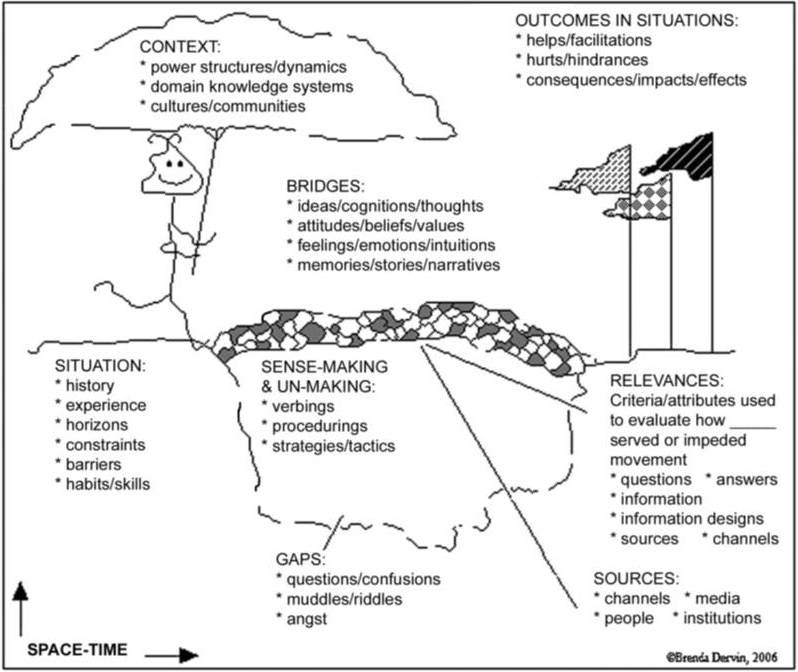
\includegraphics[width=\columnwidth]{dervin}
	\caption{The gap-bridging metaphor of sensemaking. People encounter gaps when moving through time-space, then seek for information, evaluate and use it to bridge the gaps. \is{Dervin2012}}
	\label{fig:lr-dervin}
\end{figure}

Dervin also implements the theory into a set of questions that can be used in interview to understand sensemaking within a context~\cite{Dervin1983}. The questions elaborate all parts of the model, aiming to establish an understanding on the situation (\emph{What happened?}), the gap (\emph{What did you struggle with?}), the bridge (\emph{What idea did you come to?}) and the outcome (\emph{How did that help?}).

\subsection{Learning Loop Complex}
In the context of human-computer interaction, Russell~et~al.~\cite{Russell1993} defines sensemaking as the process of searching for a representation and encoding data in that representation to answer task-specific questions. That cyclic process is called the \emph{learning loop complex} as illustrated in \autoref{fig:lr-russell}. First, the sensemaker searches for a representation to capture salient features of the data (\emph{Generation Loop}). During sensemaking, new information is sought and encoded into this representation (\emph{Data Coverage Loop}). The data unfit to the representation (\emph{residue}) requires the sensemaker to adjusts and produces a more suitable one. This entire learning loop complex is guided by the task with an aim to reduce its cost.

\begin{figure}[!htb]
	\centering
	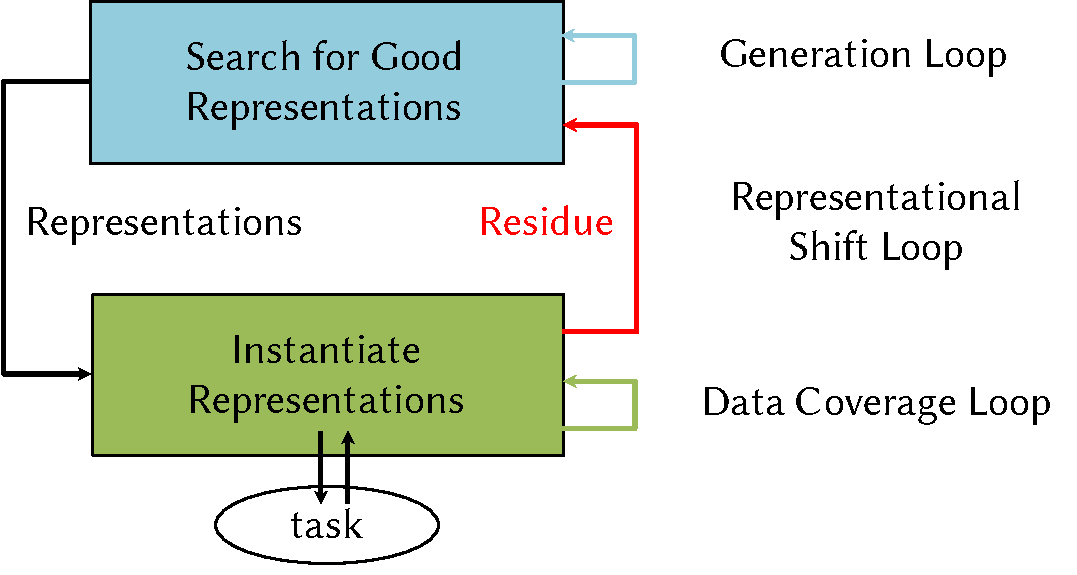
\includegraphics{russell}
	\caption{The learning loop complex theory of sensemaking. It consists of three iterative loops: searching for a good representation, encoding data to the representation, and adjusting the representation for a better data coverage. \is{Russell1993}}
	\label{fig:lr-russell}
\end{figure}

\subsection{Sensemaking in Organizations}
Different from Dervin and Russell who study sensemaking for individuals, Weick focuses on sensemaking at an organization level~\cite{Weick1995}. He proposes that sensemaking consists of these seven following properties.

\begin{enumerate}
	\item \emph{Grounded in identity construction}. Who people think they are, both individually and collectively, affect what they interpret and act.
	\item \emph{Retrospective}. People look back and make sense from what they have said and what they have done before.
	\item \emph{Enactive of sensible environments}. People make sense and contribute to the environments during their sensemaking processes.
	\item \emph{Social}. This is an inherent property of sensemaking in organization where people interact and socialize with others, and also are influenced by others.
	\item \emph{Ongoing}. Sensemaking is a continuous flow because the world and our understanding about the word are constantly changing.
	\item \emph{Focused on and by extracted cues}. Cues are things from the context that people have attention to and may use them to guide further exploration and assessment of the sensemaking problem.
	\item \emph{Driven by plausibility rather than accuracy}. Sensemaking is about plausibility and sufficiency rather than accuracy and completeness. People tend to stop searching when they find an acceptable solution.
\end{enumerate}

\subsection{A Process Model}
\label{sub:lr-pcm}
Pirolli and Card~\cite{Pirolli2005} describe sensemaking as an iterative process that gradually transforms raw data into rational knowledge. The process includes two sets of activities: one that cycles around finding relevant information, and another that cycles around making sense of that information, with plenty of interaction between them. They map to the \emph{foraging loop} and the \emph{sensemaking loop} respectively, as shown in \autoref{fig:lr-pirolli-card-model}. The sensemaking process can progress upward (from data to knowledge) or downward (from knowledge to data). The steps in the \emph{bottom-up} process are summarized as follows.

\begin{figure}[!htb]
	\centering
	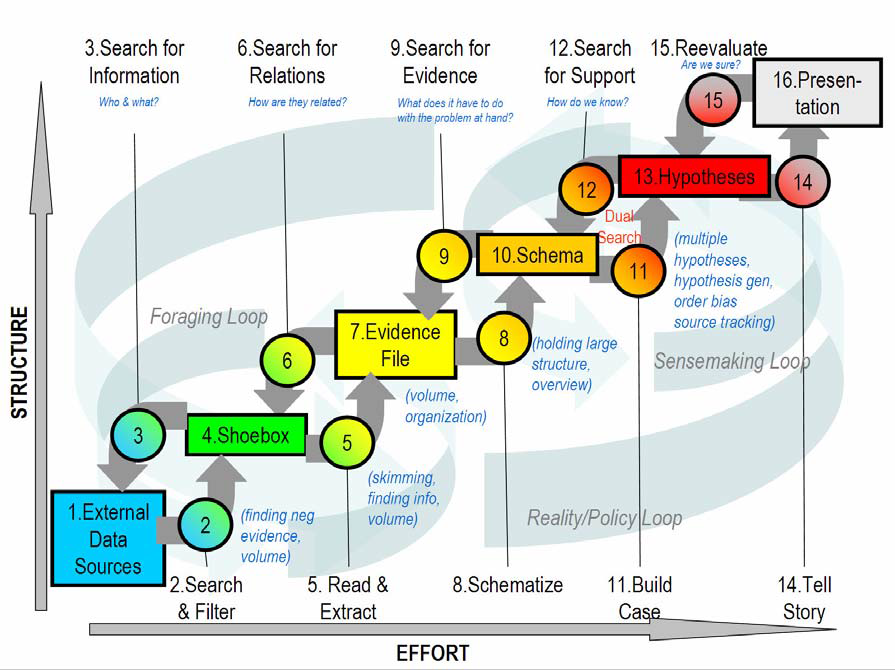
\includegraphics[width=\columnwidth]{pirolli-card-model}
	\caption{A notional model of sensemaking. The sub-processes (numbered circles) and their data input/output (numbered rectangles) are arranged in a two-dimensional space, in which the horizontal axis represents the degree of effort from users, and the vertical axis represents the degree of structure in information representation. \is{Pirolli2005}}
	\label{fig:lr-pirolli-card-model}
\end{figure}

\begin{itemize}
	\item \emph{Search and filter}. External data sources, such as classified databases or the web, are searched and filtered to retrieve relevant documents to the task.
	\item \emph{Read and extract}. These documents are examined to extract pieces of information that may be used as evidence later.
	\item \emph{Schematize}.  The collected information is organized in a way that aids the analysis. This may be executed in user mind, using paper and pen, or with a complex computer-based system.
	\item \emph{Build case}. Multiple hypotheses are generated; evidence are marshaled to support or disconfirm them.
	\item \emph{Tell story}. Discovered cases are presented to some audience.
\end{itemize}

In this model, \emph{schematization} plays an important role in converting raw evidence to rational explanations, bridging the foraging and sensemaking loops. A study by Kang, Görg and John Stasko~\cite{Kang2011} agrees with this observation. In their study, all the participants who performed the sensemaking task well spent considerable time and effort in organizing their collected information. Their organizational schemes were flexible: a \emph{timeline} of related events, a \emph{map} connecting locations that a person has been to, and a \emph{diagram} showing relationships among suspicious targets.

\subsection{Data--Frame Model}
\label{sub:lr-dfm}
Klein et al.~\cite{Klein2003} propose a sensemaking model that centers around \emph{data} and \emph{frame}. Data is the information that a person receives or searches for, and frame is the mental structure that organizes and explains the relationship of such data. For instance, a frame can be a \emph{story}, explaining the chronology of events and the causal relationships between
them; or a \emph{map}, showing where the events take place and the routes between them. Sensemaking is considered as a deliberate effort to understand an event, starting when a person realizes a gap of their current understanding of that event. Klein and his associates describe seven activities involved in sensemaking and are summarized in \autoref{fig:lr-data-frame-model}.

\begin{figure}[!htb]
	\centering
	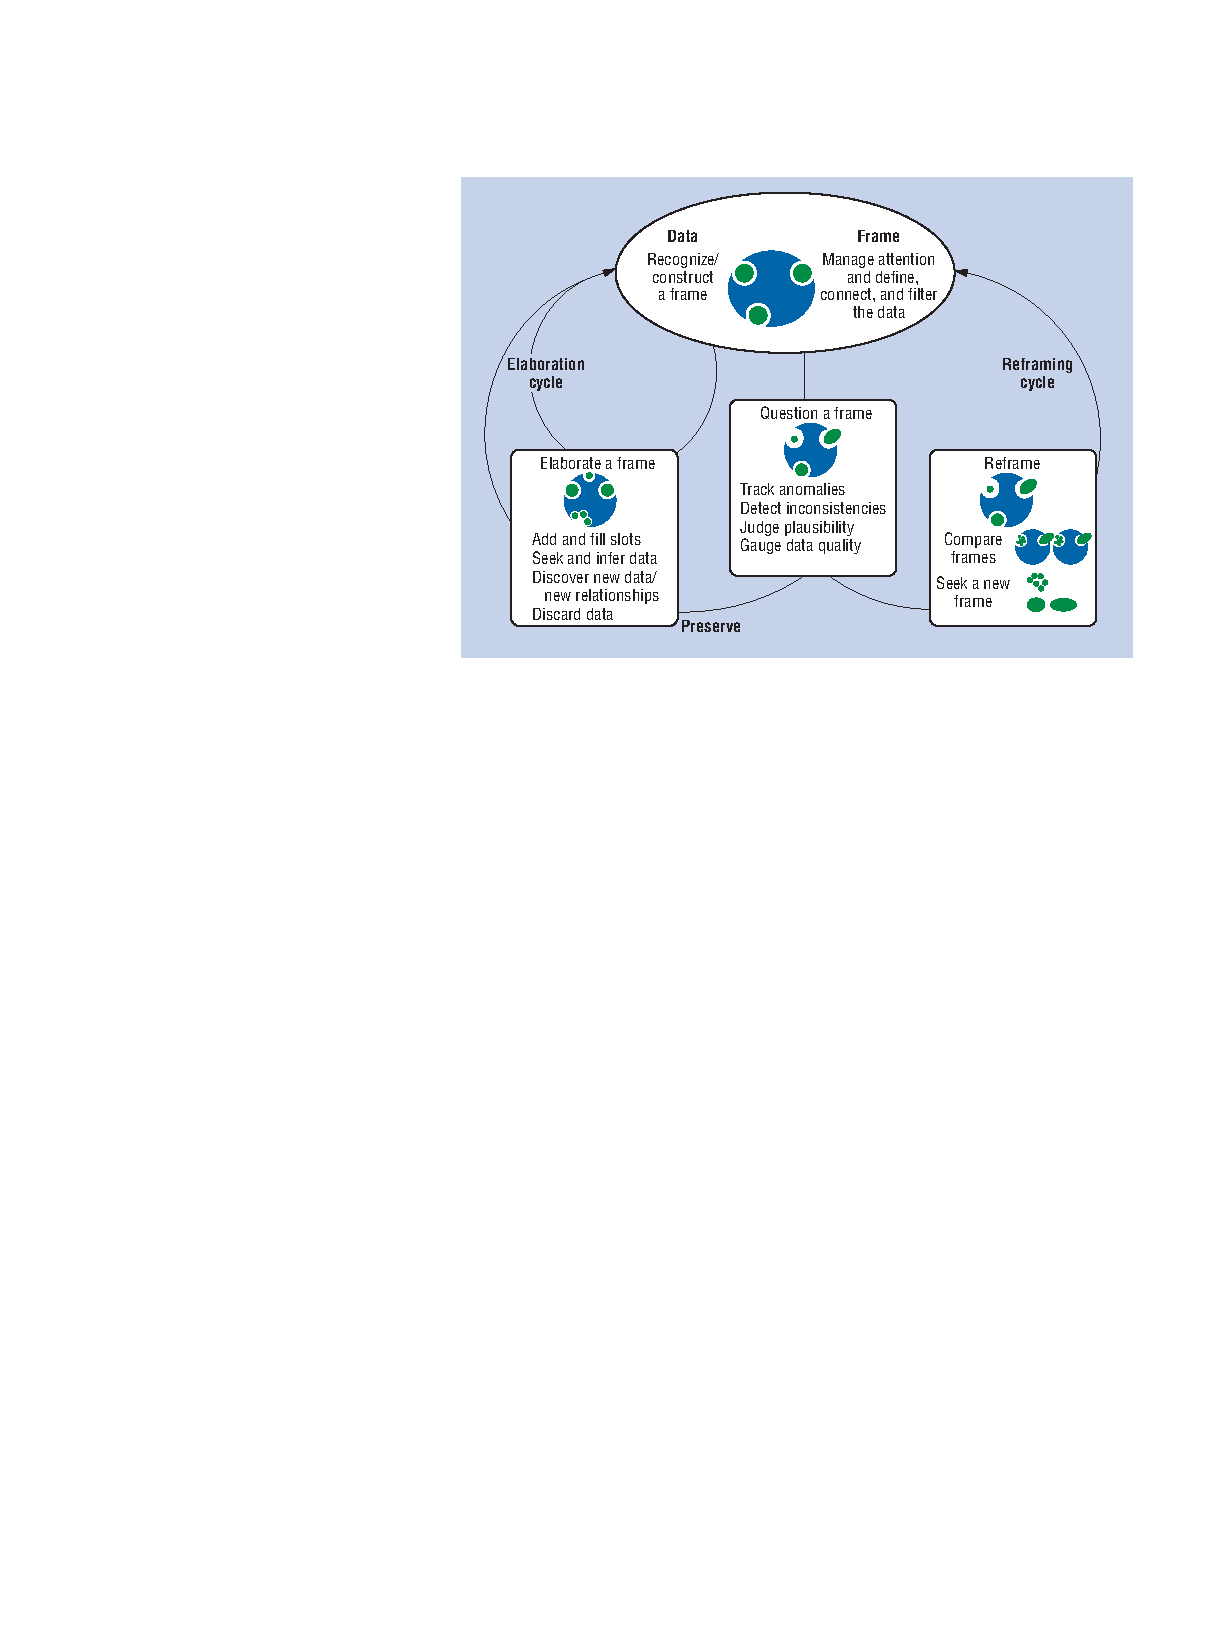
\includegraphics[width=\columnwidth]{data-frame-model}
	\caption{The data--frame model of sensemaking. It describes a set of interconnected sensemaking activities centering around data and frame -- the explanatory structure of data. \is{Klein2003}}
	\label{fig:lr-data-frame-model}
\end{figure}

\begin{itemize}
	\item \emph{Connect data and a frame}. A person recognizes relevant pieces of data and constructs an initial frame to explain them. The frame then helps the person to filter and search for new data.
	\item \emph{Elaborate the frame}. As more is learned about the situation, the frame becomes more elaborate with new data and new relationships. 
	\item \emph{Question the frame}. It happens when a person encounters data that is inconsistent with the existing frame. At this point, the person may be unsure that the frame is incorrect, or the inconsistent data is inaccurate.
	\item \emph{Preserve the frame}. A person may consider the severity of the inconsistent data, justify why it mismatches the frame, and ignore it.
	\item \emph{Compare multiple frames}. Depending on experience, a person may think of alternative frames explaining the same set of data. These frames need to be compared to select the most likely one.
	\item \emph{Reframe}. When encountering inconsistent and contrary data, the person may need to find a replacement that can explain all data. Considering discarded data and/or reinterpreting data could facilitate this activity.
	\item \emph{Seek a new frame}. A person may deliberately search for a new frame when encountering plenty of conflicted data. One or two key data elements may serve as \emph{anchors} to help the person to elicit another frame.
\end{itemize}

The Pirolli and Card's model describes a step-by-step process of sensemaking, in which the analyst collects relevant data and eventually transposes it into rational answers. However, the various sensemaking activities in the Data--Frame model may explain the strategies used by the analyst more comprehensively.

TODO: summary
A recent and comprehensive review of sensemaking can be found in the article by Maitlis and Christianson~\cite{Maitlis2014}.
%\section{Visualization and Visual Analytics}

\subsection{Overview}
Computer-based visualization systems provide visual representations of datasets designed to help people carry out tasks more effectively~\cite{Munzner2014}. Because the design space of possible visual ``idioms'' is huge, it is challenging to create effective visualizations. Understanding well-established information design principles and interaction techniques could guide designers toward the right direction. Also, every visualization needs to be evaluated to check whether it meets its design purposes and how it helps or hinder users.

Overview: what is vis? what can vis help? what is VA? what can VA help, in addition to vis? explain the VA process model. briefly explain the 3 important blocks in the model, which are then discussed in detail next. 

%What is vis? Classic example. What vis can help from cognition (Ben) and Wijk, Fekete?
%
%Large datasets -> simple aggregation, reduction like filtering, interaction, ; larger datasets, more sophiscated emthods extract patterns and vis to display them. and allow further. That is the idea of visual analytics. Orginal def, new def. Model.
%
%Describe visual analytics process model (Figure~\ref{fig:visual-analytics-process})
%
%\begin{figure}[!htb]
%	\centering
%	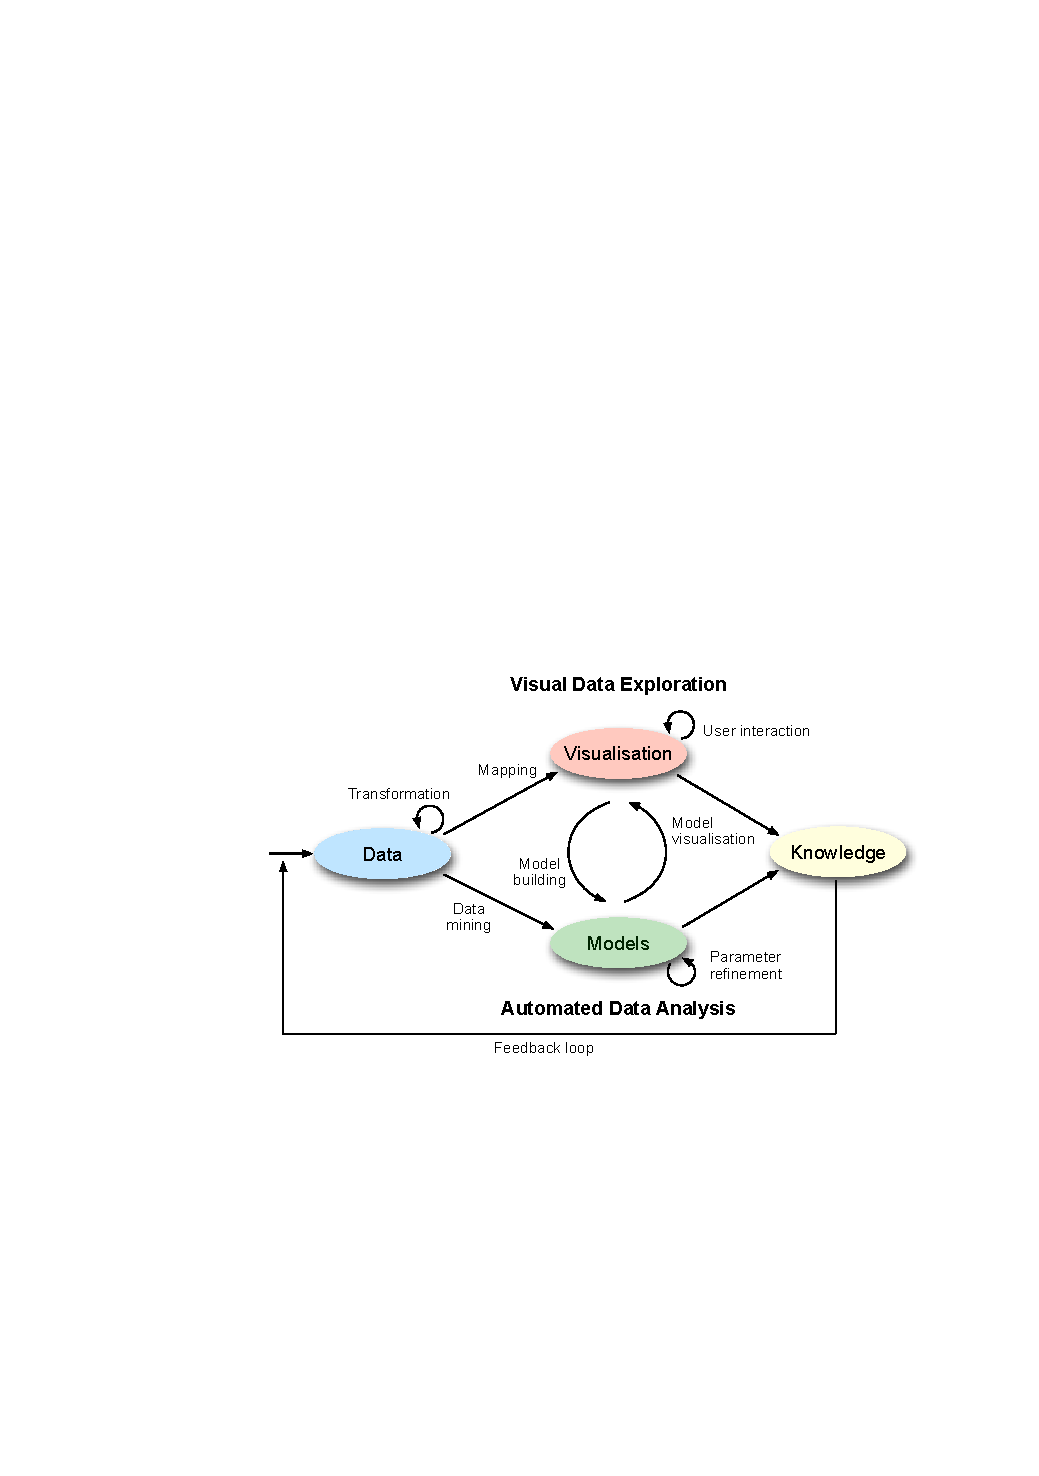
\includegraphics[width=\columnwidth]{visual-analytics-process}
%	\caption{The visual analytics process model. \emph{Source:~\cite{Keim2010}}.}
%	\label{fig:visual-analytics-process}
%\end{figure}
%
%
%Next, discuss basics of vis and models. and evaluation.

\subsection{Visualization Design}


\subsubsection{Information Design Principles}
\label{sub:lr-design}

\paragraph{Marks and Channels}
Marks are basic geometric elements that depict items or links, and channels control their appearance~\cite{Munzner2014}. Item marks can be zero-dimensional as a \emph{point}, one-dimensional as a \emph{line}, two-dimensional as an \emph{area}, and three-dimensional as a \emph{volume}, but rarely used. Link marks include \emph{connection} showing a pairwise relationship between two items using a line and \emph{containment} showing hierarchical relationships using areas. \autoref{fig:lr-marks} illustrates these marks. 

\begin{figure}[!htb]
	\centering
	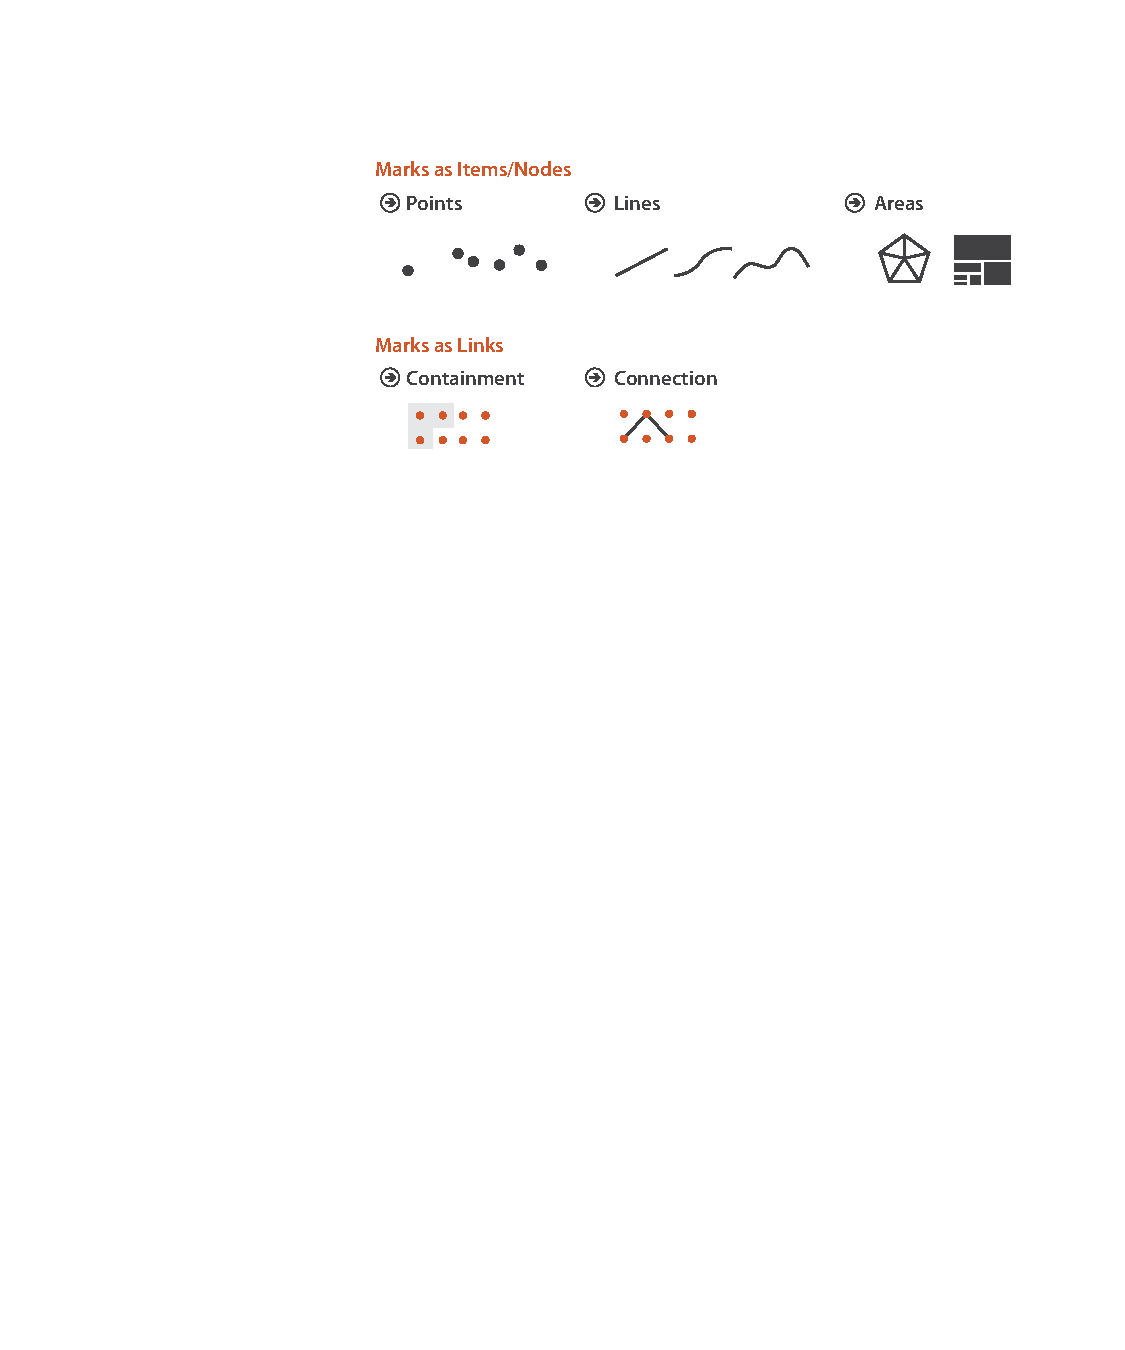
\includegraphics[width=.8\linewidth]{marks}
	\caption{Item and link marks as geometric primitives. \is{Munzner2014}}
	\label{fig:lr-marks}
\end{figure}

A visual channel control the appearance of marks, independent of their dimensionality. Examples include position, color, shape, angle and size. However, not all channels can be applied to all marks. For instance, an area mark is used in a geographic map to denote a region. It is already associated with a shape and size, thus cannot be size coded to represent another quantitative attribute.
some visual channels. some cannot encode size, example. \autoref{fig:lr-channel-example} shows a progression of chart types, with each showing one more data attribute using one more visual channel. \autoref{fig:lr-channel-example-1} shows a bar chart representing a single quantitative attribute using the \emph{vertical position} channel. \autoref{fig:lr-channel-example-2} shows a scatter plot encoding the second quantitative attribute using the \emph{horizontal position} channel. \autoref{fig:lr-channel-example-3} adds the \emph{color} channel to represent a categorical attribute, and \autoref{fig:lr-channel-example-4} adds the \emph{size} channel to represent another quantitative attribute. In these examples, each attribute is encoded with a single channel. However, multiple channels can be combined to redundantly encode the same attribute, helping perceive it more easily.

\begin{figure}[!htb]
\centering
\subcaptionbox{Line marks with horizontal position for a categorical attribute and vertical position for a quantitative attribute.\label{fig:lr-channel-example-1}}{
\includegraphics[width=.23\columnwidth]{channel-example-1}} 
\hfill
\subcaptionbox{Point marks with both horizontal and vertical position channels for quantitative attributes.\label{fig:lr-channel-example-2}}{
\includegraphics[width=.23\columnwidth]{channel-example-2}} 
\hfill
\subcaptionbox{A categorical attribute is added using the color channel.\label{fig:lr-channel-example-3}}{
\includegraphics[width=.23\columnwidth]{channel-example-3}}
\hfill
\subcaptionbox{Another quantitative attribute is added using the size channel.\label{fig:lr-channel-example-4}}{
\includegraphics[width=.23\columnwidth]{channel-example-4}}
\caption{Using marks and channels.}
\label{fig:lr-channel-example}
\end{figure}

All channels are not equal; they are processed and perceived differently by our human visual systems. Also, not all channels are appropriate for encoding both ordered and categorical attributes. Ordered attributes should be shown using magnitude channels, with \emph{aligned spatial position} as the most effective channel and \emph{3D volume} as the least effective one. Categorical attributes should be shown using identity channels, with \emph{spatial region} as the most effective channel and \emph{shape} as the least effective one. \autoref{fig:lr-channel-ranking} shows the detailed ranking of effectiveness of many visual channels, separated by the type of attribute. This ranking is documented by Munzner~\cite{Munzner2014}, based on many empirical studies such as the work by Cleveland and McGill~\cite{Cleveland1985}, and by Heer and Bostock~\cite{Heer2010a}.

\begin{figure}[!htb]
	\centering
	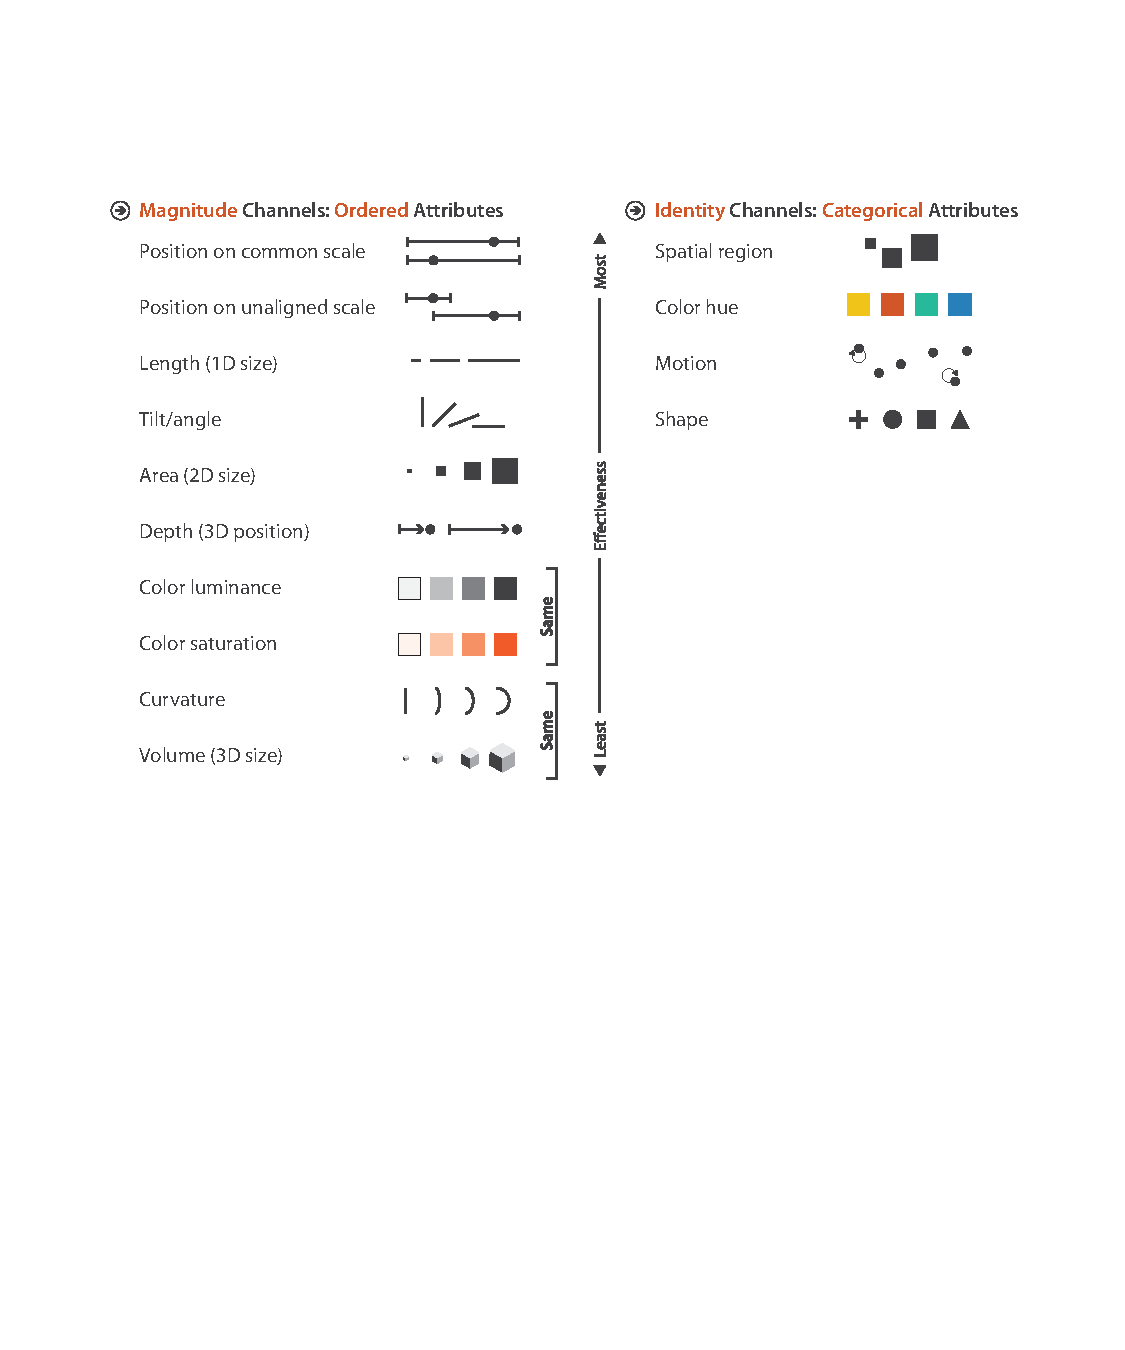
\includegraphics[width=\linewidth]{channel-ranking}
	\caption{Channels ranked by effectiveness according to data and channel type. \is{Munzner2014}}
	\label{fig:lr-channel-ranking}
\end{figure}

Color is a special channel that can be used for both data attributes. As shown in \autoref{fig:lr-channel-ranking}, color luminance and saturation are used in magnitude channels, and color hue is used in identity channels. A colormap specifies a mapping between colors and data values, and designing an effective colormap is challenging. ColorBrewer~\cite{Harrower2003} is an excellent source for colormap reference, providing color schemes for both categorical and ordered attributes. Human can only distinguish around 12 colors simultaneously~\cite{Munzner2014}. \autoref{fig:lr-colorbrewer-1} shows such a categorical colormap with 12 distinguished color hues. Ordered colormaps can be either sequential (\autoref{fig:lr-colorbrewer-2}) or diverging (\autoref{fig:lr-colorbrewer-3}). Diverging colormaps use two different color hues to emphasize values below and above the middle point.

\begin{figure}[!htb]
\centering
\subcaptionbox{Categorical colormap with distinguishable color hues.\label{fig:lr-colorbrewer-1}}[\columnwidth]{
\includegraphics[width=.6\columnwidth]{colorbrewer-1}} 
\\
\subcaptionbox{Sequential colormap: a single color hue with different saturation level.\label{fig:lr-colorbrewer-2}}[\columnwidth]{\hspace{-.15\columnwidth}
\includegraphics[width=.45\columnwidth]{colorbrewer-2}}
\\
\subcaptionbox{Diverging colormap: two color hues emphasizing positive and negative values.\label{fig:lr-colorbrewer-3}}[\columnwidth]{\hspace{-.05\columnwidth} 
\includegraphics[width=.55\columnwidth]{colorbrewer-3}}
\caption{Colormaps from ColorBrewer. \is{Harrower2003}}
\end{figure}

\subparagraph{Gestalt Principles}
\label{sub:lr-gestalt}
Gestalt principles describe how we see patterns in visual displays~\cite{Koffka1935}. This section reviews three commonly used principles in representing groups of items.

\subparagraph{Similarity} 
Similar elements tend to be grouped together. \autoref{fig:lr-gestalt-similarity-1} shows a matrix of point marks with uniform spacing, but using two different shapes: dot and cross. The similarity of shapes helps us see the rows more clearly than the columns. Two separable channels can be applied together to reveal patterns by either rows or columns. In \autoref{fig:lr-gestalt-similarity-2}, green is used to depict rows, and texture is used to depict columns.

\begin{figure}[!htb]
\centering
\subcaptionbox{Similarity of shapes distinguishes rows.\label{fig:lr-gestalt-similarity-1}}[.47\columnwidth]{
\includegraphics[height=.35\columnwidth]{gestalt-similarity-1}} 
\hfill
\subcaptionbox{Color and texture delineate rows and columns, respectively.\label{fig:lr-gestalt-similarity-2}}[.47\columnwidth]{
\includegraphics[height=.35\columnwidth]{gestalt-similarity-2}} \label{fig:lr-gestalt-similarity}
\caption{Similarity principle: similar elements are perceived as a group. \is{Ware2013}}
\end{figure}

\subparagraph{Proximity} 
Elements that are close together are perceptually grouped together. \autoref{fig:lr-gestalt-proximity-1} clearly shows two groups of dots. \autoref{fig:lr-gestalt-proximity-2} shows rows of dots. However, with a small change of spacing, these dots are perceived as columns in \autoref{fig:lr-gestalt-proximity-3}. The application of this principle is straightforward: organizing related information close together. It helps separate groups of unrelated objects and facilitates searching for information.

\begin{figure}[!htb]
\centering
\subcaptionbox{Two groups of dots.\label{fig:lr-gestalt-proximity-1}}{
\includegraphics[width=.25\columnwidth]{gestalt-proximity-1}} 
\hfill
\subcaptionbox{Rows of dots.\label{fig:lr-gestalt-proximity-2}}{
\includegraphics[width=.31\columnwidth]{gestalt-proximity-2}} 
\hfill
\subcaptionbox{Columns of dots.\label{fig:lr-gestalt-proximity-3}}{
\includegraphics[width=.31\columnwidth]{gestalt-proximity-3}}
\label{fig:lr-gestalt-proximity}
\caption{Spatial proximity principle: spatially close elements are perceived as a group. \is{Ware2013}}
\end{figure}

\paragraph{Connectedness} 
Elements that are connected by visual properties are perceived as being more related than elements that are not connected. This principle can be achieved simply by drawing a border around a group of elements as in \autoref{fig:lr-gestalt-connectedness-1}. This is extensively applied in designing complex graphical user interface: groups of related features are separated by borders. Another approach to implement connectedness is by drawing lines between related elements as in \autoref{fig:lr-gestalt-connectedness-2}. This is the basics of \emph{node-link diagrams} -- one of the most common methods of representing relationships between elements.

\begin{figure}[!htb]
\centering
\subcaptionbox{Using border to denote a group.\label{fig:lr-gestalt-connectedness-1}}{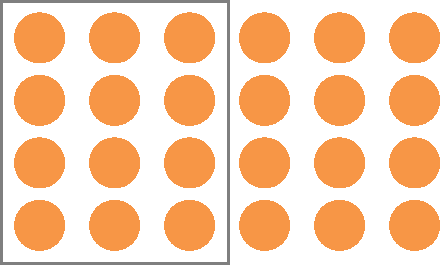
\includegraphics[width=.4\columnwidth]{gestalt-connectedness-1}} 
\hfill
\subcaptionbox{Using lines to denote a group.\label{fig:lr-gestalt-connectedness-2}}{
\includegraphics[width=.4\columnwidth]{gestalt-connectedness-2}} 
\caption{Connectedness principle: visually connected elements are perceived as a group. \is{Ware2013}}
\label{fig:lr-gestalt-connectedness}
\end{figure}

Among these three Gestalt principles of representing groups of elements, connectedness has the strongest effect, followed by proximity and then similarity. \autoref{fig:lr-gestalt} illustrates this comparison. In \autoref{fig:lr-gestalt-1}, even though spacing between dots in rows is shorter than spacing between dots in columns, the lines make the vertical links clearer than rows. In \autoref{fig:lr-gestalt-2}, the lines also make the horizontal links more notable than groups of colored circles. In \autoref{fig:lr-gestalt-3}, two spatial groups are more clearly perceived than colored groups.

\begin{figure}[!htb]
\centering
\subcaptionbox{Links are more clearly perceived than spatial groups.\label{fig:lr-gestalt-1}}[.3\columnwidth]{
\includegraphics[height=.12\columnwidth]{gestalt-1}} 
\hfill
\subcaptionbox{Links are more clearly perceived than colored groups.\label{fig:lr-gestalt-2}}[.3\columnwidth]{
\includegraphics[height=.12\columnwidth]{gestalt-2}} 
\hfill
\subcaptionbox{Spatial groups are more clearly perceived than colored groups.\label{fig:lr-gestalt-3}}[.3\columnwidth]{
\includegraphics[height=.12\columnwidth]{gestalt-3}}
\caption{Comparison of Gestalt principles. Connectedness is stronger than proximity, and proximity is stronger than similarity. \is{Ware2013}}
\label{fig:lr-gestalt}
\end{figure}

\paragraph{Tufte's Principles}
Tufte proposes a number of principles for a well-designed graphic, documented in his series of books, most notably including \emph{The Visual Display of Quantitative Information}~\cite{Tufte1983} and \emph{Envisioning Information}~\cite{Tufte1990}. This section reviews a few principles that have been commonly applied in graphic design and visualization.

\subparagraph{Graphical Integrity}
This principle emphasizes that the graphical representation should tell the truth about the data. Representation of numbers, as physically measured on the surface of the	graphic	itself,	must be directly proportional to the numerical quantities represented~\cite{Tufte1983}. \autoref{fig:lr-tufte-integrity-1} shows a falsely big drop in stock market value between 2001 and 2002. It because the chart uses a relative scale with the value range from 450 to 500, causing its height disproportional to the market value. \autoref{fig:lr-tufte-integrity-2} corrects this error by using an absolute scale with the value range starting from 0.

\begin{figure}[!htb]
\centering
\subcaptionbox{Using a relative value range causes a falsely big drop of stock market value between 2001 and 2002.\label{fig:lr-tufte-integrity-1}}{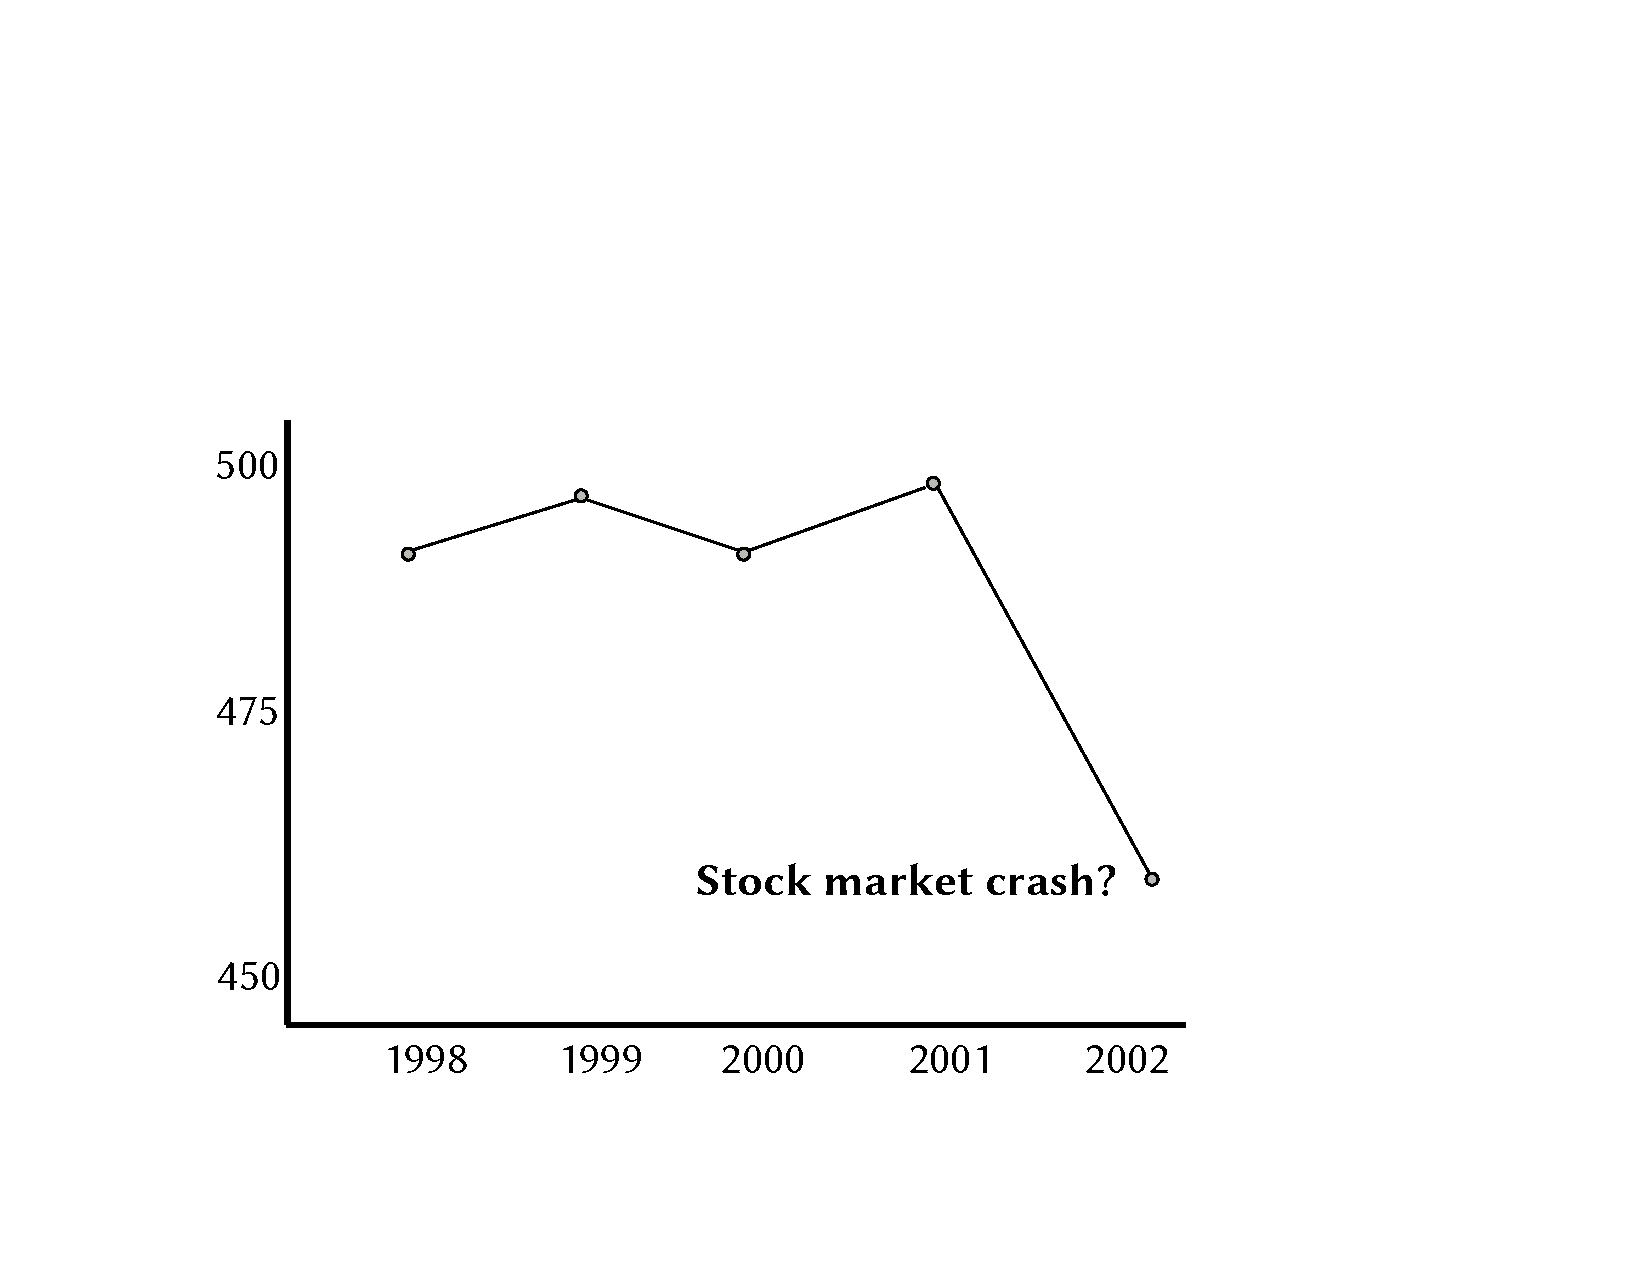
\includegraphics[width=.47\columnwidth]{tufte-integrity-1}} 
\hfill
\subcaptionbox{Using an absolute value range to depict the data accurately.\label{fig:lr-tufte-integrity-2}}{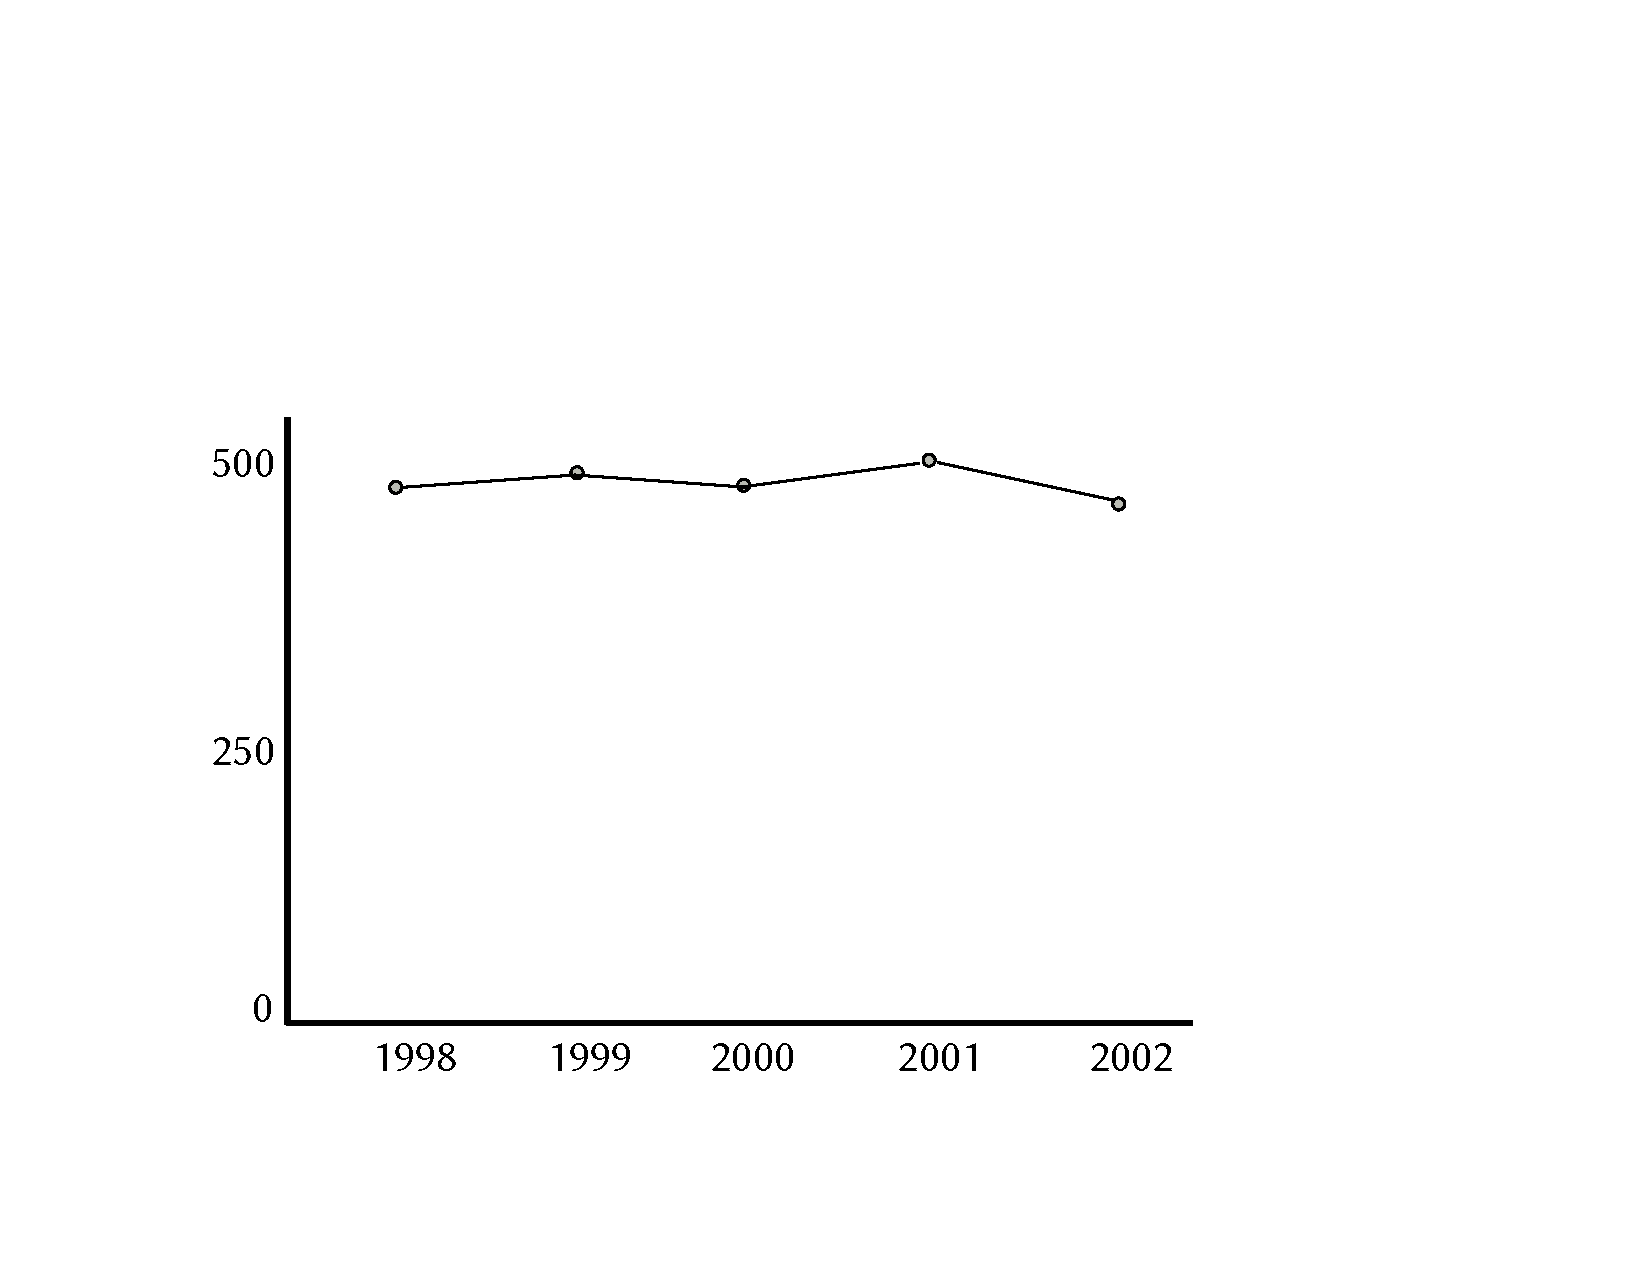
\includegraphics[width=.47\columnwidth]{tufte-integrity-2}} 
\caption{Graphical integrity principle. The chart should tell the truth about the data.}
\label{fig:lr-tufte-integrity}
\end{figure}

\subparagraph{Data-Ink Ratio Maximization}
Data-ink includes the pixels in the graphic that are used for representing the data. Data-ink ratio is defined as the ratio between the data-ink and the total non-background pixels used in the graphic. This principle aims to maximize this ratio by erasing non-data-ink and erasing redundant data-ink.

\begin{figure}[!htb]
\centering
\subcaptionbox{A bar chart with poor data-ink ratio.\label{fig:lr-tufte-ink-1}}{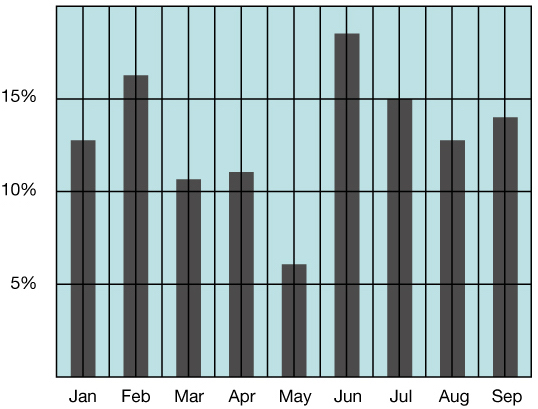
\includegraphics[width=.47\columnwidth]{tufte-ink-1}} 
\hfill
\subcaptionbox{A bar chart with high data-ink ratio by removing background, border and grid lines.\label{fig:lr-tufte-ink-2}}{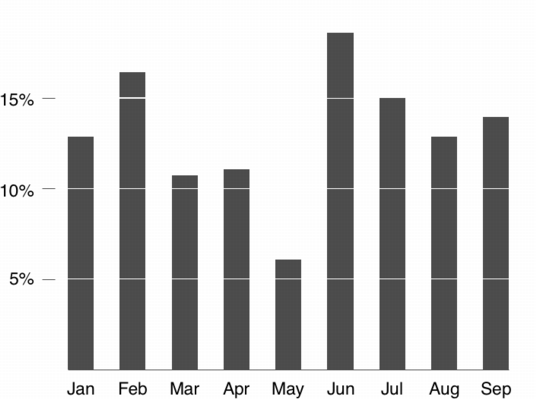
\includegraphics[width=.47\columnwidth]{tufte-ink-2}} 
\caption{Data-ink ratio maximization principle: removing the graphic that does not contribute to the understanding of the data.}
\label{fig:lr-tufte-ink}
\end{figure}
% Source: http://www.infovis-wiki.net/index.php/Data-Ink_Ratio

\subparagraph{Micro/Macro Readings}
This principle suggests that a graphic can contain both enormous details and an overall pattern. This allows the viewer to glance from a distance to observe the big picture, and later drill-down closely to examine its individual pieces. Classic stem-and-leaf plot is a great example to illustrate this principle (\autoref{fig:lr-tufte-micro}). The plot shows all individual data items at meaningful level of detail, and provides an understanding of the data distribution. The micro/macro principle is extensively applied in interactive visualization, where zooming are panning are made possible, such as Google Maps. Data items at different scales can be represented with different levels of detail to provide appropriate information based on the allowed display area.

\begin{figure}[!htb]
	\centering
	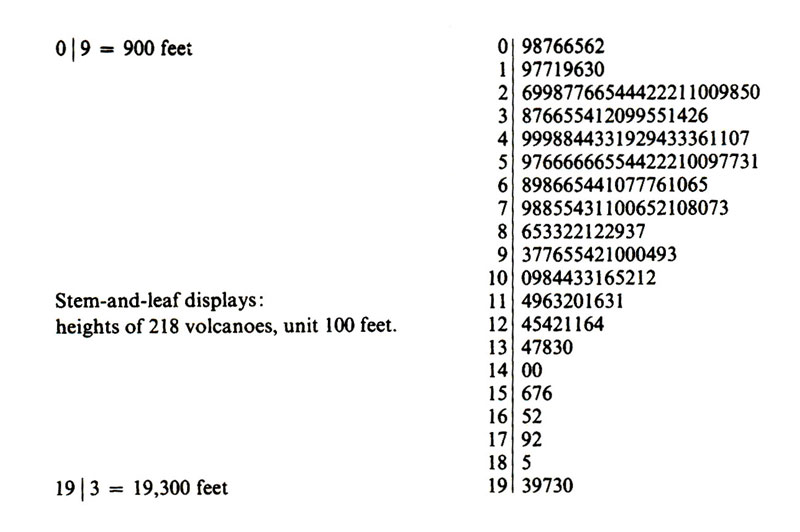
\includegraphics[width=.9\linewidth]{tufte-micro}
	\caption{Micro/macro principle. A stem-and-leaf plot shows both the data distribution and individual items. \is{Tufte1983}}
	\label{fig:lr-tufte-micro}
\end{figure}


%In a broader context, GUI design principles:  Schneiderman~\cite{Shneiderman2016} (eight golden rules), Norman (six design principles) ~\cite{Norman2002} and	Nielsen (ten usability heuristics)~\cite{Nielsen1994} -- create a table with rows showing similar principles
%http://www.csun.edu/science/courses/671/bibliography/preece.html
%https://faculty.washington.edu/jtenenbg/courses/360/f04/sessions/schneidermanGoldenRules.html
%https://www.interaction-design.org/literature/article/shneiderman-s-eight-golden-rules-will-help-you-design-better-interfaces

\subsubsection{Interaction Techniques}
Interaction typically refers to the set of controls provided to the user to manipulate an interface~\cite{Pike2009a}. A static visualization may only show one aspect of a dataset. When the dataset is large enough, showing all the data at once may also make the visualization become cluttered. Interaction plays an important role in solving these problems. It can help explore large datasets at multiple levels of detail, identify patterns through examination of different visual representations and understand the connections between them.

Examples of interaction include standard techniques used in graphical user interface such as mouse clicking and scrolling, and more visualization specific techniques such as \emph{linking and brushing}~\cite{Kosara2003}, and \emph{focus+context}~\cite{Cockburn2008}. Multiple views in a visualization are often linked together to exploit their strengths. The user can select points of interest using the brushing technique, typically done directly on the visual data representation such as dragging a rectangular area. The points are brushed in one view will be highlighted in other views, allowing the user to explore them with different perspectives and representations (\autoref{fig:lr-linking}). Focus+Context is a technique that brings both the overview (context) and the detailed information (focus) together in one view. A fisheye view~\cite{Furnas1986,Furnas2006} is one example of this technique: the focal region is magnified and displayed within its surrounding context (\autoref{fig:lr-fisheye}).

\begin{figure}[!htb]
\centering
\subcaptionbox{Linking and brushing. Data points brushed in one view are linked and highlighted in other views.\label{fig:lr-linking}}{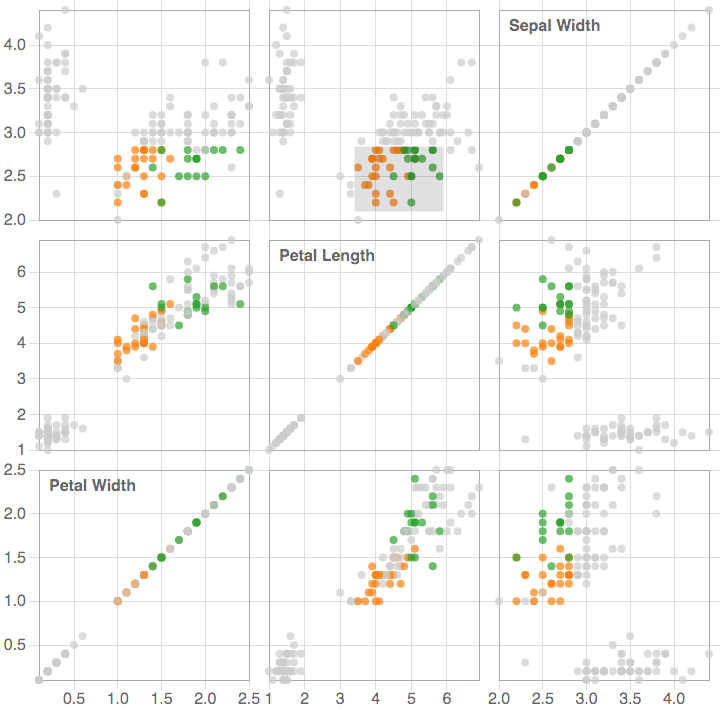
\includegraphics[height=.43\columnwidth]{linking}} 
\hfill
\subcaptionbox{Fisheye view for focus+context. Both the overview and the detailed information are displayed in one view.\label{fig:lr-fisheye}}{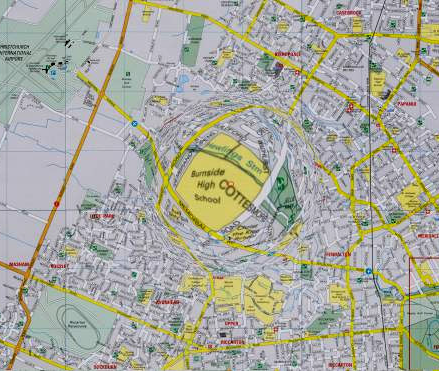
\includegraphics[height=.43\columnwidth]{fisheye}} 
\caption{Examples of interaction techniques.}
\label{fig:lr-interaction}
\end{figure}

Many other interaction techniques can be found in the taxonomies by Dix and Ellis~\cite{Dix1998}, by Keim~\cite{Keim2002}, and by Wilkinson~\cite{Wilkinson2005}. Very often, a user performs an interaction to achieve some goal, thus interaction techniques can also be classified based on their intents. Actually, different interaction techniques in different visualizations may serve the same purpose. For example, both drilling-down a treemap~\cite{Shneiderman1992} and semantic zooming~\cite{Perlin1993} aim to get more details. Taxonomies of high-level interaction can be found in the work by Yi~et~al.~\cite{Yi2007}, by Heer and Shneiderman~\cite{Heer2012}, and by Brehmer and Munzner~\cite{Brehmer2013}. These classifications could help visualization designers select suitable interaction techniques to serve for the capabilities they want to offer to the users.

%Several methods can improve existing different interaction techniques. 
Traditional graphical user interface widgets are often used to control different settings of a visualization, such as buttons and sliders. The disadvantage is that visual feedback does not appear where the interaction happens, but in some parts of the visualization. It also takes time for the user to search for the appropriate setting controllers. Direct manipulation~\cite{Shneiderman1982} is an approach to address these problems. It enables the user to directly interact with the visual representation and receive immediate feedback. One example is using mouse scrolling to adjust zoom level while exploring a map instead of clicking on a button in the toolbar. Another example is parallel coordinates plot with axes can be reordered by direct dragging and values can be filtered by direct brushing on the axes (\autoref{fig:lr-pcp}). Surrogate objects can be used when the data objects are small or distant~\cite{Kwon2011}. An example is the use of interactive legends as filtering means~\cite{Riche2010b}

\begin{figure}[!htb]
	\centering
	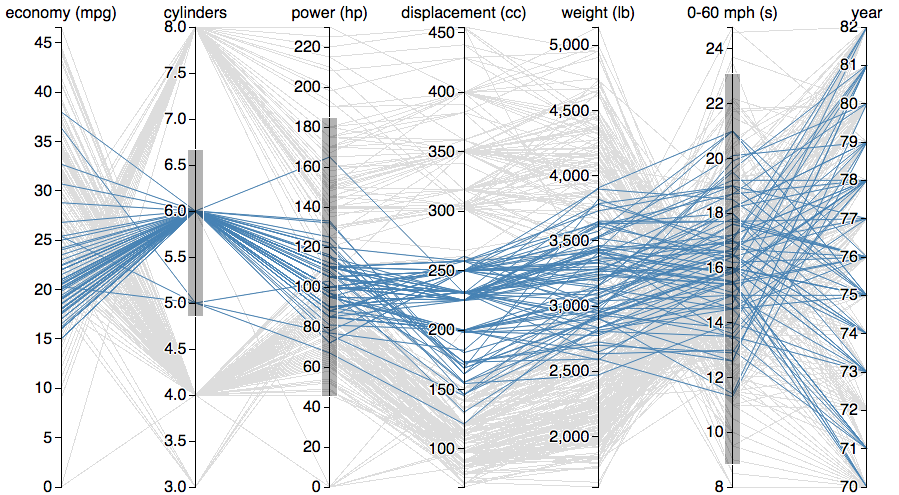
\includegraphics[width=\linewidth]{pcp}
	\caption{Direct manipulation in a parallel coordinates plot with reorder-able and brush-able axes.}
	\label{fig:lr-pcp}
\end{figure}

Another concept that can be applied to improve existing interaction techniques is \emph{fluid interaction}~\cite{Elmqvist2011}. Besides using direct manipulation as discussed previously, the interaction should produce smooth animated transitions between the state before and the state after an interaction, helping users maintain their mental maps; and provide immediate visual feedback, allowing users to know what is happening and/or what will happen next.

Typically, interaction techniques are combined to explore the data or present a known story. A classic visual information-seeking mantra by Shneiderman~\cite{Shneiderman1996} summarizes many design guidelines and interaction techniques for designing information visualizations: \emph{Overview first, zoom and filter, then details-on-demand}. With large datasets, it it challenging to create an overview and provides cues for further exploration. A more suitable approach in this case is \emph{Search, show context, expand on demand}~\cite{VanHam2009}.

\subsection{Automated Analysis Methods}
Data mining is the computational process of extracting patterns in large datasets~\cite{Tan2006}. Data mining tasks can be broadly divided into two major categories:

\begin{itemize}
		\item \emph{Descriptive tasks}. The objective is to derive patterns (correlations, trends, clusters, trajectories and anomalies) that summarizes the underlying relationships in data. Examples include cluster and association analyses. \emph{Clustering} aims to split data items to groups so that items within a group are more similar to each other than those in other groups. For example, clustering can be used to help marketers discover distinct groups of their customers before applying appropriate marketing strategies to those groups. \emph{Association} analysis discovers the connections among a set of data items. For example, it can be used to identify products that customers often purchase together such as bread and milk.
		
		\item \emph{Predictive tasks}. The objective is to predict the value of an unknown (target) attribute based on the values of other (explanatory) attributes. Examples include classification and regression. \emph{Classification} predicts discrete target variables whereas, \emph{regression} focuses on continuous ones. For example, predicting whether a customer buys a marketing product is a classification task because the target variable is binary. However, estimating a future house price is a regression task because price is a continuous-valued variable.
\end{itemize}

Next, we will discuss the clustering and classification tasks in more detail and how they are applied together with visualizations to help users gain deeper insight into the data. We also present some commonly used text mining techniques for exploring large sets of documents, which is essential in visual analytics~\cite{Thomas2005}.

\subsubsection{Clustering}

\paragraph{Overview}
Cluster analysis finds similarities between data points based on the characteristics of data attributes and groups similar data points into clusters. Clustering is regarded as \emph{unsupervised learning}~\cite{Han2011} because it can reveal hidden structure of a dataset that does not have \emph{labels} (or groups) defined. The most common clustering algorithm is \emph{k-means}~\cite{Lloyd1982}. Given a set of data points $(x_1, x_2, \dots, x_n)$, k-means clustering aims to partition them into $k$ clusters $(S_1, S_2, \dots, S_n)$, such that the within-cluster sum of squared distances is minimized: 
\[
\sum_{i=1}^k\sum_{x\in S_i} \lVert x-\mu_i \rVert^2
\]
where $\mu_i$ is the center of points (i.e., centroids) in $S_i$. 

The algorithms works as follows. Initially, partition data points into $k$ non-empty random subsets. Then, compute the centroids of the current clusters, and assign each data point to the cluster with the nearest centroid. Repeatedly recompute the centroids and reassign the cluster of each data point until no assignment can be done. This k-means clustering algorithm is efficient but often terminates at a local optimal. More detailed analysis of k-means and other clustering algorithms are out of the scope of this thesis and can be found in data mining textbooks~\cite{Tan2006,Han2011}.

\paragraph{Application Examples}
Human motion tracking data has been applied in various research fields such as medicine, sports and animation~\cite{Bernard2013}. The data consists of temporal sequences of human poses represented by a set of 3D joint positions (e.g., head, hands, elbows and knees). However, analyzing a large collection of such temporal and high-dimensional datasets is challenging. To gain an overall understanding of the data, MotionFlow~\cite{Jang2016} applies a k-means clustering method using a simple Euclidean distance of 3D joints as the similarity measurement. A cluster of human poses is represented as a glyph with a stick figure showing the centroid of the cluster and semi-transparent ghosts around the center figure for other similar poses (\autoref{fig:lr-MotionFlow}).

\begin{figure}[!htb]
	\centering
	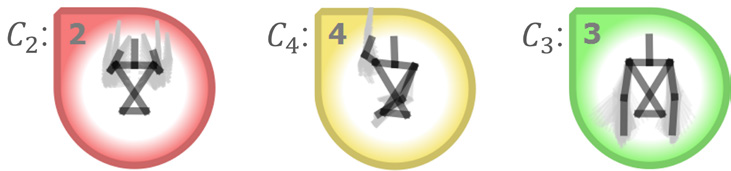
\includegraphics[width=.8\linewidth]{clus-MotionFlow}
	\caption{Visual representation of human pose clusters. \is{Jang2016}}
	\label{fig:lr-MotionFlow}
\end{figure}

MotionFlow uses a force-directed graph of clusters to illustrate their relationship with node distance mapping to the similarity of pose clusters and edges indicating the directed transition between two clusters. Edges are color coded to represent the transition frequency. A user is allowed to interactively change the number of clusters, enabling exploration of the dataset. However, the re-clustering process may change all existing clusters and make it difficult for the user to keep track. To address this issue, MotionFlow allows the user to select the clusters to be locked or unchanged during the re-clustering process. He or she is also able to interactively merge or split clusters according to his or her own assessment.

To achieve the same objective of gaining an overall understanding of human motion tracking data, MotionExplorer~\cite{Bernard2013} applies a different cluster analysis method -- hierarchical clustering~\cite{Han2011} -- which seeks to build a hierarchy of clusters. MotionExplorer takes a divisive approach considering all data items starting within the same cluster and splitting them until a termination condition is met. One of the important decisions in this clustering technique is to determine which cluster to split next. The user is allowed to choose among several splitting strategies such as \emph{maximum standard deviation} to split the most varied cluster first and \emph{highest number of elements} to split the largest cluster first. The hierarchy is visualized as a dendrogram as in \autoref{fig:lr-MotionExplorer}. Clusters are obtained by cutting the dendrogram at the desired vertical level: each connected branch forms a cluster. The vertical axis of the dendrogram can encode different variables depending on the splitting strategy. In \autoref{fig:lr-MotionExplorer}, it shows the standard deviation of each cluster and the user is allowed to slide the cutting value to adjust the resulting clusters.

\begin{figure}[!htb]
	\centering
	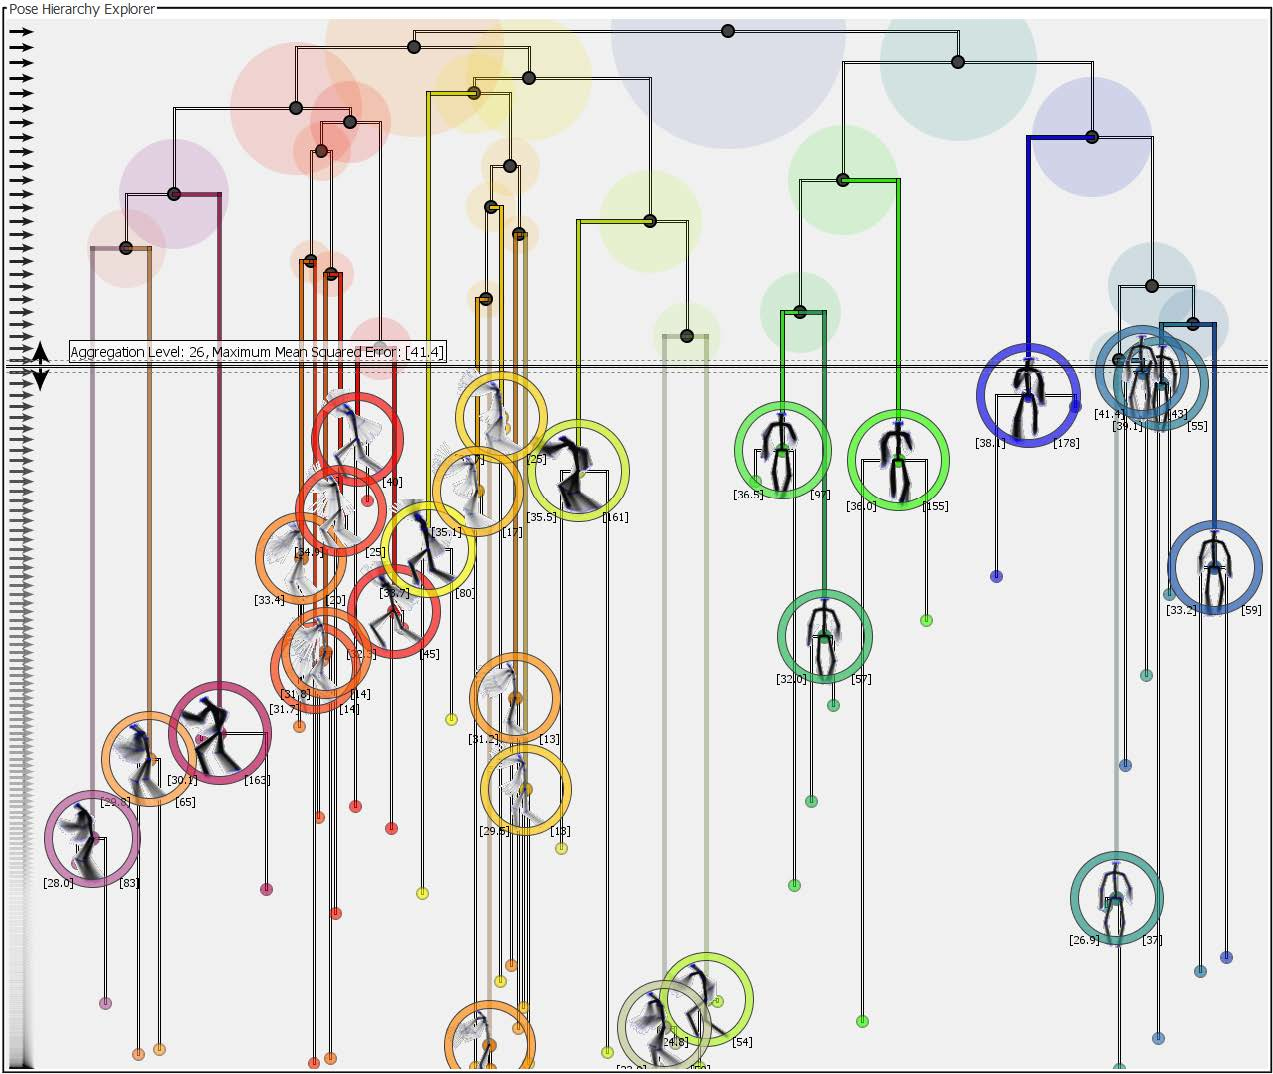
\includegraphics[width=\linewidth]{clus-MotionExplorer}
	\caption{A divisive hierarchical clustering of human poses visualized as a dendrogram. \is{Bernard2013}}
	\label{fig:lr-MotionExplorer}
\end{figure}

A different approach in hierarchical clustering is bottom-up or agglomerative clustering. The process starts with singleton clusters before merging the most similar clusters together until a termination condition is met. NewsLab~\cite{Ghoniem2007} applies such an approach in analysis of large scale broadcast news video collections. It builds a hierarchy of clusters over all keywords extracted from available video captions based on their co-occurrences in the news stories. Therefore, strongly correlated keywords are grouped into the same clusters whereas loosely related keywords are separate in different clusters. Each cluster is visualized as a stream showing the evolution of the keywords within the cluster over time with closely related clusters placed close to each other to allow navigation to different depths of the cluster hierarchy (\autoref{fig:lr-NewsLab}).

\begin{figure}[!htb]
	\centering
	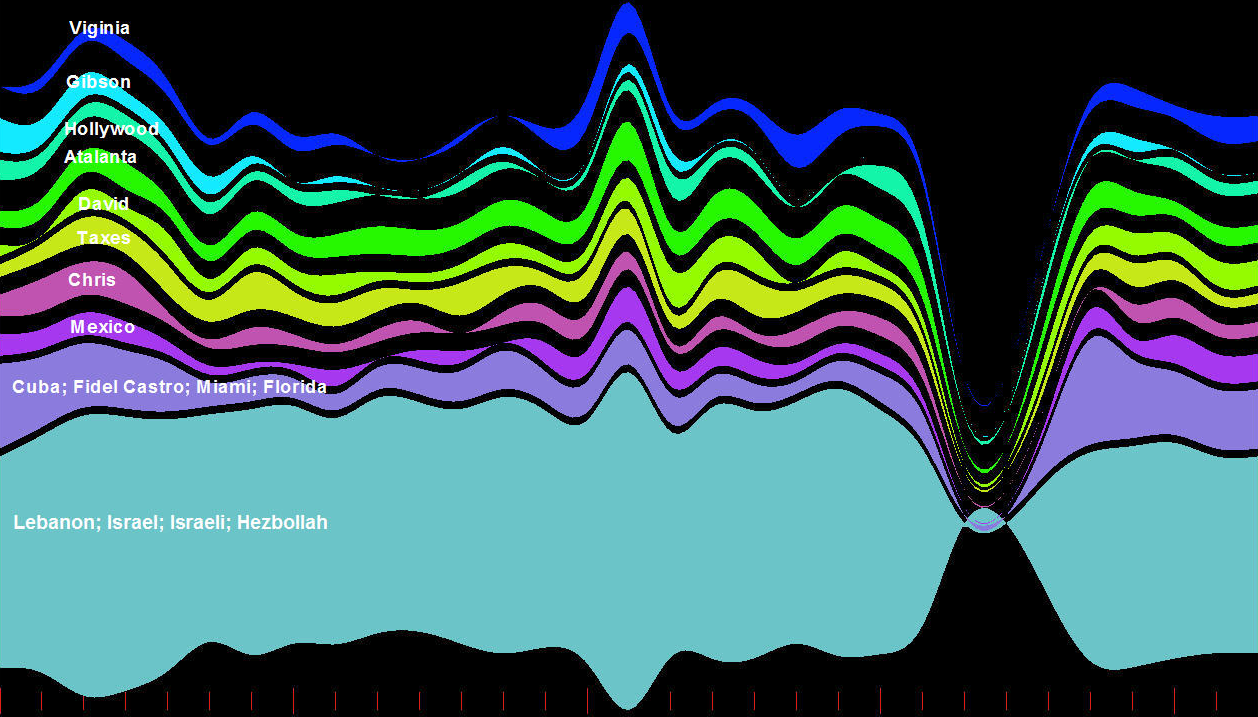
\includegraphics[width=\linewidth]{clus-NewsLab}
	\caption{An agglomerative hierarchical clustering of video captions visualized as streams. \is{Ghoniem2007}}
	\label{fig:lr-NewsLab}
\end{figure}

Understanding people movement patterns in both space and time plays an important role in urban planing. Analyzing and presenting large and complex datasets that contain a number of people in different places and their movement between those places over time are challenging. Mobility Graphs~\cite{Landesberger2016} applies cluster analysis to simplify the data in both spatial and temporal dimensions to gain an overall understanding of the datasets. First, it aggregates places using a density-based clustering technique that considers both the density of places and their flow magnitudes so that close and highly connected can be grouped together. Second, temporal aggregation groups the time steps by the similarity of those simplified places using a k-means clustering technique. \autoref{fig:lr-MobilityGraphs} shows 7 temporal clusters of simplified places. The clusters are color coded with a calendar view to reveal temporal patterns over a week. In each cluster, a node shows an aggregated place with size corresponding to the total number of people in all individual places and arrow widths representing the number of people moving between two aggregated places.

\begin{figure}[!htb]
	\centering
	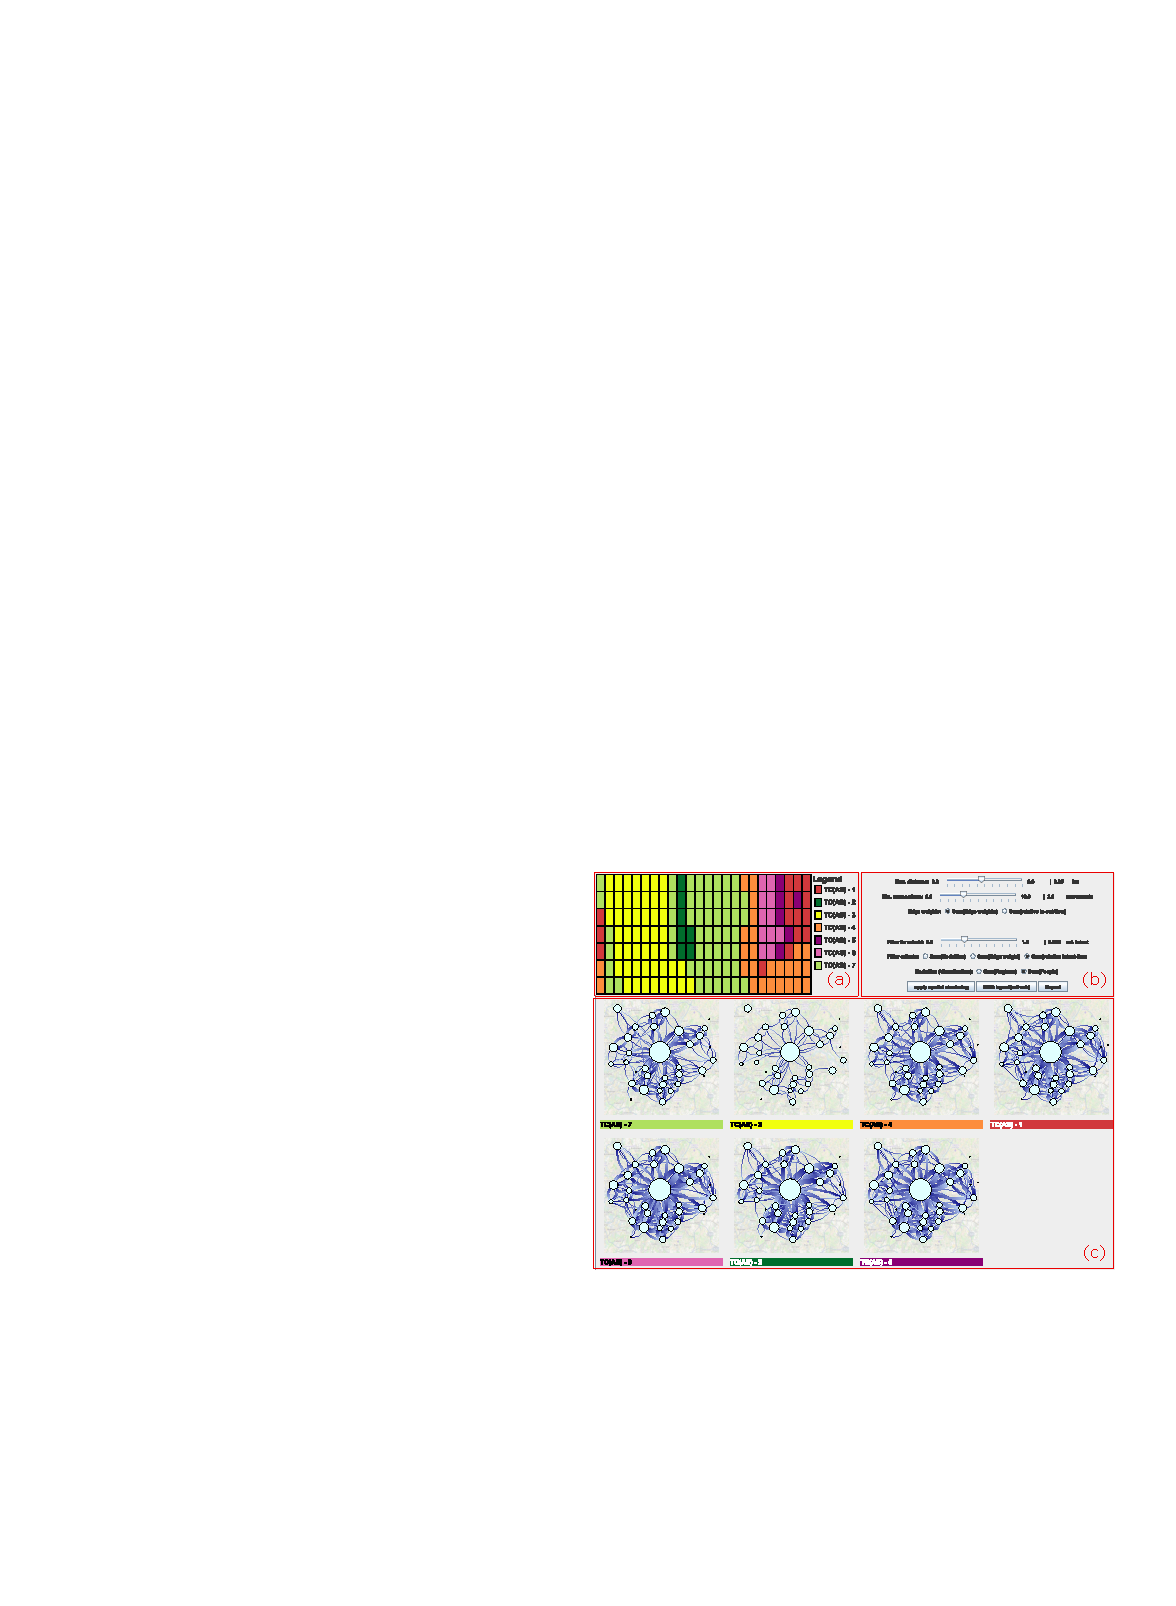
\includegraphics[width=\linewidth]{clus-MobilityGraphs}
	\caption{Temporal clusters of simplified places. \is{Landesberger2016}}
	\label{fig:lr-MobilityGraphs}
\end{figure}

\subsubsection{Classification}
\paragraph{Overview}
Classification predicts the value of a categorical (discrete or nominal) attribute based on the values of other attributes. It builds a model (or \emph{classifier}) based on a labeled training dataset (i.e., \emph{supervised learning}) and applies it in labeling new data~\cite{Han2011}. The model needs to not only identify the labels in the training dataset well but also be general enough to predict the labels of new data correctly. One common and intuitive classification algorithm is decision tree induction~\cite{Quinlan1986}. Each non-leaf node represents a ``test'' on an attribute, which splits the node to multiple branches, each for an outcome of the test. Each leaf node is associated with a class label and is the result of a sequence of tests starting from the root node.

The importance of building a decision tree is choosing which attribute to split at each node. Intuitively, we should choose attributes that can divide nodes into ``pure'' child nodes so that all data items in a child node belong to a single class and no further splits is needed. For example, in a binary classification, consider a training dataset with 10 records, 5 labeled ``true'' and 5 labeled ``false''. Attribute $A1$ splits the set to two subsets: (5 ``true'', 0 ``false'') and (0 ``true'', 5 ``false''). Attribute $A2$ splits the set to (3 ``true'', 2 ``false'') and (2 ``true'', 3 ``false''). The subsets split by $A1$ is ``purer'' than the one by $A2$ because they do not contain a mix of ``true'' and ``false''. To achieve this purity, several attribute measurements have been proposed such as \emph{information gain} and \emph{gini index}~\cite{Tan2006}. More detailed analysis of these measurements and other classification algorithms are out of the scope of this thesis and can be found in data mining textbooks~\cite{Tan2006,Han2011}.

\paragraph{Application Examples}
Exploring a large image collection, such as the set of images available on the Internet, is challenging. Besides the low-level visual features, the semantic contents of images are also effective in searching for relevant ones. Image classification techniques can be used to extract such semantic contents. For example, Fan~et~al.~\cite{Fan2004} detect salient objects in images and associate them with predefined semantic contents according to their perceptual properties. Similar contents are then grouped into a higher level semantic concept; for instance, ``sand field'', ``sea water'' and ``boat'' salient objects construct the concept of ``sea world''. Visualization can help make the output of classification algorithms more interpretable and interactive. To provide an overview of an image collection, Yang~et~al.~\cite{Yang2006} shows the extracted semantic contents, with each as a glyph, in a 2D display so that related contents are located close together using a multidimensional dimension scaling method~\cite{Borg2005}. Similarly, images are also displayed based on their similarity as in \autoref{fig:lr-SIBa}. Zooming and panning are provided to make the visualization more scalable. When an image is selected, the visualization can be switched to a \emph{rainfall} mode, in which the selected image is shown at the bottom and related images are stacked above it based on their similarity with the selected one (\autoref{fig:lr-SIBb}). Users are allowed to reassign the contents computed for each image; however, the model does not take into account the changes to improve its accuracy when classifying new images.

\begin{figure}[!htb]
\centering
\subcaptionbox{Multidimensional dimension scaling view of images.\label{fig:lr-SIBa}}{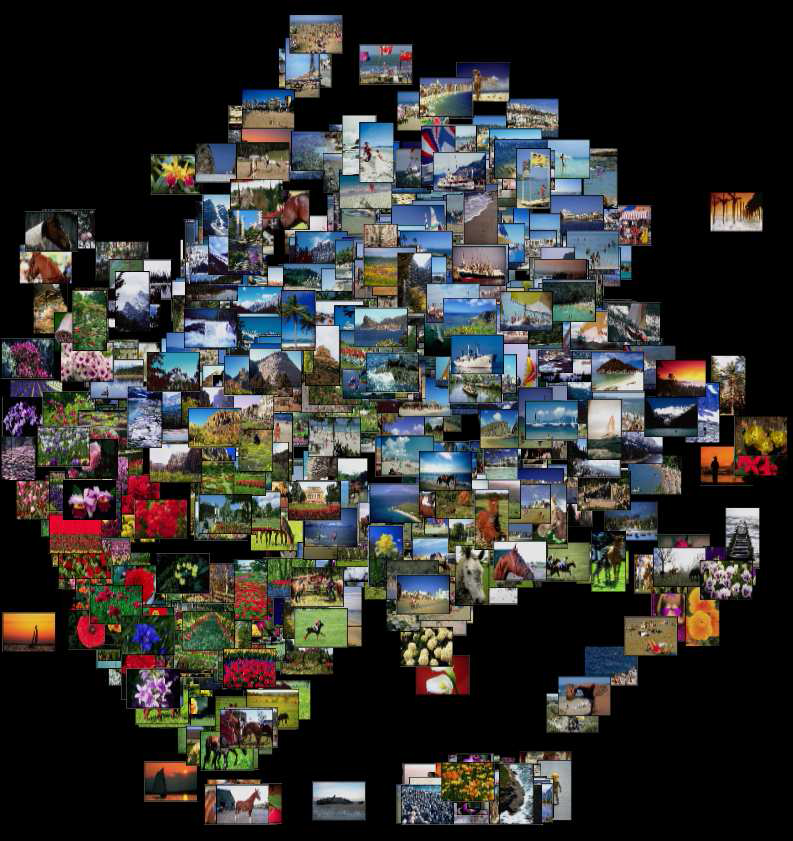
\includegraphics[height=.5\columnwidth]{clas-SIBa}} 
\hfill
\subcaptionbox{Rainfall view of a selected image with highly related images at the bottom.\label{fig:lr-SIBb}}{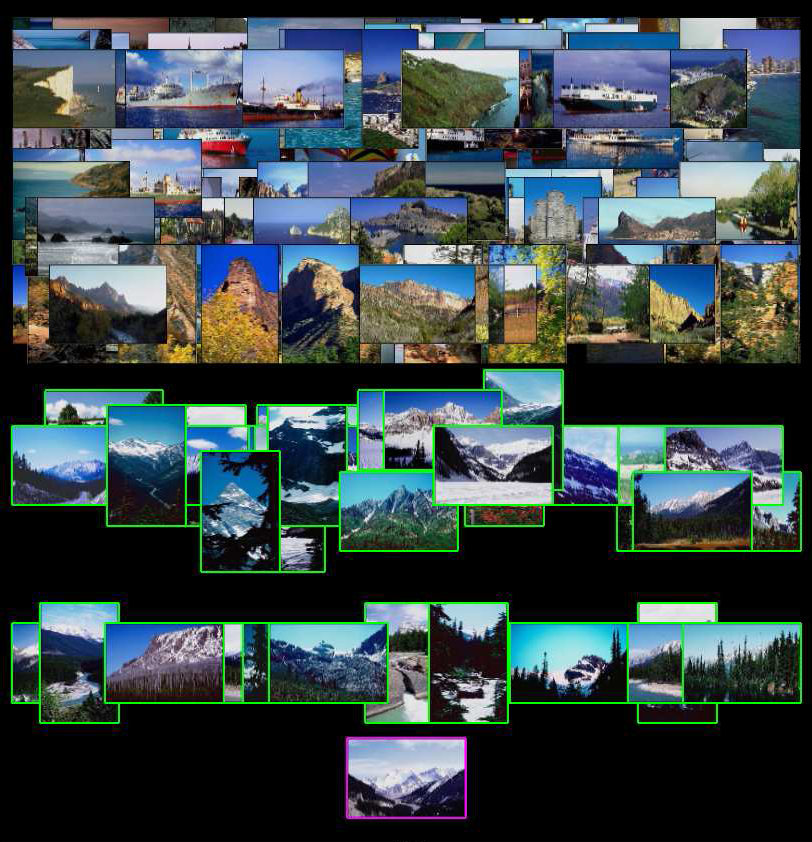
\includegraphics[height=.5\columnwidth]{clas-SIBb}} 
\label{fig:lr-SIB}
\caption{Semantic image browser. \is{Yang2006}}
\end{figure}

In a binary classification, the classifier output is either \emph{positive} or \emph{negative}. Two types of error can happen include \emph{false positive} (classified as positive but the actual class is negative) and \emph{false negative} (classified as negative but the actual class is positive). Depending on a domain, the costs of these error types might be considerably different. For example, wrong prediction of a healthy patient with a cancer has a much lower impact than missing a patient with a real cancer. Migut and Worring~\cite{Migut2010} allow users to adjust the trade-off between these two error types through the visualization of the classification model. Typically, a receiver operating characteristic curve~\cite{Fawcett2006} is used to illustrate the performance of a binary classifier as its discrimination threshold is varied. The curve is composed from a set of true positive rate and false positive rate pairs at various threshold values. Migut and Worring~\cite{Migut2010} replace the true positive rate with the false negative rate (\autoref{fig:lr-Migut1}) because their focus is comparing trade-off between the two error rates. Numerical data is visualized in a scatter plot with the decision boundary separating a 2D plane into two regions, each for a class (\autoref{fig:lr-Migut2}). For each data point, color shows the original class and size indicates the accuracy of the classified class. The current classification setting is shown as a red point on the performance curve, and the user is allowed to move that point along the curve to change the false positive and false negative rates. The classification reruns with the new threshold and rates and updates on the data scatter plot.

\begin{figure}[!htb]
\centering
\subcaptionbox{Performance curve of the classification model with horizontal axis showing the false positive rate and vertical axis showing the false negative rate. rates.\label{fig:lr-Migut1}}[\columnwidth]{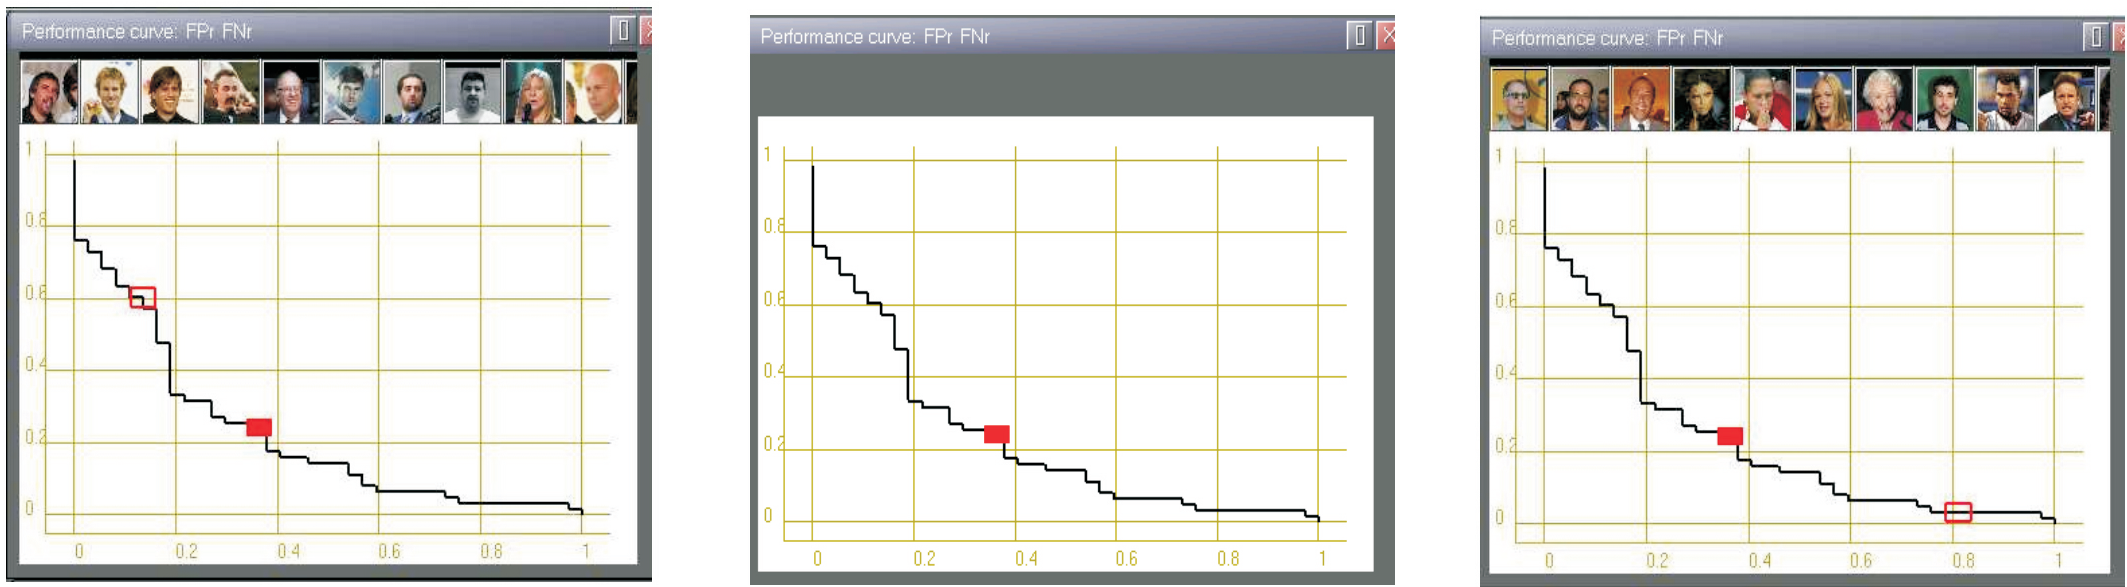
\includegraphics[width=\columnwidth]{clas-Migut1}} 
\\
\subcaptionbox{Data with color indicating original class and size showing classification accuracy.\label{fig:lr-Migut2}}[\columnwidth]{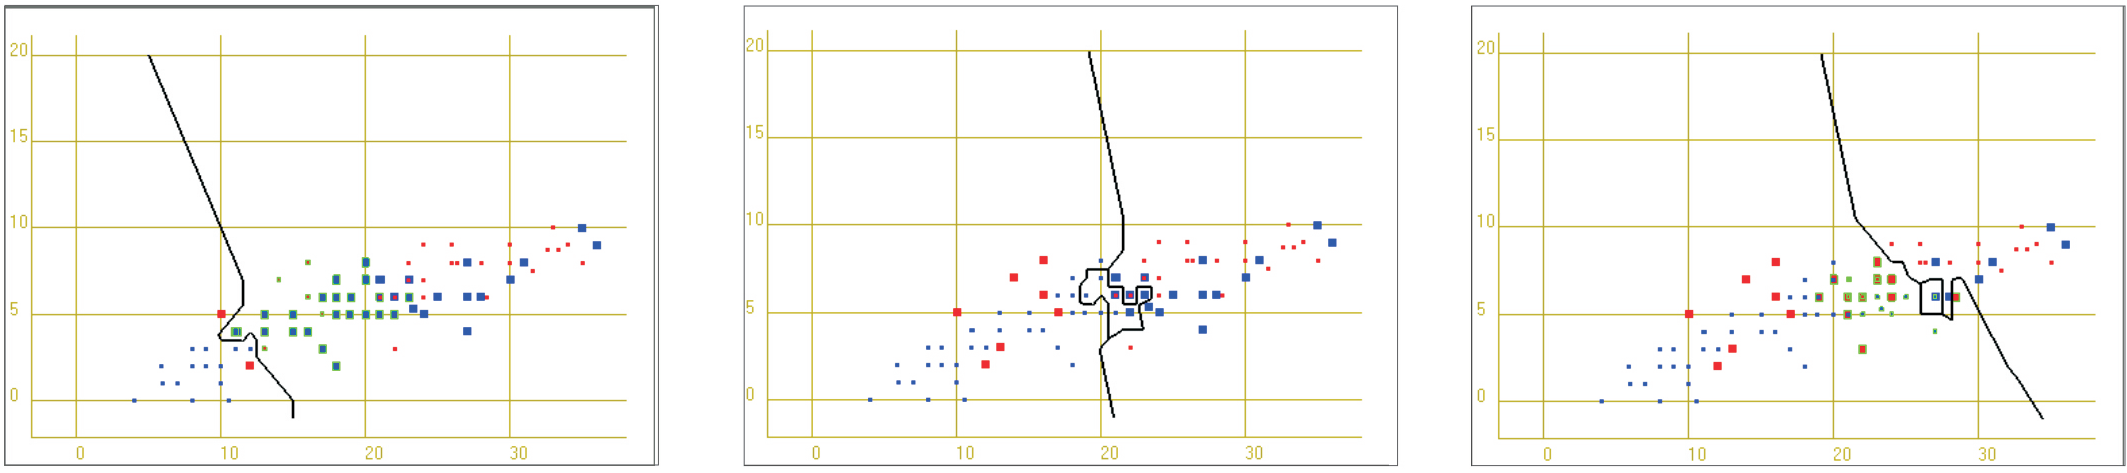
\includegraphics[width=\columnwidth]{clas-Migut2}}
\caption{Visualization and interaction of a classification model. Figure in the middle shows the initial state of the system, with initial operating point on the performance curve and corresponding data scatter plot. Figure on the left shows the state of the system when an expert manipulates the operating point to include more false negatives and on the right to include more false positives. \is{Migut2010}}
\end{figure}

Classification requires training data; however, it can be time-consuming and laborious to produce such a dataset. ScatterBlogs2 includes an interactive classifier that speed up the training data labeling and classifier construction before applying it in real-time monitoring messages of interest~\cite{Bosch2013}. First, the user can search for relevant messages using a standard keyword query. The system then highlights non-trivial terms that frequently co-occur with the original keywords. The result set of highly relevant messages can be used as \emph{positive} samples, whereas some arbitrary messages not returned in the result set can be used as \emph{negative} ones. After creating an initial classifier, the user can inspect messages to correct and update the classifier through the message visualization. Messages are shown in a map as a colored glyph with color hue indicating class and brightness showing classification confidence (\autoref{fig:lr-ScatterBlogs2}). Messages can be filtered by confidence, allowing the user to focus on ones with less certainty, which need human expert to verify. To further speed up the classifier creation, ScatterBlogs2 offers self-training, a technique that iteratively uses messages classified with the highest confidence as labeled data. 

\begin{figure}[!htb]
	\centering
	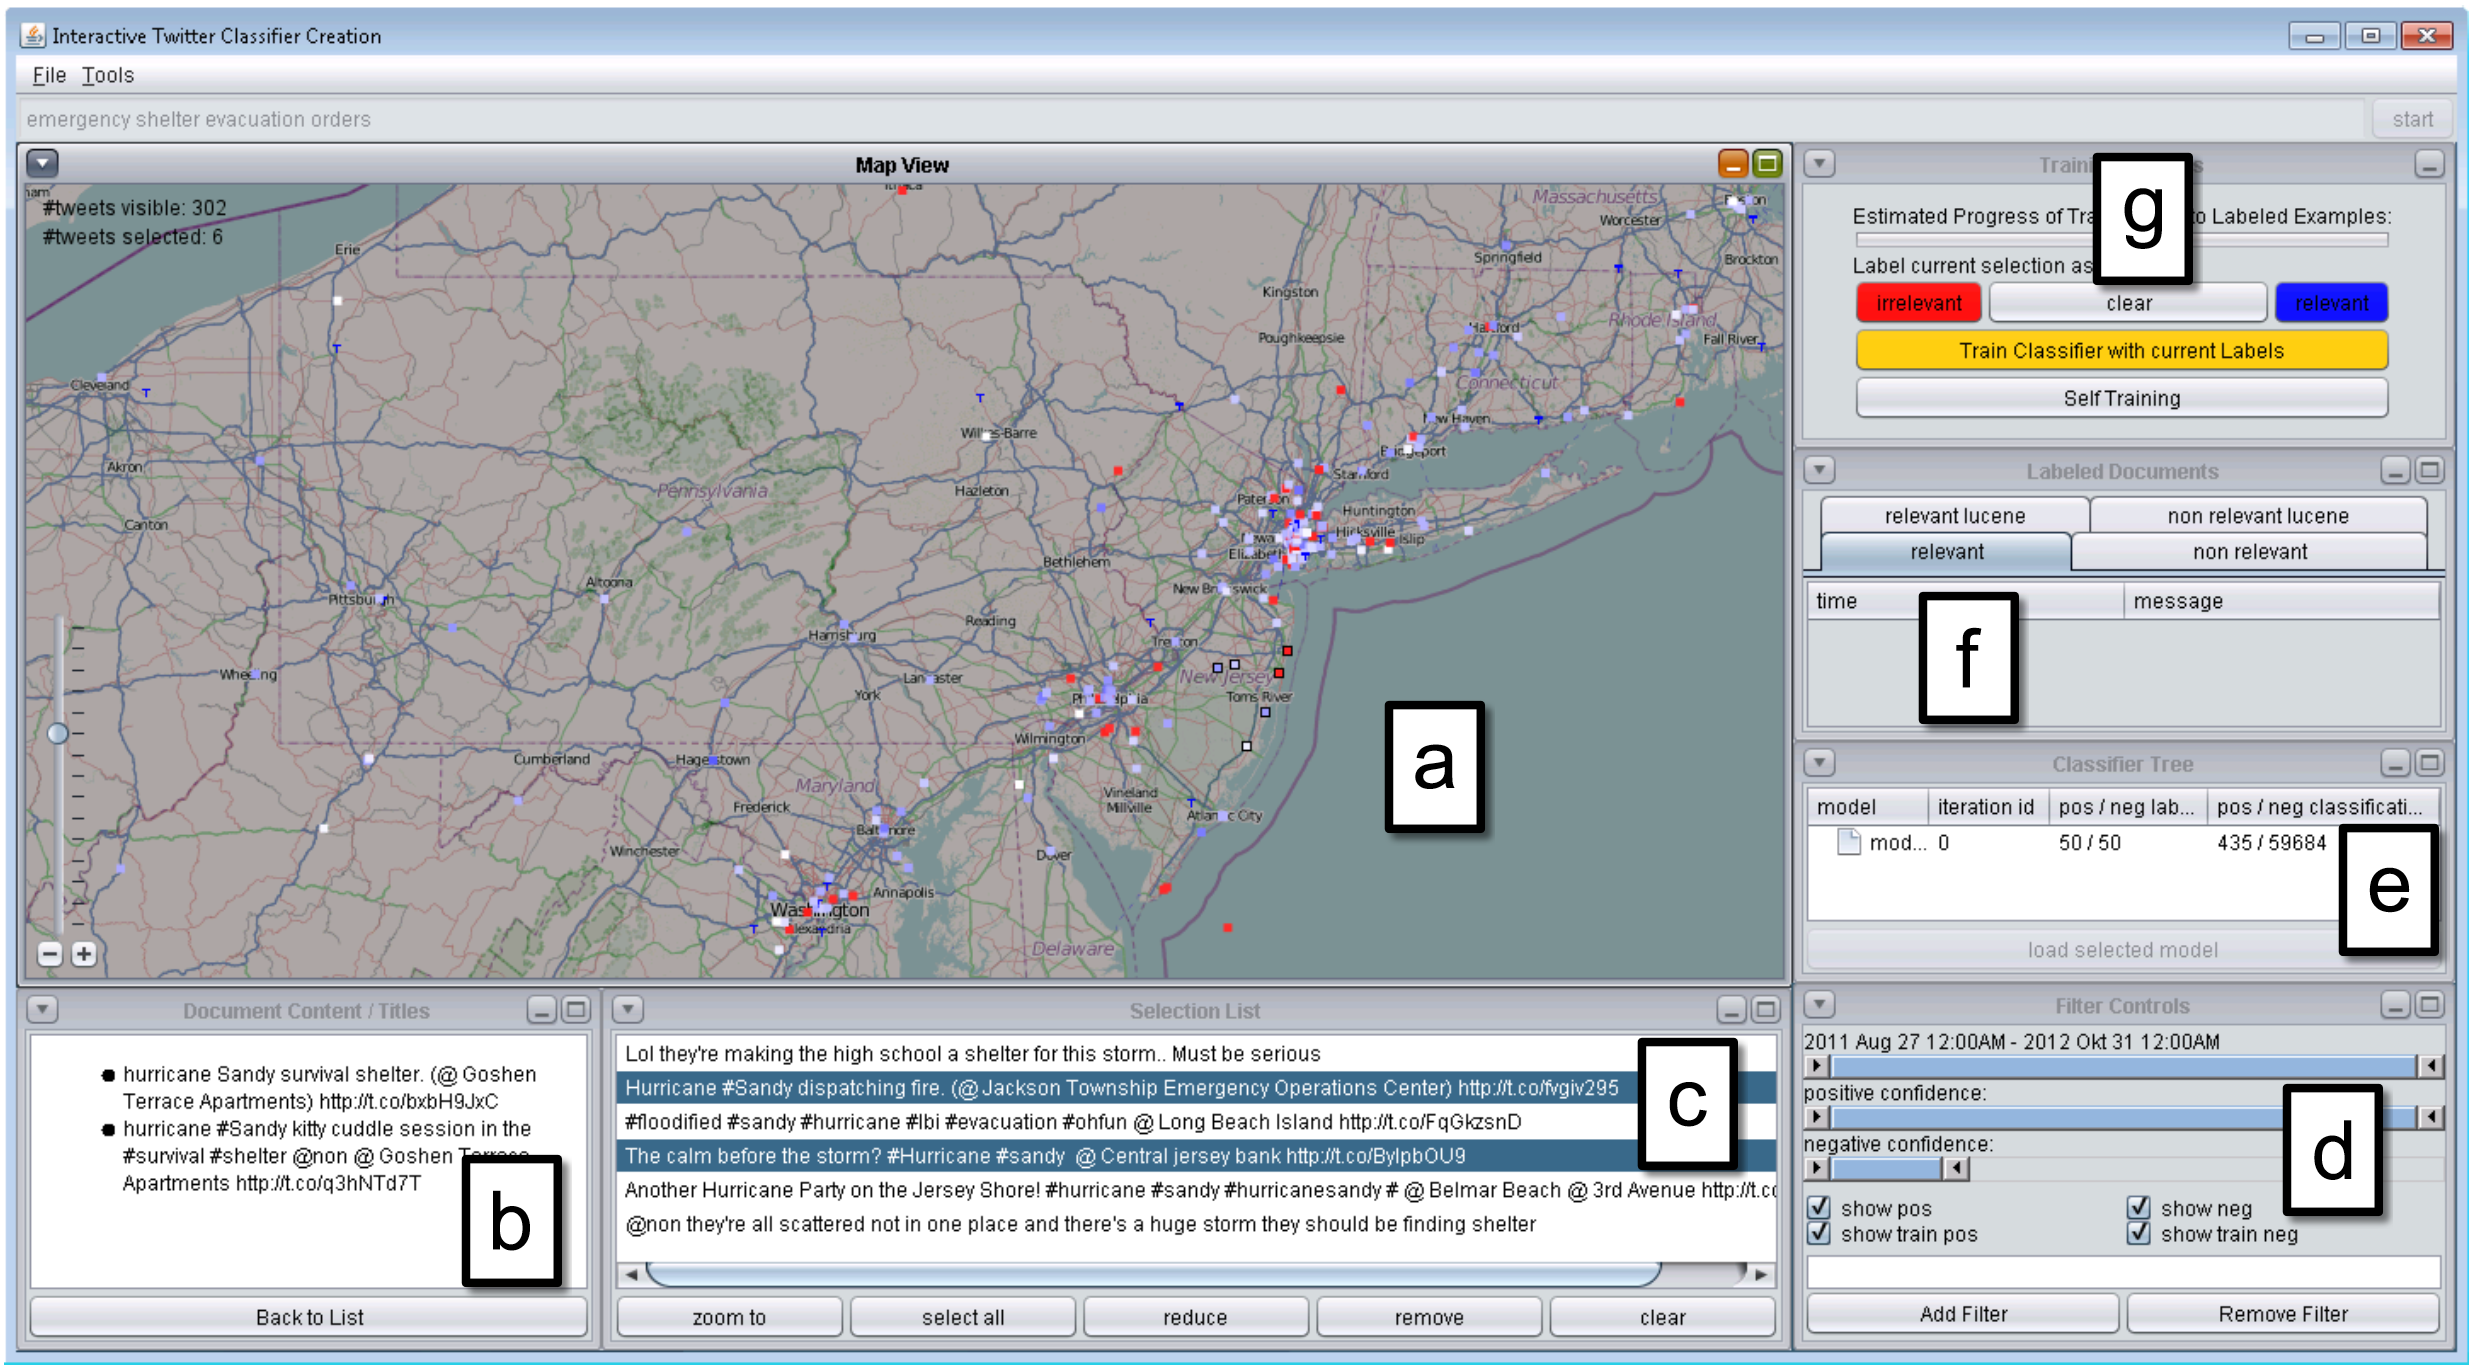
\includegraphics[width=\linewidth]{clas-ScatterBlogs2}
	\caption{The classifier creation environment of ScatterBlogs2. \is{Bosch2013}}
	\label{fig:lr-ScatterBlogs2}
\end{figure}

An essential step in classification of high dimensional datasets is feature selection, which selects a subset of relevant features for use in model construction without much loss of information. This step also simplifies the model and reduces training time. INFUSE~\cite{Krause2014} supports users to explore the predictive power of features in their models. The system allows comparison of features across four feature selection algorithms. Each feature is shown as a circle glyph divided into four equal quadrants, each for an algorithm (\autoref{fig:lr-INFUSE}). A quadrant is further split into 10 slices, each for a cross-validation fold (or random subset of data) to ensure the result  robust. The length of a slice indicates the rank of that feature using a given algorithm. Therefore a glyph can show how its feature performs in different algorithms. To have an overview of all features, INFUSE shows multiple glyphs in either a sequential layout or a scatter plot, where different options can be used for axes such as average rank of a feature or a more sophisticated importance measurement. It also allows users to explore four classification algorithms by showing the score of all 16 combination of feature selection and classification algorithms. More importantly, users are allowed to build their own model by selecting features besides the ones produced by the four given algorithms. The custom feature set is then included in the classification score comparison.

\begin{figure}[!htb]
	\centering
	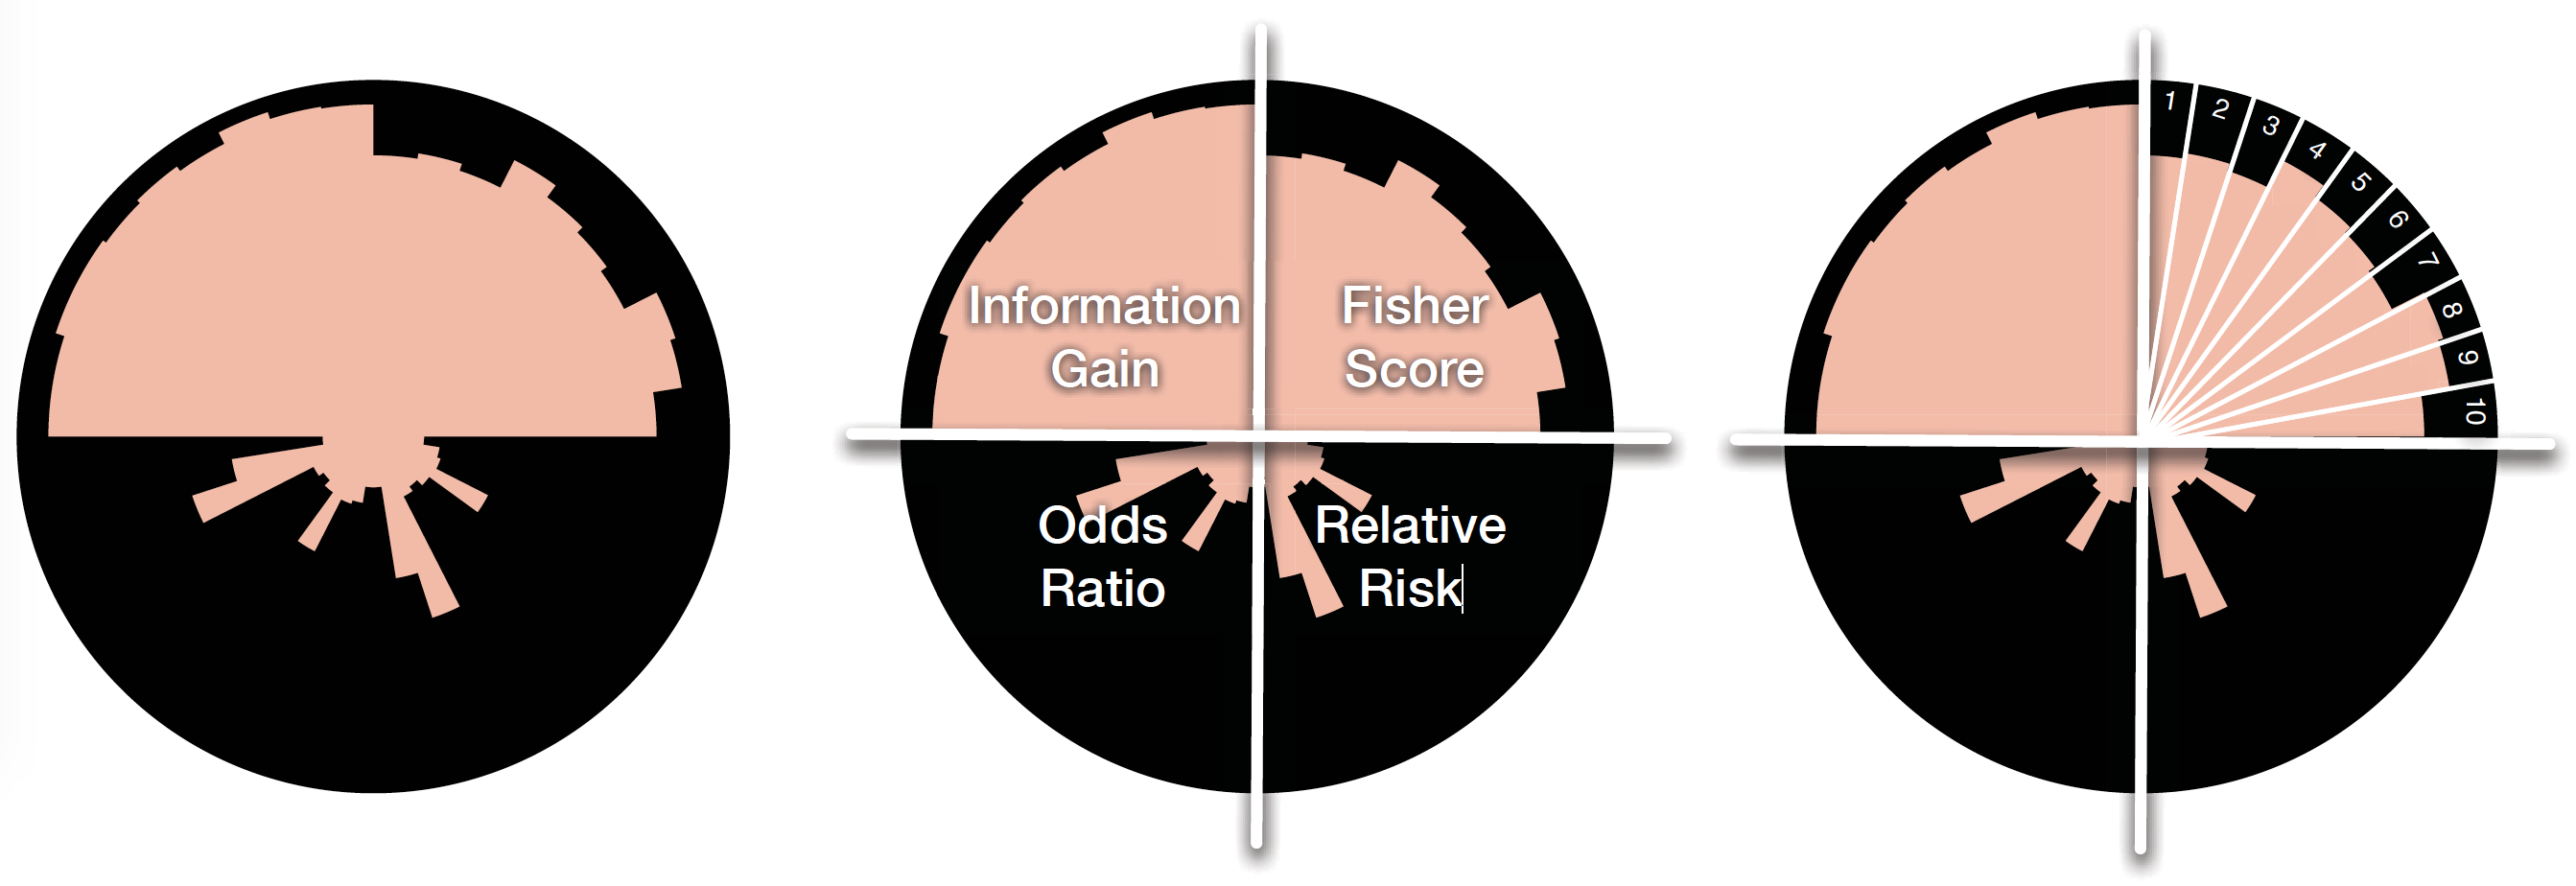
\includegraphics[width=\linewidth]{clas-INFUSE}
	\caption{The feature glyph in INFUSE. \is{Krause2014}}
	\label{fig:lr-INFUSE}
\end{figure}

\subsection{Evaluation Methods}
A visualization, no matter how novel and interesting it is, needs to be evaluated to check whether it meets the design goals and supports the target users to complete the intended tasks. Evaluation has been a research topic in visualization when the field becomes more matured~\cite{Plaisant2004}. Excellent reviews of visualization evaluation with different perspectives include evaluation techniques~\cite{Carpendale2008}, scenarios~\cite{Lam2012} and design process~\cite{Munroe2009}.

In this section, we review the evaluation techniques based on the visualization design model by Munzner~\cite{Munroe2009}, helping address different concerns separately. The four levels include: explain the tasks and available data in the vocabulary of the problem domain, abstract them into domain-independent operations and data types, design visual encoding and interaction techniques to solve the abstract tasks, and develop algorithms to execute these techniques efficiently. Each level has its own \emph{threats} to validity and methods to address them. Two types of methods are distinguished: \emph{immediate} approaches can be done before inner levels are implemented, whereas \emph{downstream} approaches requires all inner levels are completed. The threats and evaluation methods are summarized in \autoref{fig:lr-nested-model}.

\begin{figure}[!htb]
	\centering
	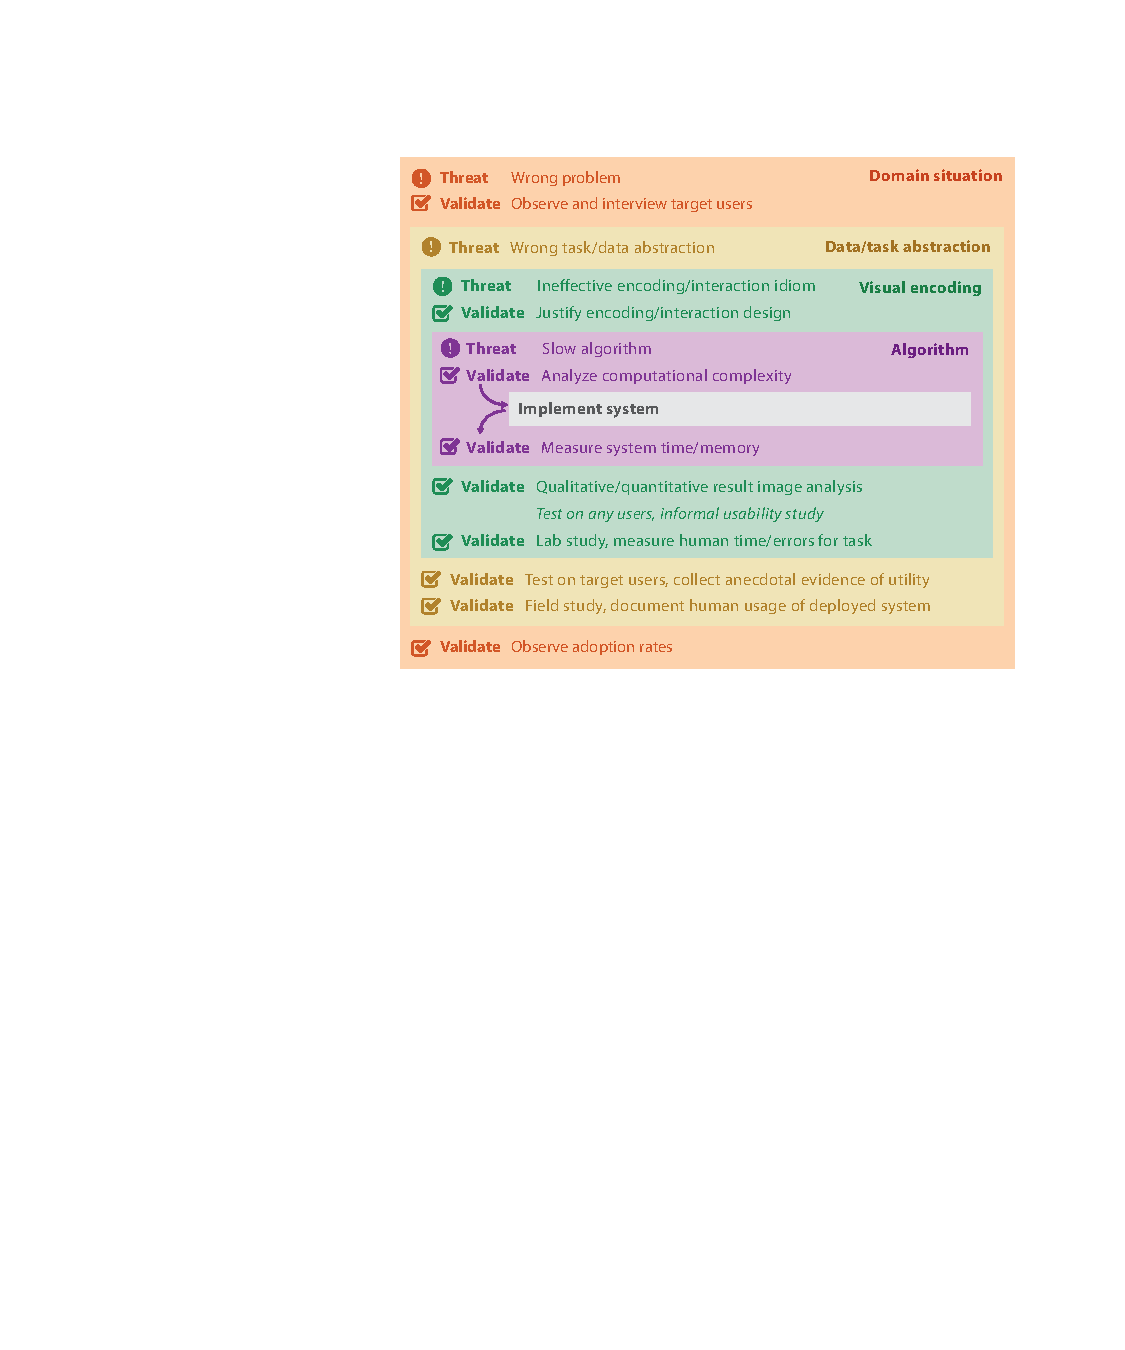
\includegraphics{nested-model}
	\caption{Threats and validation at each of the four nested levels of visualization design. \is{Munzner2014}}
	\label{fig:lr-nested-model}
\end{figure}

\subsubsection{Domain Problem and Data Characterization}
The domain problem of target users is investigated to see if visualization is a potential solution. The primary threat is that the problem is mischaracterized: the users do not really suffer from the identified problem. An immediate form of validation is \emph{field study}~\cite{Carpendale2008}, where the investigator observes how target users act in real-world settings in order to learn and verify the characterization. Another technique is \emph{contextual inquiry}~\cite{Holtzblatt1993}, which allows the investigator to occasionally interview while the user is engaged in the process. One example is the study by Sedlmair~et~al.~\cite{Sedlmair2008} on current working behavior and environments of analysis and diagnosis experts in the automotive industry.

One downstream form of validation is to report the rate the adoption rate of the tool by the target users. High effort is required to make the visualization solution reliable and deployable in the real-world environment. Examples include a field study of Google's Notebook product~\cite{Russell2008} and 6-week field trial of SparTag.us -- a tagging system for foraging web content~\cite{Hong2008}.

\subsubsection{Operation and Data Type Abstraction}
The threat at this level is the identified data and task abstraction do not solve the characterized problem. Only downstream approaches can be used to validate the abstraction. The deployed system needs to be used by target users completing their routine tasks in real-world environment. The goal of this evaluation is to collect anecdotal evidence that the solution is in fact useful. The observation and interview need to focus on understanding how the tool is used, and how it helps or hinders the users in performing their tasks. An example is a longitudinal field study of LiveRAC system that supports analysis of system management time-series data~\cite{McLachlan2008}.

Evaluating the visualizations for supporting sensemaking can be done at this level, as the \emph{evaluating visual data analysis and reasoning} scenario in the taxonomy by Lam~et~al.~\cite{Lam2012}. Due to the nature of sensemaking, evaluation is often carried out as case studies~\cite{Kang2011} with observation and interview, and followed by qualitative data analysis~\cite{Lazar2010}. Attempts also have been made to quantify the insight or knowledge gained during sensemaking~\cite{Wilson2013}.

\subsubsection{Visual Encoding and Interaction Design}
At the design level, the threat is the chosen design is ineffective at communicating the desired abstraction to the user. One immediate form of validation is to justify every design decision based on known design principles such as the ones discussed in \autoref{sub:lr-design}, or more comprehensive predefined guidelines as in heuristic evaluation~\cite{Zuk2006}. Asking experts to review the design prototype also provides valuable feedback~\cite{Tory2005}.

A common downstream approach is to conduct a controlled experiment comparing the design with other state-of-the-art alternatives~\cite{Xu2012}. A number of participants, depending on the  expected size of the experiment, carry out a number of tasks representing real-world cases. Typically, task completion time and accuracy are measured and analyzed using hypothesis testing methods~\cite{Field2003}. Post-task interviews are often combined to establish deeper understanding about how the visualization is used. If the experiment can be completed online, crowd-sourcing approach using Amazon's Mechanical Turk service can help largely increase the size of participants~\cite{Heer2010a}. Another downstream approach is the measurement of common aesthetic metrics such as the number of edge crossings and edge bends that have been used in graph visualization~\cite{Sugiyama1981}.

\subsubsection{Algorithm Design}
The primary threat at this level is the algorithm is suboptimal in terms of time or memory performance. In interactive visualization, it is essential to ensure the interaction responsive in real-time. Analyzing the complexity of the algorithm using the standard approaches from the computer science literature~\cite{Cormen2009} is an intermediate form of validation. The complexity can be computed based on the size of dataset or the display screen. Downstream approaches include measuring running time and memory usage for benchmark datasets.

%http://www.cc.gatech.edu/~stasko/papers/vast09-eval.pdf
%https://www.purdue.edu/discoverypark/vaccine/assets/pdfs/publications/pdf/Beyond%20Usability.pdf
%http://www.cc.gatech.edu/~stasko/7450/Papers/fekete08.pdf
%https://www.cs.ubc.ca/~tmm/courses/cpsc533c-05-fall/readings/vov.pdf
\section{Provenance}
todo: different of data and analytic provenance.Provenance in ordinary context, give examples (food, art)
where?
%must read: very releveant: http://www.cc.gatech.edu/~aendert3/resources/ragan-vast-2015.pdf
\subsection{Data Provenance}
Data provenance research has been taken in different fields, notably scientific workflows and databases. Scientific experiments may consist of thousands of steps, with each step involving distributed data sources and computational data models~\cite{Gil2007}. Workflows have been used to facilitate the assembly, automation and management of such experiments. Notable scientific workflow systems with provenance enabled include Tarvena~\cite{Zhao2008}, Kepler~\cite{Bowers2006} and VisTrails~\cite{Bavoil2005}. Provenance plays an important role in scientific workflows, aiming to support data interpretation, reproduction of experiment results, troubleshooting and optimization~\cite{Miles2007}. The provenance of long and complex workflows is huge, thus pose challenges in storing, querying, and making sense of such data~\cite{Davidson2007}.

Curated databases are populated and updated with a great deal of human effort, typically published on the web~\cite{Buneman2008}. A well-known example is Wikipedia -- a free Internet encyclopedia that allows its users to edit almost any article accessible. Each record in these databases, such as a Wikipedia article, may be edited by many users and referred to other internal and external sources. This produces problems in attribution and provenance: who edited what at when. Research in database provenance can be characterized into a why-where-how framework~\cite{Cheney2007}. \emph{Why}-provenance focuses on the lineage of the output: for each tuple $t$ in the output, the lineage of $t$ is a set of tuples in the input data that helps produce $t$~\cite{Cui2000}. \emph{How}-provenance concerns how the output tuple $t$ is derived from the query~\cite{Green2007}. Finally, \emph{where}-provenance describes specific locations, or cells in relational databases, of the input data that contribute to the query output~\cite{Buneman2001}. To compute these types of provenance, two general approaches have been introduced~\cite{Buneman2008}. An \emph{eager} approach adjusts the query to pass the extra provenance information to the output. Whereas, a \emph{lazy} approach computes provenance on demand.

Data provenance research in scientific workflows and databases has mainly focused on closed systems, which have full access to the data and its provenance. Modern applications with service-oriented~\cite{Papazoglou2007} and cloud-computing~\cite{Buyya2009} architectures bring challenges in tracking and exchanging provenance information across systems. The \emph{Open Provenance Model} is designed to address these challenges~\cite{Moreau2011}. It also supports a digital representation of provenance for any ``thing'', whether produced by computer systems or not. Three types of objects are defined in the model for building this representation. An \emph{artifact} is a state that can be a digital or physical object. A \emph{process} is a series of actions performed on or caused by artifacts, and resulting in new artifacts. An \emph{agent} acts as a catalyst of a process, managing its execution. Different types of causal relationships can be added between these nodes, forming a \emph{provenance graph} as shown in \autoref{fig:lr-provenance-graph}.

\begin{figure}[!htb]
	\centering
	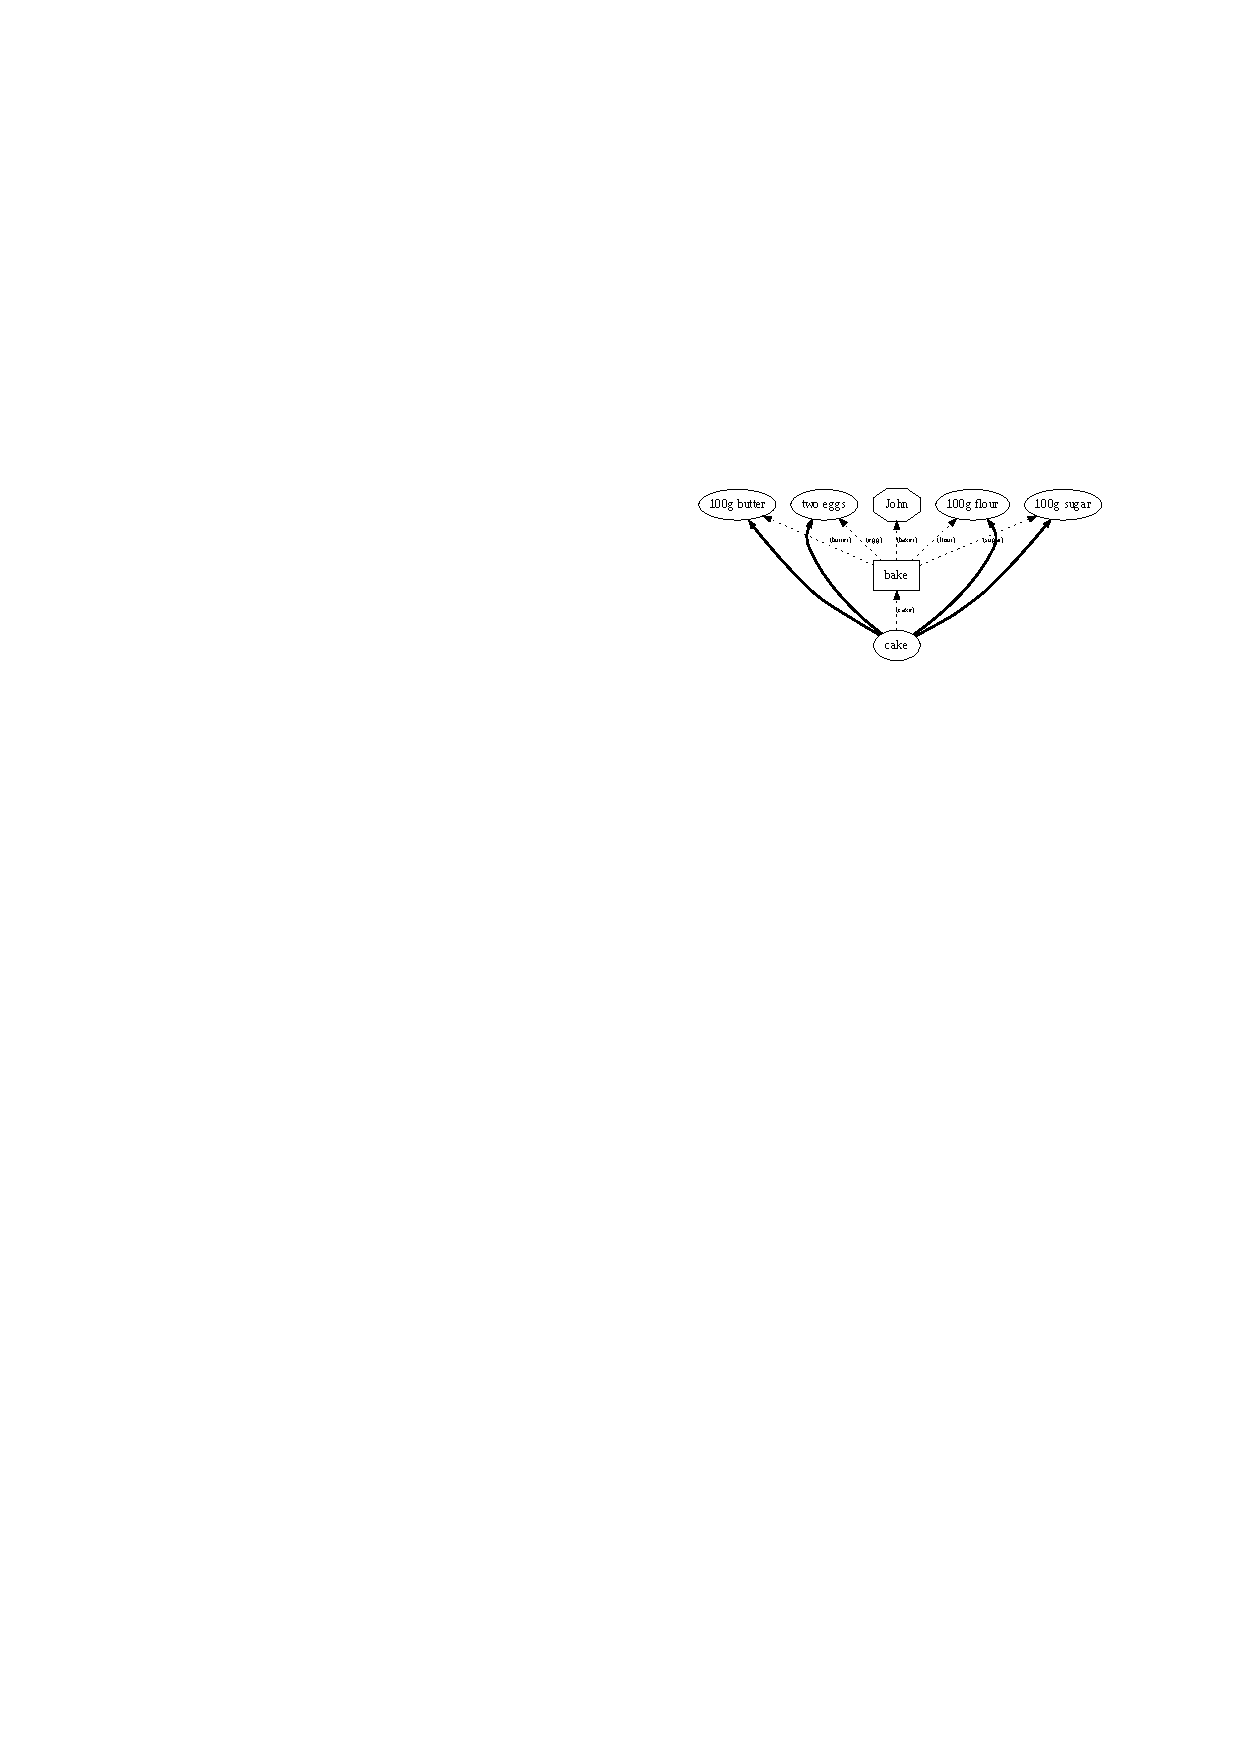
\includegraphics[width=\linewidth]{provenance-graph}
	\caption{A provenance graph for ``cake baking'' using the Open Provenance Model. The cake (artifact) was baked (the process) by John (the agent) using ingredients including butter, eggs, flour and sugar (artifacts). \is{Moreau2011}}
	\label{fig:lr-provenance-graph}
\end{figure}

The Open Provenance Model is general and can be extended in both the structure and vocabulary to represent domain-specific problems. ProveML~\cite{Walker2013} is an extension of this model for recording the provenance of data, analytical process and interpretations in human terrain visual analytics.

\subsection{Analytic Provenance}
Definition from ~\cite{North2011}, our agenda~\cite{Xu2015}

\subsubsection{Model}
Modeling of analytic provenance: 4-level model by Gotz and Zhou and other vis task/action taxonomies such as classic Shneiderman's task by data type~\cite{Shneiderman1996}, Amar's low-level~\cite{Amar2005}, Amar's high-level~\cite{Amar2004}, more recent Bhemer's typology what-why-how~\cite{Brehmer2013}.

\subsubsection{Capture}
combine previous reviews from the draft survey of analytic provenance, research agenda, and capture in the context of online sensenmaking the last paper
%\chapter{Literature Review}

\graphicspath{{Chapter2/figures/}}

- sensemaking
 - some definitions of sm in different contexts
 - PCM
 - DFM
 
- visualization
- analytic provenance
 - capture
 - visualize
 - use
- challenges, gaps in the literature and we're addressing them in this thesis.



 
 \section{Sensemaking}
 Sensemaking is described as the process of comprehension, finding meaning and gaining insight from information, producing new knowledge and informing further action. It has been studied in different contexts such as human-computer interaction~\cite{Russell1993}, information science~\cite{Dervin1983}, and organizational studies~\cite{Weick1995}. Pirolli and Card offer a notional model of sensemaking~\cite{Pirolli2005}, describing a cyclic process involving searching and extracting information, representing it in schemata, manipulating the schemas to form and test hypotheses, then presenting the outcome. Klein et al.~\cite{Klein2006} offer a \textit{data--frame} model describing the interaction of data -- the aspects of the world, and frames -- the accounts of the ``sensemaker'' for the situation. The model consists of a few interconnected iterative processes, each for a certain type of sensemaking activity such as fitting data into a frame.

The notion of sensemaking relates to the way in which human process and interpret information about the world, leading to the creation of new knowledge or insight, which informs further action ~\cite{Pirolli2005}. There are a number of different sensemaking theories, which draw attention from scholars in human-computer interaction, psychology and other areas that consider sensemaking in different contexts. Examples include Dervin~\cite{Dervin1983}, who considers how sensemaking is related to information seeking behaviors and needs, and Weick~\cite{Weick1995}, who was concerned with how sensemaking takes place in organizational settings, from individual and social contexts. Pirolli and Card~\cite{Pirolli2005} offer a notional model of sensemaking, describing a cyclic process involving representations of information in \textit{schemata} and the manipulation of \textit{schemas} to gain insight forming some knowledge or understanding. Klein et al.~\cite{Klein2006} offer the \textit{Data/Frame} theory describing the interaction of \textit{data}, which are aspects of the world and \textit{frames}, that are the sensemaker’s representations of the situation. 

\section{Visualization}
\section{Analytic Provenance}

%\subsection{Timeline Visualization}
% Timeline visualization
%Timeline is one of the earliest visualizations. Back in 1765, Joseph Priestley created the Chart of Biography about two thousand famous people from 1200 B.C to 1750 A.D~\cite{Priestley1765} -- one of the oldest documented timeline. Along a horizontal timeline, Priestley used bars to depict lifespans and dots to illustrate the uncertain birth and dead dates. This remains one of the most popular visual metaphors for timeline visualization: time is represented as a horizontal axis; an event is plotted as a point if it is an instant or a bar spans its interval otherwise. Geographical information can also be included in timeline visualizations as in the classic information visualization example of Napoleon's March on Moscow in 1812-1813 by Charles Joseph Minard~\cite{Minard1869}. 

In this section, we consider related work on representing temporal data and producing timelines, before also examining larger visual analytic systems that include timelines in their feature set.

\subsection{Timeline Visualizations}
% Some examples based on timeline metaphor. Aggregate methods.
A typical example of timeline visualizations is LifeLines~\cite{Plaisant1996a}, a visualization for personal histories, which uses icons to indicate discrete events and thick horizontal lines for continuous ones. When the number of data items is large, they need to be shown collectively rather than individually. The river metaphor~\cite{Havre2002} is one such method that represents thematic changes in large document collections. Storyline visualizations illustrate the dynamic relationships between entities in a story. The technique was first introduced by Munroe with his hand-drawn visualizations~\cite{Munroe2009}. The visualization summarizes movie plots by depicting each character as a line and each interaction between characters as a converging or diverging bundle of those character lines. Computational layouts have since been introduced to automate the rendering process including work by Tanahashi and Ma~\cite{Tanahashi2012} and Liu et al.~\cite{Liu2013}. 

%There are other metaphors to represent temporal data such as the three-dimensional histogram~\cite{Kosara2004}, the spiral graph~\cite{Weber2001}, or calendar-based approaches~\cite{VanWijk1999}. More detail about timelines or more general time-oriented data visualizations can be found in the comprehensive work of Aigner et al.~\cite{Aigner2011}.

% Skip scalability issue because it's not addressed in SchemaLine
%While the time axis metaphor is simple and intuitive, it can be challenging to visualize a large number of events and the relationships among them along a timeline. In the simplest case, all events are unrelated and visualized independently on the timeline. When several events happened during a short period, multiple layers above the timeline need to created to ensure each event's position matches its time point and no two event descriptions overlap~\cite{Plaisant1998,Pioch2006,Andre2007,Liu2010,Kim2010,Munroe2013,SimileTimeline,TimeGlider}. \note[k]{We mentioned timeline scalability here and need to discuss it for SchemaLine} The resulting timeline can quickly get cluttered as events and layers increase. Several attempts have been made to address the scalability issue including semantics zooming with different levels of detail \cite{Andre2007}, focus and context views \cite{Andre2007, SimileTimeline}, and aggregation of multiple events to one single event \cite{Plaisant1998}.

% Visualize relationships between events
Visualizing individual events on a timeline is relatively simple; however, showing relationships between events is quite challenging. One approach is to explicitly draw an edge between two related entities as in tmViewer~\cite{Kumar1998}. Edge styles can be used to depict different kinds of relationships; however, drawing a node-link diagram on top of the timeline can cause the visualization to become cluttered even with a small number of events. Another method is to use the concurrent perception ability of humans by using color coding or icons to indicate different groupings. When events are distributed along the timeline, this method introduces a heavy cognitive load for viewers to scan through the entire timespan. Our method uses colored backgrounds and clusters all events belonging to the same group to reduce user effort. Relationships within multiple faceted temporal data are addressed by Andr\'{e} et al. in Continuum~\cite{Andre2007} by using views with different scales and the classic details-on-demand technique to save space. More recently, SemaTime~\cite{Stab2010} can visualize two different types of relationship: time-dependent (e.g., lives-in) and time-independent (e.g., father-of). SemaTime stacks events vertically and places related events close together. Time-dependent relationships are depicted by using rectangles crossing the relevant common interval of the two events. Time-independent relationships are illustrated by simple arrows.

% Follow events in timeline
%One essential requirement in timeline visualizations is to be able to follow events chronologically. Even though events are aligned with their time, it can still be difficult to trace which events happen after which, especially when they are close. A conventional rule is that an event is preferentially rendered at the bottom. If the representation of the event (normally a short summary of the event) does not overlap with other event representations, it will stay at the bottom; otherwise, it needs to move up a level. In place of this implicit rule, our method creates an explicit path to guide readers, to improve performance in both time and accuracy. 

%Visual attributes, such as colors and font sizes, are commonly used when events have other attributes (such as grouping and importance level) need to be included in the visualization \cite{TimeGlider}. \note[k]{Similarly, we mentioned number of distinguishable colour issue here and need to discuss it for SchemaLine} However, the number of colors that can be easily distinguished is limited, and so are the levels of possible font sizes to ensure legibility and not taking up too much display estate. 

%To address these problems, LifeLines \cite{Plaisant1998} divides the vertical dimension of timeline into multiple stacks, each to represent a group of events. Continuum \cite{Andre2007} represents the hierarchical relationships between events by displaying child events nested in a parent event. For example, in the music context, a piece belongs to a composer, a composer then lives in an era. All pieces of one composer can be displayed inside a bar of the composer, which represents his/her lifespan.

%Events can have additional complex relationships. In genealogical data, there are relationships such as marriage/divorce and parent-child. \note[k]{can reduce the details about this work if need space}{Kim et al. \cite{Kim2010} represent people as individual lines that cover their lifespans. Vertical axis is used to represent relationships. Unrelated people are displayed vertically far enough to indicate that there is no relationship between them. When two persons get married, the two corresponding lines converge into a bundle to indicate a marriage. Whereas, the diverge of a bundle of two lines denote a divorce. The child is visualized close to the bundle of his parents and a vertical faded dash-line is used to connect the beginning of the child line to his parents.} 

%Another example is movie data, in which a scene contains a start time, a duration and members involved. Munroe creates a hand-drawn visualization to summarize characters' interactions in movies, published in the XKCD webcomic ``Movie Narrative Charts'' \cite{Munroe2013}. Inspired from that work, Tanahashi and Ma~\cite{Tanahashi2012} propose a set of design considerations for aesthetic and legible story-line visualizations, and an algorithm to generate visualizations satisfying these design principles. Similar to representing marriage/divorce relationship in genealogical data,  character lines should go straight unless they converge to or diverge from an interaction. The bundle of lines in an interaction should be adjacent; otherwise, lines must be not adjacent to depict separate character lines. To improve the aesthetics and legibility of the visualization, the algorithm also tries to minimize the number of line wiggles (bends), line crossovers, and white space gaps. The visual representation of SchemaLine is inspired by this work. 

%\subsection{Narrative Construction}
%\label{sec:narrative}
%Segel and Heer \cite{Segel2010} reviewed and classified narrative visualizations based on three dimensions: genre, visual narrative tactics, and narrative structure tactics. They define seven (not mutually exclusive) genres of narrative visualizations including magazine style, annotated chart, partitioned poster, flow chart, comic strip, live show, and film/video/animation. Narrative visualizations can also be classified as author-driven, reader-driven, or hybrid. They give an example of a common approach called "Martini Glass Structure". The story begins with the author's guidance for a while and then leads to the reader-driven stage where they can freely explore the story. Among these, most relevant to our work are those designed for sensemaking and utilize a timeline representation.

\subsection{Timelines within Visual Analytics Systems}
A timeline is commonly integrated into Visual Analytics systems designed for making sense of large and complex datasets including POLESTAR~\cite{Pioch2006}, HARVEST~\cite{Gotz2006}, Jigsaw~\cite{Stasko2007, Gorg2013}, and nSpace2 Sandbox~\cite{Wright2006, SandboxTimeline2012}. 

% visualize what?
To support sensemaking, timelines are typically used to visualize not raw data, but more meaningful information such as user notes (POLESTAR, HARVEST) or extracted entities (Jigsaw, nSpace2 Sandbox) instead. HARVEST visualizes both raw data and synthesized knowledge in one timeline to allow progressive investigation. However, filtering must be supported to prevent valuable information getting lost among dense data.

% manipulation of notes
Most of the systems use timelines to show notes statically, to present a known story instead of dynamically discovering a hidden story. nSpace2 Sandbox is an exception -- it allows users to group related entities into sub-timelines and to alter the entity's date on the timeline if needed. However, one entity cannot be added into multiple timelines, which is necessary when an entity's category is uncertain. Our SchemaLine provides a set of fluid interactions to manipulate notes to build a more semantic schema.

% visual representation of notes and schemata
Notes are typically represented using the ``sticky-notes'' metaphor: a colored rectangle as background with text on top of it. nSpace2 Sandbox provides multiple levels of detail for entities: a short summary, a full article, or even entities of entities. Timelines are commonly visualized as a horizontal axis with notes connecting to the timeline by edges. nSpace2 Sandbox uses a vertical axis timeline as the ``diary'' metaphor with columns for sub-timelines.

% layout
POLESTAR requires manual notes arrangement to fit the display. nSpace2 Sandbox uses a simple linear layout to organize entities, thus entities with nearby dates will overlap on the timeline. Our layout algorithm produces an aesthetically pleasing visualization that avoids this issue while still providing easy note manipulation.

% integration
Timelines are often used as an extra view, coordinated with the whole system. Jigsaw provides a reasoning space called Tablet, where a timeline can be added. nSpace2 Sandbox also introduces a separate component called Timeline view. Even though entities from data space can be dropped into timeline space, it may introduce a heavy cognitive load for users to switch between two working spaces. In the evaluation of this paper, we integrate SchemaLine into an existing system seamlessly to provide concurrent exploration and sensemaking with data.

%is a collaborative knowledge management and sense-making tool for intelligence analysts. Users can extract text and take notes when reading documents. Notes are then placed in an empty space to allow analysts to organize and cluster information. This information can be organized in a timeline; however, the user needs to arrange it manually. Without automatic layout and grouping of related information, it is difficult to assist users in sensemaking.
%
%\note[p]{miss 1,3,4}
%HARVEST~\cite{Gotz2006} allows users to interactively define new knowledge when analyzing data. The synthesized information can then be visualized together with raw data on the timeline. This feature could be useful because insight can be progressively used to gain deeper understanding. However, it may cause the findings get lost among dense data; only selective information should be shown on the timeline. The system does not support linking or grouping synthesized knowledge to produce alternative explanations about the case.
%
%\note[p]{miss 3,4,5}
%Jigsaw~\cite{Stasko2007} is one of the most popular Visual Analytics systems for making sense of a large corpus of documents. It can identify various types of entity (people, place, organizations, etc.) within the corpus and present the complex relationships through multiple linked visualizations. Jigsaw also supports a timeline for sensemaking~\cite{Gorg2013} within a feature called ``tablet''. Tablet is an empty canvas, which allows analysts to freely organize information, create links between entities or take notes. When entities are dropped onto the timeline, they will be automatically organized based on their associated date. A disadvantage of the tablet is that the user needs to open another space to enter notes instead of directly inside the data exploration space. The tablet timeline does not support visually showing different groups of related notes, which is quite important when connecting them together to construct a more cohesive explanation. It is also not clear how this timeline is used to support analysis; it is more often used for reporting the story once discovered~\cite{Liu2010}.
%
%\note[p]{miss nothing!!!} \note{maybe we can say how schemaline is different instead?}
%nSpace Sandbox~\cite{Wright2006} is a commercial sensemaking environment that supports extracting information from different sources, organizing it flexibly and linking these pieces of information. Sandbox's timeline~\cite{SandboxTimeline2012} allows the assembly of different types of evidence, such as documents or pictures, along the time axis. It also supports creating \textit{bands} within the timeline to store different groups of events. Relationships between events within bands or within the timeline are visualized by arrows. Sandbox's timeline is quite advanced in terms of analytical features compared to the timelines in other visual analytics systems. However, the simplistic linear timeline layout is not space-efficient and also makes it difficult to visualize close events. Zooming feature is provided to partially address this issue.

%Visualizing documents along a timeline is one of its many features, but it does not directly support group or interactive editing.
%\note[k]{this needs to be updated for later/latest version of GeoTime. Also the focus should be 'timeline' and not 'narrative'} GeoTime \cite{SandboxTimeline2013} is a Visual Analytics system that is designed for the detection of spatial and temporal pattern within the data. It allows annotated visualizations, which can then be used to build a visual narrative. However, the visual narrative is mainly designed for reporting, and there is limited functionalities for the discovery process of the narratives.
%Aruvi~\cite{Shrinivasan2008} is a Visual Analytics system designed to support sensemaking. It allows the creation of notes about any finding and the visualization leads to it. Such notes can be connected to indicate the relationship between them. However, it only provide free-form organization of the notes and there is no support for timeline visualization. 
%HARVEST \cite{Shrinivasan2009} is a Visual Analytics system that adopts a similar approach to sensemaking as the Aruvi. While it uses an algorithm to find relevant discoveries and views for suggestion, there is no significant changes in the support of sensemaking. As a result, it lacks the ability to automatically layout the finding notes or the support for the discovery of any temporal pattern.
%\note[k]{Phong, can you say something about the timeline in 'Sense.us'?} Sense.us \cite{Heer2009} is one of the early attempts of online collaborative visualization. It allows users to annotate visualizations and use them in the collaborative discussion. The trail of annotated visualizations are then used to construct the trail of a topic. This method is useful to record the evolution of the discussions, but it does not indicate the relationships among the discussion, i.e., how they form a narrative, and can make it difficult to understand a large discussion.
\note[p]{I have no idea with timeline in 'i2 analyst notebook'}






\section{Related Work}

\subsection{Timeline Visualizations}
The most common form of timeline visualization uses a horizontal axis to represent time progressing from left to right, with events positioned horizontally according to their timestamps. A well known example is LifeLines~\cite{Plaisant1998} -- a visualization of personal medical records. LifeLines uses icons to indicate discrete events and thick horizontal lines for continuous ones. Timelines can be integrated into a tree format to represent changes in a hierarchy over time as in TimeTree~\cite{Card2006}. Geographical information can also be embedded in timelines as in the classic visualization of Napoleon's March in Moscow in 1812--1813 by Charles Joseph Minard~\cite{Minard1869}. The book by Aigner et al.~\cite{Aigner2011} provides a comprehensive review of timelines and other time-oriented data visualizations.

Techniques such as aggregation and interaction are commonly used when there are a large number of events. LifeLines~\cite{Plaisant1998} aggregates events to save display estate; for example, a series of similar prescriptions can be grouped together. ThemeRiver~\cite{Havre2002} or Streamgraph~\cite{Byron2008} uses a river metaphor to represent aggregated changes of themes over time in a large document collection. Each river is a theme, and its width at certain time points shows the number of documents in that theme. Common interaction techniques are often used in the visualization of large timelines to support their exploration, including overview+detail \cite{Andre2007},  filtering~\cite{Plaisant1996a}, and details-on-demand~\cite{Stab2010}.

\subsection{Set Relations in Timelines}
According to the Gestalt principles of grouping, humans naturally perceive objects as a whole rather than as the sum of their parts~\cite{Koffka1935}. Three of the principles are commonly used to show set relationships among events: similarity, proximity, and uniform connectedness.

The principle of \textit{similarity} states that objects are perceptually grouped together if they are similar to each other~\cite{Koffka1935}. This principle is extensively applied to show set relations in timelines by using colors and shapes. Time indicators as icons (time-point events)~\cite{SimileTimeline2009} and bars (interval events)~\cite{Wang2008} are colored according to event set memberships. Different shapes for icons~\cite{TimeGlider2012} and bars~\cite{Plaisant1998} are also used to distinguish set memberships. It is more challenging to represent multiple set memberships. LineSets~\cite{Alper2011} uses concentric circles for icons, where each circle is colored to represent one set.

According to the \textit{proximity} principle, objects that are close together are perceived to be more related than objects that are spaced further apart~\cite{Koffka1935}. In Chart of Biography~\cite{Priestley1765}, people within a category are placed in a horizontal band, away from people in other categories. LifeLines~\cite{Plaisant1998} splits medical records into different sets, such as \textit{medication} or \textit{diagnosis}, and places them into vertically stacks, which works well if no two sets overlap. Storyline visualizations~\cite{Tanahashi2012,Liu2013} use curved lines to show interactions among characters within the movie timeline. Character lines converge to a bundle if they appear in the same interaction, and diverge when the it ends. Each line can be considered as a set passing through all of its members, and each interaction is a multi-set event. Thus, this method only works for interval events.

Elements tend to be grouped together if they are visually connected~\cite{Palmer1994}. Following this \textit{uniform connectedness} principle, SchemaLine~\cite{Nguyen2014} draws a rectilinear path connecting events belonging to a same set together. Also, tmViewer~\cite{Kumar1998} links related entities with line segments. Different line colors, thicknesses, and styles were used to distinguish set relations. This method can show events with multiple set memberships by connecting them with multiple edges. However, extra edges and crossings may negatively impact the readability of the timeline.

When similarity and proximity are applied together, the later principle dominates~\cite{Ware2013}. Moreover, uniform connectedness is stronger than proximity~\cite{Palmer1994}. For example, objects with different colors and shapes but located close together are more likely to be perceived as a group, and distant objects but with a closed contour surrounding them also provide a strong sense of grouping. Applying these ideas to visualize set relations for timelines, methods relying on similarity such as colored icons~\cite{Wang2008} are less effective than spatial grouping methods such as LifeLines~\cite{Plaisant1996a}. And those, in turn, are less effective than methods using line segments such as tmViewer~\cite{Kumar1998}. 

\subsection{Set Visualizations}
Sets and their relationships can be visualized using Venn~\cite{Ruskey1997} or Euler~\cite{Rodgers2014} diagrams. Simonetto et al.~\cite{Simonetto2009} proposed a technique to automatically visualize sets that were previously not possible with Euler diagrams. However, the complex shapes it produces may reduce visualization readability. In their controlled study, Riche and Dwyer~\cite{Riche2010} showed that for complex set intersections, duplications of shared elements resulted in a better performance in readability tasks than a none-duplicated visualization with more complex shapes. 

These methods assume the positions of set elements are not fixed, which reduces their applicability for geo-located or timeline events. Techniques without such constraints include Bubble Sets~\cite{Collins2009a}, LineSets~\cite{Alper2011}, and KelpFusion~\cite{Meulemans2013}. These methods employ the connectedness principle of the Gestalt laws~\cite{Palmer1994} by connecting set elements using extra visual elements. Bubble Sets draws an iso-contour surrounding elements within a set. This iso-contour is filled with a semi-transparent color so that the intersection between sets is shown as an area of blended color. Collins et al.~\cite{Collins2009a} provided an example of applying Bubble Sets to a timeline, in which case a force-directed algorithm is used to adjust the vertical positions of elements while the horizontal position along the time axis is fixed. 

LineSets applies a B\'{e}zier curve to connect data items. The curve follows the shortest path passing through all elements in the set. Its study showed that LineSets outperforms Bubble Sets in certain readability tasks ~\cite{Alper2011}. KelpFusion, a hybrid technique, uses lines for data-sparse areas and surfaces for data-dense areas. The results of an evaluation on readability tasks~\cite{Meulemans2013} demonstrated that it outperforms Bubble Sets in both accuracy and completion time, and outperforms LineSets in completion time. There has been no reported attempt to apply LineSets or KelpFusion to timeline visualizations. It is expected that crossings between lines, areas and the event text may reduce the timeline readability.







\section{Related Work}

\subsection{Sensemaking and Qualitative Analysis}
Qualitative research methodologies~\cite{adams2008qualititative} are commonly used in study of sensemaking. They allow researchers to reveal often complex user experiences and understand issues that are experienced subjectively or collectively~\cite{Pace2004327, adams2008qualititative}. Moreover, sensemaking research is often concerned not with testing an existing theory, but building a new one through the collection and analysis of relevant data, generating new knowledge about users and the usage of technology~\cite{rogers2012hci}.

There are a number of inductive approaches to qualitative research popular in sensemaking studies, such as \textit{grounded theory}~\cite{corbin1994grounded}, \textit{content analysis}~\cite{stemler2001overview}, and \textit{thematic analysis}~\cite{guest2011applied} that rely on the interpretation of rich textual and multimedia data. There is commonality in these approaches in that they all require a level of manual processing of data, coding and indexing it before describing it in the context of categories or themes. Furthermore, in the case of multimedia data, transcription of audio or video data is often also required. Though these approaches lead to important insights, they are labor intensive, time-consuming and costly in their application \cite{wong2002analysing}. There are a number of widely used software packages which are designed for researches using an inductive approach, offering ways to code and index data in various formats \cite{lewins2007using}. These tools give qualitative researchers useful ways of managing data, however, a qualitative analysis is still a largely manual process which requires a substantial investment of time and resources in leading to insightful findings.

\subsection{Analytic Provenance for Sensemaking}
Analytic provenance describes the interactive data exploration using a visual analytics system and the human sensemaking during that process. Besides the four semantic layers~\cite{Gotz2009} discussed earlier, it also includes the \textit{7W information}~\cite{provenance-7w} (Who, What, Where, Why, When,
Which, and hoW), which were initially proposed for \emph{data provenance}~\cite{data-provenance-survey-sigmod,data-provenance-survey-acm, data-provenance-survey-2008} that focuses on the data collection and computational analysis. This provides the context necessary for interpretation, such as authors, creation time, input data, and visualization parameters. Similar to other scientific workflows, an analytic provenance pipeline consists of capture, storage, analysis and visualization. Heer et al.~\cite{Heer2008} discussed design considerations for such pipeline, which covers underlying provenance's models, visual representations, and operations for analysis. The following discussions focus on the capture and visualization, in the context of recovering of user's sensemaking process from analytic provenance.

\subsubsection{Capture}
There is limited literature on capturing \emph{events} because it is relatively easy and provides little semantics alone. Among these, Glass Box~\cite{Cowley2006} can record a wide range of low-level \textit{events} such as mouse clicks, key strokes, and window events. Its objective is to capture and archive intelligence analysis activities so they can be retrieved later. On a higher semantic level, \textit{Actions}, such as changing the visualization settings and sorting a dataset, are usually performed through interactive widgets including menus and buttons. In theory, it is straightforward to capture them if a visualization system intends to do so. Some systems~\cite{Shrinivasan2008} maintain an action history to support undo and redo, which is an example of utilizing the actions' provenance.

Capturing \textit{task} and \textit{sub-task} is usually more challenging. As previously mentioned, such information is usually part of users' thinking that a visual analytics system does not have direct access to. Existing methods either take a manual or automatic approach. Manual approaches encourage users to record their thinking during sensemaking. However, this will not work if the method introduces considerable distraction or does not offer any benefits. Allowing user annotation is one of the most common forms~\cite{diva,schemaline}: the user creates \emph{notes} or \emph{annotations} that record comments, findings, or hypotheses. Those notes can be associated with the visualization, allowing users returning to the states when the notes were made~\cite{Pike2007, Shrinivasan2008} to re-examine the context or investigate further. The incentive to users is that such annotation digitizes a common sensemaking activity (i.e., note taking) and allows for features such as searching.  This also integrates notes with their visualisation context, allow for better interpretation. However, annotations are unlikely to cover all the analytical thinking. For example, users are more likely to record the findings they made than the process or approach that led them there. To encourage user to write richer notes, a visual analytic system needs to provide additional benefits such as the ability to create visual narratives~\cite{diva} that reveals the reasoning process and help users review and plan exploratory analysis for complex sensemaking task after recording the current progress~\cite{Lunzer2014}.

One of the main disadvantages of manual capture is the requirement of direct input from users. Automatic approaches try to address this by inferring higher level analytic provenance from what can be automatically captured including event and action provenance. However, this turns out to be a difficult task. An experiment studied the effectiveness of manual recovering of reasoning process from a user's action provenance, and the results showed that about 60\% to 70\% of high level analytic provenance can be correctly recovered~\cite{Dou2009}. Given the difficulty, a few methods attempted to partially uncover the high level analytic provenance. One such example is \textit{action chunking}, i.e., identify a group of actions that are likely to be part of the same sub-task, without knowing what the sub-task is~\cite{Gotz2009}. Such approaches apply heuristics to infer patterns from action logs based on repeated occurrence and proximity in data/visualization space or analysis time. More recently, there has been advancement in developing an automated and real-time technique to learn about users~\cite{Brown2014}. Based on very low-level events, mouse clicks and movements, collected from a visual search task, the algorithms can detect whether a user would be fast or slow at completing the task with 62\% to 83\% accuracy. They can also infer some user traits including locus of control, extraversion and neuroticism with 61\% to 67\% accuracy.

Deriving user thinking from their interaction data can be of value beyond understanding sensemaking and is common in other domains. For example, many websites record user browsing interactions in hope to derive higher level information such as user goals and needs. Data mining approaches are commonly used to detect patterns within such data~\cite{Cooley1997}, which can then be used to provide better service such as recommendations~\cite{Wei2007}. Chi et al.~\cite{Chi2001} proposed an algorithm to infer user needs from user's surfing patterns based on the concept of \textit{information scent}, which is the perception of the value and cost of information sources obtained from proximal cues with respect to the goal of the user~\cite{Pirolli1999}.

\subsubsection{Visualization}
Analytic provenance visualization is commonly used to provide an overview of the sensemaking process or reveal any patterns during this process, both of which can help researchers to understand users' thinking. Node-link diagrams are a popular choice to show an overview of the sensemaking process~\cite{vistrails,Pike2007,Shrinivasan2008,Kadivar2009,harvest,Dunne2012}. In most cases, nodes represent system states and edges are actions that transition the system from one state to another. Once an analytic provenance network is created, graph layout algorithms can be applied to improve the visualization. A sensemaking session can have hundreds of system states, and the analytic provenance network usually needs to share the display estate with other visualizations. As a result, it can be challenging to show the entire network within a limited space. It is possible to apply techniques for visualizing large networks such as clustering and aggregation. However, this needs to be done in a way that does not lose the information important for understanding the sensemaking process. To the best of our knowledge, we are not aware of any work addressing this challenge yet.

Besides the overall sensemaking process, the details of each system state and user actions are important for recovery of users' thinking. To provide more context, the common approach is \emph{detail on demand}: when a sensemaking step is selected, the visual analytics system shows the corresponding visualization state and the action's information ~\cite{Pike2007,Shrinivasan2008,Kadivar2009}. This works well if a visual analytics system allows user to go back to a previous state: showing the sensemaking context essentially restores all the visualization views to a previous state. However, to understand a sequence of sensemaking actions, researchers must go through one step at a time, sometimes back and forth. This can introduce extra cognitive work load on the user's memory, thus slow down the analysis. Methods such as GraphTrail~\cite{Dunne2012} show the full details of multiple system states and the links between them at the same time. By zooming and panning, users can choose to see more sensemaking steps (with less detail) or more information about individual system state (but less states simultaneously). This method works well when the visualization state is simple, e.g., only has one view. When a system consists of multiple visualizations, it becomes difficult to see the details of each state when more than one states are shown.

Chronicle~\cite{Grossman2010} utilizes a similar interface to SensePath, but with different design intentions. It captures the entire editing history of a graphical document to allow further study of how a complex image product is accomplished. In contrast, the goal of SensePath is to help analysts recover the high level sensemaking process. Following a similar approach, Delta~\cite{Kong2012} allows comparing different editing workflows to choose the most suitable one by visualizing the steps performed in those workflows. 



\section{Related Work}
Analytic provenance describes the interactive data exploration with a visual analytics system and the human sensemaking during that process~\cite{Xu2015}. Similar to scientific workflows, an analytic provenance pipeline consists of capture, storage, visualization and analysis~\cite{North2011}. Heer et al.~\cite{Heer2008} discuss design considerations for such a pipeline. The following discussions focus on the capture, visualization and utilization in the context of supporting sensemaking.

\subsection{Capture}
Gotz and Zhou~\cite{Gotz2009} divide analytic provenance into four layers according to its semantic richness (in descending order): task, sub-task, action and event. Capturing low level events is relatively straightforward but provides little semantics~\cite{Cowley2006}. Capturing provenance at ``action'' level is more common because it can be done automatically but still provides meaningful information~\cite{Shrinivasan2008, Nguyen2016}. However, capturing ``sub-task'' and ``task'' is more challenging because such information is usually part of users' thinking that systems do not have direct access to~\cite{Gotz2009,Xu2014}.

Brehmer and Munzner~\cite{Brehmer2013} provide a multi-level typology of abstract visualization tasks describing why the task is performed, how the task is
performed, and what are the task’s inputs and outputs. This typology breaks the intention of the user when performing actions into a three-level hierarchy, thus makes it more feasible to capture compared to the high level task and domain-dependent ``task'' and ``sub-task'' in the Gotz and Zhou's model.

% Web: What to collect which can support sensemaking
Information discovered during a browser-based sensemaking task can be collected at different levels of granularity: a web page URL~\cite{Baldonado1997,Gotz2007}, a page element such as \textit{table} and \textit{form} HTML tags~\cite{Schraefel2002,Hong2008}, or a specific fragment of text~\cite{Pioch2006,Nguyen2016}. Finer-grained capture allows users to record what they want with higher precision. Besides this manual capture, visited web pages can be recorded automatically as in browser's history feature. Page linking relationships among pages including opening from a web link and using browser's back button can also be captured~\cite{Ayers1995,Hightower1998,Milic-Frayling2003}.

% Web: Smart way to help collect more
% can remove to save space
%Several methods have developed to help users collect relevant information faster. SenseMaker~\cite{Baldonado1997} allows users to retrieve query results based on similarity with given examples such as web pages having the same domain or articles from co-authors. Dontcheva~et~al~\cite{Dontcheva2006} propose a method to extract similar information by first allowing users to collect a web element, then automatically extracting the information pieces having the same web structure as the collected sample. This method only works with web pages sharing the same template. \note[k]{I don't see any direct connection between sensemaker and Dontcheva's work and sensemap. They appear to be purely algorithmic.} ScratchPad~\cite{Gotz2007} computes and visualizes the relevance between the visiting web page and all the captured information, which may help the user determine the effort needs to spend on the web page.

% Cost structure paper: describe the study here
Besides what to capture, when to capture is also an important decision that needs to be made. Kittur et al~\cite{Kittur2013} conducted a user study to explore when is the best time to ask users to structure the captured information: when all the capture is done or at the same time with the capture. The results show that there are no significant difference between two options in terms of total time spent, cognitive workload, or preference. However, curation at a later stage has significantly better structured data because it has fewer dimensions and these dimensions have more commonalities across participants. 

%Kittur et al~\cite{Kittur2013} conducted a user study to characterize the costs and benefits of curation in the sensemaking process. More specifically, they compared two sensemaking strategies: curation completely after collection or curation at the same time with collection. \annote[k]{Information is collected by highlighting text and curated by assigning a dimension (i.e., tagging) and valence (good/neutral/bad). For instance, ``The Canon EOS Rebel T2i is \textit{good} in terms of \textit{lens}''}{this detail is not necessary}. The results show that there are no significant difference between two options in terms of total time spent, cognitive workload, or preference. However, curation later has significantly better structured data in terms of \annote[k]{fewer dimensions, fewer singleton dimensions, and more commonalities of dimensions across participants}{can you explain this without having to mention the details? It is not obvisou why 'fewer singleton dimensions' is better (or even what it is)}. \annote[k]{We wonder how a hybrid approach, let users curate whenever they want, would perform. We think that curating when collection is done may be adversely affected by the limit of users' working memory, especially with hourly length of sensemaking; and curating immediately after collecting a single piece of information loses the overall picture.}{move this to design discussion.}

\subsection{Visualization}
% Visualization
%In the simplest form, the collected information can be displayed as a list of items, each has a text showing the web page title~\cite{Schraefel2002}, or a table with rows for items and columns for attributes such as page title, URL and abstract~\cite{Baldonado1997}. Hunter--Gatherer~\cite{Schraefel2002} also provides a detailed view showing all collected information pieces together, each consists of a web page title, URL, and the actual captured web element such as text, form, image, and video.

%Tree is another option to organize collected information. SSGIS~\cite{Qu2003} can suggest an initial structure for the search results by clustering them into a tree. POLESTAR~\cite{Pioch2006} allows users to organize the collected snippets into a hierarchy and displays them as in ``Window Explorer''. Dontcheva~et~al~\cite{Dontcheva2006} present ``anchor-based'' layouts to display collected information pieces based on their common anchor attribute. For example, a \textit{calendar} layout can use to organize pieces based on their temporal information; and a \textit{map} layout is suitable to show their spatial information. Timeline is also a common metaphor to display temporal information~\cite{Pioch2006, Nguyen2015}.

Analytic provenance visualization is commonly used to provide an overview of the sensemaking process and to reveal any patterns during this process. Tree visualization is typically used for this purpose~\cite{Pike2007,Kadivar2009,Gotz2010,Dunne2012}. In most cases, a vertex represents a system state and an edge is an action transitioning one state to another. A branch indicates that the user revisits a state and performs another action. A long sensemaking session can produce hundreds of system states, thus makes it more challenging to show the entire process within a limited space. Large network visualization techniques such as clustering and aggregation can be applied to address this issue; however, this should not remove the important information for understanding the sensemaking process. Temporal information can be encoded either by color coded vertex~\cite{Bavoil2005} or edge length~\cite{Shrinivasan2008}. A timeline is also a common metaphor to display temporal information~\cite{Pioch2006, Nguyen2015}.

After understanding the overall sensemaking process, it is common to drill down to examine system states more in-depth. The common approach is \emph{detail on demand}: when a sensemaking step is selected, the visual analytics system allows the user to revisit that state~\cite{Pike2007,Shrinivasan2008,Kadivar2009}. Understanding a sequence of sensemaking actions is more difficult because it requires stepping through all of the actions, sometimes back and forth. This can introduce extra cognitive work load on the user's memory, thus slowing down the analysis. To address this issue, all states can be displayed at once as in Image Graph~\cite{Ma1999} and GraphTrail~\cite{Dunne2012}. However, it worsens the scalability issue.

\subsection{Utilization}
Analytic provenance supports visual narrative construction, during which the user composes findings into a cohesive story. A narrative can include provenance information at different levels: an analysis result, user notes, visualizations and raw data. DIVA~\cite{Walker2013} allows users to create a narrative based on user annotations and captured visualization states, and makes it possible to revisit the visualizations as when they were captured. SchemaLine~\cite{Nguyen2014} enables narrative construction grouping user notes along the timeline.

It is also possible to understand the sensemaking processes of other people by analyzing their analytic provenance~\cite{Dou2010}. SensePath~\cite{Nguyen2016} captures user sensemaking actions and provides a set of visualization and analysis tools allowing other people such as HCI researchers to explore the user sensemaking process through analysis of the captured actions.

% Tagging, node movement, links
%Captured information can be assigned labels or tags to attach meaning and then can be browsed and searched later~\cite{Hong2008, Ryder2010}. This could be a useful starting step in the curation process, which provides the user a semantic structure of the collected information. Other approaches allowing users to create relations among the collected pieces is to freely organize them in the display space~\cite{Pioch2006}  and to draw links connecting related pieces~\cite{Gotz2007}.

% Reasoning
To support further analysis, visual analytics systems commonly provide a ``reasoning workspace'', where the captured information can be freely spatially organized and connected by adding links~\cite{Shrinivasan2008, Xu2014}. Formal analytic methods for reasoning can also be supported. POLESTAR~\cite{Pioch2006} uses a graphical approach to support Toulmin argumentation~\cite{Toulmin2003}: it represents arguments as a tree structure of supporting/rebutting claims, each powered by at least one piece of evidence. Sandbox~\cite{Wright2006} supports analysis of competing hypotheses by assigning each supporting/counter evidence of all the hypotheses a score based on its relevance  and computing the final score to support user decision making.

% Presentation/Organization/Story-telling
After solving a sensemaking task, users may need to present their findings; for instance, to their colleagues to share the knowledge or to their managers as part of the report. They may also need to customize their story depending on different audience's needs and backgrounds. Sandbox~\cite{Wright2006} generates a report by simply exporting curated collections to HTML. Diigo~\footnote{\url{https://www.diigo.com/}}, an online bookmarking tool, allows the user to combine the collected information with their own notes to produce a more organized document with supporting information.

% Share: too trivial?
%Another common way to communicate the findings is through sharing. A (curated) collection can be exported as a local file~\cite{Dontcheva2006} or an online URL~\cite{Schraefel2002}. Social bookmarking also allows users to collect information but considers sharing to community in the first place.\note[k]{I dont' understand} Delicious~\footnote{\url{http://delicious.com/}} is one of the earliest bookmarking services allowing users to save and share web pages of interest and categorize them by tagging. It also attracts attention from academics such as discussing design principles for a social bookmarking service in a large enterprise addressing online identity, privacy and information discovery issues~\cite{Millen2006}. \note[k]{why is this relevant?}

%\chapter{SchemaLine}

\graphicspath{{Chapter3/figures/}}

Timeline visualization is an important tool for sensemaking. It allows analysts to examine information in chronological order and to identify temporal patterns and relationships. However, many existing timeline visualization methods are not designed for the dynamic and iterative nature of the sensemaking process and the various analysis activities it involves. In this paper, we introduce a novel timeline visualization, SchemaLine, to address these deficiencies. SchemaLine is designed to group notes into analyst-determined schema, using a layout algorithm to produce compact but aesthetically pleasing timeline visualization, and includes fluid user interactions to support sensemaking activities. It enables interactive temporal schemata construction with seamless integration with visual data exploration and note taking. Our preliminary evaluation results show that the participants found the new method easy to learn and use, and its features effective for the sensemaking activities for which it was designed.

\section{Introduction}
Intelligence analysis is defined as ``the application of individual and collective cognitive methods to weigh data and test hypotheses within a secret socio-cultural context''~\cite{Johnston2005}. To gain a deeper understanding into the sensemaking process in intelligence analysis, Pirolli and Card~\cite{Pirolli2005} conducted a cognitive task analysis with analysts and proposed a process model of sensemaking, which was described earlier in detail in \autoref{sub:lr-sensemaking}. During the sensemaking process, analysts need to read thousands of reports and extract relevant details, organize them in a way that help the analysts to identify patterns and generate hypotheses. This is challenging because of the large number of documents involved and the complex relationship of entities discovered. Visual analytics systems~\cite{Pioch2006,Wright2006,Stasko2007} facilitate intelligence analysis with automated techniques applied to leverage manual investigation of a large document collection. For instance, named-entity recognition techniques~\cite{Nadeau2007} can identify entities (i.e., persons, organizations and locations), and topic modeling techniques~\cite{Blei2003} can extract the main themes discussed. To help analysts manage a large number of discoveries they made during the sensemaking process, the systems allow them to externalize their thoughts through note taking. Analysts are then often supported to freely organized their notes in a way that makes sense to them and facilitates their analyses, such as constructing a timeline of suspicious events.

% Problem of exisiting timelines in sensemaking
\emph{Timeline} is a simple yet powerful technique to visualize time-oriented data~\cite{Tufte1983}, allowing exploration and identification of temporal patterns and relationships in the data. It displays events along the time axis and position them at the time points at which they occur or the time ranges over which they last~\cite{Plaisant1996}. Timelines have been applied extensively in visualizing both raw data and analysis findings for supporting sensemaking. POLESTAR~\cite{Pioch2006} and HARVEST~\cite{Gotz2006} allow analysts to take notes, define new knowledge, and explore them through a timeline visualization. Jigsaw~\cite{Gorg2013} uses timelines to organize extracted named entities, one for each type. Similarly, nSpace2 Sandbox~\cite{SandboxTimeline2012} provides the creation of multiple sub-timelines for visualizing different types of artifacts. However, these timeline visualizations either lack an automatic layout~\cite{Pioch2006} or use an overly-simplistic linear layout~\cite{SandboxTimeline2012}. As a result, the visualization requires significant effort from analysts to manually arrange data elements, making it difficult to detect temporal patterns.

Sensemaking includes dynamic activities centering around the collected data and its explanation~\cite{Klein2003}. Therefore, to support the dynamic nature of sensemaking, timeline visualizations should allow analysts to create and edit temporal structures interactively. Also, the interaction should be intuitive and fluid~\cite{Elmqvist2011} to prevent analysts from extra cognitive effort and distraction. However, existing timeline visualization techniques are mainly designed for presenting a known story rather than revealing and constructing a hidden one interactively.

In this chapter, we introduce a novel timeline visualization -- SchemaLine -- to address the aforementioned issues. More specifically, SchemaLine contributes
\begin{itemize}
	\item A visual design for an interactive timeline that groups annotations into user-determined schemas.
	\item A compact and aesthetically pleasing timeline layout.
	\item A set of fluid interactions with the timeline to support the sensemaking activities described in the Data--Frame model~\cite{Klein2003}.
\end{itemize}
%\section{Related Work}
\label{sec:relatedwork}

%\subsection{Timeline Visualization}
% Timeline visualization
%Timeline is one of the earliest visualizations. Back in 1765, Joseph Priestley created the Chart of Biography about two thousand famous people from 1200 B.C to 1750 A.D~\cite{Priestley1765} -- one of the oldest documented timeline. Along a horizontal timeline, Priestley used bars to depict lifespans and dots to illustrate the uncertain birth and dead dates. This remains one of the most popular visual metaphors for timeline visualization: time is represented as a horizontal axis; an event is plotted as a point if it is an instant or a bar spans its interval otherwise. Geographical information can also be included in timeline visualizations as in the classic information visualization example of Napoleon's March on Moscow in 1812-1813 by Charles Joseph Minard~\cite{Minard1869}. 

In this section, we consider related work on representing temporal data and producing timelines, before also examining larger visual analytic systems that include timelines in their feature set.

\subsection{Timeline Visualizations}
% Some examples based on timeline metaphor. Aggregate methods.
A typical example of timeline visualizations is LifeLines~\cite{Plaisant1996a}, a visualization for personal histories, which uses icons to indicate discrete events and thick horizontal lines for continuous ones. When the number of data items is large, they need to be shown collectively rather than individually. The river metaphor~\cite{Havre2002} is one such method that represents thematic changes in large document collections. Storyline visualizations illustrate the dynamic relationships between entities in a story. The technique was first introduced by Munroe with his hand-drawn visualizations~\cite{Munroe2009}. The visualization summarizes movie plots by depicting each character as a line and each interaction between characters as a converging or diverging bundle of those character lines. Computational layouts have since been introduced to automate the rendering process including work by Tanahashi and Ma~\cite{Tanahashi2012} and Liu et al.~\cite{Liu2013}. 

%There are other metaphors to represent temporal data such as the three-dimensional histogram~\cite{Kosara2004}, the spiral graph~\cite{Weber2001}, or calendar-based approaches~\cite{VanWijk1999}. More detail about timelines or more general time-oriented data visualizations can be found in the comprehensive work of Aigner et al.~\cite{Aigner2011}.

% Skip scalability issue because it's not addressed in SchemaLine
%While the time axis metaphor is simple and intuitive, it can be challenging to visualize a large number of events and the relationships among them along a timeline. In the simplest case, all events are unrelated and visualized independently on the timeline. When several events happened during a short period, multiple layers above the timeline need to created to ensure each event's position matches its time point and no two event descriptions overlap~\cite{Plaisant1998,Pioch2006,Andre2007,Liu2010,Kim2010,Munroe2013,SimileTimeline,TimeGlider}. \note[k]{We mentioned timeline scalability here and need to discuss it for SchemaLine} The resulting timeline can quickly get cluttered as events and layers increase. Several attempts have been made to address the scalability issue including semantics zooming with different levels of detail \cite{Andre2007}, focus and context views \cite{Andre2007, SimileTimeline}, and aggregation of multiple events to one single event \cite{Plaisant1998}.

% Visualize relationships between events
Visualizing individual events on a timeline is relatively simple; however, showing relationships between events is quite challenging. One approach is to explicitly draw an edge between two related entities as in tmViewer~\cite{Kumar1998}. Edge styles can be used to depict different kinds of relationships; however, drawing a node-link diagram on top of the timeline can cause the visualization to become cluttered even with a small number of events. Another method is to use the concurrent perception ability of humans by using color coding or icons to indicate different groupings. When events are distributed along the timeline, this method introduces a heavy cognitive load for viewers to scan through the entire timespan. Our method uses colored backgrounds and clusters all events belonging to the same group to reduce user effort. Relationships within multiple faceted temporal data are addressed by Andr\'{e} et al. in Continuum~\cite{Andre2007} by using views with different scales and the classic details-on-demand technique to save space. More recently, SemaTime~\cite{Stab2010} can visualize two different types of relationship: time-dependent (e.g., lives-in) and time-independent (e.g., father-of). SemaTime stacks events vertically and places related events close together. Time-dependent relationships are depicted by using rectangles crossing the relevant common interval of the two events. Time-independent relationships are illustrated by simple arrows.

% Follow events in timeline
%One essential requirement in timeline visualizations is to be able to follow events chronologically. Even though events are aligned with their time, it can still be difficult to trace which events happen after which, especially when they are close. A conventional rule is that an event is preferentially rendered at the bottom. If the representation of the event (normally a short summary of the event) does not overlap with other event representations, it will stay at the bottom; otherwise, it needs to move up a level. In place of this implicit rule, our method creates an explicit path to guide readers, to improve performance in both time and accuracy. 

%Visual attributes, such as colors and font sizes, are commonly used when events have other attributes (such as grouping and importance level) need to be included in the visualization \cite{TimeGlider}. \note[k]{Similarly, we mentioned number of distinguishable colour issue here and need to discuss it for SchemaLine} However, the number of colors that can be easily distinguished is limited, and so are the levels of possible font sizes to ensure legibility and not taking up too much display estate. 

%To address these problems, LifeLines \cite{Plaisant1998} divides the vertical dimension of timeline into multiple stacks, each to represent a group of events. Continuum \cite{Andre2007} represents the hierarchical relationships between events by displaying child events nested in a parent event. For example, in the music context, a piece belongs to a composer, a composer then lives in an era. All pieces of one composer can be displayed inside a bar of the composer, which represents his/her lifespan.

%Events can have additional complex relationships. In genealogical data, there are relationships such as marriage/divorce and parent-child. \note[k]{can reduce the details about this work if need space}{Kim et al. \cite{Kim2010} represent people as individual lines that cover their lifespans. Vertical axis is used to represent relationships. Unrelated people are displayed vertically far enough to indicate that there is no relationship between them. When two persons get married, the two corresponding lines converge into a bundle to indicate a marriage. Whereas, the diverge of a bundle of two lines denote a divorce. The child is visualized close to the bundle of his parents and a vertical faded dash-line is used to connect the beginning of the child line to his parents.} 

%Another example is movie data, in which a scene contains a start time, a duration and members involved. Munroe creates a hand-drawn visualization to summarize characters' interactions in movies, published in the XKCD webcomic ``Movie Narrative Charts'' \cite{Munroe2013}. Inspired from that work, Tanahashi and Ma~\cite{Tanahashi2012} propose a set of design considerations for aesthetic and legible story-line visualizations, and an algorithm to generate visualizations satisfying these design principles. Similar to representing marriage/divorce relationship in genealogical data,  character lines should go straight unless they converge to or diverge from an interaction. The bundle of lines in an interaction should be adjacent; otherwise, lines must be not adjacent to depict separate character lines. To improve the aesthetics and legibility of the visualization, the algorithm also tries to minimize the number of line wiggles (bends), line crossovers, and white space gaps. The visual representation of SchemaLine is inspired by this work. 

%\subsection{Narrative Construction}
%\label{sec:narrative}
%Segel and Heer \cite{Segel2010} reviewed and classified narrative visualizations based on three dimensions: genre, visual narrative tactics, and narrative structure tactics. They define seven (not mutually exclusive) genres of narrative visualizations including magazine style, annotated chart, partitioned poster, flow chart, comic strip, live show, and film/video/animation. Narrative visualizations can also be classified as author-driven, reader-driven, or hybrid. They give an example of a common approach called "Martini Glass Structure". The story begins with the author's guidance for a while and then leads to the reader-driven stage where they can freely explore the story. Among these, most relevant to our work are those designed for sensemaking and utilize a timeline representation.

\subsection{Timelines within Visual Analytics Systems}
A timeline is commonly integrated into Visual Analytics systems designed for making sense of large and complex datasets including POLESTAR~\cite{Pioch2006}, HARVEST~\cite{Gotz2006}, Jigsaw~\cite{Stasko2007, Gorg2013}, and nSpace2 Sandbox~\cite{Wright2006, SandboxTimeline2012}. 

% visualize what?
To support sensemaking, timelines are typically used to visualize not raw data, but more meaningful information such as user notes (POLESTAR, HARVEST) or extracted entities (Jigsaw, nSpace2 Sandbox) instead. HARVEST visualizes both raw data and synthesized knowledge in one timeline to allow progressive investigation. However, filtering must be supported to prevent valuable information getting lost among dense data.

% manipulation of notes
Most of the systems use timelines to show notes statically, to present a known story instead of dynamically discovering a hidden story. nSpace2 Sandbox is an exception -- it allows users to group related entities into sub-timelines and to alter the entity's date on the timeline if needed. However, one entity cannot be added into multiple timelines, which is necessary when an entity's category is uncertain. Our SchemaLine provides a set of fluid interactions to manipulate notes to build a more semantic schema.

% visual representation of notes and schemata
Notes are typically represented using the ``sticky-notes'' metaphor: a colored rectangle as background with text on top of it. nSpace2 Sandbox provides multiple levels of detail for entities: a short summary, a full article, or even entities of entities. Timelines are commonly visualized as a horizontal axis with notes connecting to the timeline by edges. nSpace2 Sandbox uses a vertical axis timeline as the ``diary'' metaphor with columns for sub-timelines.

% layout
POLESTAR requires manual notes arrangement to fit the display. nSpace2 Sandbox uses a simple linear layout to organize entities, thus entities with nearby dates will overlap on the timeline. Our layout algorithm produces an aesthetically pleasing visualization that avoids this issue while still providing easy note manipulation.

% integration
Timelines are often used as an extra view, coordinated with the whole system. Jigsaw provides a reasoning space called Tablet, where a timeline can be added. nSpace2 Sandbox also introduces a separate component called Timeline view. Even though entities from data space can be dropped into timeline space, it may introduce a heavy cognitive load for users to switch between two working spaces. In the evaluation of this paper, we integrate SchemaLine into an existing system seamlessly to provide concurrent exploration and sensemaking with data.

%is a collaborative knowledge management and sense-making tool for intelligence analysts. Users can extract text and take notes when reading documents. Notes are then placed in an empty space to allow analysts to organize and cluster information. This information can be organized in a timeline; however, the user needs to arrange it manually. Without automatic layout and grouping of related information, it is difficult to assist users in sensemaking.
%
%\note[p]{miss 1,3,4}
%HARVEST~\cite{Gotz2006} allows users to interactively define new knowledge when analyzing data. The synthesized information can then be visualized together with raw data on the timeline. This feature could be useful because insight can be progressively used to gain deeper understanding. However, it may cause the findings get lost among dense data; only selective information should be shown on the timeline. The system does not support linking or grouping synthesized knowledge to produce alternative explanations about the case.
%
%\note[p]{miss 3,4,5}
%Jigsaw~\cite{Stasko2007} is one of the most popular Visual Analytics systems for making sense of a large corpus of documents. It can identify various types of entity (people, place, organizations, etc.) within the corpus and present the complex relationships through multiple linked visualizations. Jigsaw also supports a timeline for sensemaking~\cite{Gorg2013} within a feature called ``tablet''. Tablet is an empty canvas, which allows analysts to freely organize information, create links between entities or take notes. When entities are dropped onto the timeline, they will be automatically organized based on their associated date. A disadvantage of the tablet is that the user needs to open another space to enter notes instead of directly inside the data exploration space. The tablet timeline does not support visually showing different groups of related notes, which is quite important when connecting them together to construct a more cohesive explanation. It is also not clear how this timeline is used to support analysis; it is more often used for reporting the story once discovered~\cite{Liu2010}.
%
%\note[p]{miss nothing!!!} \note{maybe we can say how schemaline is different instead?}
%nSpace Sandbox~\cite{Wright2006} is a commercial sensemaking environment that supports extracting information from different sources, organizing it flexibly and linking these pieces of information. Sandbox's timeline~\cite{SandboxTimeline2012} allows the assembly of different types of evidence, such as documents or pictures, along the time axis. It also supports creating \textit{bands} within the timeline to store different groups of events. Relationships between events within bands or within the timeline are visualized by arrows. Sandbox's timeline is quite advanced in terms of analytical features compared to the timelines in other visual analytics systems. However, the simplistic linear timeline layout is not space-efficient and also makes it difficult to visualize close events. Zooming feature is provided to partially address this issue.

%Visualizing documents along a timeline is one of its many features, but it does not directly support group or interactive editing.
%\note[k]{this needs to be updated for later/latest version of GeoTime. Also the focus should be 'timeline' and not 'narrative'} GeoTime \cite{SandboxTimeline2013} is a Visual Analytics system that is designed for the detection of spatial and temporal pattern within the data. It allows annotated visualizations, which can then be used to build a visual narrative. However, the visual narrative is mainly designed for reporting, and there is limited functionalities for the discovery process of the narratives.
%Aruvi~\cite{Shrinivasan2008} is a Visual Analytics system designed to support sensemaking. It allows the creation of notes about any finding and the visualization leads to it. Such notes can be connected to indicate the relationship between them. However, it only provide free-form organization of the notes and there is no support for timeline visualization. 
%HARVEST \cite{Shrinivasan2009} is a Visual Analytics system that adopts a similar approach to sensemaking as the Aruvi. While it uses an algorithm to find relevant discoveries and views for suggestion, there is no significant changes in the support of sensemaking. As a result, it lacks the ability to automatically layout the finding notes or the support for the discovery of any temporal pattern.
%\note[k]{Phong, can you say something about the timeline in 'Sense.us'?} Sense.us \cite{Heer2009} is one of the early attempts of online collaborative visualization. It allows users to annotate visualizations and use them in the collaborative discussion. The trail of annotated visualizations are then used to construct the trail of a topic. This method is useful to record the evolution of the discussions, but it does not indicate the relationships among the discussion, i.e., how they form a narrative, and can make it difficult to understand a large discussion.
\note[p]{I have no idea with timeline in 'i2 analyst notebook'}

\section{Visual Design}

\subsection{Event}
An event is represented by a rounded rectangle with a short text inside summarizing its content. The width of an event rectangle is constrained by a threshold and long text is trimmed to fit into its area. The full content of an event will be revealed when it is hovered. Events can be classified into different categories based on certain criteria. For example, a news article may write about \emph{sport}, \emph{fashion} or both. Small colored badges are added to the left of the text of an event to indicate its categories. The colors are chosen from Qualitative Set 1 of  ColorBrewer~\cite{Harrower2003}. Only around 12 colors can be distinguished simultaneously in the human view~\cite{Munzner2014}. Therefore, only the eight most frequently appeared categories are displayed using the selected colormap; whereas, the rest share a different color. \autoref{fig:event} shows an event with three categories.

\begin{figure}[!htb]
\centering

\includegraphics{event}
\caption{Visual representation of event. Text shows the content and colored badges indicate the categories.}
\label{fig:event}
\end{figure}

An event is left-aligned with its temporal value on the time axis. To reduce cluttering, an event is not visually connected to its corresponding point on the axis. Instead, it only appears when the event is hovered. The time axis is shown as a horizontal line at the bottom of all events. It includes two hierarchical temporal scales, changed dynamically according to the range of the visible events. For example, the time axis in \autoref{fig:sl-overview} shows \emph{month} and \emph{day} but they can be switched to \emph{year} and \emph{month} if needed to cover the range of events. This design satisfies the Technical Requirement 1 -- event representation.

\subsection{Schema}
\label{sub:schema}
As discussed in the Literature Review chapter, \autoref{sub:lr-gestalt}, Gestalt principles of grouping are commonly used to show relationships between events, most effectively \emph{connectedness} and \emph{proximity}. Therefore, we also apply these two principles in our design: events belonging to the same schema are located close together, and the background of an entire schema is colored to visually connected all of its events. Spatial grouping needs to be achieved through vertical positioning because the horizontal position of each event is already determined by its temporal information. Locating all events within a schema close together also makes it convenient to follow them chronologically (Technical Requirement 2 -- schema layout).

Munroe's hand-drawn movie narrative charts~\cite{Munroe2009} show the dynamic interactions of characters throughout the movie. Each character is represented as a curved line along a horizontal time axis; and vertical grouping of lines indicates which characters are together at a given interval. Inspired by this technique, we consider a ``schema'' as a ``character line'', connecting all of its events. However, instead of a thin line, we use a thicker path to provide enough space for displaying the content of events and to allow convenient interaction with individual events. For aesthetics, the path is connected rectilinearly, including only horizontal and vertical segments. Also,  all events are constrained by the same height to make the width of the path consistent. \autoref{fig:schema} shows two examples of schema. 

\begin{figure}[!htb]
	\centering
	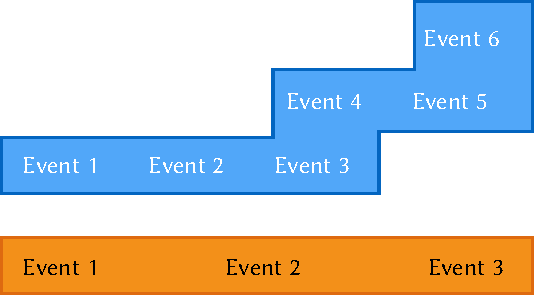
\includegraphics{schema}
	\caption{Visual representation of schema as a colored stripe. Bottom: a simple rectangle connects events that can display in the same row. Top: a rectilinear path connects events that need to locate in different rows.}
	\label{fig:schema}
\end{figure}

Putting it all together, \autoref{fig:sl-overview} shows an example of a complete SchemaLine visualization. The algorithm to produce this is described in \autoref{sec:sl-algorithm}.

\begin{figure}[!htb]
	\centering
	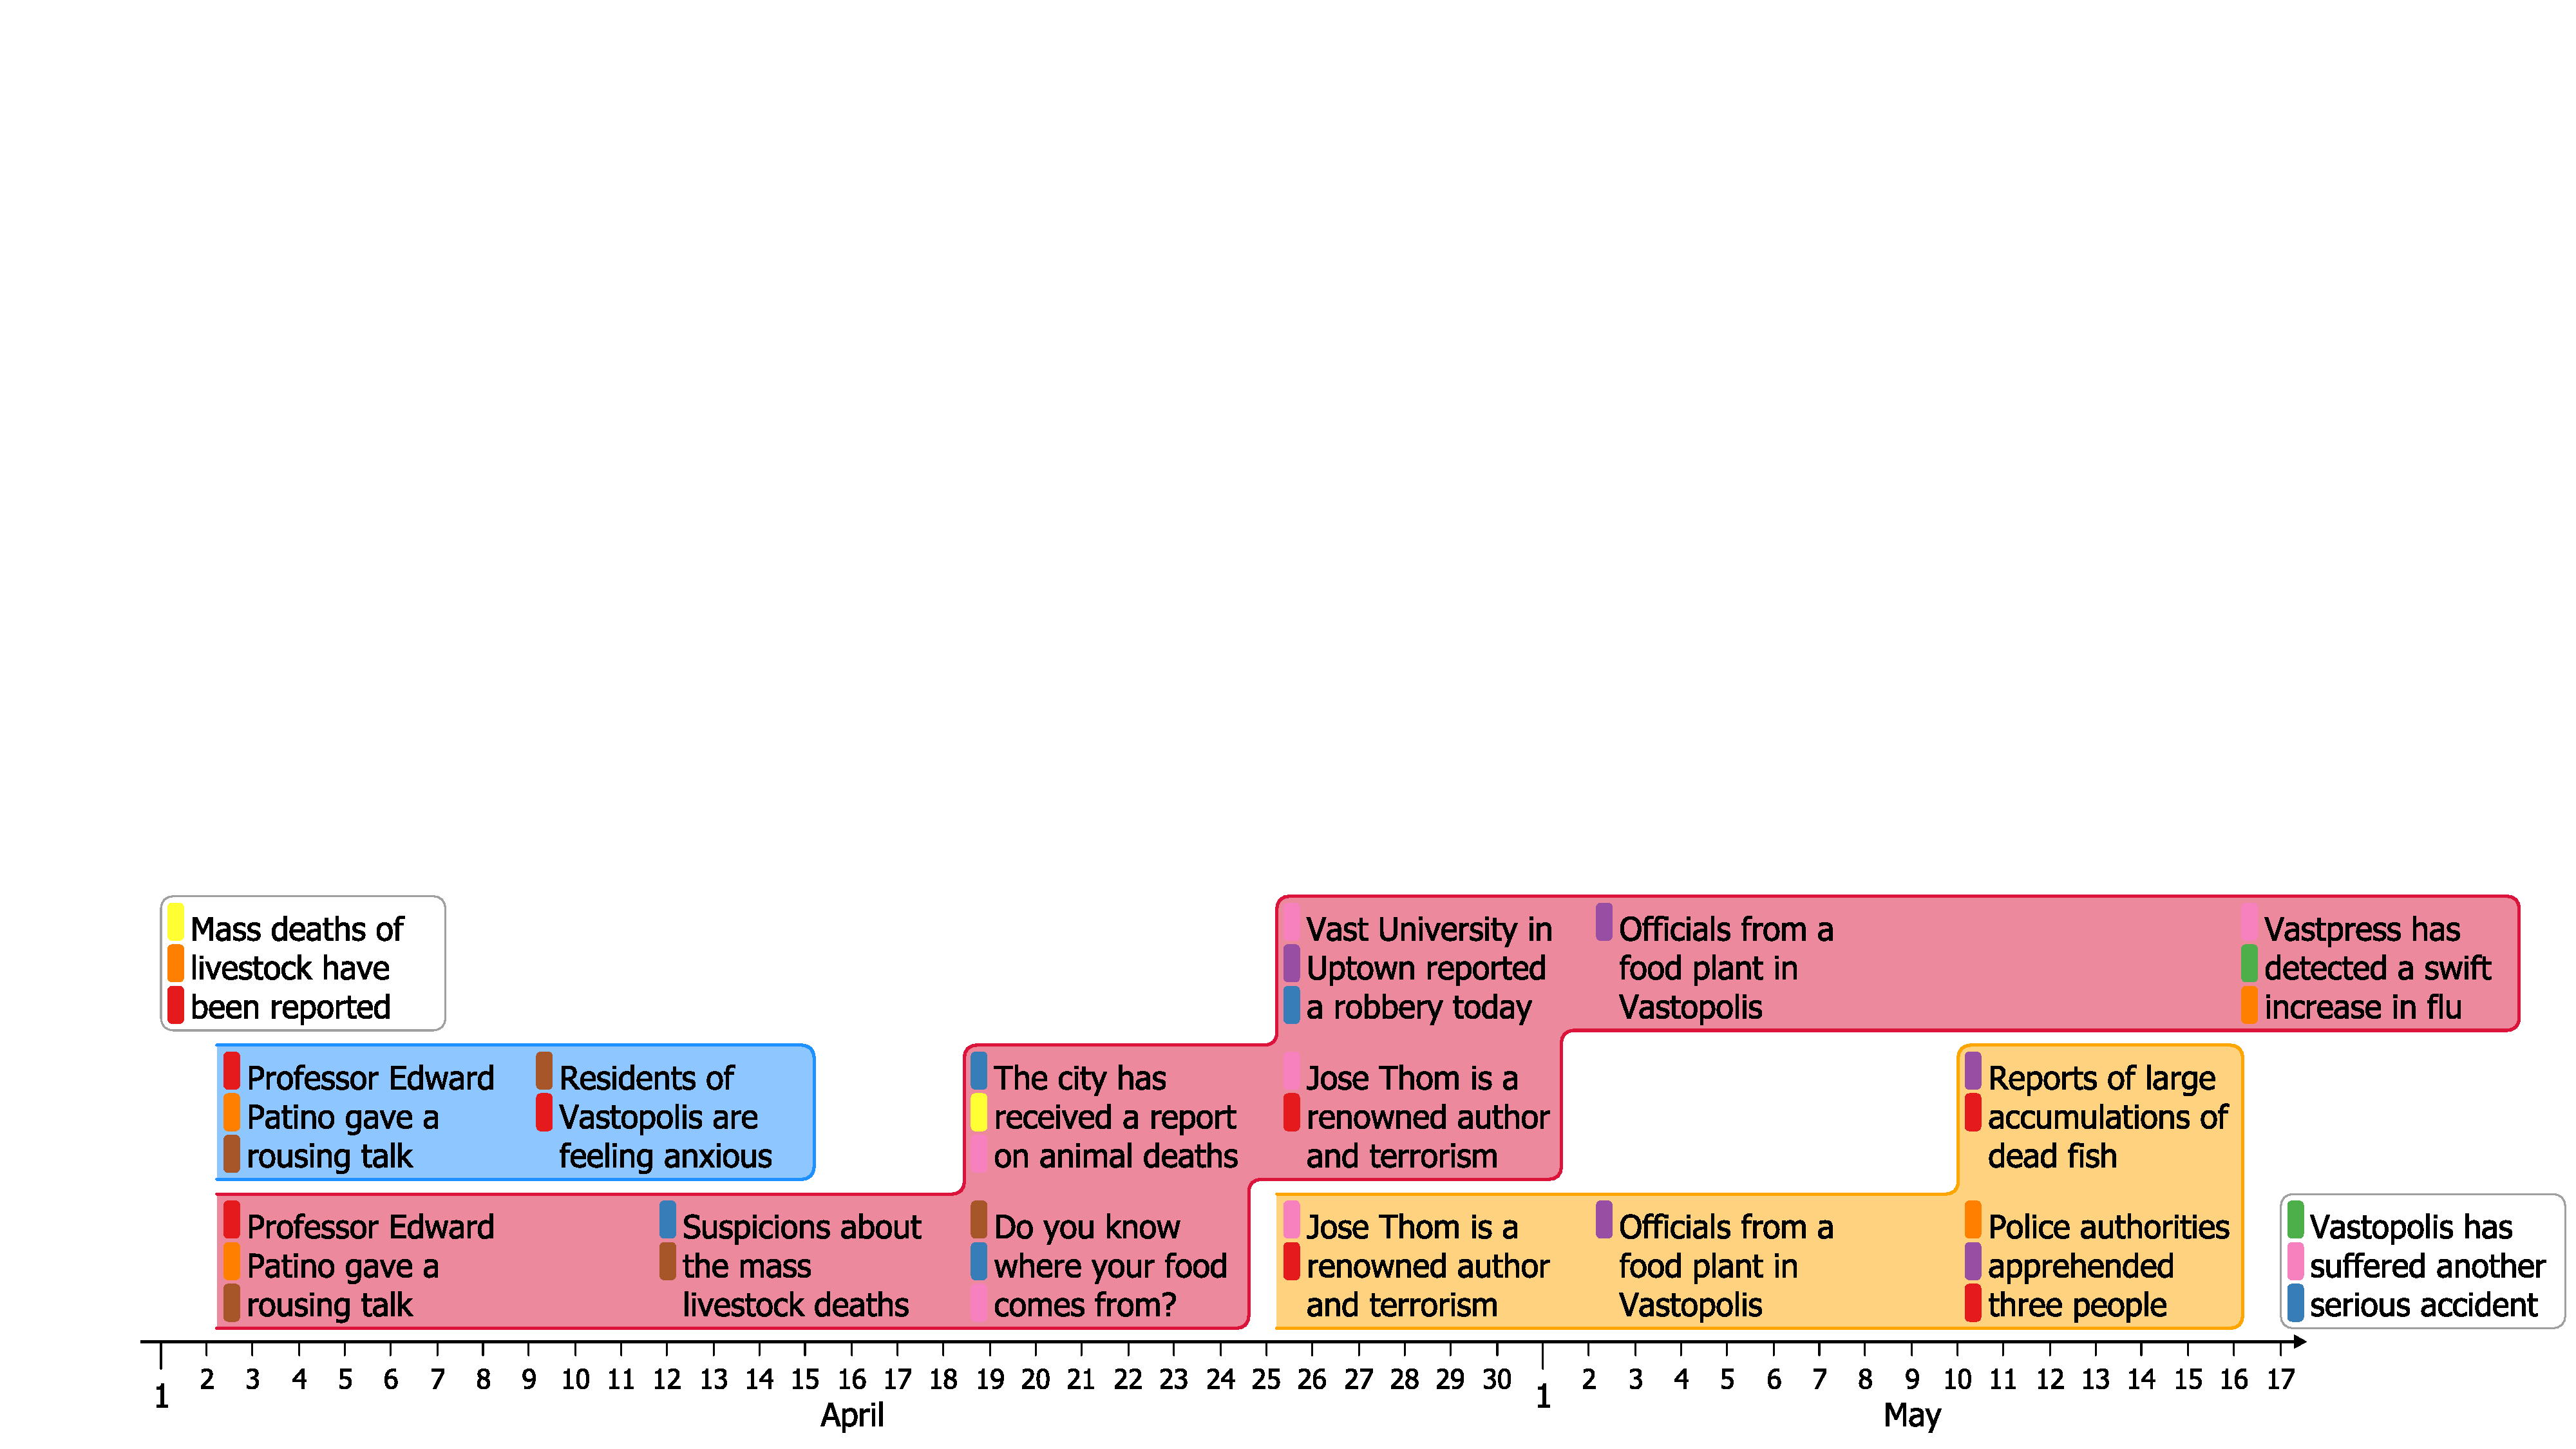
\includegraphics[width=\linewidth]{overview}
	\caption{SchemaLine visualization of annotations. Related ones are connected to form schemas.}
	\label{fig:sl-overview}
\end{figure}

\subsection{Interaction}
To enable analysts to intuitively perform sensemaking activities described in the Data--Frame model (Technical Requirement 3), we follow the design guidelines of fluid interaction proposed by Elmqvist~et~al.~\cite{Elmqvist2011}. More specifically, interactions in SchemaLine 
\begin{itemize}
	\item Produce smooth animated transitions between the state before and the state after an interaction, helping analysts to maintain their mental maps.
	\item Provide immediate visual feedback, enabling analysts to know what is happening and/or what will happen next.
	\item Manipulate directly on the visual representations of events and frames, instead of using extra menus and buttons.
\end{itemize}

During sensemaking, when the analyst recognizes a relationship of events, he or she can group them together and find an account for them (\textbf{connect data and a frame}). This activity is performed by dragging one event and dropping it onto another event, resulting a new frame consisting of these two. While dragging over, a \emph{plus} icon and a rectangle with dashed border surrounding the two events are displayed to indicate that a new frame will be created. 

The analyst can also \textbf{elaborate the frame} by adding more relevant events. This is simply executed by dropping events onto the colored stripe representing the frame. Conversely, to \textbf{preserve the frame}, the analyst can drag its events and drop them onto void space to remove them from the frame. Appropriate informative feedback is displayed in both cases: a \emph{plus} icon for elaboration and a \emph{minus} icon for preservation. \autoref{fig:add-event-frame} shows an example for elaborating the frame.

\begin{figure}[!htb]
	\centering
	\includegraphics{add-event-frame}
	\caption{Elaborating the frame. Dragging and dropping an event onto the blue stripe to add it to that frame. The plus icon indicates the addition behavior if dropping the event.}
	\label{fig:add-event-frame}
\end{figure}

\textbf{Questioning the frame} occurs when the analyst encounters inconsistencies in data. The temporal distribution of events in the frame may suggest some concerns about the plausibility and completeness of the frame. For example, if a frame about one person contains many events in January and March, but none in February; it may be inferred that some data might be missed. To highlight a suspected event, the analyst can double-click on it with the right mouse button. The text of that event will be rendered in red to indicate that it needs more investigation. 

Depending on experience, the analyst can think of multiple explanations for the same set of data. To support \textbf{comparing multiple frames}, we enable the analyst to duplicate events and construct similar frames. By default, dragging an event from one frame and dropping it onto another frame will move it to the new frame. However, holding the \emph{Control} key while dropping an event will instead copy it to the new frame. Also, when two frames are selected, they will be moved vertically next together to facilitate comparison.

The analyst can remove an event from the timeline by dropping it at the bottom of the time axis. A red \emph{remove} icon is displayed as a visual feedback. While searching for a replacement to account for inconsistent and contrary data (\textbf{reframing}), it could be useful to consider discarded data. To enable that, SchemaLine can redisplay events that were removed earlier with half transparency to distinguish them from existing events.

When the analyst thinks that the existing frame cannot account for its data, he or she may  completely discard it and \textbf{seek a new frame}. The frame can be removed by dropping it onto void space. However, its events still remain in the timeline, enabling the analyst to exploit them. Another interaction could be useful is to combine two sets of events together -- we call it ``merge frames''. This can be performed by dragging one schema and dropping it on top of the other schema.
\section{Visual Design}
\label{sec:interface}

\subsection{Event}
An event is represented by a rounded rectangle with a short text inside summarizing its content. All rectangles have the same height to provide a consistent appearance, especially when they are later connected to form a schema (Section \ref{sub:schema-outline}). Rectangles are assigned the same maximum width and long texts are trimmed to fit into their rectangles. The full content of an event will be displayed when it is hovered. Events can include categorical attributes. For example, in news reports, the themes of an article can be sport, fashion or both. Inside the border of an event, small colored rectangles are added to the left of its text to indicate its categories. Only around 12 colors can be distinguished simultaneously in the human view~\cite{Munzner2014}. We choose Set 1 of qualitative colors from ColorBrewer~\cite{Harrower2003} for the colormap. The eight most appeared categories are displayed using these colors and other categories share the same different color. We also plan to combine color with another channel such as texture to increase the number of differentiated categories in the future work. Figure~\ref{fig:event} shows an example of event with three color-coded categories.

\begin{figure}[ht]
\centering
\includegraphics[width=.5\columnwidth]{event}
\caption{An event with three categories. The event is represented as a rounded rectangle with a summarized text inside. On the left side of the text, small color-coded rectangles indicate its categories. The event is positioned along the time axis at when it happens -- 8th of May.}
\label{fig:event}
\end{figure}

An event is left-aligned with its temporal value on the time axis. To reduce cluttering, an event is not visually connected to its corresponding point on the axis. Instead, when the mouse hovers an event, its time point on the time axis is highlighted. The time axis is shown as a horizontal line at the bottom of all events. It consists of two hierarchical temporal scales, which are changed dynamically according to the range of the displayed events. For example, Figure~\ref{fig:event} shows two scales: ``month/day'', but they can switch to ``year/month'' if the range is larger.

\subsection{Schema}
\todo{do the requirements, the design choices should be justified using them}
\todo{don't define schema here. this is all about representation.}
After discovering a number of relevant events or pieces of evidence, the analyst starts combining them to form a \textit{schema}. A schema is a set of related events that are connected to each other in a certain way. For example, a schema might contain all events about a particular person. Figure~\ref{fig:schema} shows examples of schema. 

\begin{figure}[ht]
	\centering
	\includegraphics[width=.6\columnwidth]{schema}
	\caption{.}
	\label{fig:schema}
\end{figure}

\begin{figure}[ht]
\centering
\includegraphics[width=\linewidth]{teaser}
\caption{SchemaLine: each piece of text is an analyst note, positioned along the time axis at when the event happened. Related notes are linked together to form a ``schema'' or ``frame''. There are three frames in this example represented as colored rectilinear paths. Small color-coded rectangles on the left side of notes are ``categories''.}
\label{fig:teaser}
\end{figure}

We consider several design options to connect events within a schema such as using colored/shaped icons or node-link diagrams. However, they all have some drawbacks as discussed in the Related work (Section~\ref{sec:relatedwork}). Computational methods that allow visualize a large number of events with different themes such as ThemeRiver~\cite{Havre2002} do not work either because individual events and interactions are more essential in SchemaLine. \note{I don't quite understand what the `computational' means and the argument follows} Also, it should be easy to follow events within a schema in temporal order. We decided to visualize each schema as a colored stripe, which is inspired by Munroe's hand-drawn visualization~\cite{Munroe2009}. A character line in Munroe's work connects all events happened to that character. Similarly, our schema is a color stripe connecting all events belonging to it. Instead of using a thin line, we use a path with unique width (an event's height) to make enough space to display the event's summary text and allow interaction with individual notes. A rectilinear path is employed to provide a nice visualization rather than direct connection between events. 
\section{Layout and Outline}
\label{sec:sl-algorithm}
This section discusses how to produce the SchemaLine visualization such as the one in \autoref{fig:sl-overview}. The layout of schemas is generated before their outlines are computed based on the layout information.

\subsection{SchemaLine Layout}
Based on the technical requirements, the layout should satisfy these conditions: 
\begin{enumerate}
	\item \textbf{Horizontal position}. Along the time axis, events should be located accurately at when they happen, if possible. This is to meet Technical Requirement 1 -- event representation.
	\item \textbf{Relative order}. However, to address scalability, events can be shifted horizontally as long as their relative order is maintained: $x(e_1) < x(e_2)$ if and only if $e_1$ happens before $e_2$, where $x(e)$ is the horizontal position of event $e$.
	\item \textbf{Overlap free}. Events and schemas are not allowed to intersect each other.
\end{enumerate}

To meet these conditions, we design a layout algorithm consisting of the following four steps (\autoref{fig:sl-layout-overview}):
\begin{enumerate} 
	\item Order the schemas vertically based on their number of events.
	\item For each schema, locate its events satisfying the aforementioned requirements.
	\item Compact the schemas following the order computed in the first step.
	\item Locate the remaining events that do not belong to any schemas. 
\end{enumerate}

\begin{figure}[!htb]
\centering
\includegraphics[width=\linewidth]{layout-overview}
\caption[Summary of SchemaLine layout algorithm]{SchemaLine layout algorithm consisting of four steps. First, the vertical order of schemas is computed. Second, the layout of each schema is generated independently. Third, the schemas are compacted based on the computed order. Last, events that do not belong to any schemas are added to the visualization.}
\label{fig:sl-layout-overview}
\end{figure}

\subsubsection{Order Schemas}
As explained in \autoref{sub:schema}, schemas are vertically stacked to apply the \emph{proximity} principle. This step computes the vertical order of all schemas based on their number of events: the schemas with more events are located under the one with less events. This ordering is based on an assumption that larger schemas (in terms of the number of events) are more relevant than smaller ones, thus are located closer to the time axis. If two schemas consist of the same number of events, the one with longer time range is located under.

\subsubsection{Layout Individual Schemas}
\label{sub:layout-schema}
The second step is to produce the layout for each schema. Events that are members of multiple schemas are replicated, allowing the layout of each schema to be generated independently. Events within a schema are sorted chronologically and added to the timeline in that order. Because all events have the same height, only the row level and horizontal position of each event are needed to computed as follows. 

Initially, an event $e_i$ is located on the same row as the previous one $e_{i-1}$ and at the position proportional to its temporal value (Condition 1 -- horizontal position). If these two events are separate, $e_i$ stays at where it is. Otherwise, two cases will be considered. First, if $e_i$ happens at the same time as $e_{i-1}$, it will be located on the upper row and at the same horizontal coordinate as $e_{i-1}$. Second, $e_{i-1}$ is tentatively shifted to the left to make space for $e_i$, as discussed next. If the shift is unsuccessful, $e_i$ will be located in the upper row as in the first case.

\paragraph*{Shifting Events}
To accommodate more events, the accuracy of the horizontal positions of events can be sacrificed. An event can be shifted horizontally to the left to make space for other events. However, an event should not be shifted too far from its accurate position to avoid misinterpretation from analysts. We set that shifting limit to the width of the event so that the event rectangle still covers its time point on the time axis and provides a reasonable indication of its accurate position. 

During shifting, it is essential to make sure that events do not overlap each other (Condition 3 -- overlap free). Considering an event $e_{i-1}$ is shifted to make space for $e_i$, if it overlaps with another event $e_{i-2}$, then $e_{i-2}$ should be shifted as well. Eventually, all events located on the way of the movement should also be shifted. It is also essential to make sure that the relative order between events is still correct after shifting (Condition 2 -- relative order). Otherwise, events with wrong order need to be shifted as well to reestablish the correct order. Note that if two events happen at the same time, they must be located at the same horizontal position. 

\autoref{fig:layout-schema-example} illustrates the layout algorithm for one simple schema.

\begin{figure}[!htb]
	\centering
	\includegraphics[width=\linewidth]{layout-example}
	\caption[Example of Schema layout algorithm]{Example of Schema layout algorithm. Four events $e_1$, $e_2$, $e_3$ and $e_4$ are added chronologically.}
	\label{fig:layout-schema-example}
\end{figure}

\subsubsection{Compact Schemas}
This third step stacks schemas in the order computed in the first step to produce an overlap-free visualization. However, to make the layout more vertically compact, it is unnecessary to strictly located schemas in that order. Schemas are processed based on the computed order, starting at the bottom row and moving upward. A schema stops when it does not overlap with previously located schemas. In the worst case, it will be located above all other schemas.

\subsubsection{Add Remaining Events}
This last step allocates events that do not belong to any schemas. Events are sorted chronologically and processed in that order. The ideal horizontal coordinate of an event is the position proportional to its temporal value; however, it can also be shifted using the \emph{shifting} method described earlier in \autoref{sub:layout-schema}. An event begins at the bottom row and moves upward until it does not overlap with any other schemas or events after possible shifts. 

\subsection{Schema Outline}
In this section, we describe a process to produce a polygonal outline covering all the event rectangles of a schema. Only horizontal and vertical line segments are used to keep the outline simple yet aesthetic as in \autoref{fig:schema}. The \emph{polygonal path} $P_n$ of a schema that contains $n$ event rectangles $R_1, R_2, ..., R_n$, ordered from left to right, is determined as follows:
\[
P_n=
\begin{cases}
R_1, & n=1 \\
P_{n-1} \oplus R_n, & n > 1
\end{cases},
\]
where $\oplus$ is an operator that appends a rectangle to a polygonal path. As described in the layout of individual schema (Section \ref{sub:layout-schema}), when a new event is added to an existing schema, it has the same row as the previous event (\autoref{fig:outline-right}) or one row higher (\autoref{fig:outline-up}). To produce an aesthetically pleasing path, two other special cases are also considered as described in \autoref{fig:outline-up-one} and \autoref{fig:outline-up-two}. Technically, a path is represented by a list of vertices and is updated when new events are added. \autoref{fig:sl-outline} illustrates how these vertices are updated, added or unchanged for all four those cases.

\begin{figure}[!htb]
	\centering
	\includegraphics{outline-legend}\bigskip\\
	\subcaptionbox{\label{fig:outline-right}$R_3$ is on the right side of the path.}{\includegraphics{outline-right}}
	
	\vspace{.5\baselineskip}
	
	\subcaptionbox{\label{fig:outline-up}$R_3$ is on top of the path.}[.43\linewidth]{\includegraphics{outline-up}}
	\hfill
	\subcaptionbox{\label{fig:outline-up-one}Left of $R_3$ is a bit greater than left of $R_2$.}[.26\linewidth]{\includegraphics{outline-up-smoothing}}
	\hfill
	\subcaptionbox{\label{fig:outline-up-two}Right of $R_3$ is shorter than right of $R_2$.}[.26\linewidth]{\includegraphics{outline-up-shorter}}
	\caption[Rectangle appended into a polygonal path]{Four cases when a new rectangle \colorbox{f2!40}{$R_3$} is appended \textcolor{ForestGreen}{$\pmb{\oplus}$} to a polygonal path -- representing by a dashed polygon. Vertices of the path are colored coded to describe how they are maintained.}
	\label{fig:sl-outline}
\end{figure}

After producing a rectilinear path, all corner bends are made rounded as in \autoref{fig:sl-overview}. The path is filled with the same stroke color but less transparency to make the border stand out with a darker hue. The beginning of the path does not have the border to indicate the flow of events within the path. 
\section{Sensemaking with SchemaLine}
\label{sec:interaction}

%We first discuss about the visual encoding of events and schemata; and then how sense making activities in Data-Frame model are supported in SchemaLine.

%\subsection{Event and Schema Representation}
%\label{sub:visual-encoding}
%\paragraph*{Event Representation}
%%Appearance
%An event is represented by a rounded rectangle with its left side aligned with the event's time on the timeline. To reduce cluttering, events are not constantly connected by lines to their corresponding points on the timeline. Instead, when the mouse is over an event, its time point on the timeline is highlighted. A short text is rendered inside the rectangle to summarize the event. To address the scalability of long texts, we assign a maximum width to event rectangles and trim exceeding texts. The full content will only be displayed when the note is hovered over. All events have a uniform height to give a nice overall appearance, especially when they are connected to form a schema (Section \ref{sub:schema-outline}). Quite often, events are categorical data. For example, in news reports, an article can be classified into sport, fashion or both. SchemaLine adds a small rectangle in each event to color-code its categorization. Eight different colors are supported, which are chosen from qualitative colors -- Set 1 of ColorBrewer \cite{Harrower2003}. All other categories besides eight of the most popular ones will share the same color to address the limitation of small distinguishable colors. We plan to combine colors with other indicators such as texture to increase the number of differentiated keywords in the future work. The number of maximum categories that an event can belong to is configurable to adapt the dataset characteristics. As in Fig.~\ref{fig:notes-only}, maximum four themes of an event can be displayed.
%
%\begin{figure}[ht]
%\centering
%\includegraphics[width=\linewidth]{notes-only}
%\caption{Bigger texts, two events are ok, no need change time. Events are represented by rounded rectangles with uniform height and limited widths for displaying texts. On the left side of the event rectangle, there are some small color-coded rectangles to represent the event's themes.}
%\label{fig:notes-only}
%\end{figure}
%
%%Timeline appearance
%In SchemaLine, the timeline is shown as a horizontal axis at the bottom of the display. Its starting and ending points change dynamically to cover the time span of all events. The timeline consists of two temporal scales. These two scales can also be changed dynamically according to the displayed events. For example, they change from ``month/day'' to ``year/month'' to accommodate large interval increases.
%
%\paragraph*{Schema Representation}
%After discovering a number of relevant events or evidence, the analyst starts combining them to form a \textit{schema}. A schema is a set of related events that are connected to each other in a certain way. For example, a schema can contain all events about a particular person. Multiple schemata can be composed in SchemaLine as shown in Fig.~\ref{fig:teaser}. 
%
%We consider several design options to connect events within a schema such as using colors~\cite{TimeGlider2013} or node-link diagram~\cite{Jensen2003}. However, they all have some drawbacks as discussed in the Related work (Section~\ref{sec:relatedwork}). Computational methods that allow visualize a large number of events with different themes such as ThemeRiver~\cite{Havre2002} do not work either because individual events and interactions are more essential in SchemaLine. Also, it should be easy to follow events within a schema in temporal order. We decided to visualize each schema as a colored stripe, which is inspired by Munroe's hand-drawn visualization~\cite{Munroe2009}. A character line in Munroe's work connects all events happened to that character. Similarly, our schema is a color stripe connecting all events belonging to it. Instead of using a thin line, we use a path with unique width (an event's height) to make enough space for displaying the event's summary text and possible to interact with individual notes. A rectilinear path is employed to provide a nice visualization rather than direct connection between events. An example can be seen in Fig.~\ref{fig:schema} and details of the algorithm to generate the schema layout and outline will be discussed in Section~\ref{sec:layout}.
%\begin{figure}[ht]
%\centering
%\includegraphics[width=\linewidth]{story}
%\caption{A schema with rounded corners.}
%\label{fig:schema}
%\end{figure}

%In the SchemaLine, each white rectangle is an analysis note, linking to the document in the search results that led to this discovery and positioned along the time axis at the point when the event happened. Notes can be grouped together to form a ``story''. There are three stories in this example and they are in red, blue, and orange. In the middle are the results of two searches: ``vastopolis'' and ``terrorist''. At the very top is a list of minimized searches, only showing the keywords. 


%Pirolli and Card~\cite{Pirolli2005} regarded the timeline as an effective tool for the ``Schematize'' task. A timeline can not only reveal the temporal relationships among the findings, but also have a considerable impact on how easily they can be understood. Pennington and Hastie~\cite{Pennington1991} studied the impact of evidence presentation order on juror decision making. They found that information was easier to understand when presented in chronological order and thus had a significant impact on jurors' decisions. 

%\subsection{Sensemaking with Data-Frame Model}
%\label{sub:interactive-editing}
SchemaLine is designed to support all five sensemaking activities in Data-Frame model through fluid user interactions. Following the design guidelines for fluidity proposed by Elmqvist et al.~\cite{Elmqvist2011}, SchemaLine's interactions
\begin{itemize}
	\item use smooth animated transitions between states,
	\item provide immediate visual feedback on interaction, and
	\item use direct manipulation of visual representations.
\end{itemize}

Sensemaking activities in Data-Frame model involve two different types of entities: \textit{data} and \textit{frame}. We allow direct manipulation of visual representations of data and frame, instead of invoking menus and buttons to perform actions. The first sensemaking activity in the Data-Frame model is to \textbf{construct a new frame} by connecting relevant data. It can be performed in SchemaLine by \textit{dragging one event and dropping it onto another event}. A \textit{plus} icon and a \textit{dashed rectangle} surrounding the two events are displayed to indicate that a new frame will be created. When dropping the event, a color stripe representing a frame will be formed by connecting these two events, and a smooth animated transition is used to improve user perception.

Besides dropping an event on top of another event, the user can drop it onto the color stripe to add that event to an existing frame (\textbf{elaborate a frame}). Conversely, the user can drag an event belonging to a frame and drop it onto the void space to remove it from the frame (\textbf{preserving a frame}). Appropriate informative feedback is displayed, \textit{plus} icon for addition and \textit{minus} icon for subtraction, and a smooth animated transition is used to improve user perception. Fig.~\ref{fig:drag-drop-note} shows an example of adding an event into a frame.
\begin{figure}[ht]
\centering
\includegraphics[width=\linewidth]{add-event-frame}
\caption{Each frame is represented as a colored stripe. Dropping an event onto the blue stripe means adding that event into the blue frame to elaborate it.}
\label{fig:drag-drop-note}
\end{figure}

\textbf{Questioning a frame} occurs when the user encounters inconsistencies in data within a frame. The temporal distribution of events in the frame may suggest some concerns about the validity or completeness of the frame. For example, if a frame about one person contains many events in January and March, but no events are found in February, then it may be inferred that there could be some data missing. The analyst can mark a suspected event by right-mouse double-clicking on it. Red color text is used to indicate that the event needs more investigation. 

Dragging an event from one frame to another frame will remove it from the old frame and add it to the new frame. However, holding \textit{Control} key when dropping will instead copy the event to the new frame. This interaction allows the analyst to duplicate events to create several similar frames and compare them (\textbf{comparing frames}). When two frames are selected, they will be moved closer together to allow easy comparison, irrespective of the frames ordering generated by the layout algorithm. The user can drag an entire frame and drop it onto another frame to merge all events together. The user can also drop the frame onto the void space to take apart the frame and release its events. This interaction is useful when the user thinks that the frame is completely wrong and wants to construct a new frame (\textbf{reframing}).

Other interactions with events are also designed to be intuitive. Left-mouse double-clicking on an event opens its full content. Dragging an event with the right mouse button can change the event's date. This feature is useful because the report date is not always the date when the event actually occurred; for example, ``yesterday there was a bomb attack in ABC''. Dragging an event outside the boundary of the timeline will remove it from the system (with \textit{remove} icon as informative feedback).

Once any change is made on SchemaLine, such as moving an event from one frame to another, an animation is shown of smooth transition between the changes to help analyst update their ``mental map''. To achieve this, the layout algorithm (Section \ref{sub:schema-layout}) computes the new event rectangle locations. Then, the outline algorithm (Section \ref{sub:schema-outline}) runs at every step of the interpolation between the old and the new locations to produce intermediate polygon paths based on the updated event locations.
\section{Evaluation}
\label{sub:sl-evaluation}
SchemaLine was integrated into an existing visual analytics system to evaluate its usefulness in making sense of temporal relationship in intelligence analysis. The integration will be discussed next and followed by a sensemaking case study.

\subsection{Application}
% Overview of INVISQUE
We integrate SchemaLine into INVISQUE~\cite{Wong2011} -- a visual analytics system designed for interactive exploration of text documents. INVISQUE provides full-text search and organizes the search results into a two-dimensional canvas, with each dimension representing a configurable attribute. For example, it may be useful to order academic articles horizontally by publication date and vertically by citation count. Search results are shown as a cluster of \emph{index-cards}, each representing a document with selected information such as publication title, date, keywords and authors. \autoref{fig:invisque} shows a screenshot of INVISQUE.

\begin{figure}[!htb]
	\centering
	\includegraphics[width=\linewidth]{invisque}
	\caption{INVISQUE interface. It shows two clusters of search results for ``network'' and ``security'' from a publication dataset. Each index-card in a cluster represents an article with meta information displayed on it.}
	\label{fig:invisque}
\end{figure}

% Integration
We add an \emph{annotation} feature to allow analysts to record their thoughts while reading documents. Technically, the association between an annotation and its containing document should be saved for potential provenance retrieval. These annotations are important to analysts, thus are also displayed on the index-cards together with other meta information. The annotations are used  as the input \emph{events} of the SchemaLine visualization. SchemaLine is placed at the bottom of INVISQUE. After the analyst makes a note, or annotation, it is immediately added to SchemaLine as a new event. Double clicking on an event will open the document containing that note as an index-card, enabling the analyst to quickly reexamine the original information source.

% Attribute mapping
The \emph{temporal information} of documents, such as ``publication date'', is initially assigned to that of events, and can be corrected later by analysts. This feature can be useful because the report date is not necessary the same as the date when the event actually occurred. For example, a news article published today can be written about a bomb attack that happened several days ago. The analyst can make the correction by dragging an event with the right mouse button along the time axis and dropping it at the desired date. 

The \emph{label} of an event simply maps to the content of an annotation itself. In INVISQUE, we color code search keywords that contain annotated documents, and use them as \emph{categories} for events. Because a document can be returned from different searches, it can thus contain multiple categories. This mapping provides context for the annotations: what did I search for (the original keyword) and what are other related concepts (other search keywords returning the same document)? This context may help analysts discover interesting patterns through their annotations. \autoref{fig:invisque-schemaline} shows a screenshot of INVISQUE with SchemaLine integrated.

\begin{figure}[!htb]
	\centering
	\includegraphics[width=\linewidth]{invisque-schemaline}
	\caption{INVISQUE with SchemaLine at the bottom. The timeline consists of three events, which are notes taken by an analyst. Color coded categories of events indicate keywords that were searched for.}
	\label{fig:invisque-schemaline}
\end{figure}

\subsection{Case Study}

\subsubsection{Design}

\paragraph{Method}
Evaluating the usefulness of SchemaLine in supporting sensemaking can be categorized as \emph{evaluating visual data analysis and reasoning} -- one of the seven scenarios in evaluating information visualization proposed by Lam~et~al.~\cite{Lam2012}. The goal of this evaluation scenario is to explore whether and how a visualization tool supports participants to make sense of the given tasks and generate relevant knowledge. During solving sensemaking tasks, participants may employ various strategies. Their processes and outcomes are also highly context-sensitive, making it difficult to quantify and compare their performance. Therefore, sensemaking evaluations are typically case studies with real-world tasks performed by domain experts. We conducted a case study to explore how SchemaLine supports analysts to solve an intelligence analysis task, focusing on how it enables them to perform sensemaking activities in the Data--Frame model. However, due to a limited access to these resources, we instead use a realistic investigative task with graduate students.

\paragraph{Task}
We used the task from Mini Challenge 3 of the IEEE VAST Challenge 2011~\footnote{\url{http://hcil2.cs.umd.edu/newvarepository/VAST Challenge 2011/challenges/MC3 - Investigation into Terrorist Activity/}}, which requires the participants to identify any imminent threats from the given dataset. We chose this task because it resembles a real intelligence task, demanding analysts to read many documents, extract relevant pieces of evidence and assemble them in order to derive insight and find a reasonable answer to the given question. Also, the solution was provided and well-tested by the community, making it possible to assess participants' performance. The participants were given INVISQUE with SchemaLine integrated to solve the task. 

\paragraph{Dataset}
The original dataset contains more than four thousand news reports, 36 of which are relevant to criminal activities and are manually added by the Challenge committee. Both participants in our pilot test failed to find any imminent threats after one and a half hours. Most of their time was spent on reading long (more than 500 words) but irrelevant documents. The reason could be that INVISQUE does not support text-mining features such as entity extraction, which is crucial in analyzing a large document collection. However, the goal of this evaluation was to assess how SchemaLine can provide additional sensemaking support to INVISQUE rather than assessing INVISQUE itself. Therefore, in the main study, we removed all irrelevant documents that are not part of the ground truth to make the dataset size more manageable. The new dataset only contains the 36 relevant documents, 29 of which are correct answers including five criminal activities: food poisoning (13 documents), hacking (3), dirty bomb (6), arms trafficking (4), and money laundering (3). Other documents are isolated cases, acted as false leads. We expected that participants could complete the task within a reasonable amount of time, without affecting the goal of the study. 

\paragraph{Participants and Procedure}
We were unable to recruit real intelligence analysts for the study. Instead, we recruited three graduate students with different backgrounds:  one in visual analytics (surrogate for visualization expert -- \textbf{P1}), one in law (surrogate for domain expert -- \textbf{P2}), and one in computer network (neutral background -- \textbf{P3}). After being introduced features of INVISQUE and SchemaLine, participants had a chance to practice with a trial sensemaking task for 15 minutes. The main task was followed and lasted for one hour. The participants were asked to report the criminal activities they had discovered with supporting evidence. Semi-structured interviews were followed to gain deeper understanding of the sensemaking processes.

\subsubsection{Results and Discussion}
We first summarize the three sessions and present our collective findings next.

\paragraph{Participant 1}
\textbf{P1} began searching for ``bomb'', examined the search results, and searched for  a refined keyword ``dirty bomb''. He took notes in three documents and then linked these notes together (\emph{connect data and a frame}). He then searched for ``Network of Dread'', which was mentioned in one of documents related to the dirty bomb attack. He took a note in the new returned document and dropped it onto the ``dirty bomb'' schema (\emph{elaborate the frame}). While investigating, he encountered an article about a man carrying a frozen turkey having wires coming out of it, which was suspected as a bomb. At first, he dropped the ``turkey bomb'' note onto the ``dirty bomb'' schema. Then, he wondered whether it was a real bomb. After thinking for a while, he removed it out of the schema (\emph{preserve the frame}). \textbf{P1} found the ``dirty bomb'' attack with 4/6 correct pieces of evidence. \textbf{P1} took many notes in documents related to the ``food poisoning'' case; however, he could not link them together because he said that ``I'm not familiar with bio-attack so I couldn't think of it as a threat''. 

\paragraph{Participant 2}
\textbf{P2} took an overview step before searching. He quickly looked at all 36 document titles to have a glimpse of the dataset as well as to detect potential search keywords. Then he searched for ``animal deaths'', read the results, took notes and grouped them together (\emph{connect data and a frame}). He was satisfied with the evidence he found for that crime and switched to read another interesting article ``Library Computer Left'' he came across. From that, he searched for several related terms such as ``computer'' and ``hackers''. He figured out that a group called ``F-alliance'' stole computers from the library and attempted to hack a bank. He dropped a ``computer stolen'' note on top of a ``bank hacking'' note to form a new explanation for the case (\emph{connect data and a frame}). He found another article related to hacking but he said ``I won't drop it to this group because it's just an announcement from the government about potential threats'' (\emph{preserve the frame}). During further investigation, he created another group of notes related to ``bioterrorism'' and ``Prof. Patino''. Then, when figuring out that the reason of the mass deaths is a spore-forming microbe, which is also mentioned in Prof. Patino's talk, he dropped that new group onto the ``animal deaths'' group to combine all notes together because he thought that they were related (\emph{merge frames}). Observing the order of events in the new group on the timeline, he said ``The equipment of Patino was stolen after the animal deaths report, so they couldn't be used in that case. This is the group of a potential threat in using bioterrorism.'' (\emph{elaborate the frame}). \textbf{P2} found the ``hacking'' case with 2/3 correct pieces of evidence and the ``food poisoning'' case with 9/13 correct pieces of evidence. \autoref{fig:evaluation} shows the computer screen of \textbf{P2} when he reported his findings.

\begin{figure*}[!htb]
	\centering
	\includegraphics[width=\linewidth]{evaluation}
	\caption{Final screen of participant \textbf{P2}. Top: a trail of his keyword searches, collapsed after being read. Middle: search results in index-card metaphor. Bottom: two schemas containing notes as supporting evidence of criminal activities he found.}
	\label{fig:evaluation}
\end{figure*}

\paragraph{Participant 3}
\textbf{P3} searched for a few keywords related to criminal activities before examining the search results such as ``bomb'', ``terrorism'', ``money'' and ``hack''. He took and group notes about ``money laundering'' together (\emph{connect data and a frame}). Then, he read articles from ``terrorism'' search results. He followed the article content to search for relevant information such as ``Paramurderers of Chaos'' -- a terrorist group. During further investigation, similar to \textbf{P2}, he also combined two groups of notes -- ``Paramurderers of Chaos'' and ``food supply'' -- together when discovering evidence linking the two groups (\emph{merge frames}). When presenting his findings, he shared that SchemaLine prompted him to look for missing information. ``I noticed the gap between these two events [pointing to the timeline]; then I knew I probably missed something there'' (\emph{question the frame}). \textbf{P3} found the ``food poisoning'' case with 6/13 correct pieces of evidence, and a perfect 3/3 pieces of evidence in the ``money laundering'' case. 

\paragraph{Discussion}
% All take notes, build schemas
Three participants applied different sensemaking strategies. \textbf{P1} started with a potential search keyword for criminal activities and kept following the search results. \textbf{P2} initially scanned the titles of all documents to have an overview of the dataset. \textbf{P3} planned ahead what he wanted to search for and sequentially executed it. However, all of them extensively took notes and constructed explanatory frames from them. These frames presented various forms: a concept (bioterrorism), a criminal activity (dirty bomb), a person (Prof. Patino) and a group of people (Paramurderers of Chaos). All participants also employed a variety of sensemaking activities described in the Data--Frame model, supported through fluid interaction in SchemaLine: connect data and a frame, elaborate the frame, question the frame preserve the frame and merge frames.

% temporal sensemaking
All participants appreciated the automatic addition of analyst notes to SchemaLine. \textbf{P1} thought that he would have a problem if the system did not support that: ``I can remember what happened but it was difficult to remember when they happened''. They found that the chronological order of events provides cues to them to construct the story lines. \textbf{P2} shared that he read the news about the robbery at Vastopolis university and the Prof. Patino's talk about bioterrorism. However, he did not have any insight at that time. When looking at his two notes on the timeline, he thought that the extremely expensive equipment in Prof. Patino's lab could be the reason of the robbery. 

% intuitive interface & presentation
All participants commented that the interaction between data and frame was very intuitive. \textbf{P1} said ``I think I don't even need training and still can figure out how it works''. \textbf{P3} appreciated the transition effect when adding or removing notes because ``it helped me to understand what is going on''. All participants were confident while presenting their analyses. \textbf{P3} even opened the original document (double-clicking on the note) several times to highlight the relevant text. He said that the connection between the note and the containing document enabled him to quickly find the information source when needed.
\section{Conclusion and Future Work}
\label{sec:conclusion}

In this paper, we introduced a new timeline visualization, SchemaLine, which is designed to support sensemaking. More specifically, it facilitates the schematization process in the Pirolli-Card model and targets all sensemaking activities in the Data-Frame model. The SchemaLine layout algorithm produces simple, compact, but aesthetically pleasing timeline visualizations. It replaces menu and buttons with fluid user interactions to perform all necessary tasks, and can be integrated within larger visual analytic systems. Our preliminary evaluation suggests that the design of SchemaLine is supportive of sensemaking tasks. It was clearly a helpful aid to users in analysis of the scenario, as evidenced by their usage patterns and feedback. 

As future work, a more formal evaluation would be beneficial -- perhaps even following integration of SchemaLine into a number of different systems, to allow the specific effect to be separated from the rest of the system. In terms of design of the SchemaLine itself, there are a number of improvements that could be added. Shared events between frames could be better visualized (at present, the event is simply duplicated). There are also obvious issues with scalability: while the timeline will scale comparatively well with number of events, it will scale badly with number of frames, since the set of effective qualitative colors is quite small. Other cues such as texture or line style may help with this problem, but to discover this will require further experimentation.
%\chapter{TimeSets}

\graphicspath{{Chapter4/figures/}}

In this paper, we introduce a novel timeline visualization technique, TimeSets, that helps make sense of complex temporal datasets by showing the set relationships among individual events. TimeSets visually groups events that share a topic, such as a place or a person, while preserving their temporal order. It dynamically adjusts the level of detail for each event to suit the amount of information and display estate. Various design options were explored to address issues such as one event belonging to multiple topics. A controlled experiment was conducted to evaluate its effectiveness by comparing it to the KelpFusion method. The results showed significant advantage in accuracy and user preference.

\section{Introduction}
In the previous chapter, SchemaLine is shown to be effective in exploring temporal relationship of intelligence sensemaking by allowing analysts to construct narratives (or schemas) from their annotations (or events). However, it does not allow an event to be part of multiple schemas, which is common in early data exploration. Also, literature in sensemaking theory (\autoref{sub:lr-sensemaking})  suggests the same requirement. Pirolli and Card's model shows that analysts can generate multiple hypotheses from the same information they found. Data--Frame model proposes that multiple frames can be created to account for the same data. Therefore, it is critical for a timeline visualization for sensemaking to effectively show both \emph{temporal} and \emph{set} (for generality) information of events simultaneously.

Back in 1765, one of the oldest documented timelines produced by Joseph Priestley -- the Chart of Biography~\cite{Priestley1765} -- already denotes sets of elements. The timeline includes two thousand famous persons from 1200 BC to 1800 AD classified into six categories based on their most well-known achievement. The timeline is divided into six horizontal bands, one for each category, to visualize the set relations. However, it is clear that an element cannot be part of multiple sets. 

More sophisticated techniques have been designed to visualize multiple-set events. One technique is to assign set membership to a visual channel of element icons such as color hue or shape~\cite{TimeGlider2016}. However, events in the same set are not necessarily located close to each other, making it difficult to follow them chronologically or to have an overview of the distribution of events~\cite{SimileTimeline2009,TimeGlider2016}. Another common approach is to visually connect events in the same set~\cite{Kumar1998}. Such a method can introduce extra edges and crossings, which hamper the readability of the timeline. 

There has been considerable work on set visualization, which commonly uses closed contours as in Venn or Euler diagrams. Texture and color can be used to depict more complex set relations~\cite{Ware2013}. However, these cannot be applied in timelines because the horizontal positions of events are fixed. Techniques that visualize set relations of data items with fixed locations could be good alternatives. To connect same-set elements, Bubble Sets~\cite{Collins2009a} draws an iso-contour surrounding them, LineSets~\cite{Alper2011} uses a B\'{e}zier curve passing through all the elements, and KelpFusion~\cite{Meulemans2013} employs both lines and areas to connect elements. However, simply applying these methods on top of existing timelines could introduce many crossings between text and visual elements of sets that may reduce readability.

Similar to SchemaLine, this chapter also focuses on making sense of temporal relationship in intelligence analysis domain. However, it addresses more complex relationship by effectively displaying both temporal and set information in data. More specifically, we design a novel timeline visualization -- TimeSets -- to

\begin{itemize}
	\item Clearly shows the events within a set over time and their relationships with other sets.
	\item Dynamically adjusts the level of details of each event to suit the amount of information and display estate.
	\item Uses color gradient backgrounds for events belonging to multiple sets and curved set outlines to emphasize its grouping.
\end{itemize}

To show possible applications of TimeSets, we discuss two case studies with intelligence analysis and publication data exploration. Also, a controlled experiment was conducted to evaluate the effectiveness of TimeSets. The results showed that TimeSets was significantly more accurate than KelpFusion~\cite{Meulemans2013} -- a state-of-the-art set visualization method, and was the preferred choice by the participants for aesthetics.
%\section{Related Work on Visualizing Time and Sets}
\label{sub:ts-review}

This section discusses related work on visualizing set relations in timelines and techniques for visualizing general sets.

\subsection{Set Relations in Timelines}
As presented in the Literature Review chapter, \autoref{sub:lr-design}, Gestalt principles are often used to represent set relations among elements. This section discusses the application of those principles in visualizing set relations of events in timelines.

The principle of \textit{similarity} states that objects are perceptually grouped together if they are similar to each other. This principle is extensively applied to show set relations in timelines by using colors and shapes. Time indicators as icons for time-point events and bars for interval events are colored according to event set memberships~\cite{SimileTimeline2009,Wang2008}. Different shapes for icons~\cite{TimeGlider2016} and bars~\cite{Plaisant1998} are also used to distinguish set memberships. It is more challenging to represent multiple set memberships. LineSets~\cite{Alper2011} uses concentric circles for icons, where each circle is colored to represent one set.

According to the \textit{proximity} principle, objects that are close together are perceived more related than objects that are located further apart. In the Chart of Biography~\cite{Priestley1765}, people within a category are placed in a horizontal band, away from people in other categories. LifeLines~\cite{Plaisant1998} splits medical records into different sets, such as \textit{medication} or \textit{diagnosis}, and places them into vertically stacks, which works well if no two sets overlap. Storyline visualizations~\cite{Tanahashi2012,Liu2013} use curved lines to show interactions among characters within the movie timeline. Character lines converge to a bundle if they appear in the same interaction, and diverge when the interaction ends. Each line can be considered as a set passing through all of its members, and each interaction is a multi-set event. Thus, this method only works for interval events.

Elements tend to be grouped together if they are visually connected. Following this \textit{uniform connectedness} principle, tmViewer~\cite{Kumar1998} links related entities with line segments. Different line colors, thicknesses, and styles were used to distinguish set relations. This method can show events with multiple set memberships by connecting them with multiple edges. However, extra edges and crossings may negatively impact the readability of the timeline.

When similarity and proximity are applied together, the later principle dominates~\cite{Ware2013}. Moreover, uniform connectedness is stronger than proximity~\cite{Palmer1994}. For example, objects with different colors and shapes but are located close together are more likely to be perceived as a group, and distant objects but with a closed contour surrounding them also provide a strong sense of grouping. Applying these ideas to visualize set relations for timelines, methods relying on similarity such as colored icons~\cite{Wang2008} are less effective than spatial grouping methods such as LifeLines~\cite{Plaisant1996}. And those, in turn, are less effective than methods using line segments such as tmViewer~\cite{Kumar1998}. 

\subsection{Set Visualizations}
Sets and their relationships can be visualized using Venn~\cite{Ruskey1997} or Euler~\cite{Rodgers2014} diagrams. Simonetto~et~al.~\cite{Simonetto2009} propose a technique to visualize sets that were previously not possible with Euler diagrams. However, the complex shapes it produces may reduce visualization readability. A controlled study by Henry-Riche and Dwyer~\cite{Riche2010} shows that for complex set intersections, duplications of shared elements result in a better performance in readability tasks than a none-duplicated visualization with more complex shapes. A state-of-the-art report by Alsallakh~et~al.~\cite{Alsallakh2014} provides a comprehensive survey of set visualization techniques. In this section, we discuss a few techniques that can be applied atop elements with fixed positions so that they can be used to visualize set relations for timelines. 

Techniques without such constraints include Bubble Sets~\cite{Collins2009a}, LineSets~\cite{Alper2011}, and KelpFusion~\cite{Meulemans2013}. These methods employ the connectedness principle of the Gestalt laws~\cite{Palmer1994} by connecting set elements using extra visual elements. Bubble Sets draws an iso-contour surrounding elements within a set. This iso-contour is filled with a semi-transparent color so that the intersection between sets is shown as an area of blended color. Collins~et~al.~\cite{Collins2009a} provide an example of applying Bubble Sets to a timeline, with a force-directed algorithm used to adjust the vertical positions of elements while the horizontal positions along the time axis are fixed. 

LineSets applies a B\'{e}zier curve to connect data items. The curve follows the shortest path passing through all elements in the set. Its study shows that LineSets outperforms Bubble Sets in certain readability tasks~\cite{Alper2011}. KelpFusion, a hybrid technique, uses lines for data-sparse areas and surfaces for data-dense areas. The results of an evaluation on readability tasks~\cite{Meulemans2013} demonstrate that it outperforms Bubble Sets in both accuracy and completion time, and outperforms LineSets in completion time. There has been no reported attempt to apply LineSets or KelpFusion to timeline visualizations. It is expected that crossings between lines or areas and the event text may reduce the readability of timelines.
\section{Visual Design}

\subsection{Event}
An event is represented as a line of text -- \emph{label} -- summarizing its content, and a glyph indicating its temporal information. For a time-point event, a \emph{circle} is shown at the left of the label. For an interval event, a \emph{bar} is shown at the top of the label. When two interval events overlap, their time bars are displayed with half opacity to make the intersection visible. To accommodate a large number of events, labels have three possible levels of detail: 
\begin{enumerate}
	\item \textbf{Complete}. The entire label is shown.
	\item \textbf{Trimmed}. Only the first few words are shown and ended with three dots (\dots) to indicate that the visible label is incomplete.
	\item \textbf{Aggregated}. Events are grouped and labeled with the total number of them. A colored border is added to the label to make the aggregate more noticeable. The time bar of an aggregate spans the starting time of its earliest event and the finishing time of its latest event.
\end{enumerate}	

Figure~\ref{fig:event-representation} shows examples these different visual representation of events.

\begin{figure}[!htb]
\centering
\includegraphics[width=.8\columnwidth]{figure2}\caption{Visual representations of events. Top row, left to right: a complete time-point event, a trimmed time-point event, and a aggregate of 10 events. Bottom row, left to right: an interval event, and two overlapping interval events.}
\label{fig:event-representation}
\end{figure}

\subsection{Set}
\subsubsection{Design Overview}
As discussed in Section\note{ref}, Gestalt's principles of grouping are commonly used to show set relationships among events, most effectively are \emph{proximity} and \emph{uniform connectedness}. Therefore, we also apply these two principles in our design: events belonging to the same set are located close together, and the background of an entire set is colored to make its events visually connected.

Spatial grouping is achieved through vertical positioning because the horizontal position of each event is already fixed by its temporal information. Sets are stacked vertically, and each set is further divided into a maximum of three \emph{layers}: the top and the bottom layer for events shared with the set above and below respectively (if they exist), and the middle layer for other events in the set. Figure~\ref{fig:layering} shows an example of a layering for three sets.

\begin{figure}[!htb]
\centering
\includegraphics[width=.5\columnwidth]{figure3}
\caption{Layering for three sets $S_1$, $S_2$, and $S_3$. $L_2$ includes events shared by $S_1$ and $S_2$, and $L_4$ includes events shared by $S_2$ and $S_3$. Shared events are shown in red. $S_2$ consists of events in three layers $L_2$, $L_3$, and $L_4$.}
\label{fig:layering}
\end{figure}

Shared events between two non-neighboring sets can reside in one set and connect to the other set using visual links such as curves~\cite{Alper2011} or areas~\cite{Meulemans2013}. Figure~\ref{fig:layering-1} shows an approach to connect shared events (red squares) using straight edges and link them to the orange set to indicate that they also belong to that set. An alternative approach is to duplicate shared events in both sets. In Figure~\ref{fig:layering-2}, red squares are duplicated in both the green and orange sets. Duplication consumes more display space and could make viewers confuse when seeing same events multiple times. However, it ensures all events of the same set being located close together, which makes the visualization compact. Also, a study by Henry Riche and Dwyer~\cite{Riche2010} shows that complex set-intersection shapes reduce readability compared to item duplication. Aiming for a clear visualization, which is crucial for interactive set construction, we decide to duplicate events that belong to non-neighboring sets. Confused duplication and scalability will be addressed later using interaction and layout algorithm respectively.

\begin{figure}[!htb]
	\centering
	\subcaptionbox{Shared events are connected by edges in the green set, and linked to the orange set.\label{fig:layering-1}}[.47\columnwidth]
	{\includegraphics[width=.35\columnwidth]{figure4a}}
	\hfill	
	\subcaptionbox{Shared events are duplicated in both green and orange sets.\label{fig:layering-2}}[.47\columnwidth]
	{\includegraphics[width=.35\columnwidth]{figure4b}}
	\caption{Shared events (red squares) visualization of two non-neighboring sets.}
	\label{fig:layering-compare}
\end{figure}

In subsequent sections, we discuss the detail of the set visualization algorithm, which consists of two main steps: generating set shapes, and then coloring them.

\subsubsection{Shape Generation}
\label{sub:shapesgeneration}
This algorithm takes as input a list of bounding-boxes of the set's events, and generates a closed-curve containing all these boxes. The sizes and positions of the bounding boxes are decided by the layout algorithm described in the next section. A rectilinear shape can be generated using a scan-line algorithm~\cite{Foley1997}, as shown in Figure~\ref{fig:shape1}. The number of bends along the border is often used to assess the aesthetics and legibility of visualizations~\cite{Tanahashi2012}. Even though the generated shape provides the minimal \textit{data-ink} ratio~\cite{Tufte1986}, a large number of line bends may reduce its legibility. 

\begin{figure}[!htb]
	\centering
	\subcaptionbox{The original rectilinear shape generated by a scan-line algorithm.\label{fig:shape1}} 
	{\includegraphics[width=.47\columnwidth]{figure5a}}
	\hfill
	\subcaptionbox{The simplified shape by flattening and removing jags (red eclipse).\label{fig:shape2}}
	{\includegraphics[width=.47\columnwidth]{figure5b}}
	\caption{Rectilinear shape generation.}
	\label{fig:shape}
\end{figure}

To reduce the number of line bends, the top and the bottom sides of the set outline are flattened. The left and right sides  are kept unchanged because they indicate the temporal information of events. On both sides, the outline can be ``jagged'' if two events start or end close to each other. Those close vertical segments are combined to reduce line bends if their horizontal gap is smaller than some threshold. This trades off time accuracy for outline smoothness and can be adjusted by the user. Figure~\ref{fig:shape2} shows the result of this simplification. 

To reduce the degree of line bends, vertical segments are converted to diagonal ones wherever possible, such as  $e_2$ and $e_3$ in Figure~\ref{fig:generation1}. Smoother lines are easier for users to follow~\cite{Kim2010}, thus diagonal segments are further converted to B\'{e}zier curves, and squared corners are replaced by quadrant arcs as in Figure~\ref{fig:generation2}.

\begin{figure}[ht]
	\centering
	\subcaptionbox{Vertical segments $e_2$ and $e_3$ are converted to diagonal ones (dashed lines).\label{fig:generation1}}
		{\includegraphics[width=.47\columnwidth]{figure6a}}
	\hfill
	\subcaptionbox{Squared corners are replaced by quadrant arcs. $e_2$ and $e_3$ are smoothened by B\'{e}zier curves.\label{fig:generation2}}
		{\includegraphics[width=.47\columnwidth]{figure6b}}
	\caption{Shape smoothening by reducing the degree of line bends.}
	\label{fig:generation}
\end{figure}

\subsubsection{Set Coloring}
Each set is filled with a color selected from Qualitative Set 2 of ColorBrewer~\cite{Harrower2003} to make them easily distinguishable. Two color filling options are considered: only the time circle and the entire label. Our design follows uniform connectedness principle requiring visual connection among same-set events. When they are visually connected and only their time circles are filled, intersection between edges and text may reduce the readability of the visualization. Figure~\ref{fig:evaluation2} shows an example of KelpFusion~\cite{Meulemans2013} using this approach. In the second option, filling the entire label may produce a false understanding about the temporal information of events. We choose this option and lessen the effect by coloring the gap between events as in Figure~\ref{fig:evaluation1}. It also helps increase the sense of grouping compared to filling only the time circles.

One common coloring method for set intersections is \emph{color blending} as used in Venn diagrams~\cite{Ware2013}. Color for each set is half-transparent, and alpha blending is applied to produce a new color for the intersection. However, the output color may look irrelevant to the two input colors and may be confused as the color for a new set rather than the intersection part.

To address this issue, we fill the intersection with a linear color gradient changing between the two set colors as in Figure~\ref{fig:gradient1}. While the gradient provides a smooth transition, it becomes difficult to recognize the two ends of the intersection. For example, it is not clear from Figure~\ref{fig:gradient1} that the background of the event ``Rove's 4th grand jury appearance'' (the second row from top to bottom) is pure yellow or it has a mix of green as well. To solve this problem, multiple color transitions are used instead of a single transition. For instance, in Figure~\ref{fig:gradient2}, the color transitions between green and yellow are repeated multiple times so that both colors are clearly shown in every row of the intersection.

\begin{figure}[!htb]
	\centering
	\subcaptionbox{Intersection shown as a single color gradient.\label{fig:gradient1}}
		{\includegraphics[width=0.47\columnwidth]{figure7a}}
	\hfill
	\subcaptionbox{Intersection shown as multiple color gradients.\label{fig:gradient2}}
		{\includegraphics[width=0.47\columnwidth]{figure7b}}
	\caption{Color gradient technique to encode set memberships. The gradient area shows three shared events between two sets.}
	\label{fig:gradient}
\end{figure}

\subsubsection{Multiple-set Events}
With the vertical layering of sets as discussed earlier, three sets cannot be placed adjacently; therefore, it is unable to visualize intersections among three sets or more. This is also a challenging problem with other state-of-the-art methods~\cite{Alsallakh2014}. To address this issue, similar to non-neighboring sets, we replicate events for each set that they belong to so that all events in the same set stay close together producing a compact visualization. To provide full set memberships of events, one method is connecting all replicates of the same event using edges. However, this may produce a cluttered visualization with many edge crossings. Another method is to color code the event according to its set memberships. The first option is to color the event time circle using either multiple circles (Figure~\ref{fig:eventmembership1}) or concentric rings (Figure~\ref{fig:eventmembership2}). The former requires more horizontal space, whereas the latter needs more vertical space. Another option is to color the background of the event label. Color gradient is used for a smooth color transition as in Figure~\ref{fig:eventmembership3}. This visual encoding is consistent with the use of color gradient to show two-set intersections. However, a timeline with many long-label events may produce a too colorful and distracted visualization. Also, limited label height may hamper the detection of color transition. To solve these problems, color is transitioned from left to right, and only run through a first few characters of the event label (Figure~\ref{fig:eventmembership4}). Figure~\ref{fig:citations} shows this technique in a visualization of 200 events.

\begin{figure}[ht]
	\centering
	\subcaptionbox{Each circle represents a set.\label{fig:eventmembership1}}[.22\columnwidth]{\includegraphics[height=.18\columnwidth]{figure8a}}
	\hfill
	\subcaptionbox{Each ring represents a set.\label{fig:eventmembership2}}[.22\columnwidth]{\includegraphics[height=.19\columnwidth]{figure8b}}
	\hfill
	\subcaptionbox{Vertical gradient: each color represents a set.\label{fig:eventmembership3}}[.22\columnwidth]{\includegraphics[height=.18\columnwidth]{figure8c}}
	\hfill
	\subcaptionbox{Horizontal gradient: each color represents a set.\label{fig:eventmembership4}}[.22\columnwidth]{\includegraphics[height=.18\columnwidth]{figure8d}}
	\caption{Multiple-set events visual representation. Event 1 is single-set. Event 2 is double-set. Event 3 is triple-set.}
	\label{fig:eventmembership}
\end{figure}

For interval events, only coloring the background of labels can be used because they do not have time circles, which can be added but at the cost of extra display space. Time bars can be used to show set memberships by dividing into multiple horizontal parts, each color for one set. However, this could be misinterpreted as an event having different set membership in each part of its timespan.



\label{sub:interaction}
Interactive features are implemented to support timeline exploration. Mouse hovering an event reveals its temporal information and the complete label. When none of the multiple-set visualization techniques proposed earlier is used to statically display the full set memberships of an event, it is possible to use interaction to reveal that information. When an event is hovered, all of its replicates are highlighted enabling easy examination of the its full set memberships. This method prevents adding extra ink to the visualization; however, it requires users to discover the set information manually. 

TimeSets provides interactive set filtering and focused time window changing via zooming and panning. Clicking on a set in the legend (bottom-right corner in Figure~\ref{fig:teaser}) toggles its visibility. Time zoom is performed via the mouse-wheel button and pan is controlled by dragging the left mouse button. Users can also interactively modify set ordering by changing the order in the legend through drag-and-drop. A smooth animated transition is provided for all the interactions to help users maintain their mental maps~\cite{Elmqvist2011}.
\section{Layout}
\label{sec:ts-algorithm}
The layout algorithm to produce the positions of sets and events within them consists of four steps. First, the vertical ordering of sets is computed to ensure that two sets that share events are next to each other wherever possible. Then, sets are further divided into layers, and events are assigned to these layers according to their memberships. After that, the position and length of each event are computed, within the given display space. Finally, layers are compacted to remove any gaps between them, before their sizes are adjusted to yield a consistent level of detail across all sets.

\subsection{Sets Ordering}
\label{sec:set-ordering}
This step aims to maximize the number of events shared by neighboring sets, and can map to a graph path problem. Given a list of sets $S=\{s_1, s_2, \dotsc, s_n\}$, an undirected graph $G = (V,E)$ is created with each vertex $v_i$ representing a set $s_i \in S$. Two vertices $v_i$ and $v_j$ are connected if $s_i$ and $s_j$ share an event. The weight of edge $e_{ij}$ is the number of events shared by $s_i$ and $s_j$. Finding a set order with the maximum number of events shared by neighboring sets is equivalent to finding a path with the maximum weight connecting all vertices in $G$. This longest path problem is known to be NP-hard. However, the number of sets we plan to support is constrained by the number of colors that human can easily distinguish when they are shown together, which are only around 12 colors~\cite{Munzner2014}. Therefore, we decide to use a brute-force approach to find the optimal solution.

\subsection{Layer Layout}
% Requirements
This step positions all the events within a layer. Its input includes:
\begin{itemize}
	\item The events belonging to the layer with their \emph{label} and \emph{time} values.
	\item The maximum width and height of the layer.
\end{itemize}

The output includes locations of the input events within the constrained display area, optimized for the following criteria:
\begin{description}
	\item[Completeness] measuring how much event labels are visible. More specifically, we define the \emph{completeness ratio} as:
	$\theta = \frac{\alpha \cdot |E_c| + \beta \cdot |E_t|}{|E|}$, where $|E_c|$ is the number of complete events, $|E_t|$ is the number of trimmed events, and $|E|$ is the number of all events. $\alpha$ and $\beta$ are the coefficients to indicate how strongly complete events and trimmed events contribute to the overall content richness of the layer, respectively. We practically set $\alpha=1$ and $\beta=0.5$.

	\item[Traceability] measuring how easy to follow the events within a layer chronologically. Events happened close in time should have small changes in their row levels to maintain the reading flow. More specifically, we define the \emph{traceability ratio} as:
	$\gamma=\frac{\sum\limits_{i=1}^{|E|}(|l_{i+1} - l_i|)}{|E|-1}$	, where $|E|$ is the number of all events within the layer and $l_i$ is the row level of event $e_i$.
\end{description}

The horizontal position of an event is fixed by its time. The layout therefore decides on which row to position an event; i.e., vertical position, and the level of detail for its label.

\subsubsection{Completeness Layout}
This layout aims to display events with as much content as possible. Starting with an empty layer, events are processed chronologically. An event is located at the possibly lowest row where it does not overlap with any other events. If such a row does not exist (because it reaches the height limit of the display), one of the earlier located events is trimmed to make space for that event. Among these events, the one with the least text being trimmed is selected. However, if the label space of that event is too short for a single word after trim, it will combine with the current event to form a new aggregated event labeled ``2 events''. Aggregated events cannot be trimmed, thus if a new event overlaps with them, it will be added into the existing aggregate. For example, a new event that overlaps with a ``2 events'' aggregated event will be grouped together producing the ``3 events'' aggregate.

The completeness layout maximizes the number of complete events $|E_c|$ and trimmed events $|E_t|$, thus yielding a maximum completeness ratio $\theta$. However, this layout does not optimize traceability because an event is located in the possibly lowest row disregarding the row level of its preceding event.

\subsubsection{Traceability Layout}
To improve traceability, this layout inserts a new event at the same row as its preceding event. If they overlap, the preceding event is trimmed to make space for the currently adding one. We define the \emph{trim ratio} of an event as the ratio of the remaining text length to its original length. An event can only be trimmed if the resulting trim ratio is greater than a minimum threshold $t_{min}$, where $0\leq t_{min} \leq 1$. This value determines how much completeness can be traded for traceability. If the resulting trim ratio is smaller than $t_{min}$, the event moves up or down, up to $r_{max}$ rows on both sides, to find a satisfied row. $r_{max}$ decides how far, in terms of row level difference, an event can be from the preceding event, which essentially trades traceability for completeness. If no suitable row can be found within $\pm r_{max}$ rows, the currently adding event returns to the level of its preceding event and is then trimmed or aggregated with the preceding event as in the completeness layout.

\autoref{fig:traceability} shows an example of these two layouts. Both  run with linear time in terms of the number of events, because during the event insertion, the completeness layout checks up to a constant number -- the layer height -- of times, and the traceability layout checks at most ($2 \times r_{max}+1$) rows.

\begin{figure}[!htb]
\centering
	\subcaptionbox{Completeness algorithm: $\theta=1$, \\$\gamma=5/3$.}{\includegraphics[width=.48\linewidth]{figure9a}}
	\hfill
	\subcaptionbox{Traceability algorithm with $t_{min}=0.5$ and  $r_{max}=1$: $\theta=6/7$, $\gamma=2/3$.}{\includegraphics[width=.48\linewidth]{figure9b}}
\caption[Layer layouts]{Layer layouts. Each rectangle represents an event. The line connecting centers of rectangles illustrates the  traceability.}
\label{fig:traceability}
\end{figure}

\subsection{Layers Compacting}
\label{sub:compact}
After the layout of each layer is independently computed, layers are stacked together to produce a compact visualization. The two layer layouts require the layer height input as a maximum number of rows. Initially, that height is assigned proportionally to the number of events within each layer. However, some layers may not use all of their allocated space, resulting gaps between layers that need to be filled. This includes moving two layers closer if there is a gap in between, or moving a layer into a newly created space if its set does not share events with any other sets. The freed space is assigned to the layer with the lowest completeness ratio $\theta$. Then, layouts of all layers are recomputed and compacted again. The process repeats until no more space can be saved. \autoref{fig:compacting} shows an example of compacting.

\begin{figure}[!htb]
	\centering
	\subcaptionbox{Before: consumed height = 6 rows.}{\includegraphics[width=.45\columnwidth]{figure10a}}
	\hfill
	\subcaptionbox{After: consumed height = 3 rows.}{\includegraphics[width=.45\columnwidth]{figure10b}}
	\caption{Layers compacting.}
	\label{fig:compacting}
\end{figure}

\subsection{Layers Balancing}
This last step ensures that all layers have similar levels of detail; i.e., avoiding layers with many complete events and other layers with many aggregated events. This is achieved by minimizing the variance of completeness ratios of all layers,
$\frac{\sum\limits_{i=1}^{n}(\theta_i - \bar{\theta})^2} {n}$, where $n$ is the number of layers and $\bar{\theta}$ is the mean of all completeness ratios. A brute force approach tests all possible combinations of layer height $h_i$ such that $\sum\limits_{i=1}^{n}h_i=H$ for a minimum variance, where $H$ is the height of the display area. However, the number of combinations is an exponential of $n$. Instead, we apply a heuristic that relies on a simple observation that the completeness ratio increases with layer height. Therefore, the algorithm reduces the completeness ratio variance by iteratively transferring a row from the layer with the largest ratio to the layer with the smallest one, until the variance no longer decreases. \autoref{fig:balancing} shows an example of balancing.

\begin{figure}[!htb]
	\centering
	\subcaptionbox{Before: $\theta_{green}=0.25$, $\theta_{yellow}=1$.}{\label{fig:balancing1}\includegraphics[width=.44\columnwidth]{figure11a}}
	\hfill
	\subcaptionbox{After: $\theta_{green}=\theta_{yellow}=0.5$.}{\label{fig:balancing2}\includegraphics[width=.44\columnwidth]{figure11b}}
	\caption{Layers balancing.}
	\label{fig:balancing}
\end{figure}

\subsection{Scalability}
\label{sub:ts-scalability}
This section discusses the scalability of TimeSets: its capability, limitations and possible improvements. Aggregation enables TimeSets to visualize a large number of events. However, the visual representation of aggregated events is imperfect. For instance, two aggregates ``2 events'' and ``100 events'' are displayed exactly the same, except for the total number, whereas their sizes are largely different. We consider four options to address this issue as shown in \autoref{fig:ts-aggreate}.

\begin{figure}[!htb]
	\centering
	\subcaptionbox{No encoding.\label{fig:aggregate-0}}{
		\includegraphics[width=.47\columnwidth]{figure12a}}
	\\
	\subcaptionbox{Each dot is an event at when it happens.\label{fig:aggregate-1}}{
		\includegraphics[width=.47\columnwidth]{figure12b}}
	\hfill
	\subcaptionbox{Scale with the width of the bounding rectangle.\label{fig:aggregate-2}}{
		\includegraphics[width=.47\columnwidth]{figure12c}}
	\\
	\subcaptionbox{Color code the background of the bounding rectangle.\label{fig:aggregate-3}}{
		\includegraphics[width=.47\columnwidth]{figure12d}}
	\hfill
	\subcaptionbox{Scale with the font size of the label.\label{fig:aggregate-4}}{
		\includegraphics[width=.47\columnwidth]{figure12e}}
	\caption[Proposed visual representations of aggregates]{Proposed visual representations of aggregates emphasizing the number of its events.}
	\label{fig:ts-aggreate}
\end{figure}

The first option is to plot each individual event as a dot at when it happens (\autoref{fig:aggregate-1}). Besides providing a rough estimate of total count, this option also shows a temporal distribution of events. When events happen closely enough, their dots become overlapped, which makes it difficult to see the actual pattern. 

Second, the width of the aggregate rectangle can be scaled to indicate the number of events (\autoref{fig:aggregate-2}). The full width of an aggregate rectangle is typically small as the length of its text ``$N$ events''. Therefore, the difference of aggregate widths could be subtle and difficult to observe from an overview. 

Another option is to color code the background of the aggregate rectangle using luminance or intensity according to the number of events (\autoref{fig:aggregate-3}). However, when many aggregated events are displayed, their backgrounds could interfere with the set colors and distract users. 

The last option we propose is to scale the font size of the label based on the number of events (\autoref{fig:aggregate-4}). Currently, each event is completely located in one single row with uniform height. Scaling the heights of aggregated events will affect the layout algorithm.

The existing layout is suitable for a small timeline with a few hundreds of events or a detailed view where individual events are of high importance. \autoref{fig:citations} shows TimeSets with a medium-sized publication dataset: 200 articles spanning 15 years. TimeSets relies on color to distinguish sets, therefore the number of sets it can support is constrained by the number of colors that human can differentiate at the same time, which is about 12~\cite{Munzner2014}.
\section{Case Study 1: Publication Data}

TimeSets can be applied to domains requiring the understanding of temporal events including history, movies, publications, etc. Figure~\ref{fig:teaser} shows a timeline of the CIA leak case~\cite{CIA2007} covering both time-point and interval events happening from 2002 to 2007. In this section, we choose another domain, academic publications, to demonstrate TimeSets. A subset of 200 publications with the most citations is extracted from the IEEE InfoVis articles~\cite{Stasko2013}. Each publication is assigned one or many \textit{concepts} such as \textit{network} or \textit{evaluation}. We use concept as the set attribute to group publications. Figure~\ref{fig:citations} shows the visualization of this dataset. No aggregation is needed when producing the layout, only complete and trimmed labels are displayed in the visualization.

\begin{figure*}[ht]
\centering
\includegraphics[width=\linewidth]{figure13}
\caption{TimeSets visualization of 200 publications with the most citations in the IEEE InfoVis conference from 1995 to 2013. Concepts are used to group publications and only eight concepts appearing most in those publications are shown (see the legend in the top left corner).}
\label{fig:citations}
\end{figure*}

TimeSets can show distribution of categorical data over time as in ThemeRiver~\cite{Havre2002}. A quick glance at the visualization brings us a surprise. There is much void space on the left as opposed to a very dense area on the right indicating that there are many more highly cited papers published in the last ten years of the dataset than in the first ten years. This trend also holds for individual concepts. Each colored band starts with a single row and increases its height towards the end of the timeline. This observation is in contrast with the common thought: papers published in a longer time would have more citations. One possible explanation is that the IEEE InfoVis conference accepts more papers over time -- in the dataset, there are 18 articles in 1995 while 37 articles in 2013. Another reason could be that publications in the last ten years are really of high quality.

TimeSets cannot show all intersections among sets; however,  its layout maximizes the number of shared elements between two neighboring sets. As a result, the visible intersections usually have the most elements among all intersection. In the visualization, the most notable gradient area is the intersection between yellow and purple sets implying that there are many excellent papers focusing on both \textit{evaluation} and \textit{interaction}. Another observation at the top of the visualization with three concepts: \textit{network}, \textit{clustering} and \textit{overview} with clustering is in between the other two. This is expected because clustering techniques are important in visualizing large networks or getting the overview of a large dataset.

In this figure, TimeSets uses the color gradient method to show full memberships of multi-set elements. For instance, inside the pink band (\textit{network} papers), there are quite a few small blue gradients (\textit{graph} papers). This is sensible because the closeness between these two concepts and they may often appear together in a paper. Another interesting observation is at the bottom band -- \textit{hierarchy}. The last paper ``Flow Mapping and Multivariate Visualization...'' includes five concepts: \textit{hierarchy} (blue background) and \textit{interaction}, \textit{graph}, \textit{overview} and \textit{network} (small gradients).
\section{Evaluation}

\subsection{Method}
% Overview of our method
We considered timeline visualizations that apply the two most powerful Gestalt principles of grouping to include in the evaluation. For \textit{proximity} principle, as discussed in the related work, LifeLines~\cite{Plaisant1996a} cannot show multi-set events, and storyline visualizations~\cite{Liu2013} only work for interval multi-set events. For \textit{uniform connectedness} principle, methods that connect all events belonging to the same set together without using a designated layout to reduce edge crossings such as tmViewer~\cite{Kumar1998} produce a cluttered visualization. To the best of our knowledge, there is no existing visualization that is designed to show multi-set relations and temporal information of events together. Therefore, rather than evaluating both the layout and the set visualization technique of TimeSets, we decided to focus only on the second one. We compared TimeSets with a set visualization technique that can apply on top of an existing timeline. We chose KelpFusion because among similar techniques, it has been shown to have the best performance in readability tasks in both accuracy and completion time~\cite{Meulemans2013}. We acknowledged that KelpFusion was not specifically designed to work with timelines. However, KelpFusion can work with any given layouts, and it is the best choice for this evaluation. We conducted a controlled experiment to compare TimeSets and KelpFusion. It followed a within-subject design; and accuracy, time and user preference were collected.
 
\subsubsection{Datasets}
We used generated data for the experiment to remove the possibility that participants might be distracted by their existing knowledge of scenarios. Only time-point events are used because KelpFusion needs a set of points as its input. The complexity of dataset was controlled by two parameters: the number of sets and the average number of events per set. Overall, half of the events were part of more than one set; this is the same ratio as in the CIA Leak case dataset. The details of the four levels of complexity used in the experiment are shown in Table~\ref{table:dataset}.

\begin{table}[ht]
\centering
\caption{Data Set Statistics}
\label{table:dataset}
\begin{tabular}{cccc}
	\toprule
	Complexity & \# sets & \# events & \# intersections \\ 
	\midrule
	Level 1 & 3 & 30 & 15 \\ 
	Level 2 & 3 & 45 & 23 \\ 
	Level 3 & 5 & 50 & 25 \\ 
	Level 4 & 5 & 75 & 38 \\ 
	\bottomrule
\end{tabular} 
\end{table}

We introduce three approaches to visualize intersections between more than two sets; however, evaluating all of them would triple the number of trials and make the experiment too long. We plan a separate experiment to study which method is the most effective as our future work. In this experiment, we only tested two-sets intersections and simple white circles are used for events' time indicators. 

Images of this dataset using the KelpFusion method were generously provided by the method's author. To avoid bias, our method also used static images instead of interactive visualizations. Colors for both methods were Qualitative Set 2 of ColorBrewer~\cite{Harrower2003}. KelpFusion does not have its own layout; therefore, our layout algorithm was used for both settings. Only one algorithm is used to prevent adding another factor to the experiment, which doubles the number of trials for participants. The traceability algorithm was chosen because reading comprehension is not required for the tasks. Figure~\ref{fig:evaluation} shows example images used in the experiment. 

\begin{figure}[ht]
	\centering
	\subcaptionbox{TimeSets.}{\label{fig:evaluation1}\includegraphics[width=\linewidth]{figure14a}}\\
	\subcaptionbox{KelpFusion.}{\label{fig:evaluation2}\includegraphics[width=\linewidth]{figure14b}}
	\caption{Example images used in the experiment.}
	\label{fig:evaluation}
\end{figure}

\subsubsection{Tasks} We followed the task design in the KelpFusion technique evaluation~\cite{Meulemans2013}, including estimation and precise comparison of set sizes, and counting the number of elements in a set. Two time-related tasks were added to evaluate the temporal aspect of the  visualization. Therefore, there are five tasks in total. We considered three categories of set readability tasks, relating to: the \textit{set} itself, the \textit{intersection} of two sets, and the \textit{difference} between two sets. However, it was impractical to include all 5 $\times$ 3 task types in the experiment. Therefore, we decided to use two tasks for the set only, two tasks for the intersection, and one task for the difference. Tasks together with examples are listed in Table~\ref{table:tasks}. Each participant would complete a total of 40 questions.

\begin{table}[ht]
\centering
\caption{Tasks used in our experiment}
\label{table:tasks}
\begin{tabular}{rl}
	\toprule
	Task & Example \\ 
	\midrule
	SetOverview & Roughly estimate which set has more events:  A or B \\&(please do \textbf{NOT} count the number of events)? \\		
 	IntersectionCompare & Which set pair shares more events: A\&B or C\&D\\&  (please count the number of events)? \\ 
 	DifferenceCount & How many events are there that belong to the set A \\&but not its neighboring sets? \\ 
 	SetBiggestYear & In which year does set A have the most events? \\ 
 	IntersectionPattern & During 2002--2004, what is the change pattern in the \\& number of  events shared by set A\&B?\\
	\bottomrule
\end{tabular} 
\end{table}


We use general questions to help preserve the external validity of the experiment. It is straightforward to convert them into context-sensitive questions. For example, the last task in the context of \textit{news media} can be written as ``what is the trend of news articles related to both science and fashion during the last 3 years?''. We chose to use multiple-choice answers to reduce the completion time, thus to allow the within-subject comparison to finish in a reasonable time. This reduces the possible effect of boredom or fatigue as confounding factors. It also removes the requirement to consider the typing speed of subjects when evaluating time taken to complete tasks.

\subsubsection{Participants and Apparatus} Thirty students (23 males, 7 females) voluntarily participated in the experiment. They came from various backgrounds including computing, law, and psychology. One participant was under 19, 16 participants were aged between 19--25, 12 were aged between 26--39, and one was aged between 40--60. All participants reported that they can distinguish all colors used in the experiment. Participants completed the experiment using a 23-inch monitor with a resolution of 1920 $\times$ 1080.

\subsubsection{Procedure} The study lasted approximately 45 minutes and consisted of two sessions (one for each visualization technique), followed by a questionnaire. At the beginning of each session, the visualization technique was explained, and participants were shown how to answer each question type using that method. This was followed by five practice questions to familiarize participants with the tasks and the experiment interface. Solutions and explanations were given for these practice questions to help them understand better.

We used two question sets with comparable difficulty and counterbalanced the order of the visualization techniques as well as the order of question sets to reduce learning effects. We fixed the order of task types and the order of difficulty in each type from simple to complex. For each task, the question and all the answer options were displayed without the visualization. Once participants finished reading, they clicked a button to reveal the figure, when the timing started. This is to reduce the affect of individual differences in reading and comprehension speed on the measured time. 

\subsection{Hypotheses}
\label{sec:hypotheses}

\begin{description}
	\item [H1.] TimeSets will have higher accuracy and shorter completion time for all tasks compared to KelpFusion. The colored set background in TimeSets can have a stronger sense of grouping than the line connection in KelpFusion, which may make the set-related tasks easier. Also, shared events are visually grouped in TimeSets, separating from the non-shared ones. This may help its performance in tasks related to shared events.
	
	\item [H2.] TimeSets will require less time for the SetOverview task than KelpFusion, but will be less accurate. The color background in TimeSets makes it easier to recognize a group. However, the set size is not a precise indicator of event number because it is also affected by the label lengths and the gap between events.
	
	\item [H3.] TimeSets will outperform KelpFusion in time and accuracy on both IntersectionCompare and IntersectionPattern tasks. In TimeSets, shared events are visually grouped in its own layer, whereas in KelpFusion, they are mixed with non-shared events, which may affect its performance for tasks involves share events.
	
	\item [H4.] TimeSets will outperform KelpFusion in the DifferenceCount task. Similar to the last hypothesis, in TimeSets, events not belonging to neighboring sets have their own layer with a unique background color, whereas in KelpFusion such events are mixed with the shared events. This can make this task easier with TimeSets.
	
	\item [H5.] KelpFusion will outperform TimeSets in the SetBiggestYear task. When looking at elements in each year, connected lines in KelpFusion make it easier to count, compared to TimeSets.
\end{description}

For user preference, we hypothesized that
\begin{description}
	\item [H6.] Participants will be more confident with TimeSets because it provides better visual support, especially in intersection and difference tasks.
	
	\item [H7.] TimeSets will be more aesthetically pleasing than KelpFusion with smooth curves and smooth color changes compared to straight lines and plain colors.
	
	\item [H8.] TimeSets will be less cluttered than KelpFusion because it uses simple shapes, while KelpFusion uses a combination of lines and areas.
	
	\item [H9.] TimeSets will provide a stronger sense of grouping than KelpFusion because it colors the entire background of the set.
\end{description}

\subsection{Results}
We used a repeated-measure analysis of variance (RM-ANOVA) to analyze the task accuracy and completion time. Accuracy is measured as the percentage of correct answers. The logarithm of completion time is used to normalize its skewed distribution.

\subsubsection{Accuracy}
Figure~\ref{fig:accuracy} shows the mean accuracy. The RM-ANOVA test revealed a significant main effect of visualization technique ($F(1,29)=4.99, p<.05$), showing that accuracy was significantly higher with TimeSets. There was also a significant main effect of task type ($F(4,116)=8.89, p<.00001$). No significant effect of the visualization $\times$ task interaction was found ($F(4,116)=1.85, p=.12$). Paired t-tests were conducted to investigate the performance difference for each task. A significant effect was found in three tasks: IntersectionCompare ($p<.05$), DifferenceCount ($p<.01$), and IntersectionPattern ($p<.05$), indicating TimeSets was significantly more accurate than KelpFusion in them. Only task DifferenceCount still had a significant effect with corrected p-value for multiple tests using Bonferroni correction.

\subsubsection{Time}
Figure~\ref{fig:time} shows the mean completion time. The RM-ANOVA test revealed no significant main effect of visualization technique ($F(1,29)=.05, p=.82$), indicating that the completion time for TimeSets ($M=23.87,SD=9.18$) and KelpFusion ($M=23.72,SD=11.38$) were not significantly different. There was a significant main effect of task type ($F(4,116)=23.80, p<10^{-12}$). The visualization $\times$ task interaction was also significant ($F(4,116)=3.23,p<.05$), indicating that difference in completion time due to visualization technique was significantly different across tasks. To further investigate this, a paired t-test for each task was conducted. Significant effects were found in DifferenceCount ($p<.01$), indicating TimeSets is significantly faster in this task, and SetBiggestYear ($p<.01$), indicating KelpFusion is significantly faster in this task. Both tasks still had a significant effect with corrected p-value for multiple tests using Bonferroni correction.

\begin{figure}[ht]
	\centering
	 {\includegraphics[width=.4\linewidth]{figure15a}} \\
	\subcaptionbox{Mean accuracy (in percentage).}{\label{fig:accuracy}\includegraphics[width=.7\linewidth]{figure15b}}\\
	\subcaptionbox{Mean completion time (in seconds).}{\label{fig:time}\includegraphics[width=.7\linewidth]{figure15c}}
	\caption{Mean accuracy and completion time of each tasks. Error bars show standard error. Significant effects are denoted by *.}
\end{figure}

\subsubsection{User Preference}
Participants were asked to rate both methods using a Likert scale 1 (worst) to 5 (best) after they completed all the tasks. Four questions were asked for each visualization technique: 
\begin{itemize}
	\item How confident were they in answering the questions? 
	\item How aesthetically pleasing were the visualizations? 
	\item How cluttered were the visualizations?
	\item How strong was the sense of grouping?
\end{itemize}
Figure~\ref{fig:ratings} shows the summary of user ratings. Fisher's exact tests found significant effects in all questions: Confidence ($p<.01$), Aesthetically Pleasing ($p<.01$), Not Cluttered ($p<.01$), and Sense of Grouping ($p<.0001$); indicating users preferred TimeSets to KelpFusion in those aspects.

\begin{figure}[ht]
	\centering
	\subcaptionbox{How confident were they in answering the questions?} {\label{fig:pref-confidence}
		\includegraphics[width=.7\columnwidth]{figure16a}}
	\subcaptionbox{How aesthetically pleasing were the visualizations?}{\label{fig:pref-nice}
		\includegraphics[width=.7\columnwidth]{figure16b}}
	\subcaptionbox{How cluttered were the visualizations?}{\label{fig:pref-read}
		\includegraphics[width=.7\columnwidth]{figure16c}}
	\subcaptionbox{How strong was the sense of grouping?}{\label{fig:pref-group}
		\includegraphics[width=.7\columnwidth]{figure16d}}
	\caption{Subjective user ratings of each technique for each question. Bar width represents the number of participants selected the corresponding option.}
	\label{fig:ratings}
\end{figure}

\subsection{Discussion}
The results show that in overall, TimeSets is more accurate than KelpFusion, but there is no significant difference in completion time. This partly agrees with hypothesis \textbf{H1}.

There was no significant effect of visualization technique on accuracy or completion time for the SetOverview task, which disagrees with hypothesis \textbf{H2}. The average accuracy of both methods is low, relatively to the other tasks in the experiment. Possible causes for TimeSets are discussed earlier in the hypothesis statement, and the edge length in KelpFusion, which is a prominent visual feature, is possibly not a good size indicator, either.

The results also show that for intersection tasks, TimeSets has higher accuracy than KelpFusion; however, their completion time performances are not significantly different. This partly confirms hypothesis \textbf{H3}. Shared events in TimeSets are highlighted by color gradient, and participants are less likely to miscount them, resulting in higher accuracy. In KelpFusion, shared events are horizontally aligned, because it shares the same layout as TimeSets. We observed that some participants tried to trace shared events this way, which is prone to missing events, thus similar speed but lower accuracy.

Hypothesis \textbf{H4}, about the DifferenceCount task, is supported by the results. Events that belong to a single set are clearly shown in TimeSets as a region with a single color background. This helps improve performance in both accuracy and completion time.

The results show that KelpFusion has faster completion time than TimeSets for the SetBiggestYear task, but there is no significant difference in accuracy. This partly agrees with hypothesis \textbf{H5}. The vertical lines used to denote year boundaries in this task may have helped, by splitting the visual area into columns. To solve the task, participants count the number of events in each column and pick the highest one. A KelpFusion visualization is quite similar to a network, and edges connecting events within each column can make counting easier. This may explain why participants counted faster with KelpFusion, but had the same accuracy as with TimeSets.

To visualize sets, Bubble Sets~\cite{Collins2009a} uses a similar metaphor as TimeSets -- filling the area of same-set events with a unique color. However, KelpFusion outperforms Bubble Sets~\cite{Meulemans2013}, while TimeSets outperforms KelpFusion in solving similar tasks. One possible explanation is that the irregular shapes generated using iso-contours in Bubble Sets make set memberships difficult to perceive. Also, the layout in TimeSets groups same-set events together, which allows participants to easier count or estimate. Another reason could be that the color gradient in TimeSets may be more effective than color blending in Bubble Sets for visualizing shared events.

The participants preferred TimeSets in all four questions: confidence, aesthetics, readability, and sense of grouping. This supports hypotheses \textbf{H6}, \textbf{H7}, \textbf{H8}, and \textbf{H9}. Half of the participants (15 out of 30) were more confident with TimeSets. Some of them commented that its set background made it easier to count events, especially for the intersections. Only four participants thought that they were more confident with KelpFusion (the other eleven thought they were at the same level of confidence). One said ``I can follow the links when counting, so I'm less likely to miss any''. Interestingly, three of these four participants actually had better accuracy with TimeSets. Half of the participants (15 out of 30) thought that TimeSets was more aesthetically pleasing than KelpFusion. Some of them said that they liked the curved boundaries and the smooth changing of colors. Only three participants favored KelpFusion. One of them commented that with TimeSets, his eyes were tired after looking at large areas with bright colors for a long time. More than half of the participants (17 out of 30) rated TimeSets as less cluttered than KelpFusion. One said ``TimeSets is more organized. I know event labels aren't important, but they seem easier to read.''. Three quarters of the participants (22 out of 30) agreed that TimeSets provided a stronger sense of grouping than KelpFusion. Many of them commented that KelpFusion figures looked more like a network than a group.
\section{Chapter Summary}
This chapter introduces TimeSets to enable users to explore complex temporal relationships by effectively representing both temporal and categorical provenance data. It groups temporal events vertically with colored backgrounds according to their set memberships, and uses colored gradient backgrounds for shared ones. Narrative construction was identified as an important user requirement in intelligence analysis, elicited in the previous chapter. Compared to SchemaLine, TimeSets enables analysts to explore and construct more complex, possibly related narratives. It also achieves a higher scalability through visual representations of events at different levels of detail.

TimeSets was designed to support sensemaking in intelligence analysis; however, it shows a much wider application. We demonstrated that it can be used to make sense of publication data and to visualize a number of different types of \emph{events} besides user annotations such as articles, news and tweets. For lower level tasks such as readability, TimeSets was shown to be significantly more accurate than KelpFusison, and the participants preferred TimeSets for aesthetics.

The major limitation of TimeSets is that it only shows intersections between vertically neighboring sets, which only accounts for a small portion of all possible combinations of intersections. The set ordering algorithm to maximize the number of shared events and interaction to reorder sets partially helped address this issue. Future research can focus on increasing the number of visible intersections, prioritizing more important intersections based on some metrics, and providing an overview of all intersections to suggest further exploration. Currently, duplicated events can only be discovered when mouse hovering. A better visual hint without making the visualization too much cluttered could be useful. We propose different techniques to encode multi-set memberships and to represent aggregated events. However, formal evaluations should be conducted to examine which options are the most effective.

SchemaLine and TimeSets allow users to externalize their sensemaking processes, construct and refine complex temporal frames to consolidate their thoughts. After being able to understand how things happened in a particular order, it is essential to understand their rationale. The next chapter will investigate how to design visualizations of analytic provenance data to enable users to explore such reasoning relationship.


%\chapter{TimeSets}

\graphicspath{{Chapter4/figures/}}

In this paper, we introduce a novel timeline visualization technique, TimeSets, that helps make sense of complex temporal datasets by showing the set relationships among individual events. TimeSets visually groups events that share a topic, such as a place or a person, while preserving their temporal order. It dynamically adjusts the level of detail for each event to suit the amount of information and display estate. Various design options were explored to address issues such as one event belonging to multiple topics. A controlled experiment was conducted to evaluate its effectiveness by comparing it to the KelpFusion method. The results showed significant advantage in accuracy and user preference.

\section{Introduction}
In the previous chapter, SchemaLine is shown to be effective in exploring temporal relationship of intelligence sensemaking by allowing analysts to construct narratives (or schemas) from their annotations (or events). However, it does not allow an event to be part of multiple schemas, which is common in early data exploration. Also, literature in sensemaking theory (\autoref{sub:lr-sensemaking})  suggests the same requirement. Pirolli and Card's model shows that analysts can generate multiple hypotheses from the same information they found. Data--Frame model proposes that multiple frames can be created to account for the same data. Therefore, it is critical for a timeline visualization for sensemaking to effectively show both \emph{temporal} and \emph{set} (for generality) information of events simultaneously.

Back in 1765, one of the oldest documented timelines produced by Joseph Priestley -- the Chart of Biography~\cite{Priestley1765} -- already denotes sets of elements. The timeline includes two thousand famous persons from 1200 BC to 1800 AD classified into six categories based on their most well-known achievement. The timeline is divided into six horizontal bands, one for each category, to visualize the set relations. However, it is clear that an element cannot be part of multiple sets. 

More sophisticated techniques have been designed to visualize multiple-set events. One technique is to assign set membership to a visual channel of element icons such as color hue or shape~\cite{TimeGlider2016}. However, events in the same set are not necessarily located close to each other, making it difficult to follow them chronologically or to have an overview of the distribution of events~\cite{SimileTimeline2009,TimeGlider2016}. Another common approach is to visually connect events in the same set~\cite{Kumar1998}. Such a method can introduce extra edges and crossings, which hamper the readability of the timeline. 

There has been considerable work on set visualization, which commonly uses closed contours as in Venn or Euler diagrams. Texture and color can be used to depict more complex set relations~\cite{Ware2013}. However, these cannot be applied in timelines because the horizontal positions of events are fixed. Techniques that visualize set relations of data items with fixed locations could be good alternatives. To connect same-set elements, Bubble Sets~\cite{Collins2009a} draws an iso-contour surrounding them, LineSets~\cite{Alper2011} uses a B\'{e}zier curve passing through all the elements, and KelpFusion~\cite{Meulemans2013} employs both lines and areas to connect elements. However, simply applying these methods on top of existing timelines could introduce many crossings between text and visual elements of sets that may reduce readability.

Similar to SchemaLine, this chapter also focuses on making sense of temporal relationship in intelligence analysis domain. However, it addresses more complex relationship by effectively displaying both temporal and set information in data. More specifically, we design a novel timeline visualization -- TimeSets -- to

\begin{itemize}
	\item Clearly shows the events within a set over time and their relationships with other sets.
	\item Dynamically adjusts the level of details of each event to suit the amount of information and display estate.
	\item Uses color gradient backgrounds for events belonging to multiple sets and curved set outlines to emphasize its grouping.
\end{itemize}

To show possible applications of TimeSets, we discuss two case studies with intelligence analysis and publication data exploration. Also, a controlled experiment was conducted to evaluate the effectiveness of TimeSets. The results showed that TimeSets was significantly more accurate than KelpFusion~\cite{Meulemans2013} -- a state-of-the-art set visualization method, and was the preferred choice by the participants for aesthetics.
%\section{Related Work on Visualizing Time and Sets}
\label{sub:ts-review}

This section discusses related work on visualizing set relations in timelines and techniques for visualizing general sets.

\subsection{Set Relations in Timelines}
As presented in the Literature Review chapter, \autoref{sub:lr-design}, Gestalt principles are often used to represent set relations among elements. This section discusses the application of those principles in visualizing set relations of events in timelines.

The principle of \textit{similarity} states that objects are perceptually grouped together if they are similar to each other. This principle is extensively applied to show set relations in timelines by using colors and shapes. Time indicators as icons for time-point events and bars for interval events are colored according to event set memberships~\cite{SimileTimeline2009,Wang2008}. Different shapes for icons~\cite{TimeGlider2016} and bars~\cite{Plaisant1998} are also used to distinguish set memberships. It is more challenging to represent multiple set memberships. LineSets~\cite{Alper2011} uses concentric circles for icons, where each circle is colored to represent one set.

According to the \textit{proximity} principle, objects that are close together are perceived more related than objects that are located further apart. In the Chart of Biography~\cite{Priestley1765}, people within a category are placed in a horizontal band, away from people in other categories. LifeLines~\cite{Plaisant1998} splits medical records into different sets, such as \textit{medication} or \textit{diagnosis}, and places them into vertically stacks, which works well if no two sets overlap. Storyline visualizations~\cite{Tanahashi2012,Liu2013} use curved lines to show interactions among characters within the movie timeline. Character lines converge to a bundle if they appear in the same interaction, and diverge when the interaction ends. Each line can be considered as a set passing through all of its members, and each interaction is a multi-set event. Thus, this method only works for interval events.

Elements tend to be grouped together if they are visually connected. Following this \textit{uniform connectedness} principle, tmViewer~\cite{Kumar1998} links related entities with line segments. Different line colors, thicknesses, and styles were used to distinguish set relations. This method can show events with multiple set memberships by connecting them with multiple edges. However, extra edges and crossings may negatively impact the readability of the timeline.

When similarity and proximity are applied together, the later principle dominates~\cite{Ware2013}. Moreover, uniform connectedness is stronger than proximity~\cite{Palmer1994}. For example, objects with different colors and shapes but are located close together are more likely to be perceived as a group, and distant objects but with a closed contour surrounding them also provide a strong sense of grouping. Applying these ideas to visualize set relations for timelines, methods relying on similarity such as colored icons~\cite{Wang2008} are less effective than spatial grouping methods such as LifeLines~\cite{Plaisant1996}. And those, in turn, are less effective than methods using line segments such as tmViewer~\cite{Kumar1998}. 

\subsection{Set Visualizations}
Sets and their relationships can be visualized using Venn~\cite{Ruskey1997} or Euler~\cite{Rodgers2014} diagrams. Simonetto~et~al.~\cite{Simonetto2009} propose a technique to visualize sets that were previously not possible with Euler diagrams. However, the complex shapes it produces may reduce visualization readability. A controlled study by Henry-Riche and Dwyer~\cite{Riche2010} shows that for complex set intersections, duplications of shared elements result in a better performance in readability tasks than a none-duplicated visualization with more complex shapes. A state-of-the-art report by Alsallakh~et~al.~\cite{Alsallakh2014} provides a comprehensive survey of set visualization techniques. In this section, we discuss a few techniques that can be applied atop elements with fixed positions so that they can be used to visualize set relations for timelines. 

Techniques without such constraints include Bubble Sets~\cite{Collins2009a}, LineSets~\cite{Alper2011}, and KelpFusion~\cite{Meulemans2013}. These methods employ the connectedness principle of the Gestalt laws~\cite{Palmer1994} by connecting set elements using extra visual elements. Bubble Sets draws an iso-contour surrounding elements within a set. This iso-contour is filled with a semi-transparent color so that the intersection between sets is shown as an area of blended color. Collins~et~al.~\cite{Collins2009a} provide an example of applying Bubble Sets to a timeline, with a force-directed algorithm used to adjust the vertical positions of elements while the horizontal positions along the time axis are fixed. 

LineSets applies a B\'{e}zier curve to connect data items. The curve follows the shortest path passing through all elements in the set. Its study shows that LineSets outperforms Bubble Sets in certain readability tasks~\cite{Alper2011}. KelpFusion, a hybrid technique, uses lines for data-sparse areas and surfaces for data-dense areas. The results of an evaluation on readability tasks~\cite{Meulemans2013} demonstrate that it outperforms Bubble Sets in both accuracy and completion time, and outperforms LineSets in completion time. There has been no reported attempt to apply LineSets or KelpFusion to timeline visualizations. It is expected that crossings between lines or areas and the event text may reduce the readability of timelines.
\section{Visual Design}

\subsection{Event}
An event is represented as a line of text -- \emph{label} -- summarizing its content, and a glyph indicating its temporal information. For a time-point event, a \emph{circle} is shown at the left of the label. For an interval event, a \emph{bar} is shown at the top of the label. When two interval events overlap, their time bars are displayed with half opacity to make the intersection visible. To accommodate a large number of events, labels have three possible levels of detail: 
\begin{enumerate}
	\item \textbf{Complete}. The entire label is shown.
	\item \textbf{Trimmed}. Only the first few words are shown and ended with three dots (\dots) to indicate that the visible label is incomplete.
	\item \textbf{Aggregated}. Events are grouped and labeled with the total number of them. A colored border is added to the label to make the aggregate more noticeable. The time bar of an aggregate spans the starting time of its earliest event and the finishing time of its latest event.
\end{enumerate}	

Figure~\ref{fig:event-representation} shows examples these different visual representation of events.

\begin{figure}[!htb]
\centering
\includegraphics[width=.8\columnwidth]{figure2}\caption{Visual representations of events. Top row, left to right: a complete time-point event, a trimmed time-point event, and a aggregate of 10 events. Bottom row, left to right: an interval event, and two overlapping interval events.}
\label{fig:event-representation}
\end{figure}

\subsection{Set}
\subsubsection{Design Overview}
As discussed in Section\note{ref}, Gestalt's principles of grouping are commonly used to show set relationships among events, most effectively are \emph{proximity} and \emph{uniform connectedness}. Therefore, we also apply these two principles in our design: events belonging to the same set are located close together, and the background of an entire set is colored to make its events visually connected.

Spatial grouping is achieved through vertical positioning because the horizontal position of each event is already fixed by its temporal information. Sets are stacked vertically, and each set is further divided into a maximum of three \emph{layers}: the top and the bottom layer for events shared with the set above and below respectively (if they exist), and the middle layer for other events in the set. Figure~\ref{fig:layering} shows an example of a layering for three sets.

\begin{figure}[!htb]
\centering
\includegraphics[width=.5\columnwidth]{figure3}
\caption{Layering for three sets $S_1$, $S_2$, and $S_3$. $L_2$ includes events shared by $S_1$ and $S_2$, and $L_4$ includes events shared by $S_2$ and $S_3$. Shared events are shown in red. $S_2$ consists of events in three layers $L_2$, $L_3$, and $L_4$.}
\label{fig:layering}
\end{figure}

Shared events between two non-neighboring sets can reside in one set and connect to the other set using visual links such as curves~\cite{Alper2011} or areas~\cite{Meulemans2013}. Figure~\ref{fig:layering-1} shows an approach to connect shared events (red squares) using straight edges and link them to the orange set to indicate that they also belong to that set. An alternative approach is to duplicate shared events in both sets. In Figure~\ref{fig:layering-2}, red squares are duplicated in both the green and orange sets. Duplication consumes more display space and could make viewers confuse when seeing same events multiple times. However, it ensures all events of the same set being located close together, which makes the visualization compact. Also, a study by Henry Riche and Dwyer~\cite{Riche2010} shows that complex set-intersection shapes reduce readability compared to item duplication. Aiming for a clear visualization, which is crucial for interactive set construction, we decide to duplicate events that belong to non-neighboring sets. Confused duplication and scalability will be addressed later using interaction and layout algorithm respectively.

\begin{figure}[!htb]
	\centering
	\subcaptionbox{Shared events are connected by edges in the green set, and linked to the orange set.\label{fig:layering-1}}[.47\columnwidth]
	{\includegraphics[width=.35\columnwidth]{figure4a}}
	\hfill	
	\subcaptionbox{Shared events are duplicated in both green and orange sets.\label{fig:layering-2}}[.47\columnwidth]
	{\includegraphics[width=.35\columnwidth]{figure4b}}
	\caption{Shared events (red squares) visualization of two non-neighboring sets.}
	\label{fig:layering-compare}
\end{figure}

In subsequent sections, we discuss the detail of the set visualization algorithm, which consists of two main steps: generating set shapes, and then coloring them.

\subsubsection{Shape Generation}
\label{sub:shapesgeneration}
This algorithm takes as input a list of bounding-boxes of the set's events, and generates a closed-curve containing all these boxes. The sizes and positions of the bounding boxes are decided by the layout algorithm described in the next section. A rectilinear shape can be generated using a scan-line algorithm~\cite{Foley1997}, as shown in Figure~\ref{fig:shape1}. The number of bends along the border is often used to assess the aesthetics and legibility of visualizations~\cite{Tanahashi2012}. Even though the generated shape provides the minimal \textit{data-ink} ratio~\cite{Tufte1986}, a large number of line bends may reduce its legibility. 

\begin{figure}[!htb]
	\centering
	\subcaptionbox{The original rectilinear shape generated by a scan-line algorithm.\label{fig:shape1}} 
	{\includegraphics[width=.47\columnwidth]{figure5a}}
	\hfill
	\subcaptionbox{The simplified shape by flattening and removing jags (red eclipse).\label{fig:shape2}}
	{\includegraphics[width=.47\columnwidth]{figure5b}}
	\caption{Rectilinear shape generation.}
	\label{fig:shape}
\end{figure}

To reduce the number of line bends, the top and the bottom sides of the set outline are flattened. The left and right sides  are kept unchanged because they indicate the temporal information of events. On both sides, the outline can be ``jagged'' if two events start or end close to each other. Those close vertical segments are combined to reduce line bends if their horizontal gap is smaller than some threshold. This trades off time accuracy for outline smoothness and can be adjusted by the user. Figure~\ref{fig:shape2} shows the result of this simplification. 

To reduce the degree of line bends, vertical segments are converted to diagonal ones wherever possible, such as  $e_2$ and $e_3$ in Figure~\ref{fig:generation1}. Smoother lines are easier for users to follow~\cite{Kim2010}, thus diagonal segments are further converted to B\'{e}zier curves, and squared corners are replaced by quadrant arcs as in Figure~\ref{fig:generation2}.

\begin{figure}[ht]
	\centering
	\subcaptionbox{Vertical segments $e_2$ and $e_3$ are converted to diagonal ones (dashed lines).\label{fig:generation1}}
		{\includegraphics[width=.47\columnwidth]{figure6a}}
	\hfill
	\subcaptionbox{Squared corners are replaced by quadrant arcs. $e_2$ and $e_3$ are smoothened by B\'{e}zier curves.\label{fig:generation2}}
		{\includegraphics[width=.47\columnwidth]{figure6b}}
	\caption{Shape smoothening by reducing the degree of line bends.}
	\label{fig:generation}
\end{figure}

\subsubsection{Set Coloring}
Each set is filled with a color selected from Qualitative Set 2 of ColorBrewer~\cite{Harrower2003} to make them easily distinguishable. Two color filling options are considered: only the time circle and the entire label. Our design follows uniform connectedness principle requiring visual connection among same-set events. When they are visually connected and only their time circles are filled, intersection between edges and text may reduce the readability of the visualization. Figure~\ref{fig:evaluation2} shows an example of KelpFusion~\cite{Meulemans2013} using this approach. In the second option, filling the entire label may produce a false understanding about the temporal information of events. We choose this option and lessen the effect by coloring the gap between events as in Figure~\ref{fig:evaluation1}. It also helps increase the sense of grouping compared to filling only the time circles.

One common coloring method for set intersections is \emph{color blending} as used in Venn diagrams~\cite{Ware2013}. Color for each set is half-transparent, and alpha blending is applied to produce a new color for the intersection. However, the output color may look irrelevant to the two input colors and may be confused as the color for a new set rather than the intersection part.

To address this issue, we fill the intersection with a linear color gradient changing between the two set colors as in Figure~\ref{fig:gradient1}. While the gradient provides a smooth transition, it becomes difficult to recognize the two ends of the intersection. For example, it is not clear from Figure~\ref{fig:gradient1} that the background of the event ``Rove's 4th grand jury appearance'' (the second row from top to bottom) is pure yellow or it has a mix of green as well. To solve this problem, multiple color transitions are used instead of a single transition. For instance, in Figure~\ref{fig:gradient2}, the color transitions between green and yellow are repeated multiple times so that both colors are clearly shown in every row of the intersection.

\begin{figure}[!htb]
	\centering
	\subcaptionbox{Intersection shown as a single color gradient.\label{fig:gradient1}}
		{\includegraphics[width=0.47\columnwidth]{figure7a}}
	\hfill
	\subcaptionbox{Intersection shown as multiple color gradients.\label{fig:gradient2}}
		{\includegraphics[width=0.47\columnwidth]{figure7b}}
	\caption{Color gradient technique to encode set memberships. The gradient area shows three shared events between two sets.}
	\label{fig:gradient}
\end{figure}

\subsubsection{Multiple-set Events}
With the vertical layering of sets as discussed earlier, three sets cannot be placed adjacently; therefore, it is unable to visualize intersections among three sets or more. This is also a challenging problem with other state-of-the-art methods~\cite{Alsallakh2014}. To address this issue, similar to non-neighboring sets, we replicate events for each set that they belong to so that all events in the same set stay close together producing a compact visualization. To provide full set memberships of events, one method is connecting all replicates of the same event using edges. However, this may produce a cluttered visualization with many edge crossings. Another method is to color code the event according to its set memberships. The first option is to color the event time circle using either multiple circles (Figure~\ref{fig:eventmembership1}) or concentric rings (Figure~\ref{fig:eventmembership2}). The former requires more horizontal space, whereas the latter needs more vertical space. Another option is to color the background of the event label. Color gradient is used for a smooth color transition as in Figure~\ref{fig:eventmembership3}. This visual encoding is consistent with the use of color gradient to show two-set intersections. However, a timeline with many long-label events may produce a too colorful and distracted visualization. Also, limited label height may hamper the detection of color transition. To solve these problems, color is transitioned from left to right, and only run through a first few characters of the event label (Figure~\ref{fig:eventmembership4}). Figure~\ref{fig:citations} shows this technique in a visualization of 200 events.

\begin{figure}[ht]
	\centering
	\subcaptionbox{Each circle represents a set.\label{fig:eventmembership1}}[.22\columnwidth]{\includegraphics[height=.18\columnwidth]{figure8a}}
	\hfill
	\subcaptionbox{Each ring represents a set.\label{fig:eventmembership2}}[.22\columnwidth]{\includegraphics[height=.19\columnwidth]{figure8b}}
	\hfill
	\subcaptionbox{Vertical gradient: each color represents a set.\label{fig:eventmembership3}}[.22\columnwidth]{\includegraphics[height=.18\columnwidth]{figure8c}}
	\hfill
	\subcaptionbox{Horizontal gradient: each color represents a set.\label{fig:eventmembership4}}[.22\columnwidth]{\includegraphics[height=.18\columnwidth]{figure8d}}
	\caption{Multiple-set events visual representation. Event 1 is single-set. Event 2 is double-set. Event 3 is triple-set.}
	\label{fig:eventmembership}
\end{figure}

For interval events, only coloring the background of labels can be used because they do not have time circles, which can be added but at the cost of extra display space. Time bars can be used to show set memberships by dividing into multiple horizontal parts, each color for one set. However, this could be misinterpreted as an event having different set membership in each part of its timespan.



\label{sub:interaction}
Interactive features are implemented to support timeline exploration. Mouse hovering an event reveals its temporal information and the complete label. When none of the multiple-set visualization techniques proposed earlier is used to statically display the full set memberships of an event, it is possible to use interaction to reveal that information. When an event is hovered, all of its replicates are highlighted enabling easy examination of the its full set memberships. This method prevents adding extra ink to the visualization; however, it requires users to discover the set information manually. 

TimeSets provides interactive set filtering and focused time window changing via zooming and panning. Clicking on a set in the legend (bottom-right corner in Figure~\ref{fig:teaser}) toggles its visibility. Time zoom is performed via the mouse-wheel button and pan is controlled by dragging the left mouse button. Users can also interactively modify set ordering by changing the order in the legend through drag-and-drop. A smooth animated transition is provided for all the interactions to help users maintain their mental maps~\cite{Elmqvist2011}.
\section{Layout}
\label{sec:ts-algorithm}
The layout algorithm to produce the positions of sets and events within them consists of four steps. First, the vertical ordering of sets is computed to ensure that two sets that share events are next to each other wherever possible. Then, sets are further divided into layers, and events are assigned to these layers according to their memberships. After that, the position and length of each event are computed, within the given display space. Finally, layers are compacted to remove any gaps between them, before their sizes are adjusted to yield a consistent level of detail across all sets.

\subsection{Sets Ordering}
\label{sec:set-ordering}
This step aims to maximize the number of events shared by neighboring sets, and can map to a graph path problem. Given a list of sets $S=\{s_1, s_2, \dotsc, s_n\}$, an undirected graph $G = (V,E)$ is created with each vertex $v_i$ representing a set $s_i \in S$. Two vertices $v_i$ and $v_j$ are connected if $s_i$ and $s_j$ share an event. The weight of edge $e_{ij}$ is the number of events shared by $s_i$ and $s_j$. Finding a set order with the maximum number of events shared by neighboring sets is equivalent to finding a path with the maximum weight connecting all vertices in $G$. This longest path problem is known to be NP-hard. However, the number of sets we plan to support is constrained by the number of colors that human can easily distinguish when they are shown together, which are only around 12 colors~\cite{Munzner2014}. Therefore, we decide to use a brute-force approach to find the optimal solution.

\subsection{Layer Layout}
% Requirements
This step positions all the events within a layer. Its input includes:
\begin{itemize}
	\item The events belonging to the layer with their \emph{label} and \emph{time} values.
	\item The maximum width and height of the layer.
\end{itemize}

The output includes locations of the input events within the constrained display area, optimized for the following criteria:
\begin{description}
	\item[Completeness] measuring how much event labels are visible. More specifically, we define the \emph{completeness ratio} as:
	$\theta = \frac{\alpha \cdot |E_c| + \beta \cdot |E_t|}{|E|}$, where $|E_c|$ is the number of complete events, $|E_t|$ is the number of trimmed events, and $|E|$ is the number of all events. $\alpha$ and $\beta$ are the coefficients to indicate how strongly complete events and trimmed events contribute to the overall content richness of the layer, respectively. We practically set $\alpha=1$ and $\beta=0.5$.

	\item[Traceability] measuring how easy to follow the events within a layer chronologically. Events happened close in time should have small changes in their row levels to maintain the reading flow. More specifically, we define the \emph{traceability ratio} as:
	$\gamma=\frac{\sum\limits_{i=1}^{|E|}(|l_{i+1} - l_i|)}{|E|-1}$	, where $|E|$ is the number of all events within the layer and $l_i$ is the row level of event $e_i$.
\end{description}

The horizontal position of an event is fixed by its time. The layout therefore decides on which row to position an event; i.e., vertical position, and the level of detail for its label.

\subsubsection{Completeness Layout}
This layout aims to display events with as much content as possible. Starting with an empty layer, events are processed chronologically. An event is located at the possibly lowest row where it does not overlap with any other events. If such a row does not exist (because it reaches the height limit of the display), one of the earlier located events is trimmed to make space for that event. Among these events, the one with the least text being trimmed is selected. However, if the label space of that event is too short for a single word after trim, it will combine with the current event to form a new aggregated event labeled ``2 events''. Aggregated events cannot be trimmed, thus if a new event overlaps with them, it will be added into the existing aggregate. For example, a new event that overlaps with a ``2 events'' aggregated event will be grouped together producing the ``3 events'' aggregate.

The completeness layout maximizes the number of complete events $|E_c|$ and trimmed events $|E_t|$, thus yielding a maximum completeness ratio $\theta$. However, this layout does not optimize traceability because an event is located in the possibly lowest row disregarding the row level of its preceding event.

\subsubsection{Traceability Layout}
To improve traceability, this layout inserts a new event at the same row as its preceding event. If they overlap, the preceding event is trimmed to make space for the currently adding one. We define the \emph{trim ratio} of an event as the ratio of the remaining text length to its original length. An event can only be trimmed if the resulting trim ratio is greater than a minimum threshold $t_{min}$, where $0\leq t_{min} \leq 1$. This value determines how much completeness can be traded for traceability. If the resulting trim ratio is smaller than $t_{min}$, the event moves up or down, up to $r_{max}$ rows on both sides, to find a satisfied row. $r_{max}$ decides how far, in terms of row level difference, an event can be from the preceding event, which essentially trades traceability for completeness. If no suitable row can be found within $\pm r_{max}$ rows, the currently adding event returns to the level of its preceding event and is then trimmed or aggregated with the preceding event as in the completeness layout.

\autoref{fig:traceability} shows an example of these two layouts. Both  run with linear time in terms of the number of events, because during the event insertion, the completeness layout checks up to a constant number -- the layer height -- of times, and the traceability layout checks at most ($2 \times r_{max}+1$) rows.

\begin{figure}[!htb]
\centering
	\subcaptionbox{Completeness algorithm: $\theta=1$, \\$\gamma=5/3$.}{\includegraphics[width=.48\linewidth]{figure9a}}
	\hfill
	\subcaptionbox{Traceability algorithm with $t_{min}=0.5$ and  $r_{max}=1$: $\theta=6/7$, $\gamma=2/3$.}{\includegraphics[width=.48\linewidth]{figure9b}}
\caption[Layer layouts]{Layer layouts. Each rectangle represents an event. The line connecting centers of rectangles illustrates the  traceability.}
\label{fig:traceability}
\end{figure}

\subsection{Layers Compacting}
\label{sub:compact}
After the layout of each layer is independently computed, layers are stacked together to produce a compact visualization. The two layer layouts require the layer height input as a maximum number of rows. Initially, that height is assigned proportionally to the number of events within each layer. However, some layers may not use all of their allocated space, resulting gaps between layers that need to be filled. This includes moving two layers closer if there is a gap in between, or moving a layer into a newly created space if its set does not share events with any other sets. The freed space is assigned to the layer with the lowest completeness ratio $\theta$. Then, layouts of all layers are recomputed and compacted again. The process repeats until no more space can be saved. \autoref{fig:compacting} shows an example of compacting.

\begin{figure}[!htb]
	\centering
	\subcaptionbox{Before: consumed height = 6 rows.}{\includegraphics[width=.45\columnwidth]{figure10a}}
	\hfill
	\subcaptionbox{After: consumed height = 3 rows.}{\includegraphics[width=.45\columnwidth]{figure10b}}
	\caption{Layers compacting.}
	\label{fig:compacting}
\end{figure}

\subsection{Layers Balancing}
This last step ensures that all layers have similar levels of detail; i.e., avoiding layers with many complete events and other layers with many aggregated events. This is achieved by minimizing the variance of completeness ratios of all layers,
$\frac{\sum\limits_{i=1}^{n}(\theta_i - \bar{\theta})^2} {n}$, where $n$ is the number of layers and $\bar{\theta}$ is the mean of all completeness ratios. A brute force approach tests all possible combinations of layer height $h_i$ such that $\sum\limits_{i=1}^{n}h_i=H$ for a minimum variance, where $H$ is the height of the display area. However, the number of combinations is an exponential of $n$. Instead, we apply a heuristic that relies on a simple observation that the completeness ratio increases with layer height. Therefore, the algorithm reduces the completeness ratio variance by iteratively transferring a row from the layer with the largest ratio to the layer with the smallest one, until the variance no longer decreases. \autoref{fig:balancing} shows an example of balancing.

\begin{figure}[!htb]
	\centering
	\subcaptionbox{Before: $\theta_{green}=0.25$, $\theta_{yellow}=1$.}{\label{fig:balancing1}\includegraphics[width=.44\columnwidth]{figure11a}}
	\hfill
	\subcaptionbox{After: $\theta_{green}=\theta_{yellow}=0.5$.}{\label{fig:balancing2}\includegraphics[width=.44\columnwidth]{figure11b}}
	\caption{Layers balancing.}
	\label{fig:balancing}
\end{figure}

\subsection{Scalability}
\label{sub:ts-scalability}
This section discusses the scalability of TimeSets: its capability, limitations and possible improvements. Aggregation enables TimeSets to visualize a large number of events. However, the visual representation of aggregated events is imperfect. For instance, two aggregates ``2 events'' and ``100 events'' are displayed exactly the same, except for the total number, whereas their sizes are largely different. We consider four options to address this issue as shown in \autoref{fig:ts-aggreate}.

\begin{figure}[!htb]
	\centering
	\subcaptionbox{No encoding.\label{fig:aggregate-0}}{
		\includegraphics[width=.47\columnwidth]{figure12a}}
	\\
	\subcaptionbox{Each dot is an event at when it happens.\label{fig:aggregate-1}}{
		\includegraphics[width=.47\columnwidth]{figure12b}}
	\hfill
	\subcaptionbox{Scale with the width of the bounding rectangle.\label{fig:aggregate-2}}{
		\includegraphics[width=.47\columnwidth]{figure12c}}
	\\
	\subcaptionbox{Color code the background of the bounding rectangle.\label{fig:aggregate-3}}{
		\includegraphics[width=.47\columnwidth]{figure12d}}
	\hfill
	\subcaptionbox{Scale with the font size of the label.\label{fig:aggregate-4}}{
		\includegraphics[width=.47\columnwidth]{figure12e}}
	\caption[Proposed visual representations of aggregates]{Proposed visual representations of aggregates emphasizing the number of its events.}
	\label{fig:ts-aggreate}
\end{figure}

The first option is to plot each individual event as a dot at when it happens (\autoref{fig:aggregate-1}). Besides providing a rough estimate of total count, this option also shows a temporal distribution of events. When events happen closely enough, their dots become overlapped, which makes it difficult to see the actual pattern. 

Second, the width of the aggregate rectangle can be scaled to indicate the number of events (\autoref{fig:aggregate-2}). The full width of an aggregate rectangle is typically small as the length of its text ``$N$ events''. Therefore, the difference of aggregate widths could be subtle and difficult to observe from an overview. 

Another option is to color code the background of the aggregate rectangle using luminance or intensity according to the number of events (\autoref{fig:aggregate-3}). However, when many aggregated events are displayed, their backgrounds could interfere with the set colors and distract users. 

The last option we propose is to scale the font size of the label based on the number of events (\autoref{fig:aggregate-4}). Currently, each event is completely located in one single row with uniform height. Scaling the heights of aggregated events will affect the layout algorithm.

The existing layout is suitable for a small timeline with a few hundreds of events or a detailed view where individual events are of high importance. \autoref{fig:citations} shows TimeSets with a medium-sized publication dataset: 200 articles spanning 15 years. TimeSets relies on color to distinguish sets, therefore the number of sets it can support is constrained by the number of colors that human can differentiate at the same time, which is about 12~\cite{Munzner2014}.
\section{Case Study 1: Publication Data}

TimeSets can be applied to domains requiring the understanding of temporal events including history, movies, publications, etc. Figure~\ref{fig:teaser} shows a timeline of the CIA leak case~\cite{CIA2007} covering both time-point and interval events happening from 2002 to 2007. In this section, we choose another domain, academic publications, to demonstrate TimeSets. A subset of 200 publications with the most citations is extracted from the IEEE InfoVis articles~\cite{Stasko2013}. Each publication is assigned one or many \textit{concepts} such as \textit{network} or \textit{evaluation}. We use concept as the set attribute to group publications. Figure~\ref{fig:citations} shows the visualization of this dataset. No aggregation is needed when producing the layout, only complete and trimmed labels are displayed in the visualization.

\begin{figure*}[ht]
\centering
\includegraphics[width=\linewidth]{figure13}
\caption{TimeSets visualization of 200 publications with the most citations in the IEEE InfoVis conference from 1995 to 2013. Concepts are used to group publications and only eight concepts appearing most in those publications are shown (see the legend in the top left corner).}
\label{fig:citations}
\end{figure*}

TimeSets can show distribution of categorical data over time as in ThemeRiver~\cite{Havre2002}. A quick glance at the visualization brings us a surprise. There is much void space on the left as opposed to a very dense area on the right indicating that there are many more highly cited papers published in the last ten years of the dataset than in the first ten years. This trend also holds for individual concepts. Each colored band starts with a single row and increases its height towards the end of the timeline. This observation is in contrast with the common thought: papers published in a longer time would have more citations. One possible explanation is that the IEEE InfoVis conference accepts more papers over time -- in the dataset, there are 18 articles in 1995 while 37 articles in 2013. Another reason could be that publications in the last ten years are really of high quality.

TimeSets cannot show all intersections among sets; however,  its layout maximizes the number of shared elements between two neighboring sets. As a result, the visible intersections usually have the most elements among all intersection. In the visualization, the most notable gradient area is the intersection between yellow and purple sets implying that there are many excellent papers focusing on both \textit{evaluation} and \textit{interaction}. Another observation at the top of the visualization with three concepts: \textit{network}, \textit{clustering} and \textit{overview} with clustering is in between the other two. This is expected because clustering techniques are important in visualizing large networks or getting the overview of a large dataset.

In this figure, TimeSets uses the color gradient method to show full memberships of multi-set elements. For instance, inside the pink band (\textit{network} papers), there are quite a few small blue gradients (\textit{graph} papers). This is sensible because the closeness between these two concepts and they may often appear together in a paper. Another interesting observation is at the bottom band -- \textit{hierarchy}. The last paper ``Flow Mapping and Multivariate Visualization...'' includes five concepts: \textit{hierarchy} (blue background) and \textit{interaction}, \textit{graph}, \textit{overview} and \textit{network} (small gradients).
\section{Evaluation}

\subsection{Method}
% Overview of our method
We considered timeline visualizations that apply the two most powerful Gestalt principles of grouping to include in the evaluation. For \textit{proximity} principle, as discussed in the related work, LifeLines~\cite{Plaisant1996a} cannot show multi-set events, and storyline visualizations~\cite{Liu2013} only work for interval multi-set events. For \textit{uniform connectedness} principle, methods that connect all events belonging to the same set together without using a designated layout to reduce edge crossings such as tmViewer~\cite{Kumar1998} produce a cluttered visualization. To the best of our knowledge, there is no existing visualization that is designed to show multi-set relations and temporal information of events together. Therefore, rather than evaluating both the layout and the set visualization technique of TimeSets, we decided to focus only on the second one. We compared TimeSets with a set visualization technique that can apply on top of an existing timeline. We chose KelpFusion because among similar techniques, it has been shown to have the best performance in readability tasks in both accuracy and completion time~\cite{Meulemans2013}. We acknowledged that KelpFusion was not specifically designed to work with timelines. However, KelpFusion can work with any given layouts, and it is the best choice for this evaluation. We conducted a controlled experiment to compare TimeSets and KelpFusion. It followed a within-subject design; and accuracy, time and user preference were collected.
 
\subsubsection{Datasets}
We used generated data for the experiment to remove the possibility that participants might be distracted by their existing knowledge of scenarios. Only time-point events are used because KelpFusion needs a set of points as its input. The complexity of dataset was controlled by two parameters: the number of sets and the average number of events per set. Overall, half of the events were part of more than one set; this is the same ratio as in the CIA Leak case dataset. The details of the four levels of complexity used in the experiment are shown in Table~\ref{table:dataset}.

\begin{table}[ht]
\centering
\caption{Data Set Statistics}
\label{table:dataset}
\begin{tabular}{cccc}
	\toprule
	Complexity & \# sets & \# events & \# intersections \\ 
	\midrule
	Level 1 & 3 & 30 & 15 \\ 
	Level 2 & 3 & 45 & 23 \\ 
	Level 3 & 5 & 50 & 25 \\ 
	Level 4 & 5 & 75 & 38 \\ 
	\bottomrule
\end{tabular} 
\end{table}

We introduce three approaches to visualize intersections between more than two sets; however, evaluating all of them would triple the number of trials and make the experiment too long. We plan a separate experiment to study which method is the most effective as our future work. In this experiment, we only tested two-sets intersections and simple white circles are used for events' time indicators. 

Images of this dataset using the KelpFusion method were generously provided by the method's author. To avoid bias, our method also used static images instead of interactive visualizations. Colors for both methods were Qualitative Set 2 of ColorBrewer~\cite{Harrower2003}. KelpFusion does not have its own layout; therefore, our layout algorithm was used for both settings. Only one algorithm is used to prevent adding another factor to the experiment, which doubles the number of trials for participants. The traceability algorithm was chosen because reading comprehension is not required for the tasks. Figure~\ref{fig:evaluation} shows example images used in the experiment. 

\begin{figure}[ht]
	\centering
	\subcaptionbox{TimeSets.}{\label{fig:evaluation1}\includegraphics[width=\linewidth]{figure14a}}\\
	\subcaptionbox{KelpFusion.}{\label{fig:evaluation2}\includegraphics[width=\linewidth]{figure14b}}
	\caption{Example images used in the experiment.}
	\label{fig:evaluation}
\end{figure}

\subsubsection{Tasks} We followed the task design in the KelpFusion technique evaluation~\cite{Meulemans2013}, including estimation and precise comparison of set sizes, and counting the number of elements in a set. Two time-related tasks were added to evaluate the temporal aspect of the  visualization. Therefore, there are five tasks in total. We considered three categories of set readability tasks, relating to: the \textit{set} itself, the \textit{intersection} of two sets, and the \textit{difference} between two sets. However, it was impractical to include all 5 $\times$ 3 task types in the experiment. Therefore, we decided to use two tasks for the set only, two tasks for the intersection, and one task for the difference. Tasks together with examples are listed in Table~\ref{table:tasks}. Each participant would complete a total of 40 questions.

\begin{table}[ht]
\centering
\caption{Tasks used in our experiment}
\label{table:tasks}
\begin{tabular}{rl}
	\toprule
	Task & Example \\ 
	\midrule
	SetOverview & Roughly estimate which set has more events:  A or B \\&(please do \textbf{NOT} count the number of events)? \\		
 	IntersectionCompare & Which set pair shares more events: A\&B or C\&D\\&  (please count the number of events)? \\ 
 	DifferenceCount & How many events are there that belong to the set A \\&but not its neighboring sets? \\ 
 	SetBiggestYear & In which year does set A have the most events? \\ 
 	IntersectionPattern & During 2002--2004, what is the change pattern in the \\& number of  events shared by set A\&B?\\
	\bottomrule
\end{tabular} 
\end{table}


We use general questions to help preserve the external validity of the experiment. It is straightforward to convert them into context-sensitive questions. For example, the last task in the context of \textit{news media} can be written as ``what is the trend of news articles related to both science and fashion during the last 3 years?''. We chose to use multiple-choice answers to reduce the completion time, thus to allow the within-subject comparison to finish in a reasonable time. This reduces the possible effect of boredom or fatigue as confounding factors. It also removes the requirement to consider the typing speed of subjects when evaluating time taken to complete tasks.

\subsubsection{Participants and Apparatus} Thirty students (23 males, 7 females) voluntarily participated in the experiment. They came from various backgrounds including computing, law, and psychology. One participant was under 19, 16 participants were aged between 19--25, 12 were aged between 26--39, and one was aged between 40--60. All participants reported that they can distinguish all colors used in the experiment. Participants completed the experiment using a 23-inch monitor with a resolution of 1920 $\times$ 1080.

\subsubsection{Procedure} The study lasted approximately 45 minutes and consisted of two sessions (one for each visualization technique), followed by a questionnaire. At the beginning of each session, the visualization technique was explained, and participants were shown how to answer each question type using that method. This was followed by five practice questions to familiarize participants with the tasks and the experiment interface. Solutions and explanations were given for these practice questions to help them understand better.

We used two question sets with comparable difficulty and counterbalanced the order of the visualization techniques as well as the order of question sets to reduce learning effects. We fixed the order of task types and the order of difficulty in each type from simple to complex. For each task, the question and all the answer options were displayed without the visualization. Once participants finished reading, they clicked a button to reveal the figure, when the timing started. This is to reduce the affect of individual differences in reading and comprehension speed on the measured time. 

\subsection{Hypotheses}
\label{sec:hypotheses}

\begin{description}
	\item [H1.] TimeSets will have higher accuracy and shorter completion time for all tasks compared to KelpFusion. The colored set background in TimeSets can have a stronger sense of grouping than the line connection in KelpFusion, which may make the set-related tasks easier. Also, shared events are visually grouped in TimeSets, separating from the non-shared ones. This may help its performance in tasks related to shared events.
	
	\item [H2.] TimeSets will require less time for the SetOverview task than KelpFusion, but will be less accurate. The color background in TimeSets makes it easier to recognize a group. However, the set size is not a precise indicator of event number because it is also affected by the label lengths and the gap between events.
	
	\item [H3.] TimeSets will outperform KelpFusion in time and accuracy on both IntersectionCompare and IntersectionPattern tasks. In TimeSets, shared events are visually grouped in its own layer, whereas in KelpFusion, they are mixed with non-shared events, which may affect its performance for tasks involves share events.
	
	\item [H4.] TimeSets will outperform KelpFusion in the DifferenceCount task. Similar to the last hypothesis, in TimeSets, events not belonging to neighboring sets have their own layer with a unique background color, whereas in KelpFusion such events are mixed with the shared events. This can make this task easier with TimeSets.
	
	\item [H5.] KelpFusion will outperform TimeSets in the SetBiggestYear task. When looking at elements in each year, connected lines in KelpFusion make it easier to count, compared to TimeSets.
\end{description}

For user preference, we hypothesized that
\begin{description}
	\item [H6.] Participants will be more confident with TimeSets because it provides better visual support, especially in intersection and difference tasks.
	
	\item [H7.] TimeSets will be more aesthetically pleasing than KelpFusion with smooth curves and smooth color changes compared to straight lines and plain colors.
	
	\item [H8.] TimeSets will be less cluttered than KelpFusion because it uses simple shapes, while KelpFusion uses a combination of lines and areas.
	
	\item [H9.] TimeSets will provide a stronger sense of grouping than KelpFusion because it colors the entire background of the set.
\end{description}

\subsection{Results}
We used a repeated-measure analysis of variance (RM-ANOVA) to analyze the task accuracy and completion time. Accuracy is measured as the percentage of correct answers. The logarithm of completion time is used to normalize its skewed distribution.

\subsubsection{Accuracy}
Figure~\ref{fig:accuracy} shows the mean accuracy. The RM-ANOVA test revealed a significant main effect of visualization technique ($F(1,29)=4.99, p<.05$), showing that accuracy was significantly higher with TimeSets. There was also a significant main effect of task type ($F(4,116)=8.89, p<.00001$). No significant effect of the visualization $\times$ task interaction was found ($F(4,116)=1.85, p=.12$). Paired t-tests were conducted to investigate the performance difference for each task. A significant effect was found in three tasks: IntersectionCompare ($p<.05$), DifferenceCount ($p<.01$), and IntersectionPattern ($p<.05$), indicating TimeSets was significantly more accurate than KelpFusion in them. Only task DifferenceCount still had a significant effect with corrected p-value for multiple tests using Bonferroni correction.

\subsubsection{Time}
Figure~\ref{fig:time} shows the mean completion time. The RM-ANOVA test revealed no significant main effect of visualization technique ($F(1,29)=.05, p=.82$), indicating that the completion time for TimeSets ($M=23.87,SD=9.18$) and KelpFusion ($M=23.72,SD=11.38$) were not significantly different. There was a significant main effect of task type ($F(4,116)=23.80, p<10^{-12}$). The visualization $\times$ task interaction was also significant ($F(4,116)=3.23,p<.05$), indicating that difference in completion time due to visualization technique was significantly different across tasks. To further investigate this, a paired t-test for each task was conducted. Significant effects were found in DifferenceCount ($p<.01$), indicating TimeSets is significantly faster in this task, and SetBiggestYear ($p<.01$), indicating KelpFusion is significantly faster in this task. Both tasks still had a significant effect with corrected p-value for multiple tests using Bonferroni correction.

\begin{figure}[ht]
	\centering
	 {\includegraphics[width=.4\linewidth]{figure15a}} \\
	\subcaptionbox{Mean accuracy (in percentage).}{\label{fig:accuracy}\includegraphics[width=.7\linewidth]{figure15b}}\\
	\subcaptionbox{Mean completion time (in seconds).}{\label{fig:time}\includegraphics[width=.7\linewidth]{figure15c}}
	\caption{Mean accuracy and completion time of each tasks. Error bars show standard error. Significant effects are denoted by *.}
\end{figure}

\subsubsection{User Preference}
Participants were asked to rate both methods using a Likert scale 1 (worst) to 5 (best) after they completed all the tasks. Four questions were asked for each visualization technique: 
\begin{itemize}
	\item How confident were they in answering the questions? 
	\item How aesthetically pleasing were the visualizations? 
	\item How cluttered were the visualizations?
	\item How strong was the sense of grouping?
\end{itemize}
Figure~\ref{fig:ratings} shows the summary of user ratings. Fisher's exact tests found significant effects in all questions: Confidence ($p<.01$), Aesthetically Pleasing ($p<.01$), Not Cluttered ($p<.01$), and Sense of Grouping ($p<.0001$); indicating users preferred TimeSets to KelpFusion in those aspects.

\begin{figure}[ht]
	\centering
	\subcaptionbox{How confident were they in answering the questions?} {\label{fig:pref-confidence}
		\includegraphics[width=.7\columnwidth]{figure16a}}
	\subcaptionbox{How aesthetically pleasing were the visualizations?}{\label{fig:pref-nice}
		\includegraphics[width=.7\columnwidth]{figure16b}}
	\subcaptionbox{How cluttered were the visualizations?}{\label{fig:pref-read}
		\includegraphics[width=.7\columnwidth]{figure16c}}
	\subcaptionbox{How strong was the sense of grouping?}{\label{fig:pref-group}
		\includegraphics[width=.7\columnwidth]{figure16d}}
	\caption{Subjective user ratings of each technique for each question. Bar width represents the number of participants selected the corresponding option.}
	\label{fig:ratings}
\end{figure}

\subsection{Discussion}
The results show that in overall, TimeSets is more accurate than KelpFusion, but there is no significant difference in completion time. This partly agrees with hypothesis \textbf{H1}.

There was no significant effect of visualization technique on accuracy or completion time for the SetOverview task, which disagrees with hypothesis \textbf{H2}. The average accuracy of both methods is low, relatively to the other tasks in the experiment. Possible causes for TimeSets are discussed earlier in the hypothesis statement, and the edge length in KelpFusion, which is a prominent visual feature, is possibly not a good size indicator, either.

The results also show that for intersection tasks, TimeSets has higher accuracy than KelpFusion; however, their completion time performances are not significantly different. This partly confirms hypothesis \textbf{H3}. Shared events in TimeSets are highlighted by color gradient, and participants are less likely to miscount them, resulting in higher accuracy. In KelpFusion, shared events are horizontally aligned, because it shares the same layout as TimeSets. We observed that some participants tried to trace shared events this way, which is prone to missing events, thus similar speed but lower accuracy.

Hypothesis \textbf{H4}, about the DifferenceCount task, is supported by the results. Events that belong to a single set are clearly shown in TimeSets as a region with a single color background. This helps improve performance in both accuracy and completion time.

The results show that KelpFusion has faster completion time than TimeSets for the SetBiggestYear task, but there is no significant difference in accuracy. This partly agrees with hypothesis \textbf{H5}. The vertical lines used to denote year boundaries in this task may have helped, by splitting the visual area into columns. To solve the task, participants count the number of events in each column and pick the highest one. A KelpFusion visualization is quite similar to a network, and edges connecting events within each column can make counting easier. This may explain why participants counted faster with KelpFusion, but had the same accuracy as with TimeSets.

To visualize sets, Bubble Sets~\cite{Collins2009a} uses a similar metaphor as TimeSets -- filling the area of same-set events with a unique color. However, KelpFusion outperforms Bubble Sets~\cite{Meulemans2013}, while TimeSets outperforms KelpFusion in solving similar tasks. One possible explanation is that the irregular shapes generated using iso-contours in Bubble Sets make set memberships difficult to perceive. Also, the layout in TimeSets groups same-set events together, which allows participants to easier count or estimate. Another reason could be that the color gradient in TimeSets may be more effective than color blending in Bubble Sets for visualizing shared events.

The participants preferred TimeSets in all four questions: confidence, aesthetics, readability, and sense of grouping. This supports hypotheses \textbf{H6}, \textbf{H7}, \textbf{H8}, and \textbf{H9}. Half of the participants (15 out of 30) were more confident with TimeSets. Some of them commented that its set background made it easier to count events, especially for the intersections. Only four participants thought that they were more confident with KelpFusion (the other eleven thought they were at the same level of confidence). One said ``I can follow the links when counting, so I'm less likely to miss any''. Interestingly, three of these four participants actually had better accuracy with TimeSets. Half of the participants (15 out of 30) thought that TimeSets was more aesthetically pleasing than KelpFusion. Some of them said that they liked the curved boundaries and the smooth changing of colors. Only three participants favored KelpFusion. One of them commented that with TimeSets, his eyes were tired after looking at large areas with bright colors for a long time. More than half of the participants (17 out of 30) rated TimeSets as less cluttered than KelpFusion. One said ``TimeSets is more organized. I know event labels aren't important, but they seem easier to read.''. Three quarters of the participants (22 out of 30) agreed that TimeSets provided a stronger sense of grouping than KelpFusion. Many of them commented that KelpFusion figures looked more like a network than a group.
\section{Chapter Summary}
This chapter introduces TimeSets to enable users to explore complex temporal relationships by effectively representing both temporal and categorical provenance data. It groups temporal events vertically with colored backgrounds according to their set memberships, and uses colored gradient backgrounds for shared ones. Narrative construction was identified as an important user requirement in intelligence analysis, elicited in the previous chapter. Compared to SchemaLine, TimeSets enables analysts to explore and construct more complex, possibly related narratives. It also achieves a higher scalability through visual representations of events at different levels of detail.

TimeSets was designed to support sensemaking in intelligence analysis; however, it shows a much wider application. We demonstrated that it can be used to make sense of publication data and to visualize a number of different types of \emph{events} besides user annotations such as articles, news and tweets. For lower level tasks such as readability, TimeSets was shown to be significantly more accurate than KelpFusison, and the participants preferred TimeSets for aesthetics.

The major limitation of TimeSets is that it only shows intersections between vertically neighboring sets, which only accounts for a small portion of all possible combinations of intersections. The set ordering algorithm to maximize the number of shared events and interaction to reorder sets partially helped address this issue. Future research can focus on increasing the number of visible intersections, prioritizing more important intersections based on some metrics, and providing an overview of all intersections to suggest further exploration. Currently, duplicated events can only be discovered when mouse hovering. A better visual hint without making the visualization too much cluttered could be useful. We propose different techniques to encode multi-set memberships and to represent aggregated events. However, formal evaluations should be conducted to examine which options are the most effective.

SchemaLine and TimeSets allow users to externalize their sensemaking processes, construct and refine complex temporal frames to consolidate their thoughts. After being able to understand how things happened in a particular order, it is essential to understand their rationale. The next chapter will investigate how to design visualizations of analytic provenance data to enable users to explore such reasoning relationship.


\chapter{TimeSets}

\graphicspath{{Chapter4/figures/}}

In this paper, we introduce a novel timeline visualization technique, TimeSets, that helps make sense of complex temporal datasets by showing the set relationships among individual events. TimeSets visually groups events that share a topic, such as a place or a person, while preserving their temporal order. It dynamically adjusts the level of detail for each event to suit the amount of information and display estate. Various design options were explored to address issues such as one event belonging to multiple topics. A controlled experiment was conducted to evaluate its effectiveness by comparing it to the KelpFusion method. The results showed significant advantage in accuracy and user preference.

\section{Introduction}
In the previous chapter, SchemaLine is shown to be effective in exploring temporal relationship of intelligence sensemaking by allowing analysts to construct narratives (or schemas) from their annotations (or events). However, it does not allow an event to be part of multiple schemas, which is common in early data exploration. Also, literature in sensemaking theory (\autoref{sub:lr-sensemaking})  suggests the same requirement. Pirolli and Card's model shows that analysts can generate multiple hypotheses from the same information they found. Data--Frame model proposes that multiple frames can be created to account for the same data. Therefore, it is critical for a timeline visualization for sensemaking to effectively show both \emph{temporal} and \emph{set} (for generality) information of events simultaneously.

Back in 1765, one of the oldest documented timelines produced by Joseph Priestley -- the Chart of Biography~\cite{Priestley1765} -- already denotes sets of elements. The timeline includes two thousand famous persons from 1200 BC to 1800 AD classified into six categories based on their most well-known achievement. The timeline is divided into six horizontal bands, one for each category, to visualize the set relations. However, it is clear that an element cannot be part of multiple sets. 

More sophisticated techniques have been designed to visualize multiple-set events. One technique is to assign set membership to a visual channel of element icons such as color hue or shape~\cite{TimeGlider2016}. However, events in the same set are not necessarily located close to each other, making it difficult to follow them chronologically or to have an overview of the distribution of events~\cite{SimileTimeline2009,TimeGlider2016}. Another common approach is to visually connect events in the same set~\cite{Kumar1998}. Such a method can introduce extra edges and crossings, which hamper the readability of the timeline. 

There has been considerable work on set visualization, which commonly uses closed contours as in Venn or Euler diagrams. Texture and color can be used to depict more complex set relations~\cite{Ware2013}. However, these cannot be applied in timelines because the horizontal positions of events are fixed. Techniques that visualize set relations of data items with fixed locations could be good alternatives. To connect same-set elements, Bubble Sets~\cite{Collins2009a} draws an iso-contour surrounding them, LineSets~\cite{Alper2011} uses a B\'{e}zier curve passing through all the elements, and KelpFusion~\cite{Meulemans2013} employs both lines and areas to connect elements. However, simply applying these methods on top of existing timelines could introduce many crossings between text and visual elements of sets that may reduce readability.

Similar to SchemaLine, this chapter also focuses on making sense of temporal relationship in intelligence analysis domain. However, it addresses more complex relationship by effectively displaying both temporal and set information in data. More specifically, we design a novel timeline visualization -- TimeSets -- to

\begin{itemize}
	\item Clearly shows the events within a set over time and their relationships with other sets.
	\item Dynamically adjusts the level of details of each event to suit the amount of information and display estate.
	\item Uses color gradient backgrounds for events belonging to multiple sets and curved set outlines to emphasize its grouping.
\end{itemize}

To show possible applications of TimeSets, we discuss two case studies with intelligence analysis and publication data exploration. Also, a controlled experiment was conducted to evaluate the effectiveness of TimeSets. The results showed that TimeSets was significantly more accurate than KelpFusion~\cite{Meulemans2013} -- a state-of-the-art set visualization method, and was the preferred choice by the participants for aesthetics.
%\section{Related Work on Visualizing Time and Sets}
\label{sub:ts-review}

This section discusses related work on visualizing set relations in timelines and techniques for visualizing general sets.

\subsection{Set Relations in Timelines}
As presented in the Literature Review chapter, \autoref{sub:lr-design}, Gestalt principles are often used to represent set relations among elements. This section discusses the application of those principles in visualizing set relations of events in timelines.

The principle of \textit{similarity} states that objects are perceptually grouped together if they are similar to each other. This principle is extensively applied to show set relations in timelines by using colors and shapes. Time indicators as icons for time-point events and bars for interval events are colored according to event set memberships~\cite{SimileTimeline2009,Wang2008}. Different shapes for icons~\cite{TimeGlider2016} and bars~\cite{Plaisant1998} are also used to distinguish set memberships. It is more challenging to represent multiple set memberships. LineSets~\cite{Alper2011} uses concentric circles for icons, where each circle is colored to represent one set.

According to the \textit{proximity} principle, objects that are close together are perceived more related than objects that are located further apart. In the Chart of Biography~\cite{Priestley1765}, people within a category are placed in a horizontal band, away from people in other categories. LifeLines~\cite{Plaisant1998} splits medical records into different sets, such as \textit{medication} or \textit{diagnosis}, and places them into vertically stacks, which works well if no two sets overlap. Storyline visualizations~\cite{Tanahashi2012,Liu2013} use curved lines to show interactions among characters within the movie timeline. Character lines converge to a bundle if they appear in the same interaction, and diverge when the interaction ends. Each line can be considered as a set passing through all of its members, and each interaction is a multi-set event. Thus, this method only works for interval events.

Elements tend to be grouped together if they are visually connected. Following this \textit{uniform connectedness} principle, tmViewer~\cite{Kumar1998} links related entities with line segments. Different line colors, thicknesses, and styles were used to distinguish set relations. This method can show events with multiple set memberships by connecting them with multiple edges. However, extra edges and crossings may negatively impact the readability of the timeline.

When similarity and proximity are applied together, the later principle dominates~\cite{Ware2013}. Moreover, uniform connectedness is stronger than proximity~\cite{Palmer1994}. For example, objects with different colors and shapes but are located close together are more likely to be perceived as a group, and distant objects but with a closed contour surrounding them also provide a strong sense of grouping. Applying these ideas to visualize set relations for timelines, methods relying on similarity such as colored icons~\cite{Wang2008} are less effective than spatial grouping methods such as LifeLines~\cite{Plaisant1996}. And those, in turn, are less effective than methods using line segments such as tmViewer~\cite{Kumar1998}. 

\subsection{Set Visualizations}
Sets and their relationships can be visualized using Venn~\cite{Ruskey1997} or Euler~\cite{Rodgers2014} diagrams. Simonetto~et~al.~\cite{Simonetto2009} propose a technique to visualize sets that were previously not possible with Euler diagrams. However, the complex shapes it produces may reduce visualization readability. A controlled study by Henry-Riche and Dwyer~\cite{Riche2010} shows that for complex set intersections, duplications of shared elements result in a better performance in readability tasks than a none-duplicated visualization with more complex shapes. A state-of-the-art report by Alsallakh~et~al.~\cite{Alsallakh2014} provides a comprehensive survey of set visualization techniques. In this section, we discuss a few techniques that can be applied atop elements with fixed positions so that they can be used to visualize set relations for timelines. 

Techniques without such constraints include Bubble Sets~\cite{Collins2009a}, LineSets~\cite{Alper2011}, and KelpFusion~\cite{Meulemans2013}. These methods employ the connectedness principle of the Gestalt laws~\cite{Palmer1994} by connecting set elements using extra visual elements. Bubble Sets draws an iso-contour surrounding elements within a set. This iso-contour is filled with a semi-transparent color so that the intersection between sets is shown as an area of blended color. Collins~et~al.~\cite{Collins2009a} provide an example of applying Bubble Sets to a timeline, with a force-directed algorithm used to adjust the vertical positions of elements while the horizontal positions along the time axis are fixed. 

LineSets applies a B\'{e}zier curve to connect data items. The curve follows the shortest path passing through all elements in the set. Its study shows that LineSets outperforms Bubble Sets in certain readability tasks~\cite{Alper2011}. KelpFusion, a hybrid technique, uses lines for data-sparse areas and surfaces for data-dense areas. The results of an evaluation on readability tasks~\cite{Meulemans2013} demonstrate that it outperforms Bubble Sets in both accuracy and completion time, and outperforms LineSets in completion time. There has been no reported attempt to apply LineSets or KelpFusion to timeline visualizations. It is expected that crossings between lines or areas and the event text may reduce the readability of timelines.
\section{Visual Design}

\subsection{Event}
An event is represented as a line of text -- \emph{label} -- summarizing its content, and a glyph indicating its temporal information. For a time-point event, a \emph{circle} is shown at the left of the label. For an interval event, a \emph{bar} is shown at the top of the label. When two interval events overlap, their time bars are displayed with half opacity to make the intersection visible. To accommodate a large number of events, labels have three possible levels of detail: 
\begin{enumerate}
	\item \textbf{Complete}. The entire label is shown.
	\item \textbf{Trimmed}. Only the first few words are shown and ended with three dots (\dots) to indicate that the visible label is incomplete.
	\item \textbf{Aggregated}. Events are grouped and labeled with the total number of them. A colored border is added to the label to make the aggregate more noticeable. The time bar of an aggregate spans the starting time of its earliest event and the finishing time of its latest event.
\end{enumerate}	

Figure~\ref{fig:event-representation} shows examples these different visual representation of events.

\begin{figure}[!htb]
\centering
\includegraphics[width=.8\columnwidth]{figure2}\caption{Visual representations of events. Top row, left to right: a complete time-point event, a trimmed time-point event, and a aggregate of 10 events. Bottom row, left to right: an interval event, and two overlapping interval events.}
\label{fig:event-representation}
\end{figure}

\subsection{Set}
\subsubsection{Design Overview}
As discussed in Section\note{ref}, Gestalt's principles of grouping are commonly used to show set relationships among events, most effectively are \emph{proximity} and \emph{uniform connectedness}. Therefore, we also apply these two principles in our design: events belonging to the same set are located close together, and the background of an entire set is colored to make its events visually connected.

Spatial grouping is achieved through vertical positioning because the horizontal position of each event is already fixed by its temporal information. Sets are stacked vertically, and each set is further divided into a maximum of three \emph{layers}: the top and the bottom layer for events shared with the set above and below respectively (if they exist), and the middle layer for other events in the set. Figure~\ref{fig:layering} shows an example of a layering for three sets.

\begin{figure}[!htb]
\centering
\includegraphics[width=.5\columnwidth]{figure3}
\caption{Layering for three sets $S_1$, $S_2$, and $S_3$. $L_2$ includes events shared by $S_1$ and $S_2$, and $L_4$ includes events shared by $S_2$ and $S_3$. Shared events are shown in red. $S_2$ consists of events in three layers $L_2$, $L_3$, and $L_4$.}
\label{fig:layering}
\end{figure}

Shared events between two non-neighboring sets can reside in one set and connect to the other set using visual links such as curves~\cite{Alper2011} or areas~\cite{Meulemans2013}. Figure~\ref{fig:layering-1} shows an approach to connect shared events (red squares) using straight edges and link them to the orange set to indicate that they also belong to that set. An alternative approach is to duplicate shared events in both sets. In Figure~\ref{fig:layering-2}, red squares are duplicated in both the green and orange sets. Duplication consumes more display space and could make viewers confuse when seeing same events multiple times. However, it ensures all events of the same set being located close together, which makes the visualization compact. Also, a study by Henry Riche and Dwyer~\cite{Riche2010} shows that complex set-intersection shapes reduce readability compared to item duplication. Aiming for a clear visualization, which is crucial for interactive set construction, we decide to duplicate events that belong to non-neighboring sets. Confused duplication and scalability will be addressed later using interaction and layout algorithm respectively.

\begin{figure}[!htb]
	\centering
	\subcaptionbox{Shared events are connected by edges in the green set, and linked to the orange set.\label{fig:layering-1}}[.47\columnwidth]
	{\includegraphics[width=.35\columnwidth]{figure4a}}
	\hfill	
	\subcaptionbox{Shared events are duplicated in both green and orange sets.\label{fig:layering-2}}[.47\columnwidth]
	{\includegraphics[width=.35\columnwidth]{figure4b}}
	\caption{Shared events (red squares) visualization of two non-neighboring sets.}
	\label{fig:layering-compare}
\end{figure}

In subsequent sections, we discuss the detail of the set visualization algorithm, which consists of two main steps: generating set shapes, and then coloring them.

\subsubsection{Shape Generation}
\label{sub:shapesgeneration}
This algorithm takes as input a list of bounding-boxes of the set's events, and generates a closed-curve containing all these boxes. The sizes and positions of the bounding boxes are decided by the layout algorithm described in the next section. A rectilinear shape can be generated using a scan-line algorithm~\cite{Foley1997}, as shown in Figure~\ref{fig:shape1}. The number of bends along the border is often used to assess the aesthetics and legibility of visualizations~\cite{Tanahashi2012}. Even though the generated shape provides the minimal \textit{data-ink} ratio~\cite{Tufte1986}, a large number of line bends may reduce its legibility. 

\begin{figure}[!htb]
	\centering
	\subcaptionbox{The original rectilinear shape generated by a scan-line algorithm.\label{fig:shape1}} 
	{\includegraphics[width=.47\columnwidth]{figure5a}}
	\hfill
	\subcaptionbox{The simplified shape by flattening and removing jags (red eclipse).\label{fig:shape2}}
	{\includegraphics[width=.47\columnwidth]{figure5b}}
	\caption{Rectilinear shape generation.}
	\label{fig:shape}
\end{figure}

To reduce the number of line bends, the top and the bottom sides of the set outline are flattened. The left and right sides  are kept unchanged because they indicate the temporal information of events. On both sides, the outline can be ``jagged'' if two events start or end close to each other. Those close vertical segments are combined to reduce line bends if their horizontal gap is smaller than some threshold. This trades off time accuracy for outline smoothness and can be adjusted by the user. Figure~\ref{fig:shape2} shows the result of this simplification. 

To reduce the degree of line bends, vertical segments are converted to diagonal ones wherever possible, such as  $e_2$ and $e_3$ in Figure~\ref{fig:generation1}. Smoother lines are easier for users to follow~\cite{Kim2010}, thus diagonal segments are further converted to B\'{e}zier curves, and squared corners are replaced by quadrant arcs as in Figure~\ref{fig:generation2}.

\begin{figure}[ht]
	\centering
	\subcaptionbox{Vertical segments $e_2$ and $e_3$ are converted to diagonal ones (dashed lines).\label{fig:generation1}}
		{\includegraphics[width=.47\columnwidth]{figure6a}}
	\hfill
	\subcaptionbox{Squared corners are replaced by quadrant arcs. $e_2$ and $e_3$ are smoothened by B\'{e}zier curves.\label{fig:generation2}}
		{\includegraphics[width=.47\columnwidth]{figure6b}}
	\caption{Shape smoothening by reducing the degree of line bends.}
	\label{fig:generation}
\end{figure}

\subsubsection{Set Coloring}
Each set is filled with a color selected from Qualitative Set 2 of ColorBrewer~\cite{Harrower2003} to make them easily distinguishable. Two color filling options are considered: only the time circle and the entire label. Our design follows uniform connectedness principle requiring visual connection among same-set events. When they are visually connected and only their time circles are filled, intersection between edges and text may reduce the readability of the visualization. Figure~\ref{fig:evaluation2} shows an example of KelpFusion~\cite{Meulemans2013} using this approach. In the second option, filling the entire label may produce a false understanding about the temporal information of events. We choose this option and lessen the effect by coloring the gap between events as in Figure~\ref{fig:evaluation1}. It also helps increase the sense of grouping compared to filling only the time circles.

One common coloring method for set intersections is \emph{color blending} as used in Venn diagrams~\cite{Ware2013}. Color for each set is half-transparent, and alpha blending is applied to produce a new color for the intersection. However, the output color may look irrelevant to the two input colors and may be confused as the color for a new set rather than the intersection part.

To address this issue, we fill the intersection with a linear color gradient changing between the two set colors as in Figure~\ref{fig:gradient1}. While the gradient provides a smooth transition, it becomes difficult to recognize the two ends of the intersection. For example, it is not clear from Figure~\ref{fig:gradient1} that the background of the event ``Rove's 4th grand jury appearance'' (the second row from top to bottom) is pure yellow or it has a mix of green as well. To solve this problem, multiple color transitions are used instead of a single transition. For instance, in Figure~\ref{fig:gradient2}, the color transitions between green and yellow are repeated multiple times so that both colors are clearly shown in every row of the intersection.

\begin{figure}[!htb]
	\centering
	\subcaptionbox{Intersection shown as a single color gradient.\label{fig:gradient1}}
		{\includegraphics[width=0.47\columnwidth]{figure7a}}
	\hfill
	\subcaptionbox{Intersection shown as multiple color gradients.\label{fig:gradient2}}
		{\includegraphics[width=0.47\columnwidth]{figure7b}}
	\caption{Color gradient technique to encode set memberships. The gradient area shows three shared events between two sets.}
	\label{fig:gradient}
\end{figure}

\subsubsection{Multiple-set Events}
With the vertical layering of sets as discussed earlier, three sets cannot be placed adjacently; therefore, it is unable to visualize intersections among three sets or more. This is also a challenging problem with other state-of-the-art methods~\cite{Alsallakh2014}. To address this issue, similar to non-neighboring sets, we replicate events for each set that they belong to so that all events in the same set stay close together producing a compact visualization. To provide full set memberships of events, one method is connecting all replicates of the same event using edges. However, this may produce a cluttered visualization with many edge crossings. Another method is to color code the event according to its set memberships. The first option is to color the event time circle using either multiple circles (Figure~\ref{fig:eventmembership1}) or concentric rings (Figure~\ref{fig:eventmembership2}). The former requires more horizontal space, whereas the latter needs more vertical space. Another option is to color the background of the event label. Color gradient is used for a smooth color transition as in Figure~\ref{fig:eventmembership3}. This visual encoding is consistent with the use of color gradient to show two-set intersections. However, a timeline with many long-label events may produce a too colorful and distracted visualization. Also, limited label height may hamper the detection of color transition. To solve these problems, color is transitioned from left to right, and only run through a first few characters of the event label (Figure~\ref{fig:eventmembership4}). Figure~\ref{fig:citations} shows this technique in a visualization of 200 events.

\begin{figure}[ht]
	\centering
	\subcaptionbox{Each circle represents a set.\label{fig:eventmembership1}}[.22\columnwidth]{\includegraphics[height=.18\columnwidth]{figure8a}}
	\hfill
	\subcaptionbox{Each ring represents a set.\label{fig:eventmembership2}}[.22\columnwidth]{\includegraphics[height=.19\columnwidth]{figure8b}}
	\hfill
	\subcaptionbox{Vertical gradient: each color represents a set.\label{fig:eventmembership3}}[.22\columnwidth]{\includegraphics[height=.18\columnwidth]{figure8c}}
	\hfill
	\subcaptionbox{Horizontal gradient: each color represents a set.\label{fig:eventmembership4}}[.22\columnwidth]{\includegraphics[height=.18\columnwidth]{figure8d}}
	\caption{Multiple-set events visual representation. Event 1 is single-set. Event 2 is double-set. Event 3 is triple-set.}
	\label{fig:eventmembership}
\end{figure}

For interval events, only coloring the background of labels can be used because they do not have time circles, which can be added but at the cost of extra display space. Time bars can be used to show set memberships by dividing into multiple horizontal parts, each color for one set. However, this could be misinterpreted as an event having different set membership in each part of its timespan.



\label{sub:interaction}
Interactive features are implemented to support timeline exploration. Mouse hovering an event reveals its temporal information and the complete label. When none of the multiple-set visualization techniques proposed earlier is used to statically display the full set memberships of an event, it is possible to use interaction to reveal that information. When an event is hovered, all of its replicates are highlighted enabling easy examination of the its full set memberships. This method prevents adding extra ink to the visualization; however, it requires users to discover the set information manually. 

TimeSets provides interactive set filtering and focused time window changing via zooming and panning. Clicking on a set in the legend (bottom-right corner in Figure~\ref{fig:teaser}) toggles its visibility. Time zoom is performed via the mouse-wheel button and pan is controlled by dragging the left mouse button. Users can also interactively modify set ordering by changing the order in the legend through drag-and-drop. A smooth animated transition is provided for all the interactions to help users maintain their mental maps~\cite{Elmqvist2011}.
\section{Layout}
\label{sec:ts-algorithm}
The layout algorithm to produce the positions of sets and events within them consists of four steps. First, the vertical ordering of sets is computed to ensure that two sets that share events are next to each other wherever possible. Then, sets are further divided into layers, and events are assigned to these layers according to their memberships. After that, the position and length of each event are computed, within the given display space. Finally, layers are compacted to remove any gaps between them, before their sizes are adjusted to yield a consistent level of detail across all sets.

\subsection{Sets Ordering}
\label{sec:set-ordering}
This step aims to maximize the number of events shared by neighboring sets, and can map to a graph path problem. Given a list of sets $S=\{s_1, s_2, \dotsc, s_n\}$, an undirected graph $G = (V,E)$ is created with each vertex $v_i$ representing a set $s_i \in S$. Two vertices $v_i$ and $v_j$ are connected if $s_i$ and $s_j$ share an event. The weight of edge $e_{ij}$ is the number of events shared by $s_i$ and $s_j$. Finding a set order with the maximum number of events shared by neighboring sets is equivalent to finding a path with the maximum weight connecting all vertices in $G$. This longest path problem is known to be NP-hard. However, the number of sets we plan to support is constrained by the number of colors that human can easily distinguish when they are shown together, which are only around 12 colors~\cite{Munzner2014}. Therefore, we decide to use a brute-force approach to find the optimal solution.

\subsection{Layer Layout}
% Requirements
This step positions all the events within a layer. Its input includes:
\begin{itemize}
	\item The events belonging to the layer with their \emph{label} and \emph{time} values.
	\item The maximum width and height of the layer.
\end{itemize}

The output includes locations of the input events within the constrained display area, optimized for the following criteria:
\begin{description}
	\item[Completeness] measuring how much event labels are visible. More specifically, we define the \emph{completeness ratio} as:
	$\theta = \frac{\alpha \cdot |E_c| + \beta \cdot |E_t|}{|E|}$, where $|E_c|$ is the number of complete events, $|E_t|$ is the number of trimmed events, and $|E|$ is the number of all events. $\alpha$ and $\beta$ are the coefficients to indicate how strongly complete events and trimmed events contribute to the overall content richness of the layer, respectively. We practically set $\alpha=1$ and $\beta=0.5$.

	\item[Traceability] measuring how easy to follow the events within a layer chronologically. Events happened close in time should have small changes in their row levels to maintain the reading flow. More specifically, we define the \emph{traceability ratio} as:
	$\gamma=\frac{\sum\limits_{i=1}^{|E|}(|l_{i+1} - l_i|)}{|E|-1}$	, where $|E|$ is the number of all events within the layer and $l_i$ is the row level of event $e_i$.
\end{description}

The horizontal position of an event is fixed by its time. The layout therefore decides on which row to position an event; i.e., vertical position, and the level of detail for its label.

\subsubsection{Completeness Layout}
This layout aims to display events with as much content as possible. Starting with an empty layer, events are processed chronologically. An event is located at the possibly lowest row where it does not overlap with any other events. If such a row does not exist (because it reaches the height limit of the display), one of the earlier located events is trimmed to make space for that event. Among these events, the one with the least text being trimmed is selected. However, if the label space of that event is too short for a single word after trim, it will combine with the current event to form a new aggregated event labeled ``2 events''. Aggregated events cannot be trimmed, thus if a new event overlaps with them, it will be added into the existing aggregate. For example, a new event that overlaps with a ``2 events'' aggregated event will be grouped together producing the ``3 events'' aggregate.

The completeness layout maximizes the number of complete events $|E_c|$ and trimmed events $|E_t|$, thus yielding a maximum completeness ratio $\theta$. However, this layout does not optimize traceability because an event is located in the possibly lowest row disregarding the row level of its preceding event.

\subsubsection{Traceability Layout}
To improve traceability, this layout inserts a new event at the same row as its preceding event. If they overlap, the preceding event is trimmed to make space for the currently adding one. We define the \emph{trim ratio} of an event as the ratio of the remaining text length to its original length. An event can only be trimmed if the resulting trim ratio is greater than a minimum threshold $t_{min}$, where $0\leq t_{min} \leq 1$. This value determines how much completeness can be traded for traceability. If the resulting trim ratio is smaller than $t_{min}$, the event moves up or down, up to $r_{max}$ rows on both sides, to find a satisfied row. $r_{max}$ decides how far, in terms of row level difference, an event can be from the preceding event, which essentially trades traceability for completeness. If no suitable row can be found within $\pm r_{max}$ rows, the currently adding event returns to the level of its preceding event and is then trimmed or aggregated with the preceding event as in the completeness layout.

\autoref{fig:traceability} shows an example of these two layouts. Both  run with linear time in terms of the number of events, because during the event insertion, the completeness layout checks up to a constant number -- the layer height -- of times, and the traceability layout checks at most ($2 \times r_{max}+1$) rows.

\begin{figure}[!htb]
\centering
	\subcaptionbox{Completeness algorithm: $\theta=1$, \\$\gamma=5/3$.}{\includegraphics[width=.48\linewidth]{figure9a}}
	\hfill
	\subcaptionbox{Traceability algorithm with $t_{min}=0.5$ and  $r_{max}=1$: $\theta=6/7$, $\gamma=2/3$.}{\includegraphics[width=.48\linewidth]{figure9b}}
\caption[Layer layouts]{Layer layouts. Each rectangle represents an event. The line connecting centers of rectangles illustrates the  traceability.}
\label{fig:traceability}
\end{figure}

\subsection{Layers Compacting}
\label{sub:compact}
After the layout of each layer is independently computed, layers are stacked together to produce a compact visualization. The two layer layouts require the layer height input as a maximum number of rows. Initially, that height is assigned proportionally to the number of events within each layer. However, some layers may not use all of their allocated space, resulting gaps between layers that need to be filled. This includes moving two layers closer if there is a gap in between, or moving a layer into a newly created space if its set does not share events with any other sets. The freed space is assigned to the layer with the lowest completeness ratio $\theta$. Then, layouts of all layers are recomputed and compacted again. The process repeats until no more space can be saved. \autoref{fig:compacting} shows an example of compacting.

\begin{figure}[!htb]
	\centering
	\subcaptionbox{Before: consumed height = 6 rows.}{\includegraphics[width=.45\columnwidth]{figure10a}}
	\hfill
	\subcaptionbox{After: consumed height = 3 rows.}{\includegraphics[width=.45\columnwidth]{figure10b}}
	\caption{Layers compacting.}
	\label{fig:compacting}
\end{figure}

\subsection{Layers Balancing}
This last step ensures that all layers have similar levels of detail; i.e., avoiding layers with many complete events and other layers with many aggregated events. This is achieved by minimizing the variance of completeness ratios of all layers,
$\frac{\sum\limits_{i=1}^{n}(\theta_i - \bar{\theta})^2} {n}$, where $n$ is the number of layers and $\bar{\theta}$ is the mean of all completeness ratios. A brute force approach tests all possible combinations of layer height $h_i$ such that $\sum\limits_{i=1}^{n}h_i=H$ for a minimum variance, where $H$ is the height of the display area. However, the number of combinations is an exponential of $n$. Instead, we apply a heuristic that relies on a simple observation that the completeness ratio increases with layer height. Therefore, the algorithm reduces the completeness ratio variance by iteratively transferring a row from the layer with the largest ratio to the layer with the smallest one, until the variance no longer decreases. \autoref{fig:balancing} shows an example of balancing.

\begin{figure}[!htb]
	\centering
	\subcaptionbox{Before: $\theta_{green}=0.25$, $\theta_{yellow}=1$.}{\label{fig:balancing1}\includegraphics[width=.44\columnwidth]{figure11a}}
	\hfill
	\subcaptionbox{After: $\theta_{green}=\theta_{yellow}=0.5$.}{\label{fig:balancing2}\includegraphics[width=.44\columnwidth]{figure11b}}
	\caption{Layers balancing.}
	\label{fig:balancing}
\end{figure}

\subsection{Scalability}
\label{sub:ts-scalability}
This section discusses the scalability of TimeSets: its capability, limitations and possible improvements. Aggregation enables TimeSets to visualize a large number of events. However, the visual representation of aggregated events is imperfect. For instance, two aggregates ``2 events'' and ``100 events'' are displayed exactly the same, except for the total number, whereas their sizes are largely different. We consider four options to address this issue as shown in \autoref{fig:ts-aggreate}.

\begin{figure}[!htb]
	\centering
	\subcaptionbox{No encoding.\label{fig:aggregate-0}}{
		\includegraphics[width=.47\columnwidth]{figure12a}}
	\\
	\subcaptionbox{Each dot is an event at when it happens.\label{fig:aggregate-1}}{
		\includegraphics[width=.47\columnwidth]{figure12b}}
	\hfill
	\subcaptionbox{Scale with the width of the bounding rectangle.\label{fig:aggregate-2}}{
		\includegraphics[width=.47\columnwidth]{figure12c}}
	\\
	\subcaptionbox{Color code the background of the bounding rectangle.\label{fig:aggregate-3}}{
		\includegraphics[width=.47\columnwidth]{figure12d}}
	\hfill
	\subcaptionbox{Scale with the font size of the label.\label{fig:aggregate-4}}{
		\includegraphics[width=.47\columnwidth]{figure12e}}
	\caption[Proposed visual representations of aggregates]{Proposed visual representations of aggregates emphasizing the number of its events.}
	\label{fig:ts-aggreate}
\end{figure}

The first option is to plot each individual event as a dot at when it happens (\autoref{fig:aggregate-1}). Besides providing a rough estimate of total count, this option also shows a temporal distribution of events. When events happen closely enough, their dots become overlapped, which makes it difficult to see the actual pattern. 

Second, the width of the aggregate rectangle can be scaled to indicate the number of events (\autoref{fig:aggregate-2}). The full width of an aggregate rectangle is typically small as the length of its text ``$N$ events''. Therefore, the difference of aggregate widths could be subtle and difficult to observe from an overview. 

Another option is to color code the background of the aggregate rectangle using luminance or intensity according to the number of events (\autoref{fig:aggregate-3}). However, when many aggregated events are displayed, their backgrounds could interfere with the set colors and distract users. 

The last option we propose is to scale the font size of the label based on the number of events (\autoref{fig:aggregate-4}). Currently, each event is completely located in one single row with uniform height. Scaling the heights of aggregated events will affect the layout algorithm.

The existing layout is suitable for a small timeline with a few hundreds of events or a detailed view where individual events are of high importance. \autoref{fig:citations} shows TimeSets with a medium-sized publication dataset: 200 articles spanning 15 years. TimeSets relies on color to distinguish sets, therefore the number of sets it can support is constrained by the number of colors that human can differentiate at the same time, which is about 12~\cite{Munzner2014}.
\section{Case Study 1: Publication Data}

TimeSets can be applied to domains requiring the understanding of temporal events including history, movies, publications, etc. Figure~\ref{fig:teaser} shows a timeline of the CIA leak case~\cite{CIA2007} covering both time-point and interval events happening from 2002 to 2007. In this section, we choose another domain, academic publications, to demonstrate TimeSets. A subset of 200 publications with the most citations is extracted from the IEEE InfoVis articles~\cite{Stasko2013}. Each publication is assigned one or many \textit{concepts} such as \textit{network} or \textit{evaluation}. We use concept as the set attribute to group publications. Figure~\ref{fig:citations} shows the visualization of this dataset. No aggregation is needed when producing the layout, only complete and trimmed labels are displayed in the visualization.

\begin{figure*}[ht]
\centering
\includegraphics[width=\linewidth]{figure13}
\caption{TimeSets visualization of 200 publications with the most citations in the IEEE InfoVis conference from 1995 to 2013. Concepts are used to group publications and only eight concepts appearing most in those publications are shown (see the legend in the top left corner).}
\label{fig:citations}
\end{figure*}

TimeSets can show distribution of categorical data over time as in ThemeRiver~\cite{Havre2002}. A quick glance at the visualization brings us a surprise. There is much void space on the left as opposed to a very dense area on the right indicating that there are many more highly cited papers published in the last ten years of the dataset than in the first ten years. This trend also holds for individual concepts. Each colored band starts with a single row and increases its height towards the end of the timeline. This observation is in contrast with the common thought: papers published in a longer time would have more citations. One possible explanation is that the IEEE InfoVis conference accepts more papers over time -- in the dataset, there are 18 articles in 1995 while 37 articles in 2013. Another reason could be that publications in the last ten years are really of high quality.

TimeSets cannot show all intersections among sets; however,  its layout maximizes the number of shared elements between two neighboring sets. As a result, the visible intersections usually have the most elements among all intersection. In the visualization, the most notable gradient area is the intersection between yellow and purple sets implying that there are many excellent papers focusing on both \textit{evaluation} and \textit{interaction}. Another observation at the top of the visualization with three concepts: \textit{network}, \textit{clustering} and \textit{overview} with clustering is in between the other two. This is expected because clustering techniques are important in visualizing large networks or getting the overview of a large dataset.

In this figure, TimeSets uses the color gradient method to show full memberships of multi-set elements. For instance, inside the pink band (\textit{network} papers), there are quite a few small blue gradients (\textit{graph} papers). This is sensible because the closeness between these two concepts and they may often appear together in a paper. Another interesting observation is at the bottom band -- \textit{hierarchy}. The last paper ``Flow Mapping and Multivariate Visualization...'' includes five concepts: \textit{hierarchy} (blue background) and \textit{interaction}, \textit{graph}, \textit{overview} and \textit{network} (small gradients).
\section{Evaluation}

\subsection{Method}
% Overview of our method
We considered timeline visualizations that apply the two most powerful Gestalt principles of grouping to include in the evaluation. For \textit{proximity} principle, as discussed in the related work, LifeLines~\cite{Plaisant1996a} cannot show multi-set events, and storyline visualizations~\cite{Liu2013} only work for interval multi-set events. For \textit{uniform connectedness} principle, methods that connect all events belonging to the same set together without using a designated layout to reduce edge crossings such as tmViewer~\cite{Kumar1998} produce a cluttered visualization. To the best of our knowledge, there is no existing visualization that is designed to show multi-set relations and temporal information of events together. Therefore, rather than evaluating both the layout and the set visualization technique of TimeSets, we decided to focus only on the second one. We compared TimeSets with a set visualization technique that can apply on top of an existing timeline. We chose KelpFusion because among similar techniques, it has been shown to have the best performance in readability tasks in both accuracy and completion time~\cite{Meulemans2013}. We acknowledged that KelpFusion was not specifically designed to work with timelines. However, KelpFusion can work with any given layouts, and it is the best choice for this evaluation. We conducted a controlled experiment to compare TimeSets and KelpFusion. It followed a within-subject design; and accuracy, time and user preference were collected.
 
\subsubsection{Datasets}
We used generated data for the experiment to remove the possibility that participants might be distracted by their existing knowledge of scenarios. Only time-point events are used because KelpFusion needs a set of points as its input. The complexity of dataset was controlled by two parameters: the number of sets and the average number of events per set. Overall, half of the events were part of more than one set; this is the same ratio as in the CIA Leak case dataset. The details of the four levels of complexity used in the experiment are shown in Table~\ref{table:dataset}.

\begin{table}[ht]
\centering
\caption{Data Set Statistics}
\label{table:dataset}
\begin{tabular}{cccc}
	\toprule
	Complexity & \# sets & \# events & \# intersections \\ 
	\midrule
	Level 1 & 3 & 30 & 15 \\ 
	Level 2 & 3 & 45 & 23 \\ 
	Level 3 & 5 & 50 & 25 \\ 
	Level 4 & 5 & 75 & 38 \\ 
	\bottomrule
\end{tabular} 
\end{table}

We introduce three approaches to visualize intersections between more than two sets; however, evaluating all of them would triple the number of trials and make the experiment too long. We plan a separate experiment to study which method is the most effective as our future work. In this experiment, we only tested two-sets intersections and simple white circles are used for events' time indicators. 

Images of this dataset using the KelpFusion method were generously provided by the method's author. To avoid bias, our method also used static images instead of interactive visualizations. Colors for both methods were Qualitative Set 2 of ColorBrewer~\cite{Harrower2003}. KelpFusion does not have its own layout; therefore, our layout algorithm was used for both settings. Only one algorithm is used to prevent adding another factor to the experiment, which doubles the number of trials for participants. The traceability algorithm was chosen because reading comprehension is not required for the tasks. Figure~\ref{fig:evaluation} shows example images used in the experiment. 

\begin{figure}[ht]
	\centering
	\subcaptionbox{TimeSets.}{\label{fig:evaluation1}\includegraphics[width=\linewidth]{figure14a}}\\
	\subcaptionbox{KelpFusion.}{\label{fig:evaluation2}\includegraphics[width=\linewidth]{figure14b}}
	\caption{Example images used in the experiment.}
	\label{fig:evaluation}
\end{figure}

\subsubsection{Tasks} We followed the task design in the KelpFusion technique evaluation~\cite{Meulemans2013}, including estimation and precise comparison of set sizes, and counting the number of elements in a set. Two time-related tasks were added to evaluate the temporal aspect of the  visualization. Therefore, there are five tasks in total. We considered three categories of set readability tasks, relating to: the \textit{set} itself, the \textit{intersection} of two sets, and the \textit{difference} between two sets. However, it was impractical to include all 5 $\times$ 3 task types in the experiment. Therefore, we decided to use two tasks for the set only, two tasks for the intersection, and one task for the difference. Tasks together with examples are listed in Table~\ref{table:tasks}. Each participant would complete a total of 40 questions.

\begin{table}[ht]
\centering
\caption{Tasks used in our experiment}
\label{table:tasks}
\begin{tabular}{rl}
	\toprule
	Task & Example \\ 
	\midrule
	SetOverview & Roughly estimate which set has more events:  A or B \\&(please do \textbf{NOT} count the number of events)? \\		
 	IntersectionCompare & Which set pair shares more events: A\&B or C\&D\\&  (please count the number of events)? \\ 
 	DifferenceCount & How many events are there that belong to the set A \\&but not its neighboring sets? \\ 
 	SetBiggestYear & In which year does set A have the most events? \\ 
 	IntersectionPattern & During 2002--2004, what is the change pattern in the \\& number of  events shared by set A\&B?\\
	\bottomrule
\end{tabular} 
\end{table}


We use general questions to help preserve the external validity of the experiment. It is straightforward to convert them into context-sensitive questions. For example, the last task in the context of \textit{news media} can be written as ``what is the trend of news articles related to both science and fashion during the last 3 years?''. We chose to use multiple-choice answers to reduce the completion time, thus to allow the within-subject comparison to finish in a reasonable time. This reduces the possible effect of boredom or fatigue as confounding factors. It also removes the requirement to consider the typing speed of subjects when evaluating time taken to complete tasks.

\subsubsection{Participants and Apparatus} Thirty students (23 males, 7 females) voluntarily participated in the experiment. They came from various backgrounds including computing, law, and psychology. One participant was under 19, 16 participants were aged between 19--25, 12 were aged between 26--39, and one was aged between 40--60. All participants reported that they can distinguish all colors used in the experiment. Participants completed the experiment using a 23-inch monitor with a resolution of 1920 $\times$ 1080.

\subsubsection{Procedure} The study lasted approximately 45 minutes and consisted of two sessions (one for each visualization technique), followed by a questionnaire. At the beginning of each session, the visualization technique was explained, and participants were shown how to answer each question type using that method. This was followed by five practice questions to familiarize participants with the tasks and the experiment interface. Solutions and explanations were given for these practice questions to help them understand better.

We used two question sets with comparable difficulty and counterbalanced the order of the visualization techniques as well as the order of question sets to reduce learning effects. We fixed the order of task types and the order of difficulty in each type from simple to complex. For each task, the question and all the answer options were displayed without the visualization. Once participants finished reading, they clicked a button to reveal the figure, when the timing started. This is to reduce the affect of individual differences in reading and comprehension speed on the measured time. 

\subsection{Hypotheses}
\label{sec:hypotheses}

\begin{description}
	\item [H1.] TimeSets will have higher accuracy and shorter completion time for all tasks compared to KelpFusion. The colored set background in TimeSets can have a stronger sense of grouping than the line connection in KelpFusion, which may make the set-related tasks easier. Also, shared events are visually grouped in TimeSets, separating from the non-shared ones. This may help its performance in tasks related to shared events.
	
	\item [H2.] TimeSets will require less time for the SetOverview task than KelpFusion, but will be less accurate. The color background in TimeSets makes it easier to recognize a group. However, the set size is not a precise indicator of event number because it is also affected by the label lengths and the gap between events.
	
	\item [H3.] TimeSets will outperform KelpFusion in time and accuracy on both IntersectionCompare and IntersectionPattern tasks. In TimeSets, shared events are visually grouped in its own layer, whereas in KelpFusion, they are mixed with non-shared events, which may affect its performance for tasks involves share events.
	
	\item [H4.] TimeSets will outperform KelpFusion in the DifferenceCount task. Similar to the last hypothesis, in TimeSets, events not belonging to neighboring sets have their own layer with a unique background color, whereas in KelpFusion such events are mixed with the shared events. This can make this task easier with TimeSets.
	
	\item [H5.] KelpFusion will outperform TimeSets in the SetBiggestYear task. When looking at elements in each year, connected lines in KelpFusion make it easier to count, compared to TimeSets.
\end{description}

For user preference, we hypothesized that
\begin{description}
	\item [H6.] Participants will be more confident with TimeSets because it provides better visual support, especially in intersection and difference tasks.
	
	\item [H7.] TimeSets will be more aesthetically pleasing than KelpFusion with smooth curves and smooth color changes compared to straight lines and plain colors.
	
	\item [H8.] TimeSets will be less cluttered than KelpFusion because it uses simple shapes, while KelpFusion uses a combination of lines and areas.
	
	\item [H9.] TimeSets will provide a stronger sense of grouping than KelpFusion because it colors the entire background of the set.
\end{description}

\subsection{Results}
We used a repeated-measure analysis of variance (RM-ANOVA) to analyze the task accuracy and completion time. Accuracy is measured as the percentage of correct answers. The logarithm of completion time is used to normalize its skewed distribution.

\subsubsection{Accuracy}
Figure~\ref{fig:accuracy} shows the mean accuracy. The RM-ANOVA test revealed a significant main effect of visualization technique ($F(1,29)=4.99, p<.05$), showing that accuracy was significantly higher with TimeSets. There was also a significant main effect of task type ($F(4,116)=8.89, p<.00001$). No significant effect of the visualization $\times$ task interaction was found ($F(4,116)=1.85, p=.12$). Paired t-tests were conducted to investigate the performance difference for each task. A significant effect was found in three tasks: IntersectionCompare ($p<.05$), DifferenceCount ($p<.01$), and IntersectionPattern ($p<.05$), indicating TimeSets was significantly more accurate than KelpFusion in them. Only task DifferenceCount still had a significant effect with corrected p-value for multiple tests using Bonferroni correction.

\subsubsection{Time}
Figure~\ref{fig:time} shows the mean completion time. The RM-ANOVA test revealed no significant main effect of visualization technique ($F(1,29)=.05, p=.82$), indicating that the completion time for TimeSets ($M=23.87,SD=9.18$) and KelpFusion ($M=23.72,SD=11.38$) were not significantly different. There was a significant main effect of task type ($F(4,116)=23.80, p<10^{-12}$). The visualization $\times$ task interaction was also significant ($F(4,116)=3.23,p<.05$), indicating that difference in completion time due to visualization technique was significantly different across tasks. To further investigate this, a paired t-test for each task was conducted. Significant effects were found in DifferenceCount ($p<.01$), indicating TimeSets is significantly faster in this task, and SetBiggestYear ($p<.01$), indicating KelpFusion is significantly faster in this task. Both tasks still had a significant effect with corrected p-value for multiple tests using Bonferroni correction.

\begin{figure}[ht]
	\centering
	 {\includegraphics[width=.4\linewidth]{figure15a}} \\
	\subcaptionbox{Mean accuracy (in percentage).}{\label{fig:accuracy}\includegraphics[width=.7\linewidth]{figure15b}}\\
	\subcaptionbox{Mean completion time (in seconds).}{\label{fig:time}\includegraphics[width=.7\linewidth]{figure15c}}
	\caption{Mean accuracy and completion time of each tasks. Error bars show standard error. Significant effects are denoted by *.}
\end{figure}

\subsubsection{User Preference}
Participants were asked to rate both methods using a Likert scale 1 (worst) to 5 (best) after they completed all the tasks. Four questions were asked for each visualization technique: 
\begin{itemize}
	\item How confident were they in answering the questions? 
	\item How aesthetically pleasing were the visualizations? 
	\item How cluttered were the visualizations?
	\item How strong was the sense of grouping?
\end{itemize}
Figure~\ref{fig:ratings} shows the summary of user ratings. Fisher's exact tests found significant effects in all questions: Confidence ($p<.01$), Aesthetically Pleasing ($p<.01$), Not Cluttered ($p<.01$), and Sense of Grouping ($p<.0001$); indicating users preferred TimeSets to KelpFusion in those aspects.

\begin{figure}[ht]
	\centering
	\subcaptionbox{How confident were they in answering the questions?} {\label{fig:pref-confidence}
		\includegraphics[width=.7\columnwidth]{figure16a}}
	\subcaptionbox{How aesthetically pleasing were the visualizations?}{\label{fig:pref-nice}
		\includegraphics[width=.7\columnwidth]{figure16b}}
	\subcaptionbox{How cluttered were the visualizations?}{\label{fig:pref-read}
		\includegraphics[width=.7\columnwidth]{figure16c}}
	\subcaptionbox{How strong was the sense of grouping?}{\label{fig:pref-group}
		\includegraphics[width=.7\columnwidth]{figure16d}}
	\caption{Subjective user ratings of each technique for each question. Bar width represents the number of participants selected the corresponding option.}
	\label{fig:ratings}
\end{figure}

\subsection{Discussion}
The results show that in overall, TimeSets is more accurate than KelpFusion, but there is no significant difference in completion time. This partly agrees with hypothesis \textbf{H1}.

There was no significant effect of visualization technique on accuracy or completion time for the SetOverview task, which disagrees with hypothesis \textbf{H2}. The average accuracy of both methods is low, relatively to the other tasks in the experiment. Possible causes for TimeSets are discussed earlier in the hypothesis statement, and the edge length in KelpFusion, which is a prominent visual feature, is possibly not a good size indicator, either.

The results also show that for intersection tasks, TimeSets has higher accuracy than KelpFusion; however, their completion time performances are not significantly different. This partly confirms hypothesis \textbf{H3}. Shared events in TimeSets are highlighted by color gradient, and participants are less likely to miscount them, resulting in higher accuracy. In KelpFusion, shared events are horizontally aligned, because it shares the same layout as TimeSets. We observed that some participants tried to trace shared events this way, which is prone to missing events, thus similar speed but lower accuracy.

Hypothesis \textbf{H4}, about the DifferenceCount task, is supported by the results. Events that belong to a single set are clearly shown in TimeSets as a region with a single color background. This helps improve performance in both accuracy and completion time.

The results show that KelpFusion has faster completion time than TimeSets for the SetBiggestYear task, but there is no significant difference in accuracy. This partly agrees with hypothesis \textbf{H5}. The vertical lines used to denote year boundaries in this task may have helped, by splitting the visual area into columns. To solve the task, participants count the number of events in each column and pick the highest one. A KelpFusion visualization is quite similar to a network, and edges connecting events within each column can make counting easier. This may explain why participants counted faster with KelpFusion, but had the same accuracy as with TimeSets.

To visualize sets, Bubble Sets~\cite{Collins2009a} uses a similar metaphor as TimeSets -- filling the area of same-set events with a unique color. However, KelpFusion outperforms Bubble Sets~\cite{Meulemans2013}, while TimeSets outperforms KelpFusion in solving similar tasks. One possible explanation is that the irregular shapes generated using iso-contours in Bubble Sets make set memberships difficult to perceive. Also, the layout in TimeSets groups same-set events together, which allows participants to easier count or estimate. Another reason could be that the color gradient in TimeSets may be more effective than color blending in Bubble Sets for visualizing shared events.

The participants preferred TimeSets in all four questions: confidence, aesthetics, readability, and sense of grouping. This supports hypotheses \textbf{H6}, \textbf{H7}, \textbf{H8}, and \textbf{H9}. Half of the participants (15 out of 30) were more confident with TimeSets. Some of them commented that its set background made it easier to count events, especially for the intersections. Only four participants thought that they were more confident with KelpFusion (the other eleven thought they were at the same level of confidence). One said ``I can follow the links when counting, so I'm less likely to miss any''. Interestingly, three of these four participants actually had better accuracy with TimeSets. Half of the participants (15 out of 30) thought that TimeSets was more aesthetically pleasing than KelpFusion. Some of them said that they liked the curved boundaries and the smooth changing of colors. Only three participants favored KelpFusion. One of them commented that with TimeSets, his eyes were tired after looking at large areas with bright colors for a long time. More than half of the participants (17 out of 30) rated TimeSets as less cluttered than KelpFusion. One said ``TimeSets is more organized. I know event labels aren't important, but they seem easier to read.''. Three quarters of the participants (22 out of 30) agreed that TimeSets provided a stronger sense of grouping than KelpFusion. Many of them commented that KelpFusion figures looked more like a network than a group.
\section{Chapter Summary}
This chapter introduces TimeSets to enable users to explore complex temporal relationships by effectively representing both temporal and categorical provenance data. It groups temporal events vertically with colored backgrounds according to their set memberships, and uses colored gradient backgrounds for shared ones. Narrative construction was identified as an important user requirement in intelligence analysis, elicited in the previous chapter. Compared to SchemaLine, TimeSets enables analysts to explore and construct more complex, possibly related narratives. It also achieves a higher scalability through visual representations of events at different levels of detail.

TimeSets was designed to support sensemaking in intelligence analysis; however, it shows a much wider application. We demonstrated that it can be used to make sense of publication data and to visualize a number of different types of \emph{events} besides user annotations such as articles, news and tweets. For lower level tasks such as readability, TimeSets was shown to be significantly more accurate than KelpFusison, and the participants preferred TimeSets for aesthetics.

The major limitation of TimeSets is that it only shows intersections between vertically neighboring sets, which only accounts for a small portion of all possible combinations of intersections. The set ordering algorithm to maximize the number of shared events and interaction to reorder sets partially helped address this issue. Future research can focus on increasing the number of visible intersections, prioritizing more important intersections based on some metrics, and providing an overview of all intersections to suggest further exploration. Currently, duplicated events can only be discovered when mouse hovering. A better visual hint without making the visualization too much cluttered could be useful. We propose different techniques to encode multi-set memberships and to represent aggregated events. However, formal evaluations should be conducted to examine which options are the most effective.

SchemaLine and TimeSets allow users to externalize their sensemaking processes, construct and refine complex temporal frames to consolidate their thoughts. After being able to understand how things happened in a particular order, it is essential to understand their rationale. The next chapter will investigate how to design visualizations of analytic provenance data to enable users to explore such reasoning relationship.


%\chapter{TimeSets}

\graphicspath{{Chapter4/figures/}}

In this paper, we introduce a novel timeline visualization technique, TimeSets, that helps make sense of complex temporal datasets by showing the set relationships among individual events. TimeSets visually groups events that share a topic, such as a place or a person, while preserving their temporal order. It dynamically adjusts the level of detail for each event to suit the amount of information and display estate. Various design options were explored to address issues such as one event belonging to multiple topics. A controlled experiment was conducted to evaluate its effectiveness by comparing it to the KelpFusion method. The results showed significant advantage in accuracy and user preference.

\section{Introduction}
In the previous chapter, SchemaLine is shown to be effective in exploring temporal relationship of intelligence sensemaking by allowing analysts to construct narratives (or schemas) from their annotations (or events). However, it does not allow an event to be part of multiple schemas, which is common in early data exploration. Also, literature in sensemaking theory (\autoref{sub:lr-sensemaking})  suggests the same requirement. Pirolli and Card's model shows that analysts can generate multiple hypotheses from the same information they found. Data--Frame model proposes that multiple frames can be created to account for the same data. Therefore, it is critical for a timeline visualization for sensemaking to effectively show both \emph{temporal} and \emph{set} (for generality) information of events simultaneously.

Back in 1765, one of the oldest documented timelines produced by Joseph Priestley -- the Chart of Biography~\cite{Priestley1765} -- already denotes sets of elements. The timeline includes two thousand famous persons from 1200 BC to 1800 AD classified into six categories based on their most well-known achievement. The timeline is divided into six horizontal bands, one for each category, to visualize the set relations. However, it is clear that an element cannot be part of multiple sets. 

More sophisticated techniques have been designed to visualize multiple-set events. One technique is to assign set membership to a visual channel of element icons such as color hue or shape~\cite{TimeGlider2016}. However, events in the same set are not necessarily located close to each other, making it difficult to follow them chronologically or to have an overview of the distribution of events~\cite{SimileTimeline2009,TimeGlider2016}. Another common approach is to visually connect events in the same set~\cite{Kumar1998}. Such a method can introduce extra edges and crossings, which hamper the readability of the timeline. 

There has been considerable work on set visualization, which commonly uses closed contours as in Venn or Euler diagrams. Texture and color can be used to depict more complex set relations~\cite{Ware2013}. However, these cannot be applied in timelines because the horizontal positions of events are fixed. Techniques that visualize set relations of data items with fixed locations could be good alternatives. To connect same-set elements, Bubble Sets~\cite{Collins2009a} draws an iso-contour surrounding them, LineSets~\cite{Alper2011} uses a B\'{e}zier curve passing through all the elements, and KelpFusion~\cite{Meulemans2013} employs both lines and areas to connect elements. However, simply applying these methods on top of existing timelines could introduce many crossings between text and visual elements of sets that may reduce readability.

Similar to SchemaLine, this chapter also focuses on making sense of temporal relationship in intelligence analysis domain. However, it addresses more complex relationship by effectively displaying both temporal and set information in data. More specifically, we design a novel timeline visualization -- TimeSets -- to

\begin{itemize}
	\item Clearly shows the events within a set over time and their relationships with other sets.
	\item Dynamically adjusts the level of details of each event to suit the amount of information and display estate.
	\item Uses color gradient backgrounds for events belonging to multiple sets and curved set outlines to emphasize its grouping.
\end{itemize}

To show possible applications of TimeSets, we discuss two case studies with intelligence analysis and publication data exploration. Also, a controlled experiment was conducted to evaluate the effectiveness of TimeSets. The results showed that TimeSets was significantly more accurate than KelpFusion~\cite{Meulemans2013} -- a state-of-the-art set visualization method, and was the preferred choice by the participants for aesthetics.
%\section{Related Work on Visualizing Time and Sets}
\label{sub:ts-review}

This section discusses related work on visualizing set relations in timelines and techniques for visualizing general sets.

\subsection{Set Relations in Timelines}
As presented in the Literature Review chapter, \autoref{sub:lr-design}, Gestalt principles are often used to represent set relations among elements. This section discusses the application of those principles in visualizing set relations of events in timelines.

The principle of \textit{similarity} states that objects are perceptually grouped together if they are similar to each other. This principle is extensively applied to show set relations in timelines by using colors and shapes. Time indicators as icons for time-point events and bars for interval events are colored according to event set memberships~\cite{SimileTimeline2009,Wang2008}. Different shapes for icons~\cite{TimeGlider2016} and bars~\cite{Plaisant1998} are also used to distinguish set memberships. It is more challenging to represent multiple set memberships. LineSets~\cite{Alper2011} uses concentric circles for icons, where each circle is colored to represent one set.

According to the \textit{proximity} principle, objects that are close together are perceived more related than objects that are located further apart. In the Chart of Biography~\cite{Priestley1765}, people within a category are placed in a horizontal band, away from people in other categories. LifeLines~\cite{Plaisant1998} splits medical records into different sets, such as \textit{medication} or \textit{diagnosis}, and places them into vertically stacks, which works well if no two sets overlap. Storyline visualizations~\cite{Tanahashi2012,Liu2013} use curved lines to show interactions among characters within the movie timeline. Character lines converge to a bundle if they appear in the same interaction, and diverge when the interaction ends. Each line can be considered as a set passing through all of its members, and each interaction is a multi-set event. Thus, this method only works for interval events.

Elements tend to be grouped together if they are visually connected. Following this \textit{uniform connectedness} principle, tmViewer~\cite{Kumar1998} links related entities with line segments. Different line colors, thicknesses, and styles were used to distinguish set relations. This method can show events with multiple set memberships by connecting them with multiple edges. However, extra edges and crossings may negatively impact the readability of the timeline.

When similarity and proximity are applied together, the later principle dominates~\cite{Ware2013}. Moreover, uniform connectedness is stronger than proximity~\cite{Palmer1994}. For example, objects with different colors and shapes but are located close together are more likely to be perceived as a group, and distant objects but with a closed contour surrounding them also provide a strong sense of grouping. Applying these ideas to visualize set relations for timelines, methods relying on similarity such as colored icons~\cite{Wang2008} are less effective than spatial grouping methods such as LifeLines~\cite{Plaisant1996}. And those, in turn, are less effective than methods using line segments such as tmViewer~\cite{Kumar1998}. 

\subsection{Set Visualizations}
Sets and their relationships can be visualized using Venn~\cite{Ruskey1997} or Euler~\cite{Rodgers2014} diagrams. Simonetto~et~al.~\cite{Simonetto2009} propose a technique to visualize sets that were previously not possible with Euler diagrams. However, the complex shapes it produces may reduce visualization readability. A controlled study by Henry-Riche and Dwyer~\cite{Riche2010} shows that for complex set intersections, duplications of shared elements result in a better performance in readability tasks than a none-duplicated visualization with more complex shapes. A state-of-the-art report by Alsallakh~et~al.~\cite{Alsallakh2014} provides a comprehensive survey of set visualization techniques. In this section, we discuss a few techniques that can be applied atop elements with fixed positions so that they can be used to visualize set relations for timelines. 

Techniques without such constraints include Bubble Sets~\cite{Collins2009a}, LineSets~\cite{Alper2011}, and KelpFusion~\cite{Meulemans2013}. These methods employ the connectedness principle of the Gestalt laws~\cite{Palmer1994} by connecting set elements using extra visual elements. Bubble Sets draws an iso-contour surrounding elements within a set. This iso-contour is filled with a semi-transparent color so that the intersection between sets is shown as an area of blended color. Collins~et~al.~\cite{Collins2009a} provide an example of applying Bubble Sets to a timeline, with a force-directed algorithm used to adjust the vertical positions of elements while the horizontal positions along the time axis are fixed. 

LineSets applies a B\'{e}zier curve to connect data items. The curve follows the shortest path passing through all elements in the set. Its study shows that LineSets outperforms Bubble Sets in certain readability tasks~\cite{Alper2011}. KelpFusion, a hybrid technique, uses lines for data-sparse areas and surfaces for data-dense areas. The results of an evaluation on readability tasks~\cite{Meulemans2013} demonstrate that it outperforms Bubble Sets in both accuracy and completion time, and outperforms LineSets in completion time. There has been no reported attempt to apply LineSets or KelpFusion to timeline visualizations. It is expected that crossings between lines or areas and the event text may reduce the readability of timelines.
\section{Visual Design}

\subsection{Event}
An event is represented as a line of text -- \emph{label} -- summarizing its content, and a glyph indicating its temporal information. For a time-point event, a \emph{circle} is shown at the left of the label. For an interval event, a \emph{bar} is shown at the top of the label. When two interval events overlap, their time bars are displayed with half opacity to make the intersection visible. To accommodate a large number of events, labels have three possible levels of detail: 
\begin{enumerate}
	\item \textbf{Complete}. The entire label is shown.
	\item \textbf{Trimmed}. Only the first few words are shown and ended with three dots (\dots) to indicate that the visible label is incomplete.
	\item \textbf{Aggregated}. Events are grouped and labeled with the total number of them. A colored border is added to the label to make the aggregate more noticeable. The time bar of an aggregate spans the starting time of its earliest event and the finishing time of its latest event.
\end{enumerate}	

Figure~\ref{fig:event-representation} shows examples these different visual representation of events.

\begin{figure}[!htb]
\centering
\includegraphics[width=.8\columnwidth]{figure2}\caption{Visual representations of events. Top row, left to right: a complete time-point event, a trimmed time-point event, and a aggregate of 10 events. Bottom row, left to right: an interval event, and two overlapping interval events.}
\label{fig:event-representation}
\end{figure}

\subsection{Set}
\subsubsection{Design Overview}
As discussed in Section\note{ref}, Gestalt's principles of grouping are commonly used to show set relationships among events, most effectively are \emph{proximity} and \emph{uniform connectedness}. Therefore, we also apply these two principles in our design: events belonging to the same set are located close together, and the background of an entire set is colored to make its events visually connected.

Spatial grouping is achieved through vertical positioning because the horizontal position of each event is already fixed by its temporal information. Sets are stacked vertically, and each set is further divided into a maximum of three \emph{layers}: the top and the bottom layer for events shared with the set above and below respectively (if they exist), and the middle layer for other events in the set. Figure~\ref{fig:layering} shows an example of a layering for three sets.

\begin{figure}[!htb]
\centering
\includegraphics[width=.5\columnwidth]{figure3}
\caption{Layering for three sets $S_1$, $S_2$, and $S_3$. $L_2$ includes events shared by $S_1$ and $S_2$, and $L_4$ includes events shared by $S_2$ and $S_3$. Shared events are shown in red. $S_2$ consists of events in three layers $L_2$, $L_3$, and $L_4$.}
\label{fig:layering}
\end{figure}

Shared events between two non-neighboring sets can reside in one set and connect to the other set using visual links such as curves~\cite{Alper2011} or areas~\cite{Meulemans2013}. Figure~\ref{fig:layering-1} shows an approach to connect shared events (red squares) using straight edges and link them to the orange set to indicate that they also belong to that set. An alternative approach is to duplicate shared events in both sets. In Figure~\ref{fig:layering-2}, red squares are duplicated in both the green and orange sets. Duplication consumes more display space and could make viewers confuse when seeing same events multiple times. However, it ensures all events of the same set being located close together, which makes the visualization compact. Also, a study by Henry Riche and Dwyer~\cite{Riche2010} shows that complex set-intersection shapes reduce readability compared to item duplication. Aiming for a clear visualization, which is crucial for interactive set construction, we decide to duplicate events that belong to non-neighboring sets. Confused duplication and scalability will be addressed later using interaction and layout algorithm respectively.

\begin{figure}[!htb]
	\centering
	\subcaptionbox{Shared events are connected by edges in the green set, and linked to the orange set.\label{fig:layering-1}}[.47\columnwidth]
	{\includegraphics[width=.35\columnwidth]{figure4a}}
	\hfill	
	\subcaptionbox{Shared events are duplicated in both green and orange sets.\label{fig:layering-2}}[.47\columnwidth]
	{\includegraphics[width=.35\columnwidth]{figure4b}}
	\caption{Shared events (red squares) visualization of two non-neighboring sets.}
	\label{fig:layering-compare}
\end{figure}

In subsequent sections, we discuss the detail of the set visualization algorithm, which consists of two main steps: generating set shapes, and then coloring them.

\subsubsection{Shape Generation}
\label{sub:shapesgeneration}
This algorithm takes as input a list of bounding-boxes of the set's events, and generates a closed-curve containing all these boxes. The sizes and positions of the bounding boxes are decided by the layout algorithm described in the next section. A rectilinear shape can be generated using a scan-line algorithm~\cite{Foley1997}, as shown in Figure~\ref{fig:shape1}. The number of bends along the border is often used to assess the aesthetics and legibility of visualizations~\cite{Tanahashi2012}. Even though the generated shape provides the minimal \textit{data-ink} ratio~\cite{Tufte1986}, a large number of line bends may reduce its legibility. 

\begin{figure}[!htb]
	\centering
	\subcaptionbox{The original rectilinear shape generated by a scan-line algorithm.\label{fig:shape1}} 
	{\includegraphics[width=.47\columnwidth]{figure5a}}
	\hfill
	\subcaptionbox{The simplified shape by flattening and removing jags (red eclipse).\label{fig:shape2}}
	{\includegraphics[width=.47\columnwidth]{figure5b}}
	\caption{Rectilinear shape generation.}
	\label{fig:shape}
\end{figure}

To reduce the number of line bends, the top and the bottom sides of the set outline are flattened. The left and right sides  are kept unchanged because they indicate the temporal information of events. On both sides, the outline can be ``jagged'' if two events start or end close to each other. Those close vertical segments are combined to reduce line bends if their horizontal gap is smaller than some threshold. This trades off time accuracy for outline smoothness and can be adjusted by the user. Figure~\ref{fig:shape2} shows the result of this simplification. 

To reduce the degree of line bends, vertical segments are converted to diagonal ones wherever possible, such as  $e_2$ and $e_3$ in Figure~\ref{fig:generation1}. Smoother lines are easier for users to follow~\cite{Kim2010}, thus diagonal segments are further converted to B\'{e}zier curves, and squared corners are replaced by quadrant arcs as in Figure~\ref{fig:generation2}.

\begin{figure}[ht]
	\centering
	\subcaptionbox{Vertical segments $e_2$ and $e_3$ are converted to diagonal ones (dashed lines).\label{fig:generation1}}
		{\includegraphics[width=.47\columnwidth]{figure6a}}
	\hfill
	\subcaptionbox{Squared corners are replaced by quadrant arcs. $e_2$ and $e_3$ are smoothened by B\'{e}zier curves.\label{fig:generation2}}
		{\includegraphics[width=.47\columnwidth]{figure6b}}
	\caption{Shape smoothening by reducing the degree of line bends.}
	\label{fig:generation}
\end{figure}

\subsubsection{Set Coloring}
Each set is filled with a color selected from Qualitative Set 2 of ColorBrewer~\cite{Harrower2003} to make them easily distinguishable. Two color filling options are considered: only the time circle and the entire label. Our design follows uniform connectedness principle requiring visual connection among same-set events. When they are visually connected and only their time circles are filled, intersection between edges and text may reduce the readability of the visualization. Figure~\ref{fig:evaluation2} shows an example of KelpFusion~\cite{Meulemans2013} using this approach. In the second option, filling the entire label may produce a false understanding about the temporal information of events. We choose this option and lessen the effect by coloring the gap between events as in Figure~\ref{fig:evaluation1}. It also helps increase the sense of grouping compared to filling only the time circles.

One common coloring method for set intersections is \emph{color blending} as used in Venn diagrams~\cite{Ware2013}. Color for each set is half-transparent, and alpha blending is applied to produce a new color for the intersection. However, the output color may look irrelevant to the two input colors and may be confused as the color for a new set rather than the intersection part.

To address this issue, we fill the intersection with a linear color gradient changing between the two set colors as in Figure~\ref{fig:gradient1}. While the gradient provides a smooth transition, it becomes difficult to recognize the two ends of the intersection. For example, it is not clear from Figure~\ref{fig:gradient1} that the background of the event ``Rove's 4th grand jury appearance'' (the second row from top to bottom) is pure yellow or it has a mix of green as well. To solve this problem, multiple color transitions are used instead of a single transition. For instance, in Figure~\ref{fig:gradient2}, the color transitions between green and yellow are repeated multiple times so that both colors are clearly shown in every row of the intersection.

\begin{figure}[!htb]
	\centering
	\subcaptionbox{Intersection shown as a single color gradient.\label{fig:gradient1}}
		{\includegraphics[width=0.47\columnwidth]{figure7a}}
	\hfill
	\subcaptionbox{Intersection shown as multiple color gradients.\label{fig:gradient2}}
		{\includegraphics[width=0.47\columnwidth]{figure7b}}
	\caption{Color gradient technique to encode set memberships. The gradient area shows three shared events between two sets.}
	\label{fig:gradient}
\end{figure}

\subsubsection{Multiple-set Events}
With the vertical layering of sets as discussed earlier, three sets cannot be placed adjacently; therefore, it is unable to visualize intersections among three sets or more. This is also a challenging problem with other state-of-the-art methods~\cite{Alsallakh2014}. To address this issue, similar to non-neighboring sets, we replicate events for each set that they belong to so that all events in the same set stay close together producing a compact visualization. To provide full set memberships of events, one method is connecting all replicates of the same event using edges. However, this may produce a cluttered visualization with many edge crossings. Another method is to color code the event according to its set memberships. The first option is to color the event time circle using either multiple circles (Figure~\ref{fig:eventmembership1}) or concentric rings (Figure~\ref{fig:eventmembership2}). The former requires more horizontal space, whereas the latter needs more vertical space. Another option is to color the background of the event label. Color gradient is used for a smooth color transition as in Figure~\ref{fig:eventmembership3}. This visual encoding is consistent with the use of color gradient to show two-set intersections. However, a timeline with many long-label events may produce a too colorful and distracted visualization. Also, limited label height may hamper the detection of color transition. To solve these problems, color is transitioned from left to right, and only run through a first few characters of the event label (Figure~\ref{fig:eventmembership4}). Figure~\ref{fig:citations} shows this technique in a visualization of 200 events.

\begin{figure}[ht]
	\centering
	\subcaptionbox{Each circle represents a set.\label{fig:eventmembership1}}[.22\columnwidth]{\includegraphics[height=.18\columnwidth]{figure8a}}
	\hfill
	\subcaptionbox{Each ring represents a set.\label{fig:eventmembership2}}[.22\columnwidth]{\includegraphics[height=.19\columnwidth]{figure8b}}
	\hfill
	\subcaptionbox{Vertical gradient: each color represents a set.\label{fig:eventmembership3}}[.22\columnwidth]{\includegraphics[height=.18\columnwidth]{figure8c}}
	\hfill
	\subcaptionbox{Horizontal gradient: each color represents a set.\label{fig:eventmembership4}}[.22\columnwidth]{\includegraphics[height=.18\columnwidth]{figure8d}}
	\caption{Multiple-set events visual representation. Event 1 is single-set. Event 2 is double-set. Event 3 is triple-set.}
	\label{fig:eventmembership}
\end{figure}

For interval events, only coloring the background of labels can be used because they do not have time circles, which can be added but at the cost of extra display space. Time bars can be used to show set memberships by dividing into multiple horizontal parts, each color for one set. However, this could be misinterpreted as an event having different set membership in each part of its timespan.



\label{sub:interaction}
Interactive features are implemented to support timeline exploration. Mouse hovering an event reveals its temporal information and the complete label. When none of the multiple-set visualization techniques proposed earlier is used to statically display the full set memberships of an event, it is possible to use interaction to reveal that information. When an event is hovered, all of its replicates are highlighted enabling easy examination of the its full set memberships. This method prevents adding extra ink to the visualization; however, it requires users to discover the set information manually. 

TimeSets provides interactive set filtering and focused time window changing via zooming and panning. Clicking on a set in the legend (bottom-right corner in Figure~\ref{fig:teaser}) toggles its visibility. Time zoom is performed via the mouse-wheel button and pan is controlled by dragging the left mouse button. Users can also interactively modify set ordering by changing the order in the legend through drag-and-drop. A smooth animated transition is provided for all the interactions to help users maintain their mental maps~\cite{Elmqvist2011}.
\section{Layout}
\label{sec:ts-algorithm}
The layout algorithm to produce the positions of sets and events within them consists of four steps. First, the vertical ordering of sets is computed to ensure that two sets that share events are next to each other wherever possible. Then, sets are further divided into layers, and events are assigned to these layers according to their memberships. After that, the position and length of each event are computed, within the given display space. Finally, layers are compacted to remove any gaps between them, before their sizes are adjusted to yield a consistent level of detail across all sets.

\subsection{Sets Ordering}
\label{sec:set-ordering}
This step aims to maximize the number of events shared by neighboring sets, and can map to a graph path problem. Given a list of sets $S=\{s_1, s_2, \dotsc, s_n\}$, an undirected graph $G = (V,E)$ is created with each vertex $v_i$ representing a set $s_i \in S$. Two vertices $v_i$ and $v_j$ are connected if $s_i$ and $s_j$ share an event. The weight of edge $e_{ij}$ is the number of events shared by $s_i$ and $s_j$. Finding a set order with the maximum number of events shared by neighboring sets is equivalent to finding a path with the maximum weight connecting all vertices in $G$. This longest path problem is known to be NP-hard. However, the number of sets we plan to support is constrained by the number of colors that human can easily distinguish when they are shown together, which are only around 12 colors~\cite{Munzner2014}. Therefore, we decide to use a brute-force approach to find the optimal solution.

\subsection{Layer Layout}
% Requirements
This step positions all the events within a layer. Its input includes:
\begin{itemize}
	\item The events belonging to the layer with their \emph{label} and \emph{time} values.
	\item The maximum width and height of the layer.
\end{itemize}

The output includes locations of the input events within the constrained display area, optimized for the following criteria:
\begin{description}
	\item[Completeness] measuring how much event labels are visible. More specifically, we define the \emph{completeness ratio} as:
	$\theta = \frac{\alpha \cdot |E_c| + \beta \cdot |E_t|}{|E|}$, where $|E_c|$ is the number of complete events, $|E_t|$ is the number of trimmed events, and $|E|$ is the number of all events. $\alpha$ and $\beta$ are the coefficients to indicate how strongly complete events and trimmed events contribute to the overall content richness of the layer, respectively. We practically set $\alpha=1$ and $\beta=0.5$.

	\item[Traceability] measuring how easy to follow the events within a layer chronologically. Events happened close in time should have small changes in their row levels to maintain the reading flow. More specifically, we define the \emph{traceability ratio} as:
	$\gamma=\frac{\sum\limits_{i=1}^{|E|}(|l_{i+1} - l_i|)}{|E|-1}$	, where $|E|$ is the number of all events within the layer and $l_i$ is the row level of event $e_i$.
\end{description}

The horizontal position of an event is fixed by its time. The layout therefore decides on which row to position an event; i.e., vertical position, and the level of detail for its label.

\subsubsection{Completeness Layout}
This layout aims to display events with as much content as possible. Starting with an empty layer, events are processed chronologically. An event is located at the possibly lowest row where it does not overlap with any other events. If such a row does not exist (because it reaches the height limit of the display), one of the earlier located events is trimmed to make space for that event. Among these events, the one with the least text being trimmed is selected. However, if the label space of that event is too short for a single word after trim, it will combine with the current event to form a new aggregated event labeled ``2 events''. Aggregated events cannot be trimmed, thus if a new event overlaps with them, it will be added into the existing aggregate. For example, a new event that overlaps with a ``2 events'' aggregated event will be grouped together producing the ``3 events'' aggregate.

The completeness layout maximizes the number of complete events $|E_c|$ and trimmed events $|E_t|$, thus yielding a maximum completeness ratio $\theta$. However, this layout does not optimize traceability because an event is located in the possibly lowest row disregarding the row level of its preceding event.

\subsubsection{Traceability Layout}
To improve traceability, this layout inserts a new event at the same row as its preceding event. If they overlap, the preceding event is trimmed to make space for the currently adding one. We define the \emph{trim ratio} of an event as the ratio of the remaining text length to its original length. An event can only be trimmed if the resulting trim ratio is greater than a minimum threshold $t_{min}$, where $0\leq t_{min} \leq 1$. This value determines how much completeness can be traded for traceability. If the resulting trim ratio is smaller than $t_{min}$, the event moves up or down, up to $r_{max}$ rows on both sides, to find a satisfied row. $r_{max}$ decides how far, in terms of row level difference, an event can be from the preceding event, which essentially trades traceability for completeness. If no suitable row can be found within $\pm r_{max}$ rows, the currently adding event returns to the level of its preceding event and is then trimmed or aggregated with the preceding event as in the completeness layout.

\autoref{fig:traceability} shows an example of these two layouts. Both  run with linear time in terms of the number of events, because during the event insertion, the completeness layout checks up to a constant number -- the layer height -- of times, and the traceability layout checks at most ($2 \times r_{max}+1$) rows.

\begin{figure}[!htb]
\centering
	\subcaptionbox{Completeness algorithm: $\theta=1$, \\$\gamma=5/3$.}{\includegraphics[width=.48\linewidth]{figure9a}}
	\hfill
	\subcaptionbox{Traceability algorithm with $t_{min}=0.5$ and  $r_{max}=1$: $\theta=6/7$, $\gamma=2/3$.}{\includegraphics[width=.48\linewidth]{figure9b}}
\caption[Layer layouts]{Layer layouts. Each rectangle represents an event. The line connecting centers of rectangles illustrates the  traceability.}
\label{fig:traceability}
\end{figure}

\subsection{Layers Compacting}
\label{sub:compact}
After the layout of each layer is independently computed, layers are stacked together to produce a compact visualization. The two layer layouts require the layer height input as a maximum number of rows. Initially, that height is assigned proportionally to the number of events within each layer. However, some layers may not use all of their allocated space, resulting gaps between layers that need to be filled. This includes moving two layers closer if there is a gap in between, or moving a layer into a newly created space if its set does not share events with any other sets. The freed space is assigned to the layer with the lowest completeness ratio $\theta$. Then, layouts of all layers are recomputed and compacted again. The process repeats until no more space can be saved. \autoref{fig:compacting} shows an example of compacting.

\begin{figure}[!htb]
	\centering
	\subcaptionbox{Before: consumed height = 6 rows.}{\includegraphics[width=.45\columnwidth]{figure10a}}
	\hfill
	\subcaptionbox{After: consumed height = 3 rows.}{\includegraphics[width=.45\columnwidth]{figure10b}}
	\caption{Layers compacting.}
	\label{fig:compacting}
\end{figure}

\subsection{Layers Balancing}
This last step ensures that all layers have similar levels of detail; i.e., avoiding layers with many complete events and other layers with many aggregated events. This is achieved by minimizing the variance of completeness ratios of all layers,
$\frac{\sum\limits_{i=1}^{n}(\theta_i - \bar{\theta})^2} {n}$, where $n$ is the number of layers and $\bar{\theta}$ is the mean of all completeness ratios. A brute force approach tests all possible combinations of layer height $h_i$ such that $\sum\limits_{i=1}^{n}h_i=H$ for a minimum variance, where $H$ is the height of the display area. However, the number of combinations is an exponential of $n$. Instead, we apply a heuristic that relies on a simple observation that the completeness ratio increases with layer height. Therefore, the algorithm reduces the completeness ratio variance by iteratively transferring a row from the layer with the largest ratio to the layer with the smallest one, until the variance no longer decreases. \autoref{fig:balancing} shows an example of balancing.

\begin{figure}[!htb]
	\centering
	\subcaptionbox{Before: $\theta_{green}=0.25$, $\theta_{yellow}=1$.}{\label{fig:balancing1}\includegraphics[width=.44\columnwidth]{figure11a}}
	\hfill
	\subcaptionbox{After: $\theta_{green}=\theta_{yellow}=0.5$.}{\label{fig:balancing2}\includegraphics[width=.44\columnwidth]{figure11b}}
	\caption{Layers balancing.}
	\label{fig:balancing}
\end{figure}

\subsection{Scalability}
\label{sub:ts-scalability}
This section discusses the scalability of TimeSets: its capability, limitations and possible improvements. Aggregation enables TimeSets to visualize a large number of events. However, the visual representation of aggregated events is imperfect. For instance, two aggregates ``2 events'' and ``100 events'' are displayed exactly the same, except for the total number, whereas their sizes are largely different. We consider four options to address this issue as shown in \autoref{fig:ts-aggreate}.

\begin{figure}[!htb]
	\centering
	\subcaptionbox{No encoding.\label{fig:aggregate-0}}{
		\includegraphics[width=.47\columnwidth]{figure12a}}
	\\
	\subcaptionbox{Each dot is an event at when it happens.\label{fig:aggregate-1}}{
		\includegraphics[width=.47\columnwidth]{figure12b}}
	\hfill
	\subcaptionbox{Scale with the width of the bounding rectangle.\label{fig:aggregate-2}}{
		\includegraphics[width=.47\columnwidth]{figure12c}}
	\\
	\subcaptionbox{Color code the background of the bounding rectangle.\label{fig:aggregate-3}}{
		\includegraphics[width=.47\columnwidth]{figure12d}}
	\hfill
	\subcaptionbox{Scale with the font size of the label.\label{fig:aggregate-4}}{
		\includegraphics[width=.47\columnwidth]{figure12e}}
	\caption[Proposed visual representations of aggregates]{Proposed visual representations of aggregates emphasizing the number of its events.}
	\label{fig:ts-aggreate}
\end{figure}

The first option is to plot each individual event as a dot at when it happens (\autoref{fig:aggregate-1}). Besides providing a rough estimate of total count, this option also shows a temporal distribution of events. When events happen closely enough, their dots become overlapped, which makes it difficult to see the actual pattern. 

Second, the width of the aggregate rectangle can be scaled to indicate the number of events (\autoref{fig:aggregate-2}). The full width of an aggregate rectangle is typically small as the length of its text ``$N$ events''. Therefore, the difference of aggregate widths could be subtle and difficult to observe from an overview. 

Another option is to color code the background of the aggregate rectangle using luminance or intensity according to the number of events (\autoref{fig:aggregate-3}). However, when many aggregated events are displayed, their backgrounds could interfere with the set colors and distract users. 

The last option we propose is to scale the font size of the label based on the number of events (\autoref{fig:aggregate-4}). Currently, each event is completely located in one single row with uniform height. Scaling the heights of aggregated events will affect the layout algorithm.

The existing layout is suitable for a small timeline with a few hundreds of events or a detailed view where individual events are of high importance. \autoref{fig:citations} shows TimeSets with a medium-sized publication dataset: 200 articles spanning 15 years. TimeSets relies on color to distinguish sets, therefore the number of sets it can support is constrained by the number of colors that human can differentiate at the same time, which is about 12~\cite{Munzner2014}.
\section{Case Study 1: Publication Data}

TimeSets can be applied to domains requiring the understanding of temporal events including history, movies, publications, etc. Figure~\ref{fig:teaser} shows a timeline of the CIA leak case~\cite{CIA2007} covering both time-point and interval events happening from 2002 to 2007. In this section, we choose another domain, academic publications, to demonstrate TimeSets. A subset of 200 publications with the most citations is extracted from the IEEE InfoVis articles~\cite{Stasko2013}. Each publication is assigned one or many \textit{concepts} such as \textit{network} or \textit{evaluation}. We use concept as the set attribute to group publications. Figure~\ref{fig:citations} shows the visualization of this dataset. No aggregation is needed when producing the layout, only complete and trimmed labels are displayed in the visualization.

\begin{figure*}[ht]
\centering
\includegraphics[width=\linewidth]{figure13}
\caption{TimeSets visualization of 200 publications with the most citations in the IEEE InfoVis conference from 1995 to 2013. Concepts are used to group publications and only eight concepts appearing most in those publications are shown (see the legend in the top left corner).}
\label{fig:citations}
\end{figure*}

TimeSets can show distribution of categorical data over time as in ThemeRiver~\cite{Havre2002}. A quick glance at the visualization brings us a surprise. There is much void space on the left as opposed to a very dense area on the right indicating that there are many more highly cited papers published in the last ten years of the dataset than in the first ten years. This trend also holds for individual concepts. Each colored band starts with a single row and increases its height towards the end of the timeline. This observation is in contrast with the common thought: papers published in a longer time would have more citations. One possible explanation is that the IEEE InfoVis conference accepts more papers over time -- in the dataset, there are 18 articles in 1995 while 37 articles in 2013. Another reason could be that publications in the last ten years are really of high quality.

TimeSets cannot show all intersections among sets; however,  its layout maximizes the number of shared elements between two neighboring sets. As a result, the visible intersections usually have the most elements among all intersection. In the visualization, the most notable gradient area is the intersection between yellow and purple sets implying that there are many excellent papers focusing on both \textit{evaluation} and \textit{interaction}. Another observation at the top of the visualization with three concepts: \textit{network}, \textit{clustering} and \textit{overview} with clustering is in between the other two. This is expected because clustering techniques are important in visualizing large networks or getting the overview of a large dataset.

In this figure, TimeSets uses the color gradient method to show full memberships of multi-set elements. For instance, inside the pink band (\textit{network} papers), there are quite a few small blue gradients (\textit{graph} papers). This is sensible because the closeness between these two concepts and they may often appear together in a paper. Another interesting observation is at the bottom band -- \textit{hierarchy}. The last paper ``Flow Mapping and Multivariate Visualization...'' includes five concepts: \textit{hierarchy} (blue background) and \textit{interaction}, \textit{graph}, \textit{overview} and \textit{network} (small gradients).
\section{Evaluation}

\subsection{Method}
% Overview of our method
We considered timeline visualizations that apply the two most powerful Gestalt principles of grouping to include in the evaluation. For \textit{proximity} principle, as discussed in the related work, LifeLines~\cite{Plaisant1996a} cannot show multi-set events, and storyline visualizations~\cite{Liu2013} only work for interval multi-set events. For \textit{uniform connectedness} principle, methods that connect all events belonging to the same set together without using a designated layout to reduce edge crossings such as tmViewer~\cite{Kumar1998} produce a cluttered visualization. To the best of our knowledge, there is no existing visualization that is designed to show multi-set relations and temporal information of events together. Therefore, rather than evaluating both the layout and the set visualization technique of TimeSets, we decided to focus only on the second one. We compared TimeSets with a set visualization technique that can apply on top of an existing timeline. We chose KelpFusion because among similar techniques, it has been shown to have the best performance in readability tasks in both accuracy and completion time~\cite{Meulemans2013}. We acknowledged that KelpFusion was not specifically designed to work with timelines. However, KelpFusion can work with any given layouts, and it is the best choice for this evaluation. We conducted a controlled experiment to compare TimeSets and KelpFusion. It followed a within-subject design; and accuracy, time and user preference were collected.
 
\subsubsection{Datasets}
We used generated data for the experiment to remove the possibility that participants might be distracted by their existing knowledge of scenarios. Only time-point events are used because KelpFusion needs a set of points as its input. The complexity of dataset was controlled by two parameters: the number of sets and the average number of events per set. Overall, half of the events were part of more than one set; this is the same ratio as in the CIA Leak case dataset. The details of the four levels of complexity used in the experiment are shown in Table~\ref{table:dataset}.

\begin{table}[ht]
\centering
\caption{Data Set Statistics}
\label{table:dataset}
\begin{tabular}{cccc}
	\toprule
	Complexity & \# sets & \# events & \# intersections \\ 
	\midrule
	Level 1 & 3 & 30 & 15 \\ 
	Level 2 & 3 & 45 & 23 \\ 
	Level 3 & 5 & 50 & 25 \\ 
	Level 4 & 5 & 75 & 38 \\ 
	\bottomrule
\end{tabular} 
\end{table}

We introduce three approaches to visualize intersections between more than two sets; however, evaluating all of them would triple the number of trials and make the experiment too long. We plan a separate experiment to study which method is the most effective as our future work. In this experiment, we only tested two-sets intersections and simple white circles are used for events' time indicators. 

Images of this dataset using the KelpFusion method were generously provided by the method's author. To avoid bias, our method also used static images instead of interactive visualizations. Colors for both methods were Qualitative Set 2 of ColorBrewer~\cite{Harrower2003}. KelpFusion does not have its own layout; therefore, our layout algorithm was used for both settings. Only one algorithm is used to prevent adding another factor to the experiment, which doubles the number of trials for participants. The traceability algorithm was chosen because reading comprehension is not required for the tasks. Figure~\ref{fig:evaluation} shows example images used in the experiment. 

\begin{figure}[ht]
	\centering
	\subcaptionbox{TimeSets.}{\label{fig:evaluation1}\includegraphics[width=\linewidth]{figure14a}}\\
	\subcaptionbox{KelpFusion.}{\label{fig:evaluation2}\includegraphics[width=\linewidth]{figure14b}}
	\caption{Example images used in the experiment.}
	\label{fig:evaluation}
\end{figure}

\subsubsection{Tasks} We followed the task design in the KelpFusion technique evaluation~\cite{Meulemans2013}, including estimation and precise comparison of set sizes, and counting the number of elements in a set. Two time-related tasks were added to evaluate the temporal aspect of the  visualization. Therefore, there are five tasks in total. We considered three categories of set readability tasks, relating to: the \textit{set} itself, the \textit{intersection} of two sets, and the \textit{difference} between two sets. However, it was impractical to include all 5 $\times$ 3 task types in the experiment. Therefore, we decided to use two tasks for the set only, two tasks for the intersection, and one task for the difference. Tasks together with examples are listed in Table~\ref{table:tasks}. Each participant would complete a total of 40 questions.

\begin{table}[ht]
\centering
\caption{Tasks used in our experiment}
\label{table:tasks}
\begin{tabular}{rl}
	\toprule
	Task & Example \\ 
	\midrule
	SetOverview & Roughly estimate which set has more events:  A or B \\&(please do \textbf{NOT} count the number of events)? \\		
 	IntersectionCompare & Which set pair shares more events: A\&B or C\&D\\&  (please count the number of events)? \\ 
 	DifferenceCount & How many events are there that belong to the set A \\&but not its neighboring sets? \\ 
 	SetBiggestYear & In which year does set A have the most events? \\ 
 	IntersectionPattern & During 2002--2004, what is the change pattern in the \\& number of  events shared by set A\&B?\\
	\bottomrule
\end{tabular} 
\end{table}


We use general questions to help preserve the external validity of the experiment. It is straightforward to convert them into context-sensitive questions. For example, the last task in the context of \textit{news media} can be written as ``what is the trend of news articles related to both science and fashion during the last 3 years?''. We chose to use multiple-choice answers to reduce the completion time, thus to allow the within-subject comparison to finish in a reasonable time. This reduces the possible effect of boredom or fatigue as confounding factors. It also removes the requirement to consider the typing speed of subjects when evaluating time taken to complete tasks.

\subsubsection{Participants and Apparatus} Thirty students (23 males, 7 females) voluntarily participated in the experiment. They came from various backgrounds including computing, law, and psychology. One participant was under 19, 16 participants were aged between 19--25, 12 were aged between 26--39, and one was aged between 40--60. All participants reported that they can distinguish all colors used in the experiment. Participants completed the experiment using a 23-inch monitor with a resolution of 1920 $\times$ 1080.

\subsubsection{Procedure} The study lasted approximately 45 minutes and consisted of two sessions (one for each visualization technique), followed by a questionnaire. At the beginning of each session, the visualization technique was explained, and participants were shown how to answer each question type using that method. This was followed by five practice questions to familiarize participants with the tasks and the experiment interface. Solutions and explanations were given for these practice questions to help them understand better.

We used two question sets with comparable difficulty and counterbalanced the order of the visualization techniques as well as the order of question sets to reduce learning effects. We fixed the order of task types and the order of difficulty in each type from simple to complex. For each task, the question and all the answer options were displayed without the visualization. Once participants finished reading, they clicked a button to reveal the figure, when the timing started. This is to reduce the affect of individual differences in reading and comprehension speed on the measured time. 

\subsection{Hypotheses}
\label{sec:hypotheses}

\begin{description}
	\item [H1.] TimeSets will have higher accuracy and shorter completion time for all tasks compared to KelpFusion. The colored set background in TimeSets can have a stronger sense of grouping than the line connection in KelpFusion, which may make the set-related tasks easier. Also, shared events are visually grouped in TimeSets, separating from the non-shared ones. This may help its performance in tasks related to shared events.
	
	\item [H2.] TimeSets will require less time for the SetOverview task than KelpFusion, but will be less accurate. The color background in TimeSets makes it easier to recognize a group. However, the set size is not a precise indicator of event number because it is also affected by the label lengths and the gap between events.
	
	\item [H3.] TimeSets will outperform KelpFusion in time and accuracy on both IntersectionCompare and IntersectionPattern tasks. In TimeSets, shared events are visually grouped in its own layer, whereas in KelpFusion, they are mixed with non-shared events, which may affect its performance for tasks involves share events.
	
	\item [H4.] TimeSets will outperform KelpFusion in the DifferenceCount task. Similar to the last hypothesis, in TimeSets, events not belonging to neighboring sets have their own layer with a unique background color, whereas in KelpFusion such events are mixed with the shared events. This can make this task easier with TimeSets.
	
	\item [H5.] KelpFusion will outperform TimeSets in the SetBiggestYear task. When looking at elements in each year, connected lines in KelpFusion make it easier to count, compared to TimeSets.
\end{description}

For user preference, we hypothesized that
\begin{description}
	\item [H6.] Participants will be more confident with TimeSets because it provides better visual support, especially in intersection and difference tasks.
	
	\item [H7.] TimeSets will be more aesthetically pleasing than KelpFusion with smooth curves and smooth color changes compared to straight lines and plain colors.
	
	\item [H8.] TimeSets will be less cluttered than KelpFusion because it uses simple shapes, while KelpFusion uses a combination of lines and areas.
	
	\item [H9.] TimeSets will provide a stronger sense of grouping than KelpFusion because it colors the entire background of the set.
\end{description}

\subsection{Results}
We used a repeated-measure analysis of variance (RM-ANOVA) to analyze the task accuracy and completion time. Accuracy is measured as the percentage of correct answers. The logarithm of completion time is used to normalize its skewed distribution.

\subsubsection{Accuracy}
Figure~\ref{fig:accuracy} shows the mean accuracy. The RM-ANOVA test revealed a significant main effect of visualization technique ($F(1,29)=4.99, p<.05$), showing that accuracy was significantly higher with TimeSets. There was also a significant main effect of task type ($F(4,116)=8.89, p<.00001$). No significant effect of the visualization $\times$ task interaction was found ($F(4,116)=1.85, p=.12$). Paired t-tests were conducted to investigate the performance difference for each task. A significant effect was found in three tasks: IntersectionCompare ($p<.05$), DifferenceCount ($p<.01$), and IntersectionPattern ($p<.05$), indicating TimeSets was significantly more accurate than KelpFusion in them. Only task DifferenceCount still had a significant effect with corrected p-value for multiple tests using Bonferroni correction.

\subsubsection{Time}
Figure~\ref{fig:time} shows the mean completion time. The RM-ANOVA test revealed no significant main effect of visualization technique ($F(1,29)=.05, p=.82$), indicating that the completion time for TimeSets ($M=23.87,SD=9.18$) and KelpFusion ($M=23.72,SD=11.38$) were not significantly different. There was a significant main effect of task type ($F(4,116)=23.80, p<10^{-12}$). The visualization $\times$ task interaction was also significant ($F(4,116)=3.23,p<.05$), indicating that difference in completion time due to visualization technique was significantly different across tasks. To further investigate this, a paired t-test for each task was conducted. Significant effects were found in DifferenceCount ($p<.01$), indicating TimeSets is significantly faster in this task, and SetBiggestYear ($p<.01$), indicating KelpFusion is significantly faster in this task. Both tasks still had a significant effect with corrected p-value for multiple tests using Bonferroni correction.

\begin{figure}[ht]
	\centering
	 {\includegraphics[width=.4\linewidth]{figure15a}} \\
	\subcaptionbox{Mean accuracy (in percentage).}{\label{fig:accuracy}\includegraphics[width=.7\linewidth]{figure15b}}\\
	\subcaptionbox{Mean completion time (in seconds).}{\label{fig:time}\includegraphics[width=.7\linewidth]{figure15c}}
	\caption{Mean accuracy and completion time of each tasks. Error bars show standard error. Significant effects are denoted by *.}
\end{figure}

\subsubsection{User Preference}
Participants were asked to rate both methods using a Likert scale 1 (worst) to 5 (best) after they completed all the tasks. Four questions were asked for each visualization technique: 
\begin{itemize}
	\item How confident were they in answering the questions? 
	\item How aesthetically pleasing were the visualizations? 
	\item How cluttered were the visualizations?
	\item How strong was the sense of grouping?
\end{itemize}
Figure~\ref{fig:ratings} shows the summary of user ratings. Fisher's exact tests found significant effects in all questions: Confidence ($p<.01$), Aesthetically Pleasing ($p<.01$), Not Cluttered ($p<.01$), and Sense of Grouping ($p<.0001$); indicating users preferred TimeSets to KelpFusion in those aspects.

\begin{figure}[ht]
	\centering
	\subcaptionbox{How confident were they in answering the questions?} {\label{fig:pref-confidence}
		\includegraphics[width=.7\columnwidth]{figure16a}}
	\subcaptionbox{How aesthetically pleasing were the visualizations?}{\label{fig:pref-nice}
		\includegraphics[width=.7\columnwidth]{figure16b}}
	\subcaptionbox{How cluttered were the visualizations?}{\label{fig:pref-read}
		\includegraphics[width=.7\columnwidth]{figure16c}}
	\subcaptionbox{How strong was the sense of grouping?}{\label{fig:pref-group}
		\includegraphics[width=.7\columnwidth]{figure16d}}
	\caption{Subjective user ratings of each technique for each question. Bar width represents the number of participants selected the corresponding option.}
	\label{fig:ratings}
\end{figure}

\subsection{Discussion}
The results show that in overall, TimeSets is more accurate than KelpFusion, but there is no significant difference in completion time. This partly agrees with hypothesis \textbf{H1}.

There was no significant effect of visualization technique on accuracy or completion time for the SetOverview task, which disagrees with hypothesis \textbf{H2}. The average accuracy of both methods is low, relatively to the other tasks in the experiment. Possible causes for TimeSets are discussed earlier in the hypothesis statement, and the edge length in KelpFusion, which is a prominent visual feature, is possibly not a good size indicator, either.

The results also show that for intersection tasks, TimeSets has higher accuracy than KelpFusion; however, their completion time performances are not significantly different. This partly confirms hypothesis \textbf{H3}. Shared events in TimeSets are highlighted by color gradient, and participants are less likely to miscount them, resulting in higher accuracy. In KelpFusion, shared events are horizontally aligned, because it shares the same layout as TimeSets. We observed that some participants tried to trace shared events this way, which is prone to missing events, thus similar speed but lower accuracy.

Hypothesis \textbf{H4}, about the DifferenceCount task, is supported by the results. Events that belong to a single set are clearly shown in TimeSets as a region with a single color background. This helps improve performance in both accuracy and completion time.

The results show that KelpFusion has faster completion time than TimeSets for the SetBiggestYear task, but there is no significant difference in accuracy. This partly agrees with hypothesis \textbf{H5}. The vertical lines used to denote year boundaries in this task may have helped, by splitting the visual area into columns. To solve the task, participants count the number of events in each column and pick the highest one. A KelpFusion visualization is quite similar to a network, and edges connecting events within each column can make counting easier. This may explain why participants counted faster with KelpFusion, but had the same accuracy as with TimeSets.

To visualize sets, Bubble Sets~\cite{Collins2009a} uses a similar metaphor as TimeSets -- filling the area of same-set events with a unique color. However, KelpFusion outperforms Bubble Sets~\cite{Meulemans2013}, while TimeSets outperforms KelpFusion in solving similar tasks. One possible explanation is that the irregular shapes generated using iso-contours in Bubble Sets make set memberships difficult to perceive. Also, the layout in TimeSets groups same-set events together, which allows participants to easier count or estimate. Another reason could be that the color gradient in TimeSets may be more effective than color blending in Bubble Sets for visualizing shared events.

The participants preferred TimeSets in all four questions: confidence, aesthetics, readability, and sense of grouping. This supports hypotheses \textbf{H6}, \textbf{H7}, \textbf{H8}, and \textbf{H9}. Half of the participants (15 out of 30) were more confident with TimeSets. Some of them commented that its set background made it easier to count events, especially for the intersections. Only four participants thought that they were more confident with KelpFusion (the other eleven thought they were at the same level of confidence). One said ``I can follow the links when counting, so I'm less likely to miss any''. Interestingly, three of these four participants actually had better accuracy with TimeSets. Half of the participants (15 out of 30) thought that TimeSets was more aesthetically pleasing than KelpFusion. Some of them said that they liked the curved boundaries and the smooth changing of colors. Only three participants favored KelpFusion. One of them commented that with TimeSets, his eyes were tired after looking at large areas with bright colors for a long time. More than half of the participants (17 out of 30) rated TimeSets as less cluttered than KelpFusion. One said ``TimeSets is more organized. I know event labels aren't important, but they seem easier to read.''. Three quarters of the participants (22 out of 30) agreed that TimeSets provided a stronger sense of grouping than KelpFusion. Many of them commented that KelpFusion figures looked more like a network than a group.
\section{Chapter Summary}
This chapter introduces TimeSets to enable users to explore complex temporal relationships by effectively representing both temporal and categorical provenance data. It groups temporal events vertically with colored backgrounds according to their set memberships, and uses colored gradient backgrounds for shared ones. Narrative construction was identified as an important user requirement in intelligence analysis, elicited in the previous chapter. Compared to SchemaLine, TimeSets enables analysts to explore and construct more complex, possibly related narratives. It also achieves a higher scalability through visual representations of events at different levels of detail.

TimeSets was designed to support sensemaking in intelligence analysis; however, it shows a much wider application. We demonstrated that it can be used to make sense of publication data and to visualize a number of different types of \emph{events} besides user annotations such as articles, news and tweets. For lower level tasks such as readability, TimeSets was shown to be significantly more accurate than KelpFusison, and the participants preferred TimeSets for aesthetics.

The major limitation of TimeSets is that it only shows intersections between vertically neighboring sets, which only accounts for a small portion of all possible combinations of intersections. The set ordering algorithm to maximize the number of shared events and interaction to reorder sets partially helped address this issue. Future research can focus on increasing the number of visible intersections, prioritizing more important intersections based on some metrics, and providing an overview of all intersections to suggest further exploration. Currently, duplicated events can only be discovered when mouse hovering. A better visual hint without making the visualization too much cluttered could be useful. We propose different techniques to encode multi-set memberships and to represent aggregated events. However, formal evaluations should be conducted to examine which options are the most effective.

SchemaLine and TimeSets allow users to externalize their sensemaking processes, construct and refine complex temporal frames to consolidate their thoughts. After being able to understand how things happened in a particular order, it is essential to understand their rationale. The next chapter will investigate how to design visualizations of analytic provenance data to enable users to explore such reasoning relationship.



% ********************************** Back Matter *******************************
% Backmatter should be commented out, if you are using appendices after References
%\backmatter

% ********************************** Bibliography ******************************
%\begin{spacing}{0.9}

% To use the conventional natbib style referencing
% Bibliography style previews: http://nodonn.tipido.net/bibstyle.php
% Reference styles: http://sites.stat.psu.edu/~surajit/present/bib.htm

\bibliographystyle{apalike}
%\bibliographystyle{unsrt} % Use for unsorted references  
%\bibliographystyle{plainnat} % use this to have URLs listed in References
\cleardoublepage
\bibliography{References/library} % Path to your References.bib file


% If you would like to use BibLaTeX for your references, pass `custombib' as
% an option in the document class. The location of 'reference.bib' should be
% specified in the preamble.tex file in the custombib section.
% Comment out the lines related to natbib above and uncomment the following line.

%\printbibliography[heading=bibintoc, title={References}]


%\end{spacing}

% ********************************** Appendices ********************************

\begin{appendices} % Using appendices environment for more functunality

%% ******************************* Thesis Appendix A ****************************
\chapter{How to install \LaTeX} 

\section*{Windows OS}

\subsection*{TeXLive package - full version}
\begin{enumerate}
\item	Download the TeXLive ISO (2.2GB) from\\
\href{https://www.tug.org/texlive/}{https://www.tug.org/texlive/}
\item	Download WinCDEmu (if you don't have a virtual drive) from \\
\href{http://wincdemu.sysprogs.org/download/}
{http://wincdemu.sysprogs.org/download/}
\item	To install Windows CD Emulator follow the instructions at\\
\href{http://wincdemu.sysprogs.org/tutorials/install/}
{http://wincdemu.sysprogs.org/tutorials/install/}
\item	Right click the iso and mount it using the WinCDEmu as shown in \\
\href{http://wincdemu.sysprogs.org/tutorials/mount/}{
http://wincdemu.sysprogs.org/tutorials/mount/}
\item	Open your virtual drive and run setup.pl
\end{enumerate}

or

\subsection*{Basic MikTeX - \TeX~ distribution}
\begin{enumerate}
\item	Download Basic-MiK\TeX (32bit or 64bit) from\\
\href{http://miktex.org/download}{http://miktex.org/download}
\item	Run the installer 
\item	To add a new package go to Start >> All Programs >> MikTex >> Maintenance (Admin) and choose Package Manager
\item	Select or search for packages to install
\end{enumerate}

\subsection*{TexStudio - \TeX~ editor}
\begin{enumerate}
\item	Download TexStudio from\\
\href{http://texstudio.sourceforge.net/\#downloads}
{http://texstudio.sourceforge.net/\#downloads} 
\item	Run the installer
\end{enumerate}

\section*{Mac OS X}
\subsection*{MacTeX - \TeX~ distribution}
\begin{enumerate}
\item	Download the file from\\
\href{https://www.tug.org/mactex/}{https://www.tug.org/mactex/}
\item	Extract and double click to run the installer. It does the entire configuration, sit back and relax.
\end{enumerate}

\subsection*{TexStudio - \TeX~ editor}
\begin{enumerate}
\item	Download TexStudio from\\
\href{http://texstudio.sourceforge.net/\#downloads}
{http://texstudio.sourceforge.net/\#downloads} 
\item	Extract and Start
\end{enumerate}


\section*{Unix/Linux}
\subsection*{TeXLive - \TeX~ distribution}
\subsubsection*{Getting the distribution:}
\begin{enumerate}
\item	TexLive can be downloaded from\\
\href{http://www.tug.org/texlive/acquire-netinstall.html}
{http://www.tug.org/texlive/acquire-netinstall.html}.
\item	TexLive is provided by most operating system you can use (rpm,apt-get or yum) to get TexLive distributions
\end{enumerate}

\subsubsection*{Installation}
\begin{enumerate}
\item	Mount the ISO file in the mnt directory
\begin{verbatim}
mount -t iso9660 -o ro,loop,noauto /your/texlive####.iso /mnt
\end{verbatim}

\item	Install wget on your OS (use rpm, apt-get or yum install)
\item	Run the installer script install-tl.
\begin{verbatim}
	cd /your/download/directory
	./install-tl
\end{verbatim}
\item	Enter command `i' for installation

\item	Post-Installation configuration:\\
\href{http://www.tug.org/texlive/doc/texlive-en/texlive-en.html\#x1-320003.4.1}
{http://www.tug.org/texlive/doc/texlive-en/texlive-en.html\#x1-320003.4.1} 
\item	Set the path for the directory of TexLive binaries in your .bashrc file
\end{enumerate}

\subsubsection*{For 32bit OS}
For Bourne-compatible shells such as bash, and using Intel x86 GNU/Linux and a default directory setup as an example, the file to edit might be \begin{verbatim}
edit $~/.bashrc file and add following lines
PATH=/usr/local/texlive/2011/bin/i386-linux:$PATH; 
export PATH 
MANPATH=/usr/local/texlive/2011/texmf/doc/man:$MANPATH;
export MANPATH 
INFOPATH=/usr/local/texlive/2011/texmf/doc/info:$INFOPATH;
export INFOPATH
\end{verbatim}
\subsubsection*{For 64bit OS}
\begin{verbatim}
edit $~/.bashrc file and add following lines
PATH=/usr/local/texlive/2011/bin/x86_64-linux:$PATH;
export PATH 
MANPATH=/usr/local/texlive/2011/texmf/doc/man:$MANPATH;
export MANPATH 
INFOPATH=/usr/local/texlive/2011/texmf/doc/info:$INFOPATH;
export INFOPATH

\end{verbatim}



%\subsection{Installing directly using Linux packages} 
\subsubsection*{Fedora/RedHat/CentOS:}
\begin{verbatim} 
sudo yum install texlive 
sudo yum install psutils 
\end{verbatim}


\subsubsection*{SUSE:}
\begin{verbatim}
sudo zypper install texlive
\end{verbatim}


\subsubsection*{Debian/Ubuntu:}
\begin{verbatim} 
sudo apt-get install texlive texlive-latex-extra 
sudo apt-get install psutils
\end{verbatim}

%% ******************************* Thesis Appendix B ********************************

\chapter{Installing the CUED class file}

\LaTeX.cls files can be accessed system-wide when they are placed in the
<texmf>/tex/latex directory, where <texmf> is the root directory of the user’s \TeX installation. On systems that have a local texmf tree (<texmflocal>), which
may be named ``texmf-local'' or ``localtexmf'', it may be advisable to install packages in <texmflocal>, rather than <texmf> as the contents of the former, unlike that of the latter, are preserved after the \LaTeX system is reinstalled and/or upgraded.

It is recommended that the user create a subdirectory <texmf>/tex/latex/CUED for all CUED related \LaTeX class and package files. On some \LaTeX systems, the directory look-up tables will need to be refreshed after making additions or deletions to the system files. For \TeX Live systems this is accomplished via executing ``texhash'' as root. MIK\TeX users can run ``initexmf -u'' to accomplish the same thing.

Users not willing or able to install the files system-wide can install them in their personal directories, but will then have to provide the path (full or relative) in addition to the filename when referring to them in \LaTeX.



\end{appendices}

% *************************************** Index ********************************
\printthesisindex % If index is present

\end{document}
